\documentclass[red]{beamer}

\usepackage{graphicx,multimedia}
%% \addbibresource{zotero.bib}
\usepackage{beamerthemesplit}
\usepackage[utf8]{inputenc}
\usepackage[english]{babel}
\usepackage[T1]{fontenc}
%\usepackage{mathenv}
\usepackage{empheq}
%\usepackage{subfigure}
\usepackage{multimedia}
\usepackage{pgf,tikz}
\usetikzlibrary{positioning,arrows,shapes,snakes}
%\usepackage[pdftex]{hyperref}
\usepackage{mathrsfs}
\usepackage{mathtools}
\mathtoolsset{showonlyrefs=true}

\usepackage{multicol}
\usepackage{empheq}
\usepackage{textpos}
\usepackage{graphics}
% Or whatever. Note that the encoding and the font should match. If T1
% does not look nice, try deleting the line with the fontenc.
\usepackage{helvet}
\usepackage{tikz,pgfplots,xcolor}

\usepackage[style=verbose,backend=bibtex]{biblatex}
\usepackage{subcaption}
\addbibresource{zotero.bib}
%%%%%% PACKAGES %%%%%%

\usepackage{geometry}
\topmargin
-1.5cm
\textwidth
15.5cm
\textheight
23.5cm
\oddsidemargin
0.7cm
\evensidemargin
1.2cm


\usepackage[english]{babel}
\usepackage[T1]{fontenc}
\usepackage[utf8]{inputenc}
\usepackage{tabularx,colortbl}
\usepackage[table]{xcolor}
%\usepackage{mathenv}
\usepackage{babel}
\usepackage{ulem}
%\usepackage{movie15}
\usepackage{amsmath}
\usepackage{empheq}
%\usepackage{animate}
\usepackage[pdftex]{graphicx}
\usepackage{caption}
\usepackage{float}
\usepackage{nomencl}
\usepackage{setspace}
\usepackage{stmaryrd}
\usepackage{mathtools}
\mathtoolsset{showonlyrefs=true}
\usepackage{cancel}
\usepackage{stackengine}
\usepackage{scalerel}
\usepackage{amsbsy} % BOLD SYMBOL
\usepackage{fancyvrb}
\usepackage{subcaption}
\usepackage{pgf,tikz}
\usepackage{pgfplots}
\usepackage{mathrsfs}
\usepackage{changepage} % Change Margin locally

\usepackage{natbib}   % bibliography style
\usepackage{multicol} % multicol
\usepackage{nccmath}  % binome (k parmi n)
\usepackage{amssymb}  % Ensemble N Q R Z etc... \mathbb{NQRZ}

\usepackage{tcolorbox}
\usepackage{framed}
\usepackage[framemethod=tikz]{mdframed}


\pgfplotsset{compat=newest}
\usetikzlibrary{shapes,positioning,arrows,fit}
\usetikzlibrary{patterns}
\pgfplotsset
    {compat=newest}


\usepackage[pdftex]{hyperref}
\usepackage[hyperpageref]{backref}


\usepackage{pdfpages}

\usepackage{listings}


\usepackage{amsthm}
\theoremstyle{definition}
\newtheorem{definition}{Definition}[section]
\newtheorem{theorem}{Theorem}[section]
\newtheorem{corollary}{Corollary}[section]
\newtheorem{lemma}[section]{Lemma}
\newtheorem*{remark}{Remark}
\newtheorem{property}{Property}
\newtheorem{proposition}{Proposition}


\usepackage{pifont} % For V and X check
\usepackage{algorithm2e}
%\usepackage{algorithmic}


%% % ----------------------------------------------------------
%% %% Externalize pictures, we can use the command
%% %% ----------------------------------------------------------
%% \usepgfplotslibrary{external}
%% \tikzexternalize[
%%  mode=list and make,
%%  prefix=./figures_external/]
%% \makeatletter
%% \newcommand{\todo}[2][]{\tikzexternaldisable\@todo[#1]{#2}\tikzexternalenable}
%% \makeatother
%% %% ----------------------------------------------------------


%========================================================================
%========================== BEAMER options ==============================
%========================================================================

\beamertemplateshadingbackground{blue!5}{structure!5}
\beamertemplatetransparentcovereddynamic
\beamertemplateballitem
\beamertemplatenumberedballsectiontoc

\title[Time-Domain FWI using advanced DG methods]{Time-Domain Full Waveform Inversion using advanced Galerkin Discontinuous methods}
%\title{Petit titre}
\author{Pierre Jacquet}
\institute{Université de Pau et des Pays de l'Adour \\
  INRIA Bordeaux Sud-Ouest, Project-Team Magique 3D \\
Laboratory of Mathematics and its Applications of PAU}
\date{February 25, 2021}


%\setbeamertemplate{footline}[frame number]
\setbeamertemplate{page number in head/foot}{\insertframenumber}
\usetheme[secheader]{Madrid}


\usecolortheme{myblue}
\usecolortheme{beaver}
\definecolor{mainTitl2}{HTML}{a7a7a7}
\definecolor{mainTitl}{HTML}{dddddd}
\definecolor{mainRed}{HTML}{a11919}

\setbeamercolor*{palette tertiary}{bg=mainRed,fg=gray!10!white} % up 1 + down 1
\setbeamercolor*{palette primary}{fg=mainRed,bg=mainTitl2}  % up 2 + down 3
\setbeamercolor*{palette secondary}{fg=mainRed,bg=mainTitl} % down 2
\setbeamercolor{frametitle}{bg=mainTitl,fg=mainRed}
\setbeamercolor{block title}{bg=mainRed, fg=white}
\setbeamercolor{titlelike}{parent=palette tertiary,fg=white} %Main titile

%% \definecolor{myNewColorA}{rgb}{0.85,0.07,0.07}
%% \definecolor{myNewColorB}{rgb}{0.1, 0.9, 0.3}
%% \definecolor{myNewColorC}{rgb}{0.1, 0.9, 0.9}
%% \definecolor{myNewColorD}{rgb}{0.1, 0.1, 0.3}

%%  %% \setbeamercolor*{palette primary}{bg=myNewColorA, fg = white}
%%  %%  \setbeamercolor*{palette secondary}{bg=myNewColorB, fg = white}
%%   \setbeamercolor*{palette tertiary}{bg=myNewColorC, fg = white}
%%   \setbeamercolor*{palette quaternary}{bg=myNewColorD, fg = white}

 \beamertemplatenavigationsymbolsempty


\makeatletter
\setbeamertemplate{footline}
{
  \leavevmode%
  \hbox{%
  \begin{beamercolorbox}[wd=.2\paperwidth,ht=2.25ex,dp=1ex,center]{author in head/foot}%
    \usebeamerfont{author in head/foot}\insertshortauthor%~~\beamer@ifempty{\insertshortinstitute}{}{(\insertshortinstitute)}
  \end{beamercolorbox}%
  \begin{beamercolorbox}[wd=.5\paperwidth,ht=2.25ex,dp=1ex,center]{title in head/foot}%
    \usebeamerfont{title in head/foot}\insertshorttitle
  \end{beamercolorbox}%
  \begin{beamercolorbox}[wd=.3\paperwidth,ht=2.25ex,dp=1ex,right]{date in head/foot}%
    \usebeamerfont{date in head/foot}\insertshortdate{}\hspace*{2em}
    \insertframenumber{} / \inserttotalframenumber\hspace*{2ex}
  \end{beamercolorbox}}%
  \vskip0pt%
}
\makeatother

%========================================================================
%========================================================================
%========================================================================


%========================================================================
%==================== PAGE DE GARDE =====================================
%========================================================================


\makeatletter
\newcommand\titlegraphicii[1]{\def\inserttitlegraphicii{#1}}
\centering
\titlegraphicii{}
\setbeamertemplate{title page}
{
  \vbox{}
   {\usebeamercolor[fg]{titlegraphic}\inserttitlegraphic\hfill\inserttitlegraphicii\par}
  \begin{centering}
    \begin{beamercolorbox}[sep=8pt,center]{institute}
      \usebeamerfont{institute}\insertinstitute
    \end{beamercolorbox}
    \begin{beamercolorbox}[sep=8pt,center]{title}
      \usebeamerfont{title}\inserttitle\par%
      \ifx\insertsubtitle\@empty%
      \else%
        \vskip0.25em%
        {\usebeamerfont{subtitle}\usebeamercolor[fg]{subtitle}\insertsubtitle\par}%
      \fi%
    \end{beamercolorbox}%
    \vskip1em\par
    \begin{beamercolorbox}[sep=8pt,center]{date}
      \usebeamerfont{date}\insertdate
    \end{beamercolorbox}%\vskip0.5em
    \begin{beamercolorbox}[sep=8pt,center]{author}
      \usebeamerfont{author}\insertauthor
    \end{beamercolorbox}
  \end{centering}
  %\vfill
}
\makeatother
\author{\textbf{Pierre Jacquet}}
\title[Time-Domain FWI using advanced DG methods]{Time-Domain Full Waveform Inversion using advanced Discontinuous Galerkin methods}
\institute{Université de Pau et des Pays de l'Adour \\
  INRIA Bordeaux Sud-Ouest, Project-Team Magique 3D \\
Laboratory of Mathematics and its Applications of Pau}
\date{February 25, 2021}
  \titlegraphic{
\includegraphics[scale=0.25]{inria2}}

%========================================================================
%========================================================================
%========================================================================



\pgfplotsset{compat=newest}

%%%%%% TIKZ SET STYLE %%%%%%%%
\tikzset{boxOptions/.style={
    rectangle,
    rounded corners,
    draw=black, very thick,
    text width=9em,
    minimum height=2em,
    text centered}
}

\tikzset{arrowStyle/.style={
    ->,
    thick,
    shorten <=2pt,
    shorten >=2pt}
}

\tikzset{arrowStyleinv/.style={
    <-,
    thick,
    shorten <=2pt,
    shorten >=2pt}
}

\usetikzlibrary{backgrounds}

\newcommand\tikzscale{0cm}
\newlength{\tikzwidth}
\newlength{\tikzheight}

%%%%%%%%%%%%%%%%%%%%%%%%%%%%

% colored hyperlinks
\newcommand{\chref}[2]{%
  \href{#1}{{\usebeamercolor[bg]{AAUsimple}#2}}%
}
\newcommand{\scaption}[1]{\caption{\tiny{#1}}}


\definecolor{light-gray}{gray}{0.95}
\definecolor{myred}{RGB}{200,0,0}
\newcommand{\myred}{red!70!black}
\newcommand{\mygreen}{green!60!black}
\newcommand{\myblue}{blue!40!black}
\newcommand{\code}[1]{\colorbox{light-gray}{\texttt{#1}}}


\newcommand\discreteP{\boldsymbol{\textcolor{\myred}{\bar{P}}}}
\newcommand\discreteV{\boldsymbol{\textcolor{\myred}{\bar{V}}}}
\newcommand\discreteU{\boldsymbol{\textcolor{\myred}{\bar{U}}}}
\newcommand\discreteF{\boldsymbol{\bar{F}}}
\newcommand\discreteG{\boldsymbol{\bar{G}}}

\newcommand\discreteQP{\bar{q_p}}
\newcommand\discreteQV{\bar{q_v}}
\newcommand\discreteQ{\bar{q}}
%\newcommand\discreteD{\bar{d}}
%\newcommand\Lag{\boldsymbol{\mathcal{L}}}


\newcommand\qcqU{\textcolor{\myred}{\widehat{\boldsymbol{{u}}}}}
\newcommand\qcqP{\widehat{p}}
\newcommand\qcqV{\widehat{\textbf{v}}}
\newcommand\contLbd{\boldsymbol{\textcolor{\myblue}{\lambda}}}
\newcommand\qcqLbd{\boldsymbol{\textcolor{\myblue}{\widehat{\lambda}}}}
\newcommand\Lbdun{\boldsymbol{\textcolor{\myred}{\lambda_1}}}
\newcommand\Lbdeux{\boldsymbol{\textcolor{\myred}{\lambda_2}}}
\newcommand\qcqLbdun{\widehat{\lambda_1}}
\newcommand\qcqLbdeux{\boldsymbol{\widehat{\lambda_2}}}

\newcommand\discreteLbd{\textcolor{\myred}{\boldsymbol{\bar{\Lambda}}}}
\newcommand\discreteLbdun{\textcolor{\myred}{\boldsymbol{\bar{\Lambda_1}}}}
\newcommand\discreteLbdeux{\textcolor{\myred}{\boldsymbol{\bar{\Lambda_2}}}}
\newcommand\discreteD{\boldsymbol{\bar{D}}}

%\newcommand\CF{\mathcal{J}}
\newcommand\CFF{\mathcal{G}}
\newcommand\DP{Forward_{\model}}

\newcommand\contAl{\boldsymbol{\alpha}}

%% \newcommand\velocity{v_p}
%% \newcommand\density{\rho_0}
%\newcommand\velocity{\boldsymbol{\textcolor{\mygreen}{c}}}
\newcommand\bulkmodulus{\boldsymbol{\textcolor{\mygreen}{\kappa}}}
%\newcommand\density{\boldsymbol{\textcolor{\mygreen}{\rho}}}


\pgfplotsset{
        colormap/paraview/.style={
                colormap={paraview}{
                        rgb255(0cm)=(20,119,255)
			rgb255(1cm)=(168,181,255)
			rgb255(2cm)=(240,240,240)
			rgb255(3cm)=(255,161,145)
                        rgb255(4cm)=(234,60,53)
                },
        },
}


\newcommand\vectll[4]{\left#1 \begin{array}{c}
    #2\\
    #3\\
  \end{array} \right#4}

%%%%% SETUP %%%%%

\newcommand{\cmark}{\ding{51}}%
\newcommand{\xmark}{\ding{55}}%
\newcommand{\greencheck}{{\textcolor{\mygreen}{\cmark}}}
\newcommand{\redcross}{{\textcolor{red}{\xmark}}}

\newcommand{\fig}[1]{Figure~\ref{#1}}
\newcommand{\tab}[1]{Table~\ref{#1}}
\newcommand{\jd}[1]{\textbf{\textcolor{magenta}{#1}}}
\newcommand{\hb}[1]{\textbf{\textcolor{purple!95!black}{#1}}}
\newcommand{\pj}[1]{\textbf{\textcolor{green!95!black}{#1}}}

\newcommand{\jump}[1]{\llbracket#1\rrbracket}
\newcommand{\average}[1]{\{#1\}}

%%%% BB %%%%
\newcommand{\lzero}{{\hat{\lambda_0}}}
\newcommand{\lone}{{\hat{\lambda_1}}}
\newcommand{\ltwo}{{\hat{\lambda_2}}}
\newcommand{\lthree}{{\hat{\lambda_3}}}
\newcommand{\lfour}{{\hat{\lambda_4}}}

\newcommand{\balpha}{{\boldsymbol{\alpha}}}
\newcommand{\bbeta}{{\boldsymbol{\beta}}}
\newcommand{\blambda}{{\boldsymbol{\hat{\lambda}}}}

\newcommand{\bgamma}{{\boldsymbol{\gamma}}}
\newcommand{\bdelta}{{\boldsymbol{\delta}}}

\newcommand{\Lift}{{L}}

%%%%% WADG %%%%%%%%%%%%%%%%

\newcommand{\param}{{\gamma}}
\newcommand{\coefParam}{{\boldsymbol{\gamma}}}
\newcommand{\weight}{{\boldsymbol{\hat{\omega}}}}
\newcommand{\sweight}{{\hat{\omega}}}
\newcommand{\Mwadg}{{\overset{\sim}{{M}}}}
\newcommand{\nquad}{{n_q}}

\newcommand{\Pquad}{{\bar{Q}}}
\newcommand{\QuadOrder}{{N_q}}


%%%% ENVIRONNEMENT %%%%%



%% \mdfsetup{skipabove=\topskip,skipbelow=\topskip}
%% \tikzset{titre_industry/.style =
%% 	{draw=black, line width=1.5pt, fill=gray!5,
%% 	rectangle, rounded corners, right,minimum height=2em}}
%% \newcommand{\titreencadre}{Titre}
%% \makeatletter
%% \mdfdefinestyle{encadrestyle}{%
%% 	linewidth=1.5pt,roundcorner=5pt,linecolor=black,
%% 	apptotikzsetting={\tikzset{mdfbackground/.append style ={%
%% 		fill=gray!15}}},
%% 	frametitlefont=\bfseries,
%% 	singleextra={%
%% 		\node[titre_industry,xshift=2em] at (P-|O) %
%% 			{~\mdf@frametitlefont{\titreencadre}\hbox{~}};},
%% 	firstextra={%
%% 		\node[titre_industry,xshift=2em] at (P-|O) %
%% 		{~\mdf@frametitlefont{\titreencadre}\hbox{~}};},
%% 	}
%% \mdfdefinestyle{encadresanstitrestyle}{%
%% 	linewidth=1.5pt,roundcorner=5pt,linecolor=orange,
%% 	apptotikzsetting={\tikzset{mdfbackground/.append style ={%
%% 		fill=yellow!20}}},
%% }

%% \newenvironment{industry}{\renewcommand{\titreencadre}{Industrial context}
%% 	\begin{mdframed}[style=encadrestyle]
%% 	\vspace{0.8\baselineskip}
%% 	}{%
%% \end{mdframed}}

%% \newenvironment{p_note}{\renewcommand{\titreencadre}{Personal note}
%% 	\begin{mdframed}[style=encadrestyle]
%% 	\vspace{0.8\baselineskip}
%% 	}{%
%% 	\end{mdframed}}



\newenvironment{conditions}
{\par\vspace{\abovedisplayskip}\noindent\begin{tabular}{>{$}l<{$} @{${}={}$} l}}
{\end{tabular}\par\vspace{\belowdisplayskip}}


\newcommand{\cmapmin}{0}
\newcommand{\cmapmax}{1}

\newcommand{\modelfile}{default}


%%%%% SIZE %%%%%%%

\newlength{\plotwidth}
\newlength{\plotheight}


\newlength{\modelwidth}


%%%%%% PROTOCOL EXP %%%%%%%%%%%

\newcommand\tpeak{{t_{peak}}}
\newcommand\fpeak{{f_{peak}}}
\newcommand\fmax{{f_{max}}}


%%%%%% MACRO %%%%%%%%%%%.

\newcommand\dangersign[1][2ex]{%
  \renewcommand\stacktype{L}%
  \scaleto{\stackon[1.3pt]{\color{red}$\triangle$}{\tiny\bfseries !}}{#1}}



%%% Inconnu probleme direct
\newcommand\dt{\partial t}

\newcommand\x{{\boldsymbol{x}}}
\newcommand\xx{{x_1}}
\newcommand\xy{{x_2}}
\newcommand\xz{{x_3}}
\newcommand\xd{{x_d}}


\newcommand\colorcontP{\boldsymbol{\textcolor{\myred}{p}}}
\newcommand\colorcontV{\boldsymbol{\textcolor{\myred}{v}}}


%\newcommand\adjP{{\lambda_p}}
\newcommand\adjP{{\contP^*}}
\newcommand\PolAdjP{{(\contP^*)_h}}
\newcommand\CoefPolAdjP{{(P^*)_h}}

%% \newcommand\adjV{{\boldsymbol{\lambda_v}}}
%% \newcommand\adjVd{{\lambda_{v_d}}}
\newcommand\adjV{{\boldsymbol{\contV^*}}}
\newcommand\adjVd{{\contVd^*}}
\newcommand\PolAdjV{{(\adjV)_h}}

\newcommand\scoefAdjP{{(P^*)_h}}
\newcommand\coefAdjP{{\boldsymbol{\scoefAdjP}}}
\newcommand\coefAdjPj{{\scoefAdjP_{j}}}

\newcommand\scoefAdjV{{(V^*)_h}}
\newcommand\coefAdjVd{{\scoefAdjV_{d}}}
\newcommand\scoefAdjVd{{\scoefAdjV_{d}}}
\newcommand\coefAdjVdj{{\scoefAdjV_{d_j}}}
\newcommand\coefAdjV{{\boldsymbol{\scoefAdjV}}}
\newcommand\coefAdjVj{{\scoefAdjP_{j}}}


\newcommand\contP{{\textcolor{\myred}{p}}}
\newcommand\dtcontP{{\frac{\partial \contP}{\dt}}}

\newcommand\contV{\boldsymbol{\textcolor{\myred}{v}}}
\newcommand\contVx{{v_{\xx}}}
\newcommand\contVy{{v_\xy}}
\newcommand\contVz{{v_\xz}}
\newcommand\contVd{{v_d}}

\newcommand\contU{{\boldsymbol{\textcolor{\myred}{u}}}}
\newcommand\adjU{{\boldsymbol{{\lambda}}}}


\newcommand{\fracdt}{{ \frac{\partial}{\partial t}}}
\newcommand{\fracdx}{{ \frac{\partial}{\partial \xx}}}
\newcommand{\fracdy}{{ \frac{\partial}{\partial \xy}}}
\newcommand{\fracdz}{{ \frac{\partial}{\partial \xz}}}
\newcommand{\fracdd}{{ \frac{\partial}{\partial \xd}}}

\newcommand{\fracdrefx}{{ \frac{\partial}{\partial \refxx}}}
\newcommand{\fracdrefy}{{ \frac{\partial}{\partial \refxy}}}
\newcommand{\fracdrefz}{{ \frac{\partial}{\partial \refxz}}}
\newcommand{\fracdrefd}{{ \frac{\partial}{\partial \refxd}}}


\newcommand\dtcontV{{\frac{\partial \contV}{\dt}}}

\newcommand\polP{{p_h}}
\newcommand\scoefPolP{{P_h}}
\newcommand\coefPolP{{\boldsymbol{P_h}}}
\newcommand\coefPolPj{{P_{h_j}}}
\newcommand\sdtcoefPolP{{\frac{\partial P_h}{\partial t}}}
\newcommand\dtcoefPolP{{\frac{\partial \boldsymbol{P_h}}{\partial t}}}
\newcommand\dtcoefPolPj{{\frac{\partial P_{h_j}}{\partial t}}}
\newcommand\spolV{{v_h}}

\newcommand\polV{\boldsymbol{\spolV}}
\newcommand\polVx{{\spolV_1}}
\newcommand\polVy{{\spolV_2}}
\newcommand\polVz{{\spolV_3}}
\newcommand\polVd{{\spolV_d}}


\newcommand\scoefPolV{{V_h}}
\newcommand\coefPolV{{\boldsymbol{\scoefPolV}}}
\newcommand\coefPolVd{{\coefPolV_d}}
\newcommand\coefPolVdj{{\scoefPolV_{d_j}}}
\newcommand\scoefPolVd{{\scoefPolV_{d}}}
\newcommand\scoefPolVdj{{\scoefPolV_{d_j}}}
\newcommand\coefPolVj{{\coefPolV_{j}}}

\newcommand\dtcoefPolV{\frac{\partial \coefPolV}{\partial t}}
\newcommand\dtcoefPolVd{\frac{\partial \coefPolVd}{\partial t}}


\newcommand\UGlob{{\boldsymbol{U}}}
\newcommand\UGGlob{{\boldsymbol{\bar{U}}}}
\newcommand\FGlob{{\boldsymbol{F}}}
\newcommand\FGGlob{{\boldsymbol{\bar{F}}}}
\newcommand\AdjFGGlob{{\boldsymbol{\bar{G}}}}

\newcommand\AdjUGGlob{{\boldsymbol{\bar{\Lambda}}}}

\newcommand\coefpolSource{{\boldsymbol{F_h}}}
\newcommand\coefpolSourcej{{F_{h_j}}}

\newcommand\dtpolP{\frac{\partial \polP}{\dt}}
\newcommand\dtContP{\frac{\partial \contP}{\dt}}
\newcommand\dttContP{\frac{\partial^2 \contP}{\dt^2}}

\newcommand\dtpolV{{\frac{\partial \polV}{\dt}}}
\newcommand\dtpolVx{{\frac{\partial \polVx}{\dt}}}
\newcommand\dtpolVy{{\frac{\partial \polVy}{\dt}}}
\newcommand\dtpolVz{{\frac{\partial \polVz}{\dt}}}
\newcommand\dtpolVd{{\frac{\partial \polVd}{\dt}}}


\newcommand\sdtpolV{{\frac{\partial \spolV}{\dt}}}

\newcommand\testP{q}
\newcommand\stestV{w}
\newcommand\testV{\boldsymbol{\stestV}}
\newcommand\testVx{{\stestV_1}}
\newcommand\testVy{{\stestV_2}}
\newcommand\testVz{{\stestV_3}}
\newcommand\testVd{{\stestV_d}}

\newcommand\PolOrder{{N}}

\newcommand\SpacePolP{{\mathcal{Q}_h^\PolOrder}}
\newcommand\SpacePolV{{\boldsymbol{\mathcal{W}_h^\PolOrder}}}

\newcommand\SpaceTestP{{\mathcal{Q}}}
\newcommand\SpaceTestV{{\boldsymbol{\mathcal{W}}}}

\renewcommand\dim{{dim}}
\newcommand\dof{{DoF}}

\newcommand\elementK{{K}}
\newcommand\element{{K}}
\newcommand\refelement{{\hat{K}}}

\newcommand\refx{{\boldsymbol{\hat{x}}}}
\newcommand\refxx{{\hat{x_1}}}
\newcommand\refxy{{\hat{x_2}}}
\newcommand\refxz{{\hat{x_3}}}
\newcommand\refxd{{\hat{x_d}}}
\newcommand\ecan{{\boldsymbol{e}}}



\newcommand\nbelem{{N_e}}
\newcommand\Triangles{{\mathcal{T}_h}}
\newcommand\Domain{{\Omega}}
\newcommand\BDomain{{\partial \Omega}}
\newcommand\DomainInf{{\Omega_{inf}}}
\newcommand\normal{{\boldsymbol{n}}}
\newcommand\snormal{{n}}
\newcommand\Edge{{\Gamma}}

\newcommand{\Bext}{{\mathcal{B}_{ext}}}
\newcommand{\Bint}{{\mathcal{B}_{int}}}
\newcommand{\dk}{{d { \scriptstyle \element}}}
\newcommand{\drefk}{{d { \scriptstyle \hat{\element}}}}
\newcommand{\ds}{{d s}}
\newcommand{\drefs}{{d \hat{s}}}

%\newcommand\detJK{\mathcal{J}_\element}
%\newcommand\detJF{\mathcal{J}_\Gamma}
\newcommand\detJF{|T_\Gamma|}
\newcommand\detJK{|T_\element|}
\newcommand\detJKl{|T_{\element^l}|}


\newcommand\refphi{\hat{\varphi}}

\newcommand\Mass{{M}}
\newcommand\MassRef{{\hat{M}}}
\newcommand\MassGlob{{{M^{glob}}}}
\newcommand\MassGlobEdge{{{M_\Edge^{glob}}}}
\newcommand\Stiff{{S}}
\newcommand\StiffRef{{\hat{S}}}
\newcommand\StiffGlob{{S_d^{glob}}}
\newcommand\StiffGlobx{{S_x^{glob}}}
\newcommand\StiffGloby{{S_y^{glob}}}
\newcommand\StiffGlobz{{S_z^{glob}}}
\newcommand\Diff{{\hat{D}}}
\newcommand\Diffd{{\Diff_d}}
\newcommand\Diffx{{\Diff_\refxx}}
\newcommand\Diffy{{\Diff_\refxy}}
\newcommand\Diffz{{\Diff_\refxz}}

\newcommand\Difflzero{{\Diff_\lzero}}
\newcommand\Difflone{{\Diff_\lone}}
\newcommand\Diffltwo{{\Diff_\ltwo}}
\newcommand\Difflthree{{\Diff_\lthree}}

\newcommand\FluxP{{\mathcal{F}_p}}
\newcommand\FluxV{{\mathcal{F}_v}}

\newcommand\vFluxP{{\bar{\boldsymbol{\mathcal{F}_p}}}}
\newcommand\vFluxV{{\bar{\boldsymbol{\mathcal{F}_v}}}}

%%%%% Time scheme %%%%%

\newcommand\dx{{\Delta x}}
\newcommand\deltat{{\Delta t}}
\newcommand\h{{\Delta t}}
\newcommand\RHS{{\mathcal{L}}}

%%%%% INVERSE PROBLEM %%%%%%%%%%%%

\newcommand\smodel{{\textcolor{\mygreen}{m}}}
\newcommand\model{{\boldsymbol{\smodel}}}

\newcommand\contModel{{m}}

\newcommand\contWavefield{{u}}
\newcommand\contQcqWavefield{{\widehat{u}}}

\newcommand\contAdjoint{{\lambda}}
\newcommand\contQcqAdjoint{{\widehat{\lambda}}}


\newcommand\wavefield{{\boldsymbol{u}}}

\newcommand\WCF{{\mathcal{W}}_2}

\newcommand\CF{{\mathcal{J}}}

\newcommand\CFu{{\hat{\mathcal{J}}}}

\newcommand\gradCF{\nabla{\mathcal{J}}}

\newcommand\Restriction{{\mathcal{R}}}
\newcommand\Functional{{\mathcal{F}}}
\newcommand\data{{d}}
\newcommand\Tfinal{{T_f}}

\newcommand\Lagrangian{{\mathcal{L}}}
\newcommand\Lag{{\mathcal{L}}}

\newcommand\dobs{{d_{obs}}}
\newcommand\nrcv{{n_{rcv}}}
\newcommand\nsrc{{n_{src}}}
\newcommand\nsample{{n_t}}
\newcommand\nt{{N_t}}
\newcommand\dtsample{{dt}}

\newcommand\RestSpace{{\Restriction_x}}
\newcommand\RestTime{{\Restriction_t}}

\newcommand\nparam{{n_{p}}}



%%%%%%% OPTIM %%%%%%%%%%

\newcommand\SD{{d}}
\newcommand\LS{\alpha}

%\newcommand\dim{{dim}}


%%% parameters

\newcommand\density{\textcolor{\mygreen}{\rho}}
\newcommand\velocity{\textcolor{\mygreen}{c}}
\newcommand\bm{\textcolor{\mygreen}{\kappa}}


%%%%% MESH

\newcommand\nppw{n_{ppw}}
\newcommand\metric{\mathcal{M}}

%%%%%%%%% COLORMAP %%%%%%%%%%%%%

\pgfplotsset{
  colormap/paraview/.style={
    colormap={paraview}{
      rgb255(0cm)=(20,119,255)
      rgb255(1cm)=(168,181,255)
      rgb255(2cm)=(240,240,240)
      rgb255(3cm)=(255,161,145)
      rgb255(4cm)=(234,60,53)
    },
  },
}


\usepackage{xpatch}
\xpatchbibmacro{cite}{cite:short}{cite:full}{}{}

%  \logo{
\includegraphics[height=1cm]{inria.png}}

\begin{document}

{
  \AtBeginSection[]{}
  \section{Time Domain Full Waveform Inversion}
}

\subsection{Seismic Acquisition}

% ============================================
% ====== Frame : Seismic Acquisition  ========
% ============================================
\begin{frame}{Seismic Acquisition}


  \begin{figure}
    \def\svgwidth{1.05\linewidth}
    \input{images/intro_1.pdf_tex}
  \end{figure}

\end{frame}

\begin{frame}[noframenumbering]{Seismic Acquisition}


  \begin{figure}
    \def\svgwidth{1.05\linewidth}
    \input{images/intro_2.pdf_tex}
  \end{figure}

\end{frame}

\newcommand\hideit[1]{%
  \only<0| handout:1>{\mbox{}}%
  \invisible<0| handout:1>{#1}}







% ============================================
% ====== Frame : FWI Workflow 1       ========
% ============================================
\subsection{FWI Workflow}

\begin{frame}{FWI Workflow}
  \begin{columns}
    \column{\dimexpr\paperwidth-10pt}
    \begin{figure}
      \def\svgwidth{1.0\linewidth}
      \input{images/data.pdf_tex}
    \end{figure}
  \end{columns}
  \vspace{4.5cm}
~
\end{frame}

\begin{frame}[noframenumbering]{FWI Workflow}
  \begin{columns}
    \column{\dimexpr\paperwidth-10pt}
    \begin{figure}
      \def\svgwidth{1.0\linewidth}
      \input{images/data_2.pdf_tex}
    \end{figure}
  \end{columns}
  \vspace{1cm}
  \uncover<2->{
    Cost function to minimize :
    \begin{equation}
      \CF(\model) = \frac{1}{2}||\textcolor{blue}{d_{obs}}-\textcolor{red}{\mathcal{F}(\model)}||^2dt
    \end{equation}
 \begin{itemize}
   \item $\mathcal{F}(m)$ is the restriction on the receivers of the simulated waves in the media $\model$. (With $\model = \velocity, \density, \bulkmodulus$...)
   \item FWI iterates until $\CF(\model) \longrightarrow 0$
 \end{itemize}
  }
\end{frame}






% ============================================
% ====== Frame : FWI Workflow 2       ========
% ============================================

\begin{frame}{FWI Workflow}
\begin{figure}
  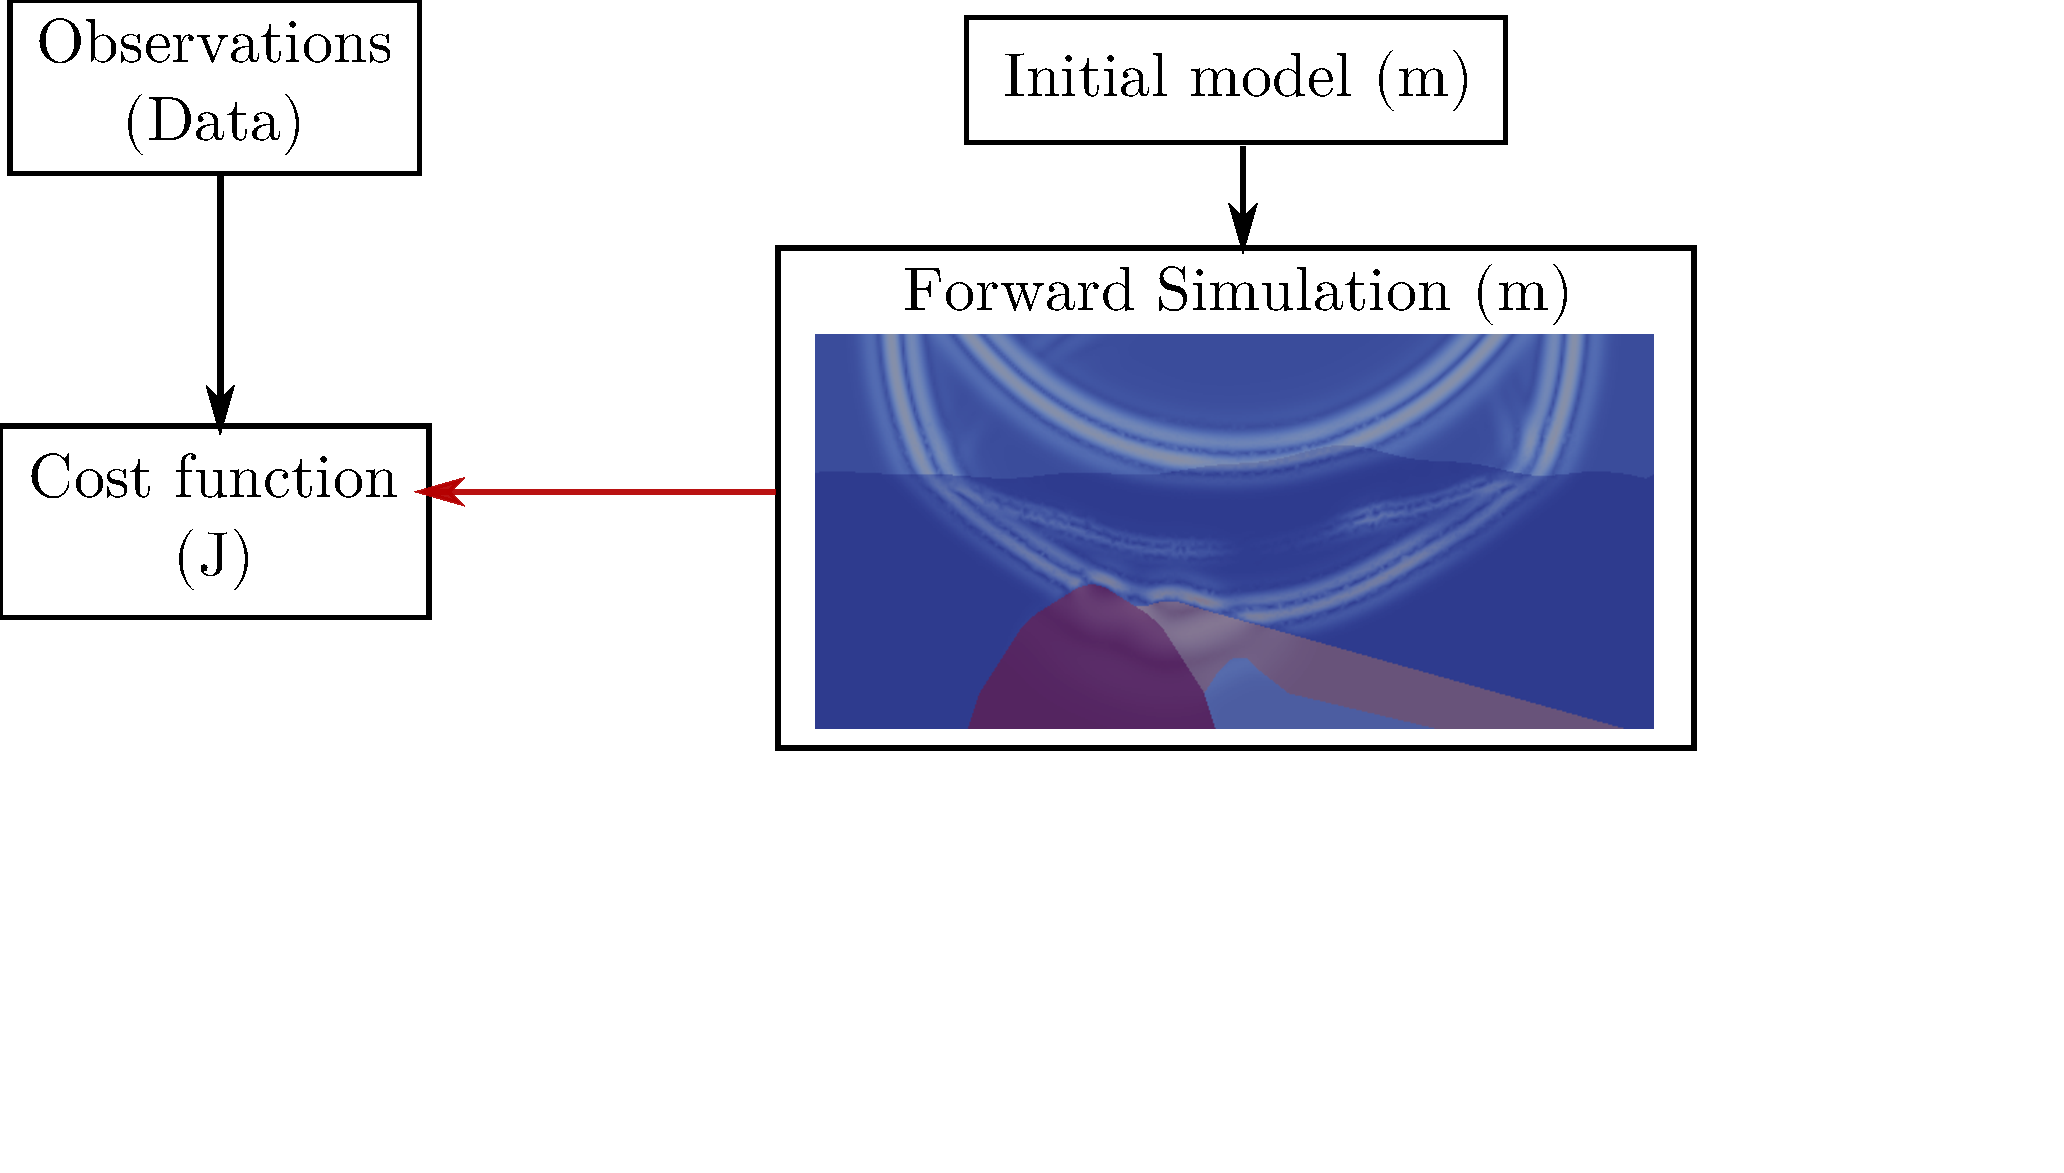
\includegraphics[scale=0.31]{fwi_test1.pdf}
\end{figure}
\end{frame}

\begin{frame}[noframenumbering]{FWI Workflow}
\begin{figure}
  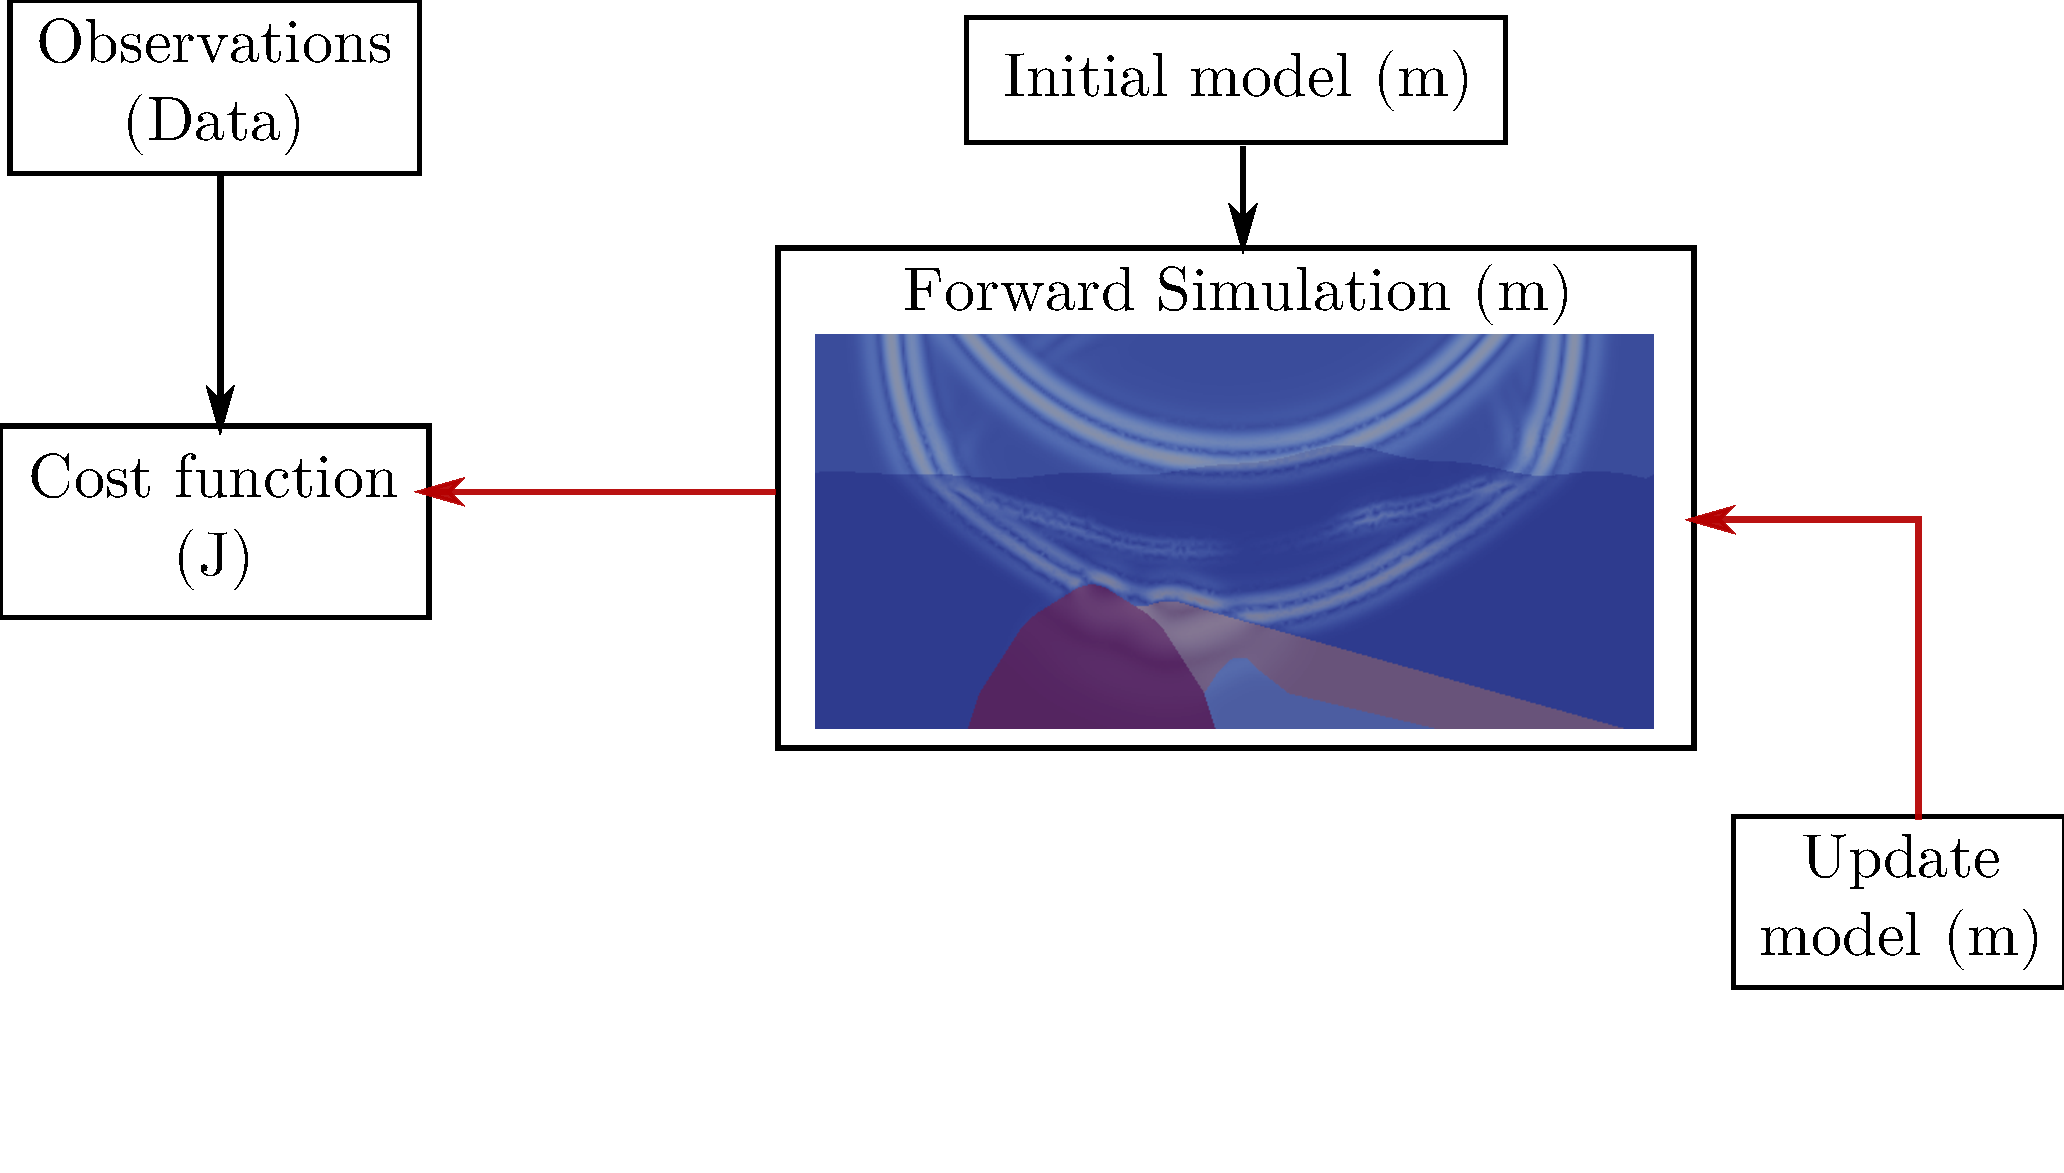
\includegraphics[scale=0.31]{fwi_test2.pdf}
\end{figure}
\end{frame}


\begin{frame}[noframenumbering]{FWI Workflow}
\begin{figure}
  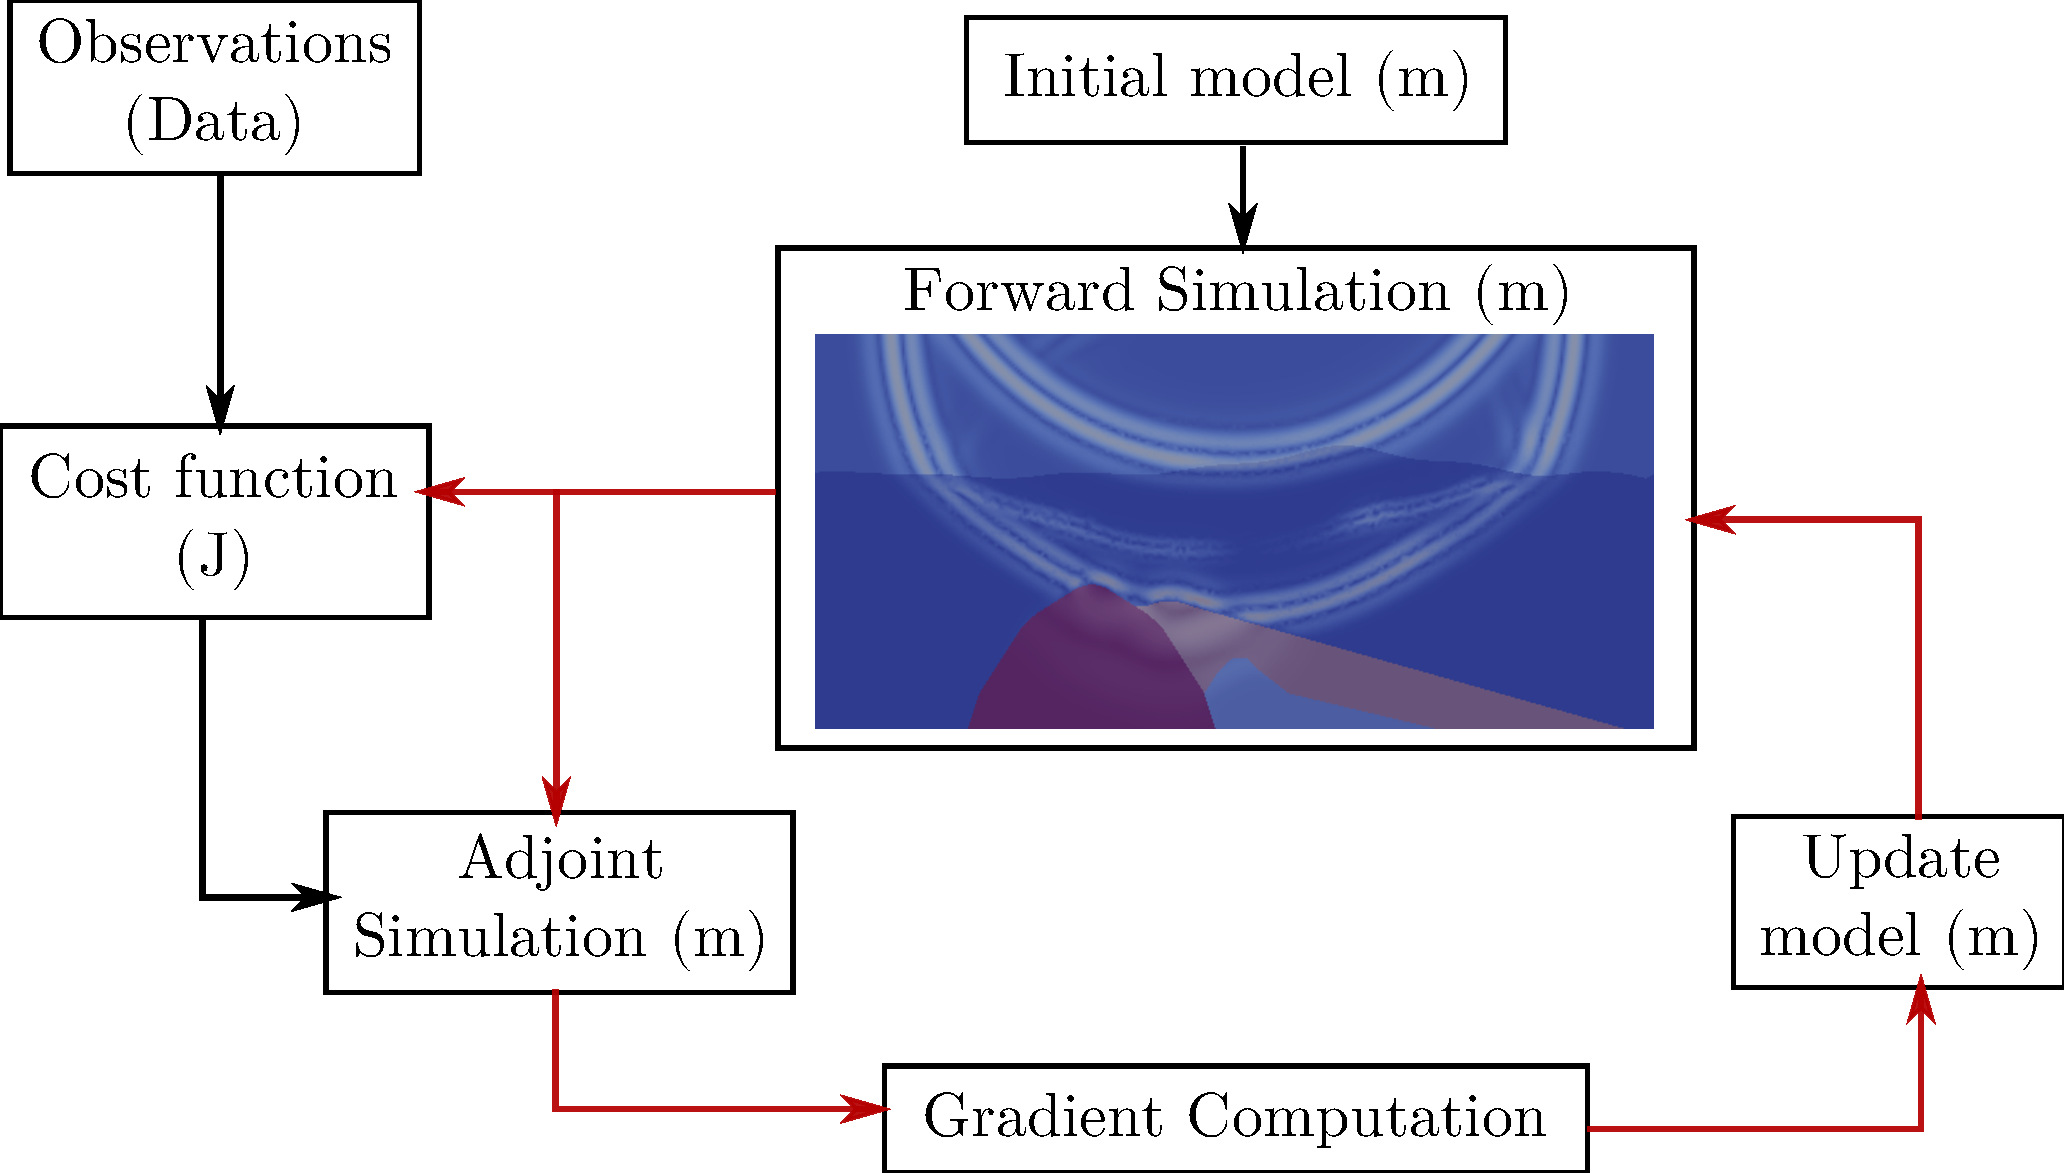
\includegraphics[scale=0.31]{fwi_test.pdf}
\end{figure}
\end{frame}

\begin{frame}[noframenumbering]{FWI Workflow}
\begin{figure}
  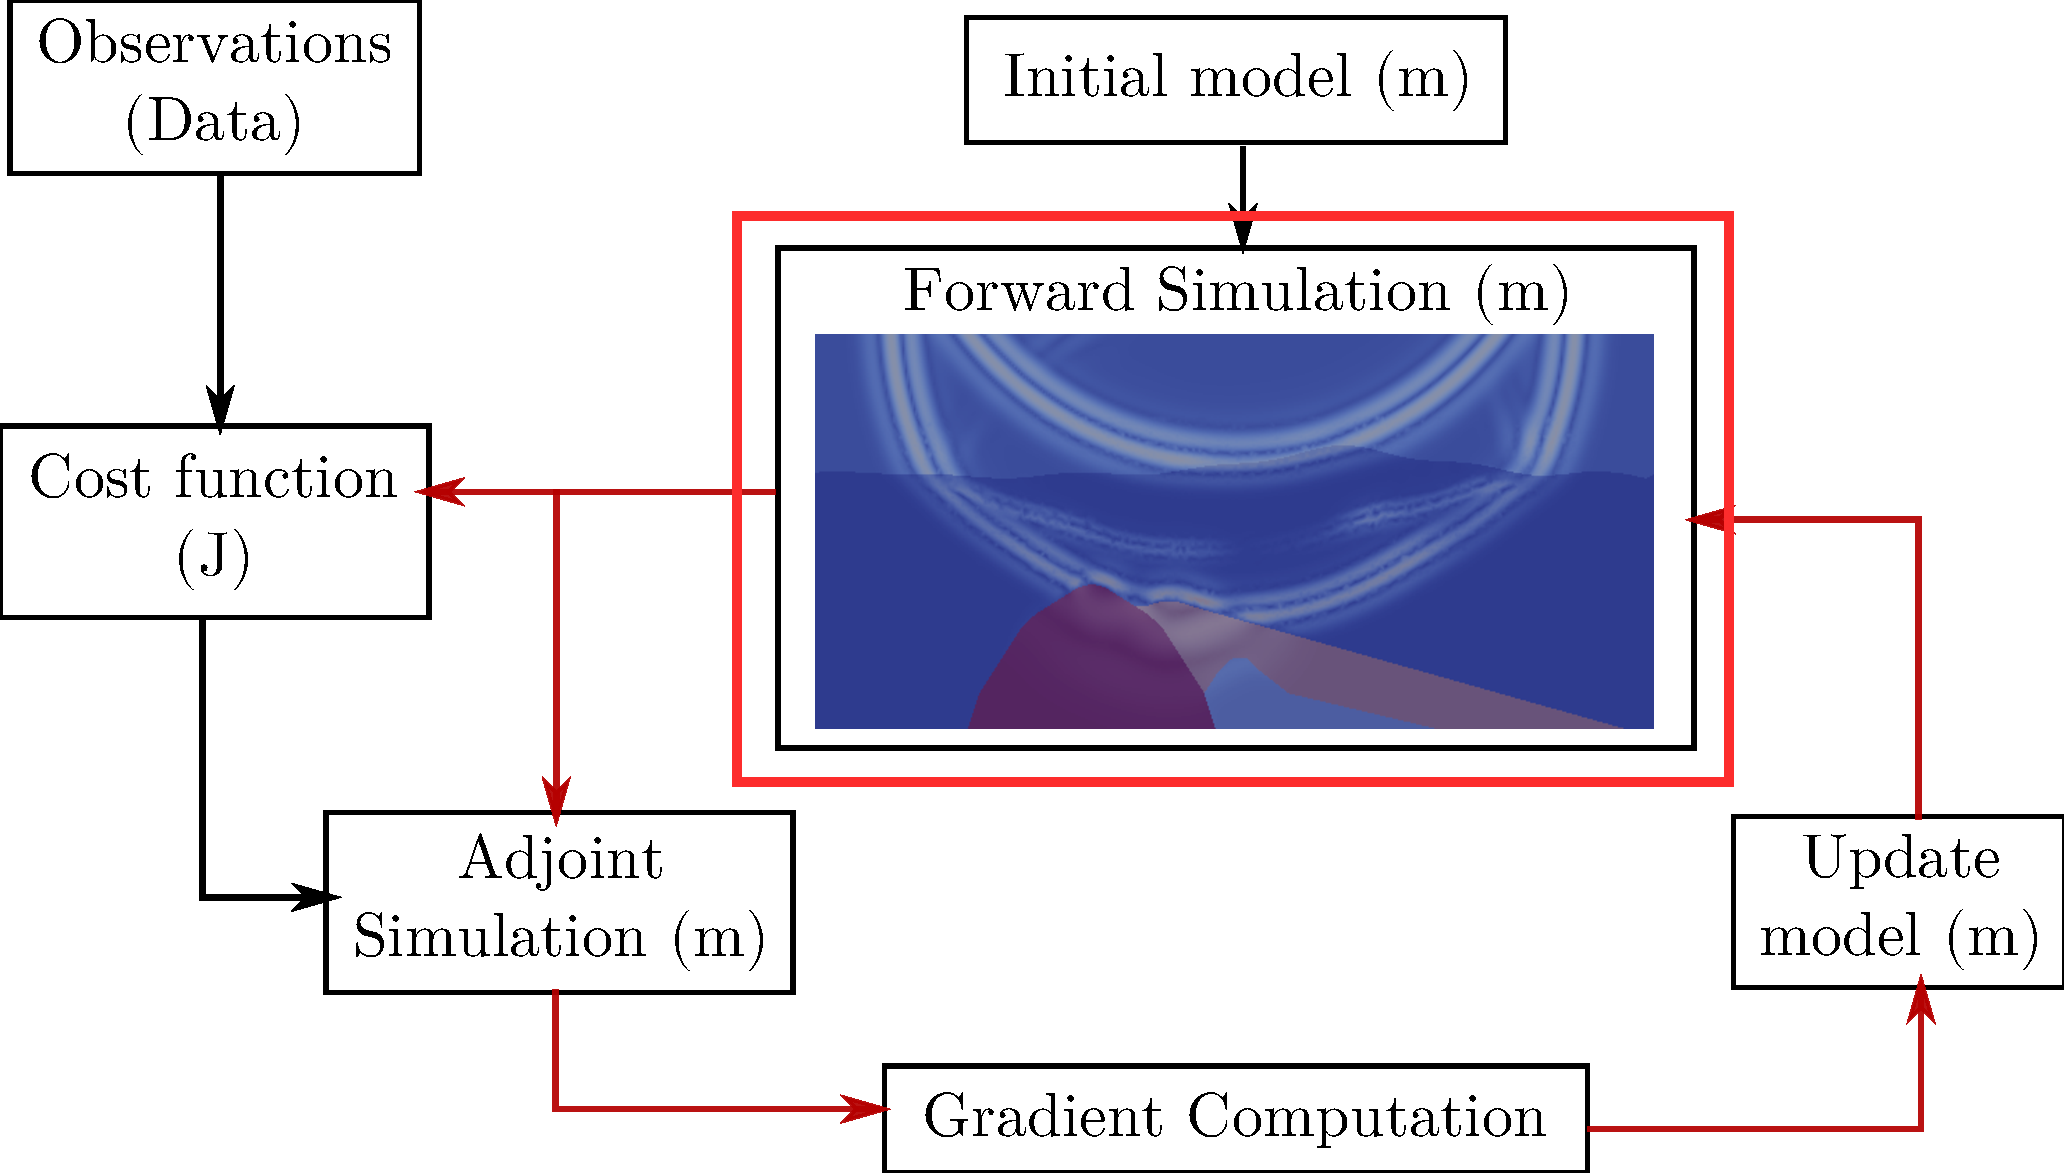
\includegraphics[scale=0.31]{fwi_test3.pdf}
\end{figure}
\end{frame}



% ============================================
% ====== Frame : Forward Continuous Model ====
% ============================================

\subsection{Forward Discretization}
\begin{frame}{Continuous Forward Model}

  First order acoustic wave equation
  \begin{multicols}{2}
  \begin{empheq}[left=\empheqlbrace]{align}
    & \frac{1}{\density \velocity^2}\frac{\partial \contP}{\partial t}+\nabla \cdot \contV=f_p \text{~~ on $\boldsymbol{\Omega}$}\\
    & \density\frac{\partial \contV}{\partial t}+\nabla\contP=0  \text{~~ on $\boldsymbol{\Omega}$}\\
    & \contP=0 \text{~~ on $\textcolor{red}{\boldsymbol{\Gamma_1}}$} \\
    & \frac{\partial \contP}{\partial t}+\velocity \nabla \contP \cdot \normal=0 \text{~~ on $\textcolor{blue}{\boldsymbol{\Gamma_2}}$}
  \end{empheq}

  \columnbreak

  \begin{center}
    \renewcommand\tikzscale{1.0}
    \begin{figure}[H]
    \begin{tikzpicture}[scale=\tikzscale]
\draw[color=blue,line width=2,double] (0,0) -- (5,0);
\draw[color=blue,line width=2,double] (0.07,-0.07) -- (0.07,3);
\draw[color=blue,line width=2,double] (4.93,-0.07) -- (4.93,3);
\draw[color=red,line width=2.1](-0.,3) -- (5,3);


\node[anchor=south, color=red]
at (2.5,3) {$\Gamma_1$};

\node[anchor=south, color=blue]
at (2.5,0) {$\Gamma_2$};

\node[color=black]
at (2.5,1.5) {$\Omega$};
\end{tikzpicture}

    \small{Domain with Absorbing Boundary Conditions}
    \end{figure}
  \end{center}

  \end{multicols}
\end{frame}





% ============================================
% ====== Frame : Forward Discrete Model ======
% ============================================

\begin{frame}{Discrete Forward Model}

  \begin{multicols}{2}

    Space Discretization : Discontinuous Galerkin Elements
    \begin{itemize}
      \item Nodal \small{(Lagrangian / Jacobian)}
      \item \normalsize{Modal} \small{(Bernstein-Bézier)}
    \end{itemize}
    \vspace{1cm}
    \uncover<3->{
    Time schemes :
    \begin{itemize}
      \item Runge Kutta 2/4
      \item Adams Bashforth 3
    \end{itemize}}

    \columnbreak

    \uncover<2->{
    Semi-discretized model :
    \begin{equation}
      \frac{\partial}{\partial t}\discreteU(t) = A \discreteU(t) + \discreteF(t)
    \end{equation}

    with :

    \begin{equation}
      \discreteU(t)=\vectll{(}{\discreteP(t)}{\discreteV(t)}{)}
    \end{equation}}

    \uncover<3->{
    \begin{figure}
      \noindent
       \begin{tikzpicture}[scale=0.8]
      \draw[color=black,line width=2.1](0.0,0.0) -- (5,0.0);
      %\draw[color=blue, line width=10] (0,-0.02) node {$\bullet$} ;
      %\draw[color=blue, line width=10] (5,-0.02) node {$\bullet$} ;
     % \draw node[color=blue,fill,circle,minimum size=0.01](1,1) {};
      \node[anchor=south east, color=black]
      at (0,0) {$0$};
      \node[anchor=south west, color=black]
      at (5,0) {$T$};
      
      \pgfmathsetmacro{\x}{0.0}
      \draw[color=black,line width=2.1](\x,0.1) -- (\x,-0.1);

      \pgfmathsetmacro{\x}{5.0}
      \draw[color=black,line width=2.1](\x,0.1) -- (\x,-0.1);

      \pgfmathsetmacro{\x}{0.5}
      \draw[color=black,line width=1.5](\x,0.1) -- (\x,-0.1);
      \draw[arrowStyle,color=blue]
      (\x-0.5,0) to[out=90,in=90,looseness=4.0]
      node[sloped,anchor=south]
      {}
      (\x,0.0);
      \draw[color=black,line width=1.5](\x,0.1) -- (\x,-0.1);


      
      \pgfmathsetmacro{\x}{1.0}
            \draw[arrowStyle,color=blue]
      (\x-0.5,0) to[out=90,in=90,looseness=4.0]
      node[sloped,anchor=south]
      {}
      (\x,0.0);
      \draw[color=black,line width=1.5](\x,0.1) -- (\x,-0.1);
      \pgfmathsetmacro{\x}{1.5}
            \draw[arrowStyle,color=blue]
      (\x-0.5,0) to[out=90,in=180,looseness=1.0]
      node[sloped,anchor=south]
      {}
      (\x,0.55);

      
      \draw[color=black,line width=1.5](\x,0.1) -- (\x,-0.1);
      \pgfmathsetmacro{\x}{2.0}
      \draw[color=black,line width=1.5](\x,0.1) -- (\x,-0.1);
      \pgfmathsetmacro{\x}{2.5}
      \draw[color=black,line width=1.5](\x,0.1) -- (\x,-0.1);
      \pgfmathsetmacro{\x}{3.0}
      \draw[color=black,line width=1.5](\x,0.1) -- (\x,-0.1);
      \pgfmathsetmacro{\x}{3.5}
      \draw[color=black,line width=1.5](\x,0.1) -- (\x,-0.1);
      \pgfmathsetmacro{\x}{4.0}
      \draw[color=black,line width=1.5](\x,0.1) -- (\x,-0.1);
      \pgfmathsetmacro{\x}{4.5}
      \draw[color=black,line width=1.5](\x,0.1) -- (\x,-0.1);
    \end{tikzpicture}

      Forward time steps
    \end{figure}}

  \end{multicols}

\end{frame}






% ============================================
% ====== Frame : Asset of DGs  ===============
% ============================================

\begin{frame}{Discrete Forward Model}{Discontinuous Galerkin Method}
  Asset of Discontinuous Galerkin Methods : \\

  \begin{itemize}
  \item Unstructured grid (enable to match the topography and media irregularities)
  \item Robust to physical discontinuities
  \item hp-adaptivity
  \item Massively parallel performance properties
  \end{itemize}

  \begin{figure}[H]
    \centering
    \subfigure[h-adaptivity]{
      \begin{tikzpicture}[scale=0.7]%[line cap=round,line join=round,>=triangle 45,x=1.0cm,y=1.0cm]
      %% \draw[->,color=black] (-1.05,0) -- (9.66,0);
      %% \foreach \x in {-1,-0.5,0.5,1,1.5,2,2.5,3,3.5,4,4.5,5,5.5,6,6.5,7,7.5,8,8.5,9,9.5}
      %% \draw[shift={(\x,0)},color=black] (0pt,2pt) -- (0pt,-2pt) node[below] {\footnotesize $\x$};
      %% \draw[->,color=black] (0,-0.43) -- (0,5.53);
      %% \foreach \y in {,0.5,1,1.5,2,2.5,3,3.5,4,4.5,5,5.5}
      %% \draw[shift={(0,\y)},color=black] (2pt,0pt) -- (-2pt,0pt) node[left] {\footnotesize $\y$};
      %% \draw[color=black] (0pt,-10pt) node[right] {\footnotesize $0$};
      %% \clip(-1.05,-0.43) rectangle (9.66,5.53);
      \fill[line width=2.4pt,fill=black,fill opacity=0.1] (1,1) -- (4,2) -- (4,1) -- cycle;
      \fill[line width=2.4pt,fill=black,fill opacity=0.1] (1,1) -- (1,4) -- (2,4) -- cycle;
      \fill[line width=2.4pt,fill=black,fill opacity=0.1] (2,4) -- (4,2) -- (1,1) -- cycle;
      \fill[line width=2.4pt,fill=black,fill opacity=0.1] (2,4) -- (4,4) -- (4,2) -- cycle;
      \draw [line width=2.4pt] (1,1)-- (4,2);
      \draw [line width=2.4pt] (4,2)-- (4,1);
      \draw [line width=2.4pt] (4,1)-- (1,1);
      \draw [line width=2.4pt] (1,1)-- (1,4);
      \draw [line width=2.4pt] (1,4)-- (2,4);
      \draw [line width=2.4pt] (2,4)-- (1,1);
      \draw [line width=2.4pt] (2,4)-- (4,2);
      \draw [line width=2.4pt] (4,2)-- (1,1);
      \draw [line width=2.4pt] (1,1)-- (2,4);
      \draw [line width=2.4pt] (2,4)-- (4,4);
      \draw [line width=2.4pt] (4,4)-- (4,2);
      \draw [line width=2.4pt] (4,2)-- (2,4);
      \draw [line width=2.4pt] (2,4)-- (3.5,3.5);
      \draw [line width=2.4pt] (3,3)-- (4,4);
      \draw [line width=2.4pt] (4,4)-- (2,4);
      \draw [line width=2.4pt] (2,4)-- (3.5,3.5);
      \draw [line width=2.4pt] (3.5,3.5)-- (4,2);
      \draw [line width=2.4pt] (4,2)-- (2,4);
      \draw [line width=2.4pt] (4,2)-- (4,4);
      \draw [line width=2.4pt] (4,4)-- (3.5,3.5);
      \draw [line width=2.4pt] (3.5,3.5)-- (4,2);
  \end{tikzpicture}

}
    \hspace{1cm}
  \subfigure[p-adaptivity with \textcolor{black}{P1}, \textcolor{blue}{P2}, \textcolor{red}{P3} elements]{
      \definecolor{ccqqqq}{rgb}{0.8,0,0}
    \definecolor{qqqqff}{rgb}{0,0,1}
    \definecolor{cccccc}{rgb}{0.8,0.8,0.8}
    \begin{tikzpicture}[scale=0.7]
      %\draw[->,color=black] (0,0.62) -- (0,4.91);
      %\foreach \y in {0.6,0.8,1,1.2,1.4,1.6,1.8,2,2.2,2.4,2.6,2.8,3,3.2,3.4,3.6,3.8,4,4.2,4.4,4.6,4.8}
      %\draw[shift={(0,\y)},color=black] (2pt,0pt) -- (-2pt,0pt) node[left] {\footnotesize $\y$};
      %\clip(-0.64,0.62) rectangle (7.09,4.91);
      \fill[line width=1.6pt,color=cccccc,fill=cccccc,fill opacity=0.15] (1,1) -- (1,4) -- (4,4) -- (4,1) -- cycle;
      \fill[fill=black,fill opacity=0.1] (1,1) -- (2.5,2.5) -- (4,1) -- cycle;
      \fill[fill=black,fill opacity=0.1] (1,1) -- (2.5,2.5) -- (1,4) -- cycle;
      \fill[fill=black,fill opacity=0.1] (1,4) -- (4,4) -- (2.5,2.5) -- cycle;
      \fill[fill=black,fill opacity=0.1] (4,1) -- (2.5,2.5) -- (4,4) -- cycle;
      \draw [line width=2.8pt] (1,1)-- (1,4);
      \draw [line width=2.8pt] (1,4)-- (4,4);
      \draw [line width=2.8pt] (4,4)-- (4,1);
      \draw [line width=2.8pt] (4,1)-- (1,1);
      \draw [line width=2.8pt] (1,1)-- (2.5,2.5);
      \draw [line width=2.8pt] (2.5,2.5)-- (4,1);
      \draw [line width=2.8pt] (4,1)-- (1,1);
      \draw [line width=2.8pt] (1,1)-- (2.5,2.5);
      \draw [line width=2.8pt] (2.5,2.5)-- (1,4);
      \draw [line width=2.8pt] (1,4)-- (1,1);
      \draw [line width=2.8pt] (1,4)-- (4,4);
      \draw [line width=2.8pt] (4,4)-- (2.5,2.5);
      \draw [line width=2.8pt] (2.5,2.5)-- (1,4);
      \draw [line width=2.8pt] (4,1)-- (2.5,2.5);
      \draw [line width=2.8pt] (2.5,2.5)-- (4,4);
      \draw [line width=2.8pt] (4,4)-- (4,1);
      \begin{scriptsize}
        \fill [color=black] (1.07,3.76) circle (2.321pt);
        \fill [color=black] (1.08,1.24) circle (2.321pt);
        \fill [color=black] (2.3,2.5) circle (2.321pt);
        \fill [color=qqqqff] (2.51,2.3) circle (2.321pt);
        \fill [color=qqqqff] (2.72,2.5) circle (2.321pt);
        \fill [color=ccqqqq] (2.5,2.71) circle (2.321pt);
        \fill [color=qqqqff] (3.77,1.09) circle (2.321pt);
        \fill [color=qqqqff] (3.91,1.22) circle (2.321pt);
        \fill [color=ccqqqq] (3.73,3.87) circle (2.321pt);
        \fill [color=qqqqff] (3.89,3.75) circle (2.321pt);
        \fill [color=qqqqff] (1.24,1.11) circle (2.321pt);
        \fill [color=qqqqff] (1.87,1.7) circle (2.321pt);
        \fill [color=qqqqff] (3.14,1.69) circle (2.321pt);
        \fill [color=qqqqff] (2.51,1.1) circle (2.321pt);
        \fill [color=qqqqff] (3.31,1.86) circle (2.321pt);
        \fill [color=qqqqff] (3.9,2.48) circle (2.321pt);
        \fill [color=qqqqff] (3.31,3.13) circle (2.321pt);
        \fill [color=ccqqqq] (1.23,3.9) circle (2.321pt);
        \fill [color=ccqqqq] (2.08,3.87) circle (2.321pt);
        \fill [color=ccqqqq] (2.97,3.86) circle (2.321pt);
        \fill [color=ccqqqq] (1.63,3.56) circle (2.321pt);
        \fill [color=ccqqqq] (2.15,3.06) circle (2.321pt);
        \fill [color=ccqqqq] (3.36,3.54) circle (2.321pt);
        \fill [color=ccqqqq] (2.83,3.05) circle (2.321pt);
        \fill [color=ccqqqq] (2.49,3.55) circle (2.321pt);
      \end{scriptsize}
  \end{tikzpicture}

  }
\end{figure}
\end{frame}
  %% intro FWI
%% \section{Adjoint Studies}
\renewcommand\tikzscale{1.3}


% ============================================
% ====== Frame : Adjoint State Method  =======
% ============================================

\begin{frame}{Adjoint State Method}

Lagrangian fonctional :
  \begin{equation}
    \Lag(\qcqU,\qcqLbd,\model) = \frac{1}{2}||\textcolor{blue}{d_{obs}}-\textcolor{red}{\mathcal{R}(\qcqU)}||^2dt + <\DP(\qcqU),\qcqLbd>
  \end{equation}

    If $\qcqU=\contU$ Solution of the Direct Problem $\Longleftrightarrow$ ($\DP(\contU) = 0$) :

  \begin{equation}
    \CF(\model) = \Lag(\contU,\qcqLbd,\model)
  \end{equation}

  \uncover<2->{
  Let us choose $\qcqLbd=\contLbd$ such as $\frac{\partial \Lag}{\partial \contU} = 0$

  \begin{equation}
    (\mathcal{R}^*\textcolor{blue}{d_{obs}}-\contU) + \DP^*(\contLbd) = 0
  \end{equation}
  }

  \uncover<3->{
  For $\DP(\contU) = 0$ :

  \begin{equation}
    \partial_{\model_i} \CF(\model) = \partial_{\model_i} \Lag(\contU,\contLbd,\model) = \partial_{\model_i} <\DP(\contU),\contLbd>
  \end{equation}
}

\end{frame}











% ============================================
% ====== Frame : Adjoint Scheme      =========
% ============================================
\begin{frame}{Adjoint Formulation}
\begin{figure}

\definecolor{color1}{RGB}{255,174,41}   %% myOrange
%\definecolor{color2}{RGB}{216,93,99}  %% myGreen
\definecolor{color3}{RGB}{100,149,237} %% myBlue
\definecolor{color2}{RGB}{223,83,74} %% myRed

\definecolor{colorOne}{RGB}{255,174,41}   %% myOrange
%\definecolor{color2}{RGB}{216,93,99}  %% myGreen
\definecolor{colorThree}{RGB}{100,149,237} %% myBlue
\definecolor{colorTwo}{RGB}{223,83,74} %% myRed


\begin{tikzpicture}[scale=\tikzscale] %% [every node/.style={scale=1}]

\node[boxOptions]
at (0,3.5){ {\textbf{\Large\fontfamily{pzc}\selectfont Continuous \\ Direct Problem}}};

\uncover<2->{
\node[boxOptions]
at (6,3.5){ {\textbf{\Large\fontfamily{pzc}\selectfont Continuous \\ Adjoint Problem}}};

\coordinate (a) at (1.4,3.5);
\coordinate (b) at (4.7,3.5);
\draw[->, >=latex, red!50!white, line width=10pt]   (a) to node[pos=0.4,above]{\small{\textbf{\textcolor{black}{Adjoint}}}} (b) ;
}

\uncover<3->{
\node[boxOptions]
at (6,0.7){\textbf{Discretization of the Continuous Adjoint Problem}};

\draw[arrowStyleinv]
(6,2.1) to[out=90,in=90]
node[sloped,anchor=south]
{}
(6,2.6);

\coordinate (b) at (6,1.2);
\coordinate (a) at (6,3.0);
\draw[->, >=latex, red!50!white, line width=10pt]   (a) to node[fill=colorThree!0,pos=0.3]{\small{\textbf{\textcolor{black}{Discretization}}}} (b) ;
}


\uncover<4->{
\node[boxOptions]
at (0,-0.5){\textbf{Discrete \\Direct Problem}};

%% \draw[arrowStyleinv]
%% (0,0.7) to[out=90,in=90]
%% node[sloped,anchor=south]
%% {\footnotesize{Discretization ~~~~~~~~~~~~~}}
%% (0,2.5);

\coordinate (b) at (0,-0.1);
\coordinate (a) at (0,3.0);
\draw[->, >=latex, blue!50!white, line width=10pt]   (a) to node[fill=colorThree!0]{\small{\textbf{\textcolor{black}{Discretization}}}} (b) ;


\node[boxOptions]
at (6,-0.5){\textbf{Adjoint of the Discrete Problem}};


%% \draw[arrowStyle]
%% (2,0) to[out=0,in=180]
%% node[sloped,anchor=south]
%% {(*)}
%% (4,0);

\coordinate (a) at (1.4,-0.5);
\coordinate (b) at (4.7,-0.5);
\draw[->, >=latex, blue!50!white, line width=10pt]   (a) to node[pos=0.4,below]{\small{\textbf{\textcolor{black}{Adjoint}}}} (b) ;
}

\uncover<5->{
\draw[color=red,line width=2] (4.5,1.4)
rectangle (7.5,-1.0);
}
\end{tikzpicture}
\end{figure}
\end{frame}








% ============================================
% ====== Frame : Adjoint then discretize 1 ===
% ============================================

\begin{frame}{AtD : Adjoint then Discretized Strategy}

  \begin{equation}
    \CF(\contP)=\frac{1}{2}||\textcolor{blue}{d_{obs}} - R\contP||^2
    \end{equation}

  \noindent
  \begin{multicols}{2}
    \noindent
      \begin{empheq}[left=\empheqlbrace]{align}
    & \frac{1}{\density \velocity^2}\frac{\partial \contP}{\partial t}+\nabla \cdot \contV=f_p \text{~~ on $\boldsymbol{\Omega}$}\\
    & \density\frac{\partial \contV}{\partial t}+\nabla\contP=0  \text{~~ on $\boldsymbol{\Omega}$}\\
    & \contP=0 \text{~~ on $\textcolor{red}{\boldsymbol{\Gamma_1}}$} \\
    & \frac{\partial \contP}{\partial t}+\velocity \nabla \contP \cdot \normal=0 \text{~~ on $\textcolor{blue}{\boldsymbol{\Gamma_2}}$}\\
    & \contP(0) = 0 \text{, ~~~} \contV(0) = 0
      \end{empheq}
      \vspace{30cm}
    \columnbreak
    \noindent
      \begin{empheq}[left=\empheqlbrace]{align}
    & \frac{1}{\density \velocity^2}\frac{\partial \Lbdun}{\partial t}+\nabla \cdot \Lbdeux=\frac{\partial \CF}{\partial \contP} \text{~~ on $\boldsymbol{\Omega}$}\\
    & \density\frac{\partial \Lbdeux}{\partial t}+\nabla\Lbdun=0  \text{~~ on $\boldsymbol{\Omega}$}\\
    & \Lbdun=0 \text{~~ on $\textcolor{red}{\boldsymbol{\Gamma_1}}$} \\
    & \frac{\partial \Lbdun}{\partial t}-\velocity \nabla \Lbdun \cdot \normal=0 \text{~~ on $\textcolor{blue}{\boldsymbol{\Gamma_2}}$}\\
    & \Lbdun(T) = 0 \text{, ~~~} \Lbdeux(T) = 0
  \end{empheq}

  \end{multicols}
  \vspace{-0.5cm}
  \begin{equation}
    t\in[0,T] \text{~~~~~~~~~~~~~~~~~~~~~~~~~~} t\in[T,0]
    \end{equation}
\end{frame}





% ============================================
% ====== Frame : Adjoint then discretize 2 ===
% ============================================

\subsection{Adjoint then Discretized}
\begin{frame}{AtD : Adjoint then Discretized Strategy}

  \begin{equation}
    \CF(\contP)=\frac{1}{2}||\textcolor{blue}{d_{obs}} - R\contP||^2
  \end{equation}

  \noindent
  \begin{multicols}{2}
    \noindent
    \begin{empheq}[left=\empheqlbrace]{align}
  & \frac{\partial \discreteU}{\partial t}^n=A\discreteU^n+ \discreteF^n \\[0.2cm]
  & \text{With : ~~}  \discreteU^n=\vectll{(}{\discreteP^n}{\discreteV^n}{)}
    \end{empheq}
    \vspace{0.3cm}
    \begin{figure}
      \noindent
       \begin{tikzpicture}[scale=0.8]
      \draw[color=black,line width=2.1](0.0,0.0) -- (5,0.0);
      %\draw[color=blue, line width=10] (0,-0.02) node {$\bullet$} ;
      %\draw[color=blue, line width=10] (5,-0.02) node {$\bullet$} ;
     % \draw node[color=blue,fill,circle,minimum size=0.01](1,1) {};
      \node[anchor=south east, color=black]
      at (0,0) {$0$};
      \node[anchor=south west, color=black]
      at (5,0) {$T$};
      
      \pgfmathsetmacro{\x}{0.0}
      \draw[color=black,line width=2.1](\x,0.1) -- (\x,-0.1);

      \pgfmathsetmacro{\x}{5.0}
      \draw[color=black,line width=2.1](\x,0.1) -- (\x,-0.1);

      \pgfmathsetmacro{\x}{0.5}
      \draw[color=black,line width=1.5](\x,0.1) -- (\x,-0.1);
      \draw[arrowStyle,color=blue]
      (\x-0.5,0) to[out=90,in=90,looseness=4.0]
      node[sloped,anchor=south]
      {}
      (\x,0.0);
      \draw[color=black,line width=1.5](\x,0.1) -- (\x,-0.1);


      
      \pgfmathsetmacro{\x}{1.0}
            \draw[arrowStyle,color=blue]
      (\x-0.5,0) to[out=90,in=90,looseness=4.0]
      node[sloped,anchor=south]
      {}
      (\x,0.0);
      \draw[color=black,line width=1.5](\x,0.1) -- (\x,-0.1);
      \pgfmathsetmacro{\x}{1.5}
            \draw[arrowStyle,color=blue]
      (\x-0.5,0) to[out=90,in=180,looseness=1.0]
      node[sloped,anchor=south]
      {}
      (\x,0.55);

      
      \draw[color=black,line width=1.5](\x,0.1) -- (\x,-0.1);
      \pgfmathsetmacro{\x}{2.0}
      \draw[color=black,line width=1.5](\x,0.1) -- (\x,-0.1);
      \pgfmathsetmacro{\x}{2.5}
      \draw[color=black,line width=1.5](\x,0.1) -- (\x,-0.1);
      \pgfmathsetmacro{\x}{3.0}
      \draw[color=black,line width=1.5](\x,0.1) -- (\x,-0.1);
      \pgfmathsetmacro{\x}{3.5}
      \draw[color=black,line width=1.5](\x,0.1) -- (\x,-0.1);
      \pgfmathsetmacro{\x}{4.0}
      \draw[color=black,line width=1.5](\x,0.1) -- (\x,-0.1);
      \pgfmathsetmacro{\x}{4.5}
      \draw[color=black,line width=1.5](\x,0.1) -- (\x,-0.1);
    \end{tikzpicture}

Time-steps going Forward
    \end{figure}
    \columnbreak
    \noindent
    \begin{empheq}[left=\empheqlbrace]{align}
   \boldsymbol{~~~}   & \frac{\partial \discreteLbd}{\partial t}^n=A\discreteLbd^n+R^*(R\discreteU^n-\textcolor{blue}{d_{obs}})\\
  & \text{With : ~~}  \discreteLbd^n=\vectll{(}{\discreteLbdun^n}{\discreteLbdeux^n}{)}
    \end{empheq}
    \vspace{-0.0cm}
    \noindent
    \begin{figure}
      \noindent
       \begin{tikzpicture}[scale=0.8]
      \draw[color=black,line width=2.1](0.0,0.0) -- (5,0.0);
      %\draw[color=blue, line width=10] (0,-0.02) node {$\bullet$} ;
      %\draw[color=blue, line width=10] (5,-0.02) node {$\bullet$} ;
     % \draw node[color=blue,fill,circle,minimum size=0.01](1,1) {};
      \node[anchor=south east, color=black]
      at (0,0) {$0$};
      \node[anchor=south west, color=black]
      at (5,0) {$T$};
      
      \pgfmathsetmacro{\x}{0.0}
      \draw[color=black,line width=2.1](\x,0.1) -- (\x,-0.1);

      \pgfmathsetmacro{\x}{5.0}
      \draw[color=black,line width=2.1](\x,0.1) -- (\x,-0.1);

      \pgfmathsetmacro{\x}{0.5}
      \draw[color=black,line width=1.5](\x,0.1) -- (\x,-0.1);
      \draw[color=black,line width=1.5](\x,0.1) -- (\x,-0.1);


      
      \pgfmathsetmacro{\x}{1.0}
      \draw[color=black,line width=1.5](\x,0.1) -- (\x,-0.1);
      \pgfmathsetmacro{\x}{1.5}
      \draw[color=black,line width=1.5](\x,0.1) -- (\x,-0.1);
      \pgfmathsetmacro{\x}{2.0}
      \draw[color=black,line width=1.5](\x,0.1) -- (\x,-0.1);
      \pgfmathsetmacro{\x}{2.5}
      \draw[color=black,line width=1.5](\x,0.1) -- (\x,-0.1);
      \pgfmathsetmacro{\x}{3.0}
      \draw[color=black,line width=1.5](\x,0.1) -- (\x,-0.1);
      \pgfmathsetmacro{\x}{3.5}


      \draw[arrowStyle,color=blue]
      (\x+0.5,0) to[out=90,in=0,looseness=1.0]
      node[sloped,anchor=south]
      {}
      (\x,0.55);
      

      
      \draw[color=black,line width=1.5](\x,0.1) -- (\x,-0.1);
      \pgfmathsetmacro{\x}{4.0}


      \draw[arrowStyle,color=blue]
      (\x+0.5,0) to[out=90,in=90,looseness=4.0]
      node[sloped,anchor=south]
      {}
      (\x,0.0);
      
      
      \draw[color=black,line width=1.5](\x,0.1) -- (\x,-0.1);
      \pgfmathsetmacro{\x}{4.5}

      \draw[arrowStyle,color=blue]
      (\x+0.5,0) to[out=90,in=90,looseness=4.0]
      node[sloped,anchor=south]
      {}
      (\x,0.0);
      
      \draw[color=black,line width=1.5](\x,0.1) -- (\x,-0.1);
    \end{tikzpicture}

      Time-steps going Backward
    \end{figure}
  \end{multicols}
\end{frame}







\subsection{Discretize then Adjoint}

% ============================================
% ====== Frame : Discretize then Adjoint 1 ===
% ============================================
\begin{frame}{DtA : Discretize then Adjoint Strategy}{Example With RK4}

  All time scheme can be summed-up such as :
  \begin{equation}
    \textcolor{\myblue}{\boldsymbol{L}}\discreteU=\textcolor{\myblue}{\boldsymbol{E}}\discreteF
  \end{equation}

  \small
      RK4 time-scheme leads to :
    \begin{equation}
      \discreteU^{n+1}=B\discreteU^n+\textcolor{\myblue}{\boldsymbol{C_0}}\discreteF^n+\textcolor{\myblue}{\boldsymbol{C_{\frac{1}{2}}}}\discreteF^{n+\frac{1}{2}}+\textcolor{\myblue}{\boldsymbol{C_1}}\discreteF^{n+1}
    \end{equation}

\begin{equation}
  \textcolor{\myblue}{\boldsymbol{L}}\discreteU=\textcolor{\myblue}{\boldsymbol{E}}\discreteF=\discreteG
\end{equation}
\begin{equation}
  \begin{pmatrix}
    I & & & & \\
    -B&I & & & \\
    & -B&I  & & \\
    & & \ddots & \ddots   & \\
    & &  & -B &I \\
    %% \vdots & \ddots & \vdots \\
    %% 0      & \cdots & 1
  \end{pmatrix}
    \begin{pmatrix}
    \discreteU^0 \\
    \discreteU^1 \\
    \discreteU^2 \\
    \vdots \\
    \discreteU^n \\
  \end{pmatrix}=
  \begin{pmatrix}
    \discreteG^0 \\
    \discreteG^1 \\
    \discreteG^2 \\
    \vdots \\
    \discreteG^n \\
  \end{pmatrix}
  \end{equation}
\end{frame}



% ============================================
% ====== Frame : Discretize then Adjoint 2 ===
% ============================================
\begin{frame}{DtA : Discretize then Adjoint Strategy}

    All time scheme can be summed-up such as :
    \begin{equation}
      \textcolor{\myblue}{\boldsymbol{L}}\discreteU=\textcolor{\myblue}{\boldsymbol{E}}\discreteF \uncover<2->{=\discreteG}
    \end{equation}
    We are looking for a Discrete Adjoint state satisfying :
    \begin{equation}
      \textcolor{\myblue}{\boldsymbol{L^*}}\discreteLbd=-R^*(\textcolor{blue}{d_{obs}}-R\discreteU) \uncover<2->{=\discreteD}
    \end{equation}
    With the adjoint operator $\textcolor{\myblue}{\boldsymbol{L^*}}$ satisfying :
      \begin{equation}
    <\textcolor{\myblue}{\boldsymbol{L}}\discreteU,\discreteLbd>=<\discreteU,\textcolor{\myblue}{\boldsymbol{L^*}}\discreteLbd>
      \end{equation}
      \uncover<2->{
        \begin{equation}
        <\discreteG,\discreteLbd>=<\discreteU,\discreteD> \text{~~~(Adjoint Test)}
      \end{equation}


      \begin{center}
        Adjoint test succeeds $\Longleftrightarrow$  operator $\textcolor{\myblue}{\boldsymbol{L^*}}$  well established
      \end{center}
      }
\end{frame}




% ================================================
% ====== Frame : return on RK4 case ==============
% ================================================

\begin{frame}{DtA : Discretize then Adjoint Strategy}{Example with RK4}
\small
      RK4 time-scheme leads to :
    \begin{equation}
      \discreteU^{n+1}=B\discreteU^n+C_0\discreteF^n+C_{\frac{1}{2}}\discreteF^{n+\frac{1}{2}}+C_1\discreteF^{n+1}
    \end{equation}

\begin{equation}
  L\discreteU=E\discreteF=\discreteG
\end{equation}
\begin{equation}
  \begin{pmatrix}
    I & & & & \\
    -B&I & & & \\
    & -B&I  & & \\
    & & \ddots & \ddots   & \\
    & &  & -B &I \\
    %% \vdots & \ddots & \vdots \\
    %% 0      & \cdots & 1
  \end{pmatrix}
  \begin{pmatrix}
    \discreteU^0 \\
    \discreteU^1 \\
    \discreteU^2 \\
    \vdots \\
    \discreteU^n \\
  \end{pmatrix}=
  \begin{pmatrix}
    \discreteG^0 \\
    \discreteG^1 \\
    \discreteG^2 \\
    \vdots \\
    \discreteG^n \\
  \end{pmatrix}
\end{equation}

So :

\begin{equation}
  L^*=\begin{pmatrix}
  I &-B^* & & & \\
  &I &-B^* & & \\
  & &\ddots  &\ddots & \\
  & &  & I   &-B^* \\
  & &  &  &I \\
  %% \vdots & \ddots & \vdots \\
  %% 0      & \cdots & 1
  \end{pmatrix}
\end{equation}
\end{frame}





% ================================================
% ====== Frame : Adjoint Strategies Comparison ===
% ================================================

\begin{frame}{Adjoint Strategies Comparison}
  \begin{columns}
    \begin{column}[t]{0.5\textwidth}
      \textbf{\textcolor{red}{Adjoint Then Discretize}}
      \vspace{0.5cm}
%      \dotfill % to show column margins
      \begin{itemize}
      \item[\textcolor{\mygreen}{\textbf{+}}] Physical approach
      \item[\textcolor{\mygreen}{\textbf{+}}] Same discrete operators for Forward and Backward
      \item[\textbf{- -}] Inaccurate gradient \cite{Sirkes}
      \end{itemize}
      %      \dotfill
      \vspace{0.5cm}
    \end{column}\vrule \hfill
    \begin{column}[t]{0.5\textwidth}
      \textbf{\textcolor{blue}{Discretize then Adjoint}}
      \vspace{0.5cm}
%            \dotfill
      \begin{itemize}
      \item[\textcolor{\mygreen}{\textbf{+}}] Numerical approach
      \item[\textcolor{\mygreen}{\textbf{+}}] Has an Adjoint Test
      \item[\textbf{-}] Tremendous work to develop the adjoint operators
      \item[\textcolor{black}{\textbf{?}}] Non-consistency of the adjoint state \cite{Set1997Feb}
      \end{itemize}
    \end{column}
  \end{columns}

  \vfill
  \tiny
  \begin{thebibliography}{2}
    \bibitem{Sirkes} Sirkes, Ziv and Tziperman, Eli
      \newblock Finite Difference of Adjoint or Adjoint of Finite Difference ?
      \newblock 1997
  \bibitem{Set1997Feb} Sei Alain and Symes William
    \newblock A Note on Consistency and Adjointness for Numerical Schemes
    \newblock 1997
  \end{thebibliography}

\end{frame}
  %% AtD and DtA
%% %\tablesofcontent

\section{Some Results}
\subsection{1D Preliminary tests}
\begin{frame}{1D Preliminary tests}
    \begin{figure}
       \begin{tikzpicture}[scale=1.5]
      \draw[color=black,line width=2.1](0.0,0.0) -- (6.5,0);
      %\draw[color=blue, line width=10] (0,-0.02) node {$\bullet$} ;
      %\draw[color=blue, line width=10] (5,-0.02) node {$\bullet$} ;
     % \draw node[color=blue,fill,circle,minimum size=0.01](1,1) {};
      \node[anchor=south east, color=black]
      at (0,0) {};
      \node[anchor=south west, color=black]
      at (4.0,0.2) {\Large $\velocity$ ?};

      \pgfmathsetmacro{\x}{0.0}
      \draw[color=black,line width=2.1](\x,0.1) -- (\x,-0.1);

      \pgfmathsetmacro{\x}{6.5}
      \draw[color=black,line width=2.1](\x,0.1) -- (\x,-0.1);

      \pgfmathsetmacro{\x}{0.5}
      \draw[color=black,line width=1.5](\x,0.1) -- (\x,-0.1);
      \draw[color=black,line width=1.5](\x,0.1) -- (\x,-0.1);



      \pgfmathsetmacro{\x}{1.0}
      \draw[color=black,line width=1.5](\x,0.1) -- (\x,-0.1);
      \pgfmathsetmacro{\x}{1.5}

      \draw[color=black,line width=1.5](\x,0.1) -- (\x,-0.1);
      \pgfmathsetmacro{\x}{2.0}
      \draw[color=black,line width=1.5](\x,0.1) -- (\x,-0.1);
      \pgfmathsetmacro{\x}{2.5}
      \draw[color=black,line width=1.5](\x,0.1) -- (\x,-0.1);
      \pgfmathsetmacro{\x}{3.0}
      \draw[color=black,line width=1.5](\x,0.1) -- (\x,-0.1);
      \pgfmathsetmacro{\x}{3.5}
      \draw[color=black,line width=1.5](\x,0.1) -- (\x,-0.1);
      \pgfmathsetmacro{\x}{4.0}
      \draw[color=black,line width=1.5](\x,0.1) -- (\x,-0.1);
      \pgfmathsetmacro{\x}{4.5}
      \draw[color=black,line width=1.5](\x,0.1) -- (\x,-0.1);
            \pgfmathsetmacro{\x}{5.0}
      \draw[color=black,line width=1.5](\x,0.1) -- (\x,-0.1);

            \pgfmathsetmacro{\x}{5.5}
      \draw[color=black,line width=1.5](\x,0.1) -- (\x,-0.1);


            \pgfmathsetmacro{\x}{6.0}
      \draw[color=black,line width=1.5](\x,0.1) -- (\x,-0.1);

      \pgfmathsetmacro{\x}{1.5}
      \pgfmathsetmacro{\dx}{0.2}
      \pgfmathsetmacro{\y}{-0.2}
      \pgfmathsetmacro{\dy}{-0.4}
      \node (A) at (\x,\y) {}; % B = 5
      \node (B) at (\x+\dx,\y+\dy) {}; % AC = 3
      \node (C) at (\x-\dx,\y+\dy) {}; % BC = 4
      \node (receiver) at (\x,\y+\dy-0.1) {Receiver}; % BC = 4
     % \draw (A) -- (B) -- (C) -- (A);
      \begin{scope}[on background layer]
        \fill [blue] (A.center) -- (B.center) -- (C.center) -- cycle;
      \end{scope}

            \pgfmathsetmacro{\x}{0.0}
      \pgfmathsetmacro{\dx}{0.2}
      \pgfmathsetmacro{\y}{-0.2}
      \pgfmathsetmacro{\dy}{-0.4}
      \node (A) at (\x,\y) {}; % B = 5
      \node (B) at (\x+\dx,\y+\dy) {}; % AC = 3
      \node (C) at (\x-\dx,\y+\dy) {}; % BC = 4
      \node (source) at (\x,\y+\dy-0.1) {Source}; % BC = 4
      %\draw [red] (A) -- (B) -- (C) -- (A);
      \begin{scope}[on background layer]
        \fill [red] (A.center) -- (B.center) -- (C.center) -- cycle;
      \end{scope}
\end{tikzpicture}

    \end{figure}

    \begin{multicols}{2}

      \begin{center}
        Initial $\velocity$ Model
      \end{center}
      \vspace{-0.1cm}

      \setlength{\plotwidth} {4.0cm}
      \setlength{\plotheight}{3cm}
      \begin{figure}
        \centering
          \begin{tikzpicture}
      \begin{axis}[%
          width=\plotwidth, height=\plotheight,,
          at={(0,0)},scale only axis,separate axis lines,xminorticks=true,
          xlabel={Depth},
          %ylabel={$\velocity$},
          %%   ymode=log,
          yminorticks=true,
          %xmin=0.,xmax=100.,
          ymin=0.98,ymax=1.22
        ]

        %% load current data
        %% -----------------
        \addplot[color=blue!50!black,mark options={solid},
          forget plot,line width=1pt,
          mark size=2pt]
        table[x=monx,y=mony]
        {images/VP0.dat};
        %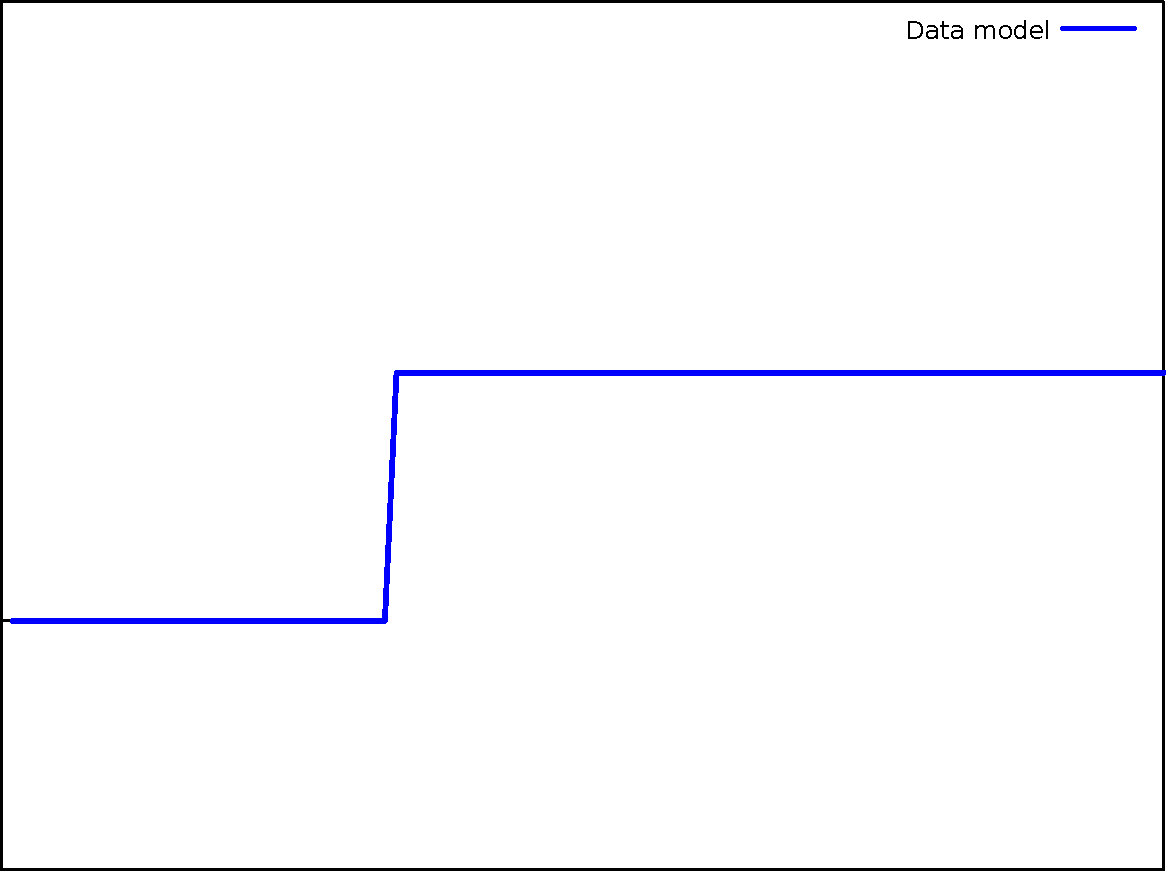
\includegraphics{images/data_bis.pdf}
      \end{axis}
      %% --------------------------------------------------------------------
          \end{tikzpicture}
          \end{figure}

      \columnbreak

      \begin{center}
        Target $\velocity$ Model
      \end{center}
      \vspace{-1.5cm}

      \begin{figure}
        \centering
          \begin{tikzpicture}
      \begin{axis}[%
          width=\plotwidth, height=\plotheight,,
          at={(0,0)},scale only axis,separate axis lines,xminorticks=true,
          xlabel={Depth},
          %ylabel={$\velocity$},
          %%   ymode=log,
          yminorticks=true,
          %%   xmin=0.,xmax=100.
        ]

        %% load current data
        %% -----------------
        \addplot[color=blue!50!black,mark options={solid},
          forget plot,line width=1pt,
          mark size=2pt]
        table[x=monx,y=mony]
        {images/VP100.dat};
      \end{axis}
      %% --------------------------------------------------------------------
          \end{tikzpicture}
          \end{figure}

      \end{multicols}

\end{frame}


%%%%%%%%%%%%%%%%%%%%%%%%%%%%%%%%%%%%%%%%%%%%% 1 %%%%%%%%%%%%%%%%%%%%%%%%%%%%%%%%%%%%%%%%%%%%%%%%
\begin{frame}{1D Preliminary tests :}
  \begin{multicols}{2}
    \normalsize
1D FWI :
\begin{itemize}
\item Lagrange / B-Bézier Operators
\item RK4 / AB3 time-schemes
\end{itemize}
\vspace{0.5cm}
\uncover<2->{
Adjoint test passed with :
\begin{itemize}
\item With a canonical space inner-product ($<u,v>_X=\sum_i u_iv_i$)
\item With a M-space inner product ($<u,v>_X^M=<Mu,v>_X$)
\end{itemize}}
\columnbreak
Gradient expression :
  \begin{equation}
     \nabla_{{\velocity}}\CF=-\int_0^{T} \int_{\Omega} \frac{2}{\density \velocity^3} \frac{\partial \contP}{\partial t}\Lbdun d\Omega dt
  \end{equation}
  \vspace{0.2cm}
  \\
  \tiny
  \uncover<2->{
\code{./run}\\
\code{----- Adjoint test -------}\\
\code{ inner product U/D   553123.57586755091    }\\
\code{ inner product G/Q   553123.57586756046    }\\
}
  %% ------------------------------------\\
  \uncover<3->{
\code{./run}\\
\code{----- Adjoint test -------}\\
\code{ inner product U/D  -75077.332007383695  }\\
\code{ inner product G/Q  -75077.332007386358  }\\
%------------------------------------\\
\code{./run}\\
\code{----- Adjoint test -------}\\
\code{ inner product U/D   125669.89223600870  }\\
\code{ inner product G/Q   125669.89223600952  }\\
}
%------------------------------------\\
\end{multicols}
\end{frame}
%%%%%%%%%%%%%%%%%%%%%%%%%%%%%%%%%%%%%%%%%%%%% 1 %%%%%%%%%%%%%%%%%%%%%%%%%%%%%%%%%%%%%%%%%%%%%%%%


%%%%%%%%%%%%%%%%%%%%%%%%%%%%%%%%%%%%%%%%%%%%% 2 %%%%%%%%%%%%%%%%%%%%%%%%%%%%%%%%%%%%%%%%%%%%%%%%
\begin{frame}{1D Velocity Model Reconstructions}
  \setlength{\plotwidth} {10.3cm}
  \setlength{\plotheight}{6cm}
  \begin{figure}
    \centering
    \begin{tikzpicture}

      \begin{axis}[width=\plotwidth,
                   height=\plotheight,
                   xlabel={Depth},
                   ylabel={$\velocity$},
                   legend pos=south east]
        \addplot[color=red!90!black,mark options={solid},
          line width=1pt,
          mark size=2pt]
        table[x=monx,y=mony]
        {images/VP_ATD.dat};
        \addlegendentry{Adjoint Then Discretize\footnote{With Bernstein-Bézier elements}}
        \addplot[color=blue!90!black,mark options={solid},
          line width=1pt,
          mark size=2pt]
        table[x=monx,y=mony]
        {images/VP_DTA.dat};
        \addlegendentry{Discretize Then Adjoint\footnote{With canonical scalar product}}
      \end{axis}
    \end{tikzpicture}
  \end{figure}
  \begin{center}
    $\velocity$ Model at the 100th FWI iteration
  \end{center}


\end{frame}


%%%%%%%%%%%%%%%%%%%%%%%%%%%%%%%%%%%%%%%%%%%%% 2 %%%%%%%%%%%%%%%%%%%%%%%%%%%%%%%%%%%%%%%%%%%%%%%%
\begin{frame}{1D Velocity Model Reconstructions}

  \begin{minipage}[top]{0.5\linewidth}
    With RK4 :
  \end{minipage}
  \begin{minipage}[top]{0.4\linewidth}
    ~~~~~~~~~~~~~~~ With AB3 :
  \end{minipage}
  \begin{minipage}[top]{0.5\linewidth}
    \setlength{\plotwidth} {6.0cm}
    \setlength{\plotheight}{5cm}
      \begin{figure}
        \begin{tikzpicture}
          \begin{axis}[width=\plotwidth,
              height=\plotheight,
              ymode = log,
              ylabel near ticks, yticklabel pos=right,
              xlabel={FWI Iterations},
              legend pos=north east]
            \addplot[color=red!90!black,mark options={solid},
              line width=1pt,
              mark size=2pt]
            table[x=monx,y=mony]
            {images/run_atd_rk4_bb.txt};
            \addlegendentry{AtD}
            \addplot[color=blue!90!black,mark options={solid},
              line width=1pt,
              mark size=2pt]
            table[x=monx,y=mony]
            {images/run_dta_rk4_bb.txt};
            \addlegendentry{DtA}
          \end{axis}
        \end{tikzpicture}
      \end{figure}
    \end{minipage}\hfill
    \begin{minipage}[top]{0.5\linewidth}
      \begin{figure}
        \begin{tikzpicture}
          \setlength{\plotwidth} {6.0cm}
          \setlength{\plotheight}{5cm}
          \begin{axis}[width=\plotwidth,
              height=\plotheight,
              xlabel={FWI Iterations},
              ymode = log,
              ylabel={log(Cost Function)},
%              ylabel style={rotate=-90},
              legend pos=north east]
            \addplot[color=red!90!black,mark options={solid},
              line width=1pt,
              mark size=2pt]
            table[x=monx,y=mony]
            {images/run_atd_ab3_bb.txt};
            \addlegendentry{AtD}
            \addplot[color=blue!90!black,mark options={solid},
              line width=1pt,
              mark size=2pt]
            table[x=monx,y=mony]
            {images/run_dta_ab3_bb.txt};
            \addlegendentry{DtA}
          \end{axis}
        \end{tikzpicture}
      \end{figure}
    \end{minipage}

    \uncover<2->{
    \begin{itemize}
      \item For RK4 scheme : Similar convergency
      \item For AB3 scheme : \textcolor{red}{AtD} is slighly better than \textcolor{blue}{DtA}
      \item The slope strongly depends on the optimizer -> Impossibilty to conclude
    \end{itemize}
    }

\end{frame}

%%%%%%%%%%%%%%%%%%%%%%%%%%%%%%%%%%%%%%%%%%%%%%%%%%%%%%%%%%%%%%%%%%%%%%%%
\subsection{2D Time Domain FWI Results}
\begin{frame}{2D Time Domain Reconstruction}

2D FWI :
\begin{itemize}
\item Developped in Total environnement (DIP\footnote{\url{http://dip.inria.fr/}})
\item Nodal Space Operators (Lagrangian/Jacobian)
\item Modal Space Operators (Bernstein-Bézier)
\item Runge Kutta 2/4 and Adams Bashforth time-schemes
\end{itemize}
\vspace{0.5cm}
Discretize Then Adjoint strategy not implemented :
\begin{itemize}
\item Tremendous task in a complex industrial code
\end{itemize}
%% \columnbreak
%% \uncover<2->{
%% Gradient expression :
%%   \begin{equation}
%%      \nabla_{{\velocity}}J=-\int_0^{T} \int_{\Omega} \frac{2}{\density \velocity^3} \frac{\partial \contP}{\partial t}\Lbdun d\Omega dt.
%%   \end{equation}
\end{frame}


\begin{frame}[noframenumbering]{2D Time Domain Reconstruction}

2D FWI :
\begin{itemize}
\item Developped in Total environnement (DIP\footnote{\url{http://dip.inria.fr/}})
\item Nodal Operators (Lagrangian/Jacobian)
\item Modal Operators (Bernstein-Bézier)
\item Runge Kutta 2/4 and Adams Bashforth time-schemes
\end{itemize}
\vspace{0.5cm}
 Gradient expression :
  \begin{equation}
     \nabla_{\boldsymbol{\textcolor{\mygreen}{\frac{1}{\kappa}}}}\CF=\int_0^{T} \int_{\Omega} \frac{\partial \contP}{\partial t}\Lbdun d\Omega dt \text{~~~~ with : } \boldsymbol{\textcolor{\mygreen}{\kappa}}=\density \velocity^2
  \end{equation}
   $\velocity$, $\density$ and  $\boldsymbol{\textcolor{\mygreen}{\kappa}}$  Constant per elements
\end{frame}

\newlength{\modelwidth}
\setlength{\modelwidth}{10.8cm}
\newcommand{\modeltitle}{Initial $\velocity$ Model}

\begin{frame}{2D Time Domain FWI Reconstructions}{Time-schemes comparison}
  \vspace{-0.5cm}
  \renewcommand{\modelfile}{fig/marmousi_noise_ini}
  \begin{figure}
       \begin{tikzpicture}
\pgfmathsetmacro{\xmin} {0.}
\pgfmathsetmacro{\xmax} {12.}
\pgfmathsetmacro{\zmin} {0.}
\pgfmathsetmacro{\zmax} {2.5}

\begin{axis}[%
title={\small{\modeltitle}},
width=1.0\modelwidth,
height=0.4\modelwidth,
axis on top, separate axis lines,
xmin=\xmin, xmax=\xmax, %xlabel={x (km)},
ymin=\zmin, ymax=\zmax, ylabel={depth (km)},
yticklabels={},xticklabels={},
y dir=reverse,
colormap/paraview, colorbar,
point meta min=1.5e-3, point meta max=5.5e-3,
colorbar/width=2.5mm,
]
\addplot [forget plot] graphics [xmin=\xmin,xmax=\xmax,ymin=\zmin,ymax=\zmax] {{\modelfile}.png};
\end{axis}
\end{tikzpicture}%
 \hfill
  \end{figure}
  \vspace{-1cm}
  \renewcommand{\modeltitle}{Target $\velocity$ Model}
  \renewcommand{\modelfile}{fig/marmousi_target}
  \begin{figure}
       \begin{tikzpicture}
\pgfmathsetmacro{\xmin} {0.}
\pgfmathsetmacro{\xmax} {12.}
\pgfmathsetmacro{\zmin} {0.}
\pgfmathsetmacro{\zmax} {2.5}

\begin{axis}[%
title={\small{\modeltitle}},
width=1.0\modelwidth,
height=0.4\modelwidth,
axis on top, separate axis lines,
xmin=\xmin, xmax=\xmax, %xlabel={x (km)},
ymin=\zmin, ymax=\zmax, ylabel={depth (km)},
yticklabels={},xticklabels={},
y dir=reverse,
colormap/paraview, colorbar,
point meta min=1.5e-3, point meta max=5.5e-3,
colorbar/width=2.5mm,
]
\addplot [forget plot] graphics [xmin=\xmin,xmax=\xmax,ymin=\zmin,ymax=\zmax] {{\modelfile}.png};
\end{axis}
\end{tikzpicture}%
 \hfill
   \end{figure}
\end{frame}

\begin{frame}[noframenumbering]{2D Time Domain FWI Reconstructions}{Time-schemes comparison}
  \vspace{-0.5cm}
  \renewcommand{\modelfile}{fig/marmousi_noise_rk2}
  \renewcommand{\modeltitle}{\textbf{\textcolor{red}{RK2}} Reconstructed $\velocity$ Model (30 iterations)}
  \begin{figure}
    \begin{tikzpicture}
\pgfmathsetmacro{\xmin} {0.}
\pgfmathsetmacro{\xmax} {12.}
\pgfmathsetmacro{\zmin} {0.}
\pgfmathsetmacro{\zmax} {2.5}

\begin{axis}[%
title={\small{\modeltitle}},
width=1.0\modelwidth,
height=0.4\modelwidth,
axis on top, separate axis lines,
xmin=\xmin, xmax=\xmax, %xlabel={x (km)},
ymin=\zmin, ymax=\zmax, ylabel={depth (km)},
yticklabels={},xticklabels={},
y dir=reverse,
colormap/paraview, colorbar,
point meta min=1.5e-3, point meta max=5.5e-3,
colorbar/width=2.5mm,
]
\addplot [forget plot] graphics [xmin=\xmin,xmax=\xmax,ymin=\zmin,ymax=\zmax] {{\modelfile}.png};
\end{axis}
\end{tikzpicture}%
 \hfill
  \end{figure}
  \vspace{-1cm}
  \renewcommand{\modeltitle}{Target $\velocity$ Model}
  \renewcommand{\modelfile}{fig/marmousi_target}
  \begin{figure}
    \begin{tikzpicture}
\pgfmathsetmacro{\xmin} {0.}
\pgfmathsetmacro{\xmax} {12.}
\pgfmathsetmacro{\zmin} {0.}
\pgfmathsetmacro{\zmax} {2.5}

\begin{axis}[%
title={\small{\modeltitle}},
width=1.0\modelwidth,
height=0.4\modelwidth,
axis on top, separate axis lines,
xmin=\xmin, xmax=\xmax, %xlabel={x (km)},
ymin=\zmin, ymax=\zmax, ylabel={depth (km)},
yticklabels={},xticklabels={},
y dir=reverse,
colormap/paraview, colorbar,
point meta min=1.5e-3, point meta max=5.5e-3,
colorbar/width=2.5mm,
]
\addplot [forget plot] graphics [xmin=\xmin,xmax=\xmax,ymin=\zmin,ymax=\zmax] {{\modelfile}.png};
\end{axis}
\end{tikzpicture}%
 \hfill
  \end{figure}
\end{frame}

\begin{frame}[noframenumbering]{2D Time Domain FWI Reconstructions}{Time-schemes comparison}
  \vspace{-0.5cm}
  \renewcommand{\modelfile}{fig/marmousi_noise_rk4_2}
  \renewcommand{\modeltitle}{\textbf{\textcolor{red}{RK4}} Reconstructed $\velocity$ Model (30 iterations)}
  \begin{figure}
    \begin{tikzpicture}
\pgfmathsetmacro{\xmin} {0.}
\pgfmathsetmacro{\xmax} {12.}
\pgfmathsetmacro{\zmin} {0.}
\pgfmathsetmacro{\zmax} {2.5}

\begin{axis}[%
title={\small{\modeltitle}},
width=1.0\modelwidth,
height=0.4\modelwidth,
axis on top, separate axis lines,
xmin=\xmin, xmax=\xmax, %xlabel={x (km)},
ymin=\zmin, ymax=\zmax, ylabel={depth (km)},
yticklabels={},xticklabels={},
y dir=reverse,
colormap/paraview, colorbar,
point meta min=1.5e-3, point meta max=5.5e-3,
colorbar/width=2.5mm,
]
\addplot [forget plot] graphics [xmin=\xmin,xmax=\xmax,ymin=\zmin,ymax=\zmax] {{\modelfile}.png};
\end{axis}
\end{tikzpicture}%
 \hfill
  \end{figure}
  \vspace{-1cm}
  \renewcommand{\modeltitle}{Target $\velocity$ Model}
  \renewcommand{\modelfile}{fig/marmousi_target}
  \begin{figure}
    \begin{tikzpicture}
\pgfmathsetmacro{\xmin} {0.}
\pgfmathsetmacro{\xmax} {12.}
\pgfmathsetmacro{\zmin} {0.}
\pgfmathsetmacro{\zmax} {2.5}

\begin{axis}[%
title={\small{\modeltitle}},
width=1.0\modelwidth,
height=0.4\modelwidth,
axis on top, separate axis lines,
xmin=\xmin, xmax=\xmax, %xlabel={x (km)},
ymin=\zmin, ymax=\zmax, ylabel={depth (km)},
yticklabels={},xticklabels={},
y dir=reverse,
colormap/paraview, colorbar,
point meta min=1.5e-3, point meta max=5.5e-3,
colorbar/width=2.5mm,
]
\addplot [forget plot] graphics [xmin=\xmin,xmax=\xmax,ymin=\zmin,ymax=\zmax] {{\modelfile}.png};
\end{axis}
\end{tikzpicture}%
 \hfill
  \end{figure}
\end{frame}


\begin{frame}[noframenumbering]{2D Time Domain FWI Reconstructions}{Time-schemes comparison}
  \vspace{-0.5cm}
  \renewcommand{\modelfile}{fig/marmousi_noise_ab3}
  \renewcommand{\modeltitle}{\textbf{\textcolor{red}{AB3}} Reconstructed $\velocity$ Model (30 iterations)}
  \begin{figure}
       \begin{tikzpicture}
\pgfmathsetmacro{\xmin} {0.}
\pgfmathsetmacro{\xmax} {12.}
\pgfmathsetmacro{\zmin} {0.}
\pgfmathsetmacro{\zmax} {2.5}

\begin{axis}[%
title={\small{\modeltitle}},
width=1.0\modelwidth,
height=0.4\modelwidth,
axis on top, separate axis lines,
xmin=\xmin, xmax=\xmax, %xlabel={x (km)},
ymin=\zmin, ymax=\zmax, ylabel={depth (km)},
yticklabels={},xticklabels={},
y dir=reverse,
colormap/paraview, colorbar,
point meta min=1.5e-3, point meta max=5.5e-3,
colorbar/width=2.5mm,
]
\addplot [forget plot] graphics [xmin=\xmin,xmax=\xmax,ymin=\zmin,ymax=\zmax] {{\modelfile}.png};
\end{axis}
\end{tikzpicture}%
 \hfill
  \end{figure}
  \vspace{-1cm}
  \renewcommand{\modeltitle}{Target $\velocity$ Model}
  \renewcommand{\modelfile}{fig/marmousi_target}
  \begin{figure}
       \begin{tikzpicture}
\pgfmathsetmacro{\xmin} {0.}
\pgfmathsetmacro{\xmax} {12.}
\pgfmathsetmacro{\zmin} {0.}
\pgfmathsetmacro{\zmax} {2.5}

\begin{axis}[%
title={\small{\modeltitle}},
width=1.0\modelwidth,
height=0.4\modelwidth,
axis on top, separate axis lines,
xmin=\xmin, xmax=\xmax, %xlabel={x (km)},
ymin=\zmin, ymax=\zmax, ylabel={depth (km)},
yticklabels={},xticklabels={},
y dir=reverse,
colormap/paraview, colorbar,
point meta min=1.5e-3, point meta max=5.5e-3,
colorbar/width=2.5mm,
]
\addplot [forget plot] graphics [xmin=\xmin,xmax=\xmax,ymin=\zmin,ymax=\zmax] {{\modelfile}.png};
\end{axis}
\end{tikzpicture}%
 \hfill
   \end{figure}
\end{frame}

\begin{frame}{2D Time Domain FWI Reconstructions}{Nodal/Modal Comparison}

  \begin{multicols}{2}
    \begin{itemize}
    \item 47k P1 elements
    \item Time Scheme : AB3
    \item Constant $\density$ model ($\density=1$)
    \item 19 sources / 181 Receivers
    \item 30 iterations
    \item 120 cores
    \item Nodal computation time : 5h10
    \item Modal computation time : 7h10$^{[1]}$
    \end{itemize}
    \columnbreak

    \setlength{\plotwidth} {6.0cm}
    \setlength{\plotheight}{5cm}
    Cost function evolution :
   \begin{figure}
        \begin{tikzpicture}
          \begin{axis}[width=\plotwidth,
              height=\plotheight,
%              ymode = log,
              xlabel={FWI Iterations},
              legend pos=north east]
            \addplot[color=red!90!black,mark options={solid},
              line width=1pt,
              mark size=2pt]
            table[x=monx,y=mony]
            {fig/run_ab3_lag.txt};
            \addlegendentry{Nodal}
            \addplot[mark=*,color=blue!90!black,mark options={scale=0.7},
              line width=0pt,
              mark size=2pt]
            table[x=monx,y=mony]
            {fig/run_ab3_lag.txt};
            \addlegendentry{Modal}
          \end{axis}
        \end{tikzpicture}
      \end{figure}
  \end{multicols}

  %% pour mettre en bas et en petit
  \vfill
  \tiny
  %%%%%%%%%%%%%%%%%%%%%%%%%%%%%%%%%%
  \begin{thebibliography}{1}
  \bibitem{chan2017gpu} Chan J. and Warburton T.
    \newblock GPU-Accelerated Bernstein Bézier Discontinuous Galerkin Methods for Wave Problems
    \newblock SIAM Journal on Scientific Computing 2017
  \end{thebibliography}

\end{frame}

\subsection{2D Multiscale Reconstruction}
\begin{frame}{2D Multiscale Reconstructions}{Reconstruction with an initial smooth model}
  \vspace{-0.5cm}
  \renewcommand{\modelfile}{fig/marmousi_filter_0}
  \renewcommand{\modeltitle}{Initial $\velocity$ Model}
  \begin{figure}
       \begin{tikzpicture}
\pgfmathsetmacro{\xmin} {0.}
\pgfmathsetmacro{\xmax} {12.}
\pgfmathsetmacro{\zmin} {0.}
\pgfmathsetmacro{\zmax} {2.5}

\begin{axis}[%
title={\small{\modeltitle}},
width=1.0\modelwidth,
height=0.4\modelwidth,
axis on top, separate axis lines,
xmin=\xmin, xmax=\xmax, %xlabel={x (km)},
ymin=\zmin, ymax=\zmax, ylabel={depth (km)},
yticklabels={},xticklabels={},
y dir=reverse,
colormap/paraview, colorbar,
point meta min=1.5e-3, point meta max=5.5e-3,
colorbar/width=2.5mm,
]
\addplot [forget plot] graphics [xmin=\xmin,xmax=\xmax,ymin=\zmin,ymax=\zmax] {{\modelfile}.png};
\end{axis}
\end{tikzpicture}%
 \hfill
  \end{figure}
  \vspace{-1cm}
  \renewcommand{\modeltitle}{Target $\velocity$ Model}
  \renewcommand{\modelfile}{fig/marmousi_target}
  \begin{figure}
       \begin{tikzpicture}
\pgfmathsetmacro{\xmin} {0.}
\pgfmathsetmacro{\xmax} {12.}
\pgfmathsetmacro{\zmin} {0.}
\pgfmathsetmacro{\zmax} {2.5}

\begin{axis}[%
title={\small{\modeltitle}},
width=1.0\modelwidth,
height=0.4\modelwidth,
axis on top, separate axis lines,
xmin=\xmin, xmax=\xmax, %xlabel={x (km)},
ymin=\zmin, ymax=\zmax, ylabel={depth (km)},
yticklabels={},xticklabels={},
y dir=reverse,
colormap/paraview, colorbar,
point meta min=1.5e-3, point meta max=5.5e-3,
colorbar/width=2.5mm,
]
\addplot [forget plot] graphics [xmin=\xmin,xmax=\xmax,ymin=\zmin,ymax=\zmax] {{\modelfile}.png};
\end{axis}
\end{tikzpicture}%
 \hfill
   \end{figure}
\end{frame}

\begin{frame}[noframenumbering]{2D Multiscale Reconstructions}{Reconstruction with an initial smooth model}
  \vspace{-0.5cm}
  \renewcommand{\modelfile}{fig/marmousi_nofilter}
  \renewcommand{\modeltitle}{Reconstructed model $\velocity$ Model (30 iterations AB3)}
  \begin{figure}
       \begin{tikzpicture}
\pgfmathsetmacro{\xmin} {0.}
\pgfmathsetmacro{\xmax} {12.}
\pgfmathsetmacro{\zmin} {0.}
\pgfmathsetmacro{\zmax} {2.5}

\begin{axis}[%
title={\small{\modeltitle}},
width=1.0\modelwidth,
height=0.4\modelwidth,
axis on top, separate axis lines,
xmin=\xmin, xmax=\xmax, %xlabel={x (km)},
ymin=\zmin, ymax=\zmax, ylabel={depth (km)},
yticklabels={},xticklabels={},
y dir=reverse,
colormap/paraview, colorbar,
point meta min=1.5e-3, point meta max=5.5e-3,
colorbar/width=2.5mm,
]
\addplot [forget plot] graphics [xmin=\xmin,xmax=\xmax,ymin=\zmin,ymax=\zmax] {{\modelfile}.png};
\end{axis}
\end{tikzpicture}%
 \hfill
  \end{figure}
  \vspace{-1cm}
  \renewcommand{\modeltitle}{Target $\velocity$ Model}
  \renewcommand{\modelfile}{fig/marmousi_target}
  \begin{figure}
       \begin{tikzpicture}
\pgfmathsetmacro{\xmin} {0.}
\pgfmathsetmacro{\xmax} {12.}
\pgfmathsetmacro{\zmin} {0.}
\pgfmathsetmacro{\zmax} {2.5}

\begin{axis}[%
title={\small{\modeltitle}},
width=1.0\modelwidth,
height=0.4\modelwidth,
axis on top, separate axis lines,
xmin=\xmin, xmax=\xmax, %xlabel={x (km)},
ymin=\zmin, ymax=\zmax, ylabel={depth (km)},
yticklabels={},xticklabels={},
y dir=reverse,
colormap/paraview, colorbar,
point meta min=1.5e-3, point meta max=5.5e-3,
colorbar/width=2.5mm,
]
\addplot [forget plot] graphics [xmin=\xmin,xmax=\xmax,ymin=\zmin,ymax=\zmax] {{\modelfile}.png};
\end{axis}
\end{tikzpicture}%
 \hfill
   \end{figure}
\end{frame}



\begin{frame}{2D Multiscale Reconstructions}{Multiscale Principle}


  \setlength{\plotwidth} {6.0cm}
  \setlength{\plotheight}{3cm}
  \begin{figure}
    \begin{tikzpicture}
      \begin{axis}[width=\plotwidth,
          height=\plotheight,
          %              ymode = log,
          xlabel={FWI Iterations},
          ymin=-5,ymax=29
        ]
        \addplot[color=red!90!black,mark options={solid},
          line width=1pt,
          mark size=2pt]
        table[x=monx,y=mony]
        {fig/file1.txt};
      \end{axis}
    \end{tikzpicture}
  \end{figure}

  \begin{figure}
    \begin{tikzpicture}
      \begin{axis}[width=\plotwidth,
          height=\plotheight,
          %              ymode = log,
          xlabel={FWI Iterations},
        ]
        \addplot[color=red!90!black,mark options={solid},
          line width=1pt,
          mark size=2pt]
        table[x=monx,y=mony]
        {fig/file2.txt};
      \end{axis}
    \end{tikzpicture}
  \end{figure}


  \begin{figure}
    \begin{tikzpicture}
      \begin{axis}[width=\plotwidth,
          height=\plotheight,
          %              ymode = log,
          xlabel={FWI Iterations},
        ]
        \addplot[color=red!90!black,mark options={solid},
          line width=1pt,
          mark size=2pt]
        table[x=monx,y=mony]
        {fig/file3.txt};
      \end{axis}
    \end{tikzpicture}
  \end{figure}

\end{frame}


\begin{frame}{2D Multiscale Reconstructions}{Reconstruction with an initial smooth model}
  \vspace{-0.5cm}
  \renewcommand{\modelfile}{fig/marmousi_filter_0}
  \renewcommand{\modeltitle}{Initial $\velocity$ Model}
  \begin{figure}
       \begin{tikzpicture}
\pgfmathsetmacro{\xmin} {0.}
\pgfmathsetmacro{\xmax} {12.}
\pgfmathsetmacro{\zmin} {0.}
\pgfmathsetmacro{\zmax} {2.5}

\begin{axis}[%
title={\small{\modeltitle}},
width=1.0\modelwidth,
height=0.4\modelwidth,
axis on top, separate axis lines,
xmin=\xmin, xmax=\xmax, %xlabel={x (km)},
ymin=\zmin, ymax=\zmax, ylabel={depth (km)},
yticklabels={},xticklabels={},
y dir=reverse,
colormap/paraview, colorbar,
point meta min=1.5e-3, point meta max=5.5e-3,
colorbar/width=2.5mm,
]
\addplot [forget plot] graphics [xmin=\xmin,xmax=\xmax,ymin=\zmin,ymax=\zmax] {{\modelfile}.png};
\end{axis}
\end{tikzpicture}%
 \hfill
  \end{figure}
  \vspace{-1cm}
  \renewcommand{\modeltitle}{Target $\velocity$ Model}
  \renewcommand{\modelfile}{fig/marmousi_target}
  \begin{figure}
       \begin{tikzpicture}
\pgfmathsetmacro{\xmin} {0.}
\pgfmathsetmacro{\xmax} {12.}
\pgfmathsetmacro{\zmin} {0.}
\pgfmathsetmacro{\zmax} {2.5}

\begin{axis}[%
title={\small{\modeltitle}},
width=1.0\modelwidth,
height=0.4\modelwidth,
axis on top, separate axis lines,
xmin=\xmin, xmax=\xmax, %xlabel={x (km)},
ymin=\zmin, ymax=\zmax, ylabel={depth (km)},
yticklabels={},xticklabels={},
y dir=reverse,
colormap/paraview, colorbar,
point meta min=1.5e-3, point meta max=5.5e-3,
colorbar/width=2.5mm,
]
\addplot [forget plot] graphics [xmin=\xmin,xmax=\xmax,ymin=\zmin,ymax=\zmax] {{\modelfile}.png};
\end{axis}
\end{tikzpicture}%
 \hfill
   \end{figure}
\end{frame}

\begin{frame}[noframenumbering]{2D Multiscale Reconstructions}{Reconstruction with an initial smooth model}
  \vspace{-0.5cm}
  \renewcommand{\modelfile}{fig/marmousi_filter_1}
  \renewcommand{\modeltitle}{Reconstructed $\velocity$ Model with \textcolor{red}{1.0-2.5Hz} filter}
  \begin{figure}
       \begin{tikzpicture}
\pgfmathsetmacro{\xmin} {0.}
\pgfmathsetmacro{\xmax} {12.}
\pgfmathsetmacro{\zmin} {0.}
\pgfmathsetmacro{\zmax} {2.5}

\begin{axis}[%
title={\small{\modeltitle}},
width=1.0\modelwidth,
height=0.4\modelwidth,
axis on top, separate axis lines,
xmin=\xmin, xmax=\xmax, %xlabel={x (km)},
ymin=\zmin, ymax=\zmax, ylabel={depth (km)},
yticklabels={},xticklabels={},
y dir=reverse,
colormap/paraview, colorbar,
point meta min=1.5e-3, point meta max=5.5e-3,
colorbar/width=2.5mm,
]
\addplot [forget plot] graphics [xmin=\xmin,xmax=\xmax,ymin=\zmin,ymax=\zmax] {{\modelfile}.png};
\end{axis}
\end{tikzpicture}%
 \hfill
  \end{figure}
  \vspace{-1cm}
  \renewcommand{\modeltitle}{Target $\velocity$ Model}
  \renewcommand{\modelfile}{fig/marmousi_target}
  \begin{figure}
       \begin{tikzpicture}
\pgfmathsetmacro{\xmin} {0.}
\pgfmathsetmacro{\xmax} {12.}
\pgfmathsetmacro{\zmin} {0.}
\pgfmathsetmacro{\zmax} {2.5}

\begin{axis}[%
title={\small{\modeltitle}},
width=1.0\modelwidth,
height=0.4\modelwidth,
axis on top, separate axis lines,
xmin=\xmin, xmax=\xmax, %xlabel={x (km)},
ymin=\zmin, ymax=\zmax, ylabel={depth (km)},
yticklabels={},xticklabels={},
y dir=reverse,
colormap/paraview, colorbar,
point meta min=1.5e-3, point meta max=5.5e-3,
colorbar/width=2.5mm,
]
\addplot [forget plot] graphics [xmin=\xmin,xmax=\xmax,ymin=\zmin,ymax=\zmax] {{\modelfile}.png};
\end{axis}
\end{tikzpicture}%
 \hfill
   \end{figure}
\end{frame}

\begin{frame}[noframenumbering]{2D Multiscale Reconstructions}{Reconstruction with an initial smooth model}
  \vspace{-0.5cm}
  \renewcommand{\modelfile}{fig/marmousi_filter_2}
  \renewcommand{\modeltitle}{Reconstructed $\velocity$ Model with \textcolor{red}{1.0-7.5Hz} filter}
  \begin{figure}
       \begin{tikzpicture}
\pgfmathsetmacro{\xmin} {0.}
\pgfmathsetmacro{\xmax} {12.}
\pgfmathsetmacro{\zmin} {0.}
\pgfmathsetmacro{\zmax} {2.5}

\begin{axis}[%
title={\small{\modeltitle}},
width=1.0\modelwidth,
height=0.4\modelwidth,
axis on top, separate axis lines,
xmin=\xmin, xmax=\xmax, %xlabel={x (km)},
ymin=\zmin, ymax=\zmax, ylabel={depth (km)},
yticklabels={},xticklabels={},
y dir=reverse,
colormap/paraview, colorbar,
point meta min=1.5e-3, point meta max=5.5e-3,
colorbar/width=2.5mm,
]
\addplot [forget plot] graphics [xmin=\xmin,xmax=\xmax,ymin=\zmin,ymax=\zmax] {{\modelfile}.png};
\end{axis}
\end{tikzpicture}%
 \hfill
  \end{figure}
  \vspace{-1cm}
  \renewcommand{\modeltitle}{Target $\velocity$ Model}
  \renewcommand{\modelfile}{fig/marmousi_target}
  \begin{figure}
       \begin{tikzpicture}
\pgfmathsetmacro{\xmin} {0.}
\pgfmathsetmacro{\xmax} {12.}
\pgfmathsetmacro{\zmin} {0.}
\pgfmathsetmacro{\zmax} {2.5}

\begin{axis}[%
title={\small{\modeltitle}},
width=1.0\modelwidth,
height=0.4\modelwidth,
axis on top, separate axis lines,
xmin=\xmin, xmax=\xmax, %xlabel={x (km)},
ymin=\zmin, ymax=\zmax, ylabel={depth (km)},
yticklabels={},xticklabels={},
y dir=reverse,
colormap/paraview, colorbar,
point meta min=1.5e-3, point meta max=5.5e-3,
colorbar/width=2.5mm,
]
\addplot [forget plot] graphics [xmin=\xmin,xmax=\xmax,ymin=\zmin,ymax=\zmax] {{\modelfile}.png};
\end{axis}
\end{tikzpicture}%
 \hfill
   \end{figure}
\end{frame}

\begin{frame}[noframenumbering]{2D Multiscale Reconstructions}{Reconstruction with an initial smooth model}
  \vspace{-0.5cm}
  \renewcommand{\modelfile}{fig/marmousi_filter_3}
  \renewcommand{\modeltitle}{Reconstructed $\velocity$ Model with \textcolor{red}{1.0-10Hz} filter}
  \begin{figure}
       \begin{tikzpicture}
\pgfmathsetmacro{\xmin} {0.}
\pgfmathsetmacro{\xmax} {12.}
\pgfmathsetmacro{\zmin} {0.}
\pgfmathsetmacro{\zmax} {2.5}

\begin{axis}[%
title={\small{\modeltitle}},
width=1.0\modelwidth,
height=0.4\modelwidth,
axis on top, separate axis lines,
xmin=\xmin, xmax=\xmax, %xlabel={x (km)},
ymin=\zmin, ymax=\zmax, ylabel={depth (km)},
yticklabels={},xticklabels={},
y dir=reverse,
colormap/paraview, colorbar,
point meta min=1.5e-3, point meta max=5.5e-3,
colorbar/width=2.5mm,
]
\addplot [forget plot] graphics [xmin=\xmin,xmax=\xmax,ymin=\zmin,ymax=\zmax] {{\modelfile}.png};
\end{axis}
\end{tikzpicture}%
 \hfill
  \end{figure}
  \vspace{-1cm}
  \renewcommand{\modeltitle}{Target $\velocity$ Model}
  \renewcommand{\modelfile}{fig/marmousi_target}
  \begin{figure}
       \begin{tikzpicture}
\pgfmathsetmacro{\xmin} {0.}
\pgfmathsetmacro{\xmax} {12.}
\pgfmathsetmacro{\zmin} {0.}
\pgfmathsetmacro{\zmax} {2.5}

\begin{axis}[%
title={\small{\modeltitle}},
width=1.0\modelwidth,
height=0.4\modelwidth,
axis on top, separate axis lines,
xmin=\xmin, xmax=\xmax, %xlabel={x (km)},
ymin=\zmin, ymax=\zmax, ylabel={depth (km)},
yticklabels={},xticklabels={},
y dir=reverse,
colormap/paraview, colorbar,
point meta min=1.5e-3, point meta max=5.5e-3,
colorbar/width=2.5mm,
]
\addplot [forget plot] graphics [xmin=\xmin,xmax=\xmax,ymin=\zmin,ymax=\zmax] {{\modelfile}.png};
\end{axis}
\end{tikzpicture}%
 \hfill
   \end{figure}
\end{frame}

\begin{frame}[noframenumbering]{2D Multiscale Reconstructions}{Reconstruction with an initial smooth model}
  \vspace{-0.5cm}
  \renewcommand{\modelfile}{fig/marmousi_filter_5}
  \renewcommand{\modeltitle}{Reconstructed $\velocity$ Model with \textcolor{red}{1.0-15Hz} filter}
  \begin{figure}
       \begin{tikzpicture}
\pgfmathsetmacro{\xmin} {0.}
\pgfmathsetmacro{\xmax} {12.}
\pgfmathsetmacro{\zmin} {0.}
\pgfmathsetmacro{\zmax} {2.5}

\begin{axis}[%
title={\small{\modeltitle}},
width=1.0\modelwidth,
height=0.4\modelwidth,
axis on top, separate axis lines,
xmin=\xmin, xmax=\xmax, %xlabel={x (km)},
ymin=\zmin, ymax=\zmax, ylabel={depth (km)},
yticklabels={},xticklabels={},
y dir=reverse,
colormap/paraview, colorbar,
point meta min=1.5e-3, point meta max=5.5e-3,
colorbar/width=2.5mm,
]
\addplot [forget plot] graphics [xmin=\xmin,xmax=\xmax,ymin=\zmin,ymax=\zmax] {{\modelfile}.png};
\end{axis}
\end{tikzpicture}%
 \hfill
  \end{figure}
  \vspace{-1cm}
  \renewcommand{\modeltitle}{Target $\velocity$ Model}
  \renewcommand{\modelfile}{fig/marmousi_target}
  \begin{figure}
       \begin{tikzpicture}
\pgfmathsetmacro{\xmin} {0.}
\pgfmathsetmacro{\xmax} {12.}
\pgfmathsetmacro{\zmin} {0.}
\pgfmathsetmacro{\zmax} {2.5}

\begin{axis}[%
title={\small{\modeltitle}},
width=1.0\modelwidth,
height=0.4\modelwidth,
axis on top, separate axis lines,
xmin=\xmin, xmax=\xmax, %xlabel={x (km)},
ymin=\zmin, ymax=\zmax, ylabel={depth (km)},
yticklabels={},xticklabels={},
y dir=reverse,
colormap/paraview, colorbar,
point meta min=1.5e-3, point meta max=5.5e-3,
colorbar/width=2.5mm,
]
\addplot [forget plot] graphics [xmin=\xmin,xmax=\xmax,ymin=\zmin,ymax=\zmax] {{\modelfile}.png};
\end{axis}
\end{tikzpicture}%
 \hfill
   \end{figure}
\end{frame}


\begin{frame}{2D Multiscale Reconstructions}

  \begin{multicols}{2}
    \begin{itemize}
    \item 47k P1 elements
    \item Time Scheme : AB3
    \item Constant $\density$ model ($\density=1$)
    \item 19 sources / 181 Receivers
    \item 120 cores
    \item Computation time : 17h
    \item Frequencies : \textcolor{red}{1-2.5Hz} \\ ~ \\ ~
    \end{itemize}
    \columnbreak

    \setlength{\plotwidth} {6.0cm}
    \setlength{\plotheight}{5cm}
    Cost function evolution :
    \begin{figure}
      \begin{tikzpicture}
        \begin{axis}[width=\plotwidth,
            height=\plotheight,
%            ymode = log,
            xlabel={FWI Iterations},
            xmin=-5.0, xmax=105.0,
            legend pos=south east]
          \addplot[color=red!90!black,mark options={solid},
            line width=1pt,
            mark size=2pt]
          table[x=monx,y=mony]
          {fig/run_marmousi_smooth.txt};
          \addlegendentry{$\CF(m)$}
        \end{axis}
      \end{tikzpicture}
    \end{figure}
  \end{multicols}
\end{frame}

\begin{frame}[noframenumbering]{2D Multiscale Reconstructions}

  \begin{multicols}{2}
    \begin{itemize}
    \item 47k P1 elements
    \item Time Scheme : AB3
    \item Constant $\density$ model ($\density=1$)
    \item 19 sources / 181 Receivers
    \item 120 cores
    \item Computation time : 17h
    \item Frequencies : 1-2.5Hz / \textcolor{red}{1-5Hz} \\ ~
    \end{itemize}
    \columnbreak

    \setlength{\plotwidth} {6.0cm}
    \setlength{\plotheight}{5cm}
    Cost function evolution :
    \begin{figure}
      \begin{tikzpicture}
        \begin{axis}[width=\plotwidth,
            height=\plotheight,
%            ymode = log,
            xlabel={FWI Iterations},
            xmin=-5.0, xmax=105.0,
            legend pos=south east]
          \addplot[color=red!90!black,mark options={solid},
            line width=1pt,
            mark size=2pt]
          table[x=monx,y=mony]
          {fig/run_marmousi_smooth_2.txt};
          \addlegendentry{$\CF(m)$}
        \end{axis}
      \end{tikzpicture}
    \end{figure}
  \end{multicols}
\end{frame}

\begin{frame}[noframenumbering]{2D Multiscale Reconstructions}

  \begin{multicols}{2}
    \begin{itemize}
    \item 47k P1 elements
    \item Time Scheme : AB3
    \item Constant $\density$ model ($\density=1$)
    \item 19 sources / 181 Receivers
    \item 120 cores
    \item Computation time : 17h
    \item Frequencies : 1-2.5Hz / 1-5Hz / \textcolor{red}{1-7.5Hz} \\ ~
    \end{itemize}
    \columnbreak

    \setlength{\plotwidth} {6.0cm}
    \setlength{\plotheight}{5cm}
    Cost function evolution :
    \begin{figure}
      \begin{tikzpicture}
        \begin{axis}[width=\plotwidth,
            height=\plotheight,
%            ymode = log,
            xlabel={FWI Iterations},
            xmin=-5.0, xmax=105.0,
            legend pos=south east]
          \addplot[color=red!90!black,mark options={solid},
            line width=1pt,
            mark size=2pt]
          table[x=monx,y=mony]
          {fig/run_marmousi_smooth_3.txt};
          \addlegendentry{$\CF(m)$}
        \end{axis}
      \end{tikzpicture}
    \end{figure}
  \end{multicols}
\end{frame}


\begin{frame}[noframenumbering]{2D Multiscale Reconstructions}

  \begin{multicols}{2}
    \begin{itemize}
    \item 47k P1 elements
    \item Time Scheme : AB3
    \item Constant $\density$ model ($\density=1$)
    \item 19 sources / 181 Receivers
    \item 120 cores
    \item Computation time : 17h
    \item Frequencies : 1-2.5Hz / 1-5Hz / 1-7.5Hz / \textcolor{red}{1-10Hz} \\ ~
    \end{itemize}
    \columnbreak

    \setlength{\plotwidth} {6.0cm}
    \setlength{\plotheight}{5cm}
    Cost function evolution :
    \begin{figure}
      \begin{tikzpicture}
        \begin{axis}[width=\plotwidth,
            height=\plotheight,
%            ymode = log,
            xlabel={FWI Iterations},
            xmin=-5.0, xmax=105.0,
            legend pos=south east]
          \addplot[color=red!90!black,mark options={solid},
            line width=1pt,
            mark size=2pt]
          table[x=monx,y=mony]
          {fig/run_marmousi_smooth_4.txt};
          \addlegendentry{$\CF(m)$}
        \end{axis}
      \end{tikzpicture}
    \end{figure}
  \end{multicols}
\end{frame}

\begin{frame}[noframenumbering]{2D Multiscale Reconstructions}

  \begin{multicols}{2}
    \begin{itemize}
    \item 47k P1 elements
    \item Time Scheme : AB3
    \item Constant $\density$ model ($\density=1$)
    \item 19 sources / 181 Receivers
    \item 120 cores
    \item Computation time : 17h
    \item Frequencies : 1-2.5Hz / 1-5Hz / 1-7.5Hz / 1-10Hz / \textcolor{red}{1-15Hz}
    \end{itemize}
    \columnbreak

    \setlength{\plotwidth} {6.0cm}
    \setlength{\plotheight}{5cm}
    Cost function evolution :
    \begin{figure}
      \begin{tikzpicture}
        \begin{axis}[width=\plotwidth,
            height=\plotheight,
%            ymode = log,
            xlabel={FWI Iterations},
            xmin=-5.0, xmax=105.0,
            legend pos=south east]
          \addplot[color=red!90!black,mark options={solid},
            line width=1pt,
            mark size=2pt]
          table[x=monx,y=mony]
          {fig/run_marmousi_smooth_5.txt};
          \addlegendentry{$\CF(m)$}
        \end{axis}
      \end{tikzpicture}
    \end{figure}
  \end{multicols}
\end{frame}

\begin{frame}{Conclusion}
conclusion
\end{frame}
  %% Some results


%% \begin{frame}[plain]
%% \maketitle
%% \small
%% {\centering\itshape \textbf{Jury Members} \vspace{0.5cm}\par}
%% \begin{tabular}[t]{l l l}
%%  Hélène Barucq  & Henri Calandra & Gilles Carbou \\
%%  Hervé Chauris & Julien Diaz & Florian Faucher \\
%%  Michel Kern & Jeanne Pellerin & Sébastien Pernet
%% \end{tabular}%
%% \end{frame}


%% \section{Mesh adaption in FWI workflow}
%% \subsection{Introduction}
%% \begin{frame}{Mesh adaptation in FWI workflow}{Introduction}
%%   \begin{block}{Model evolution:}
%%     \begin{center}
%%       \movie[showcontrols,loop,autostart]
%%             {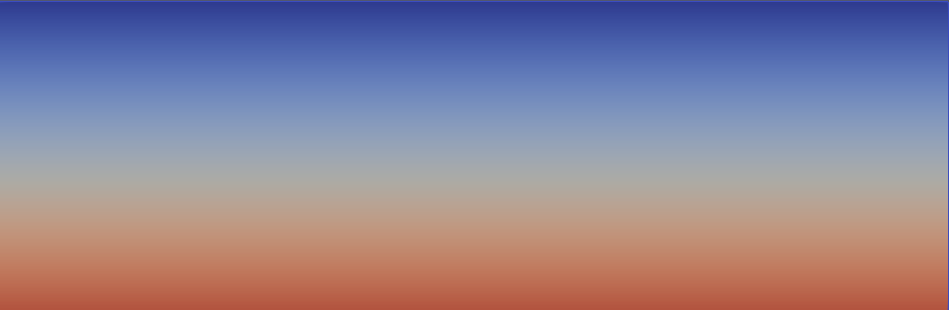
\includegraphics[scale=.3]{animation/fwi_marmousi/fwi_marmousi-00.png}}
%%             {animation/fwi_marmousi/out.avi}
%%     \end{center}
%%   \end{block}

%%   \begin{block}{Mesh evolution (constant mesh):}
%%     \begin{center}
%%       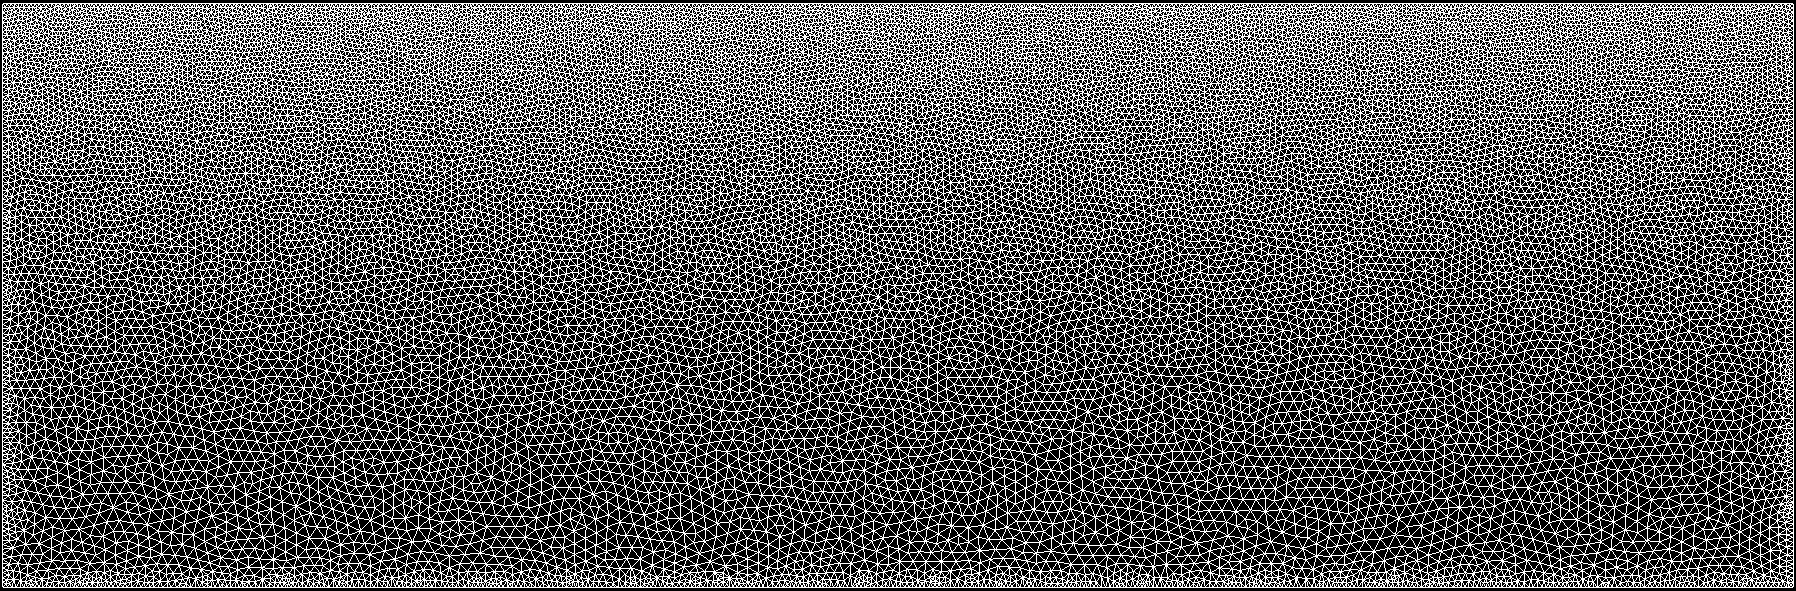
\includegraphics[scale=0.16]{animation/fwi_mesh1_black/fwi_mesh1-00.png}
%%     \end{center}
%%   \end{block}

%% \end{frame}


%% \begin{frame}{Mesh adaptation in FWI workflow}{Motivation:}
%%   \begin{block}{Model evolution:}
%%     \begin{center}
%%       \movie[showcontrols,loop,autostart]
%%             {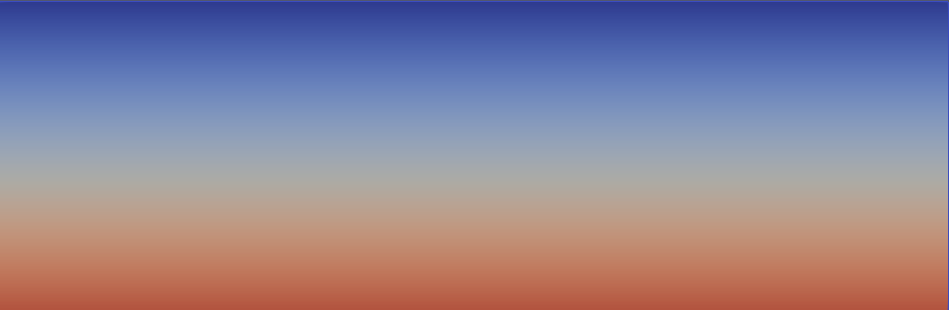
\includegraphics[scale=.3]{animation/fwi_marmousi/fwi_marmousi-00.png}}
%%             {animation/fwi_marmousi/out.avi}
%%     \end{center}
%%   \end{block}

%%   \begin{block}{Mesh evolution (model adaptative):}
%%     \begin{center}
%%             \movie[showcontrols,loop,autostart]
%%             {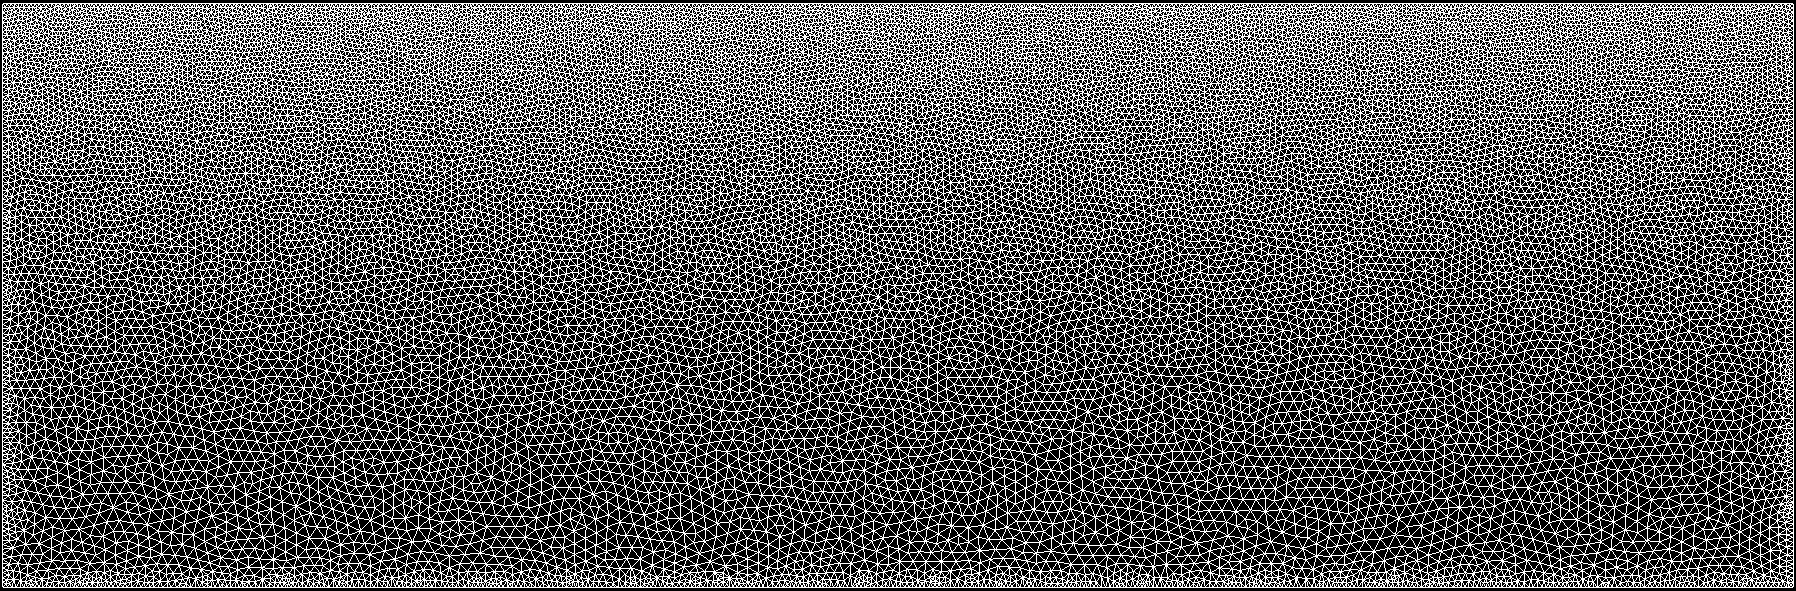
\includegraphics[scale=0.16]{animation/fwi_mesh1_black/fwi_mesh1-00.png}}
%%             {animation/fwi_mesh1_black/out.avi}
%%     \end{center}
%%   \end{block}
%% \end{frame}


%% \begin{frame}{Mesh adaptation in FWI workflow}{Adaptation to the velocity model}
%%   \begin{block}{Model evolution:}
%%     \begin{center}
%%       \movie[showcontrols,loop,autostart]
%%             {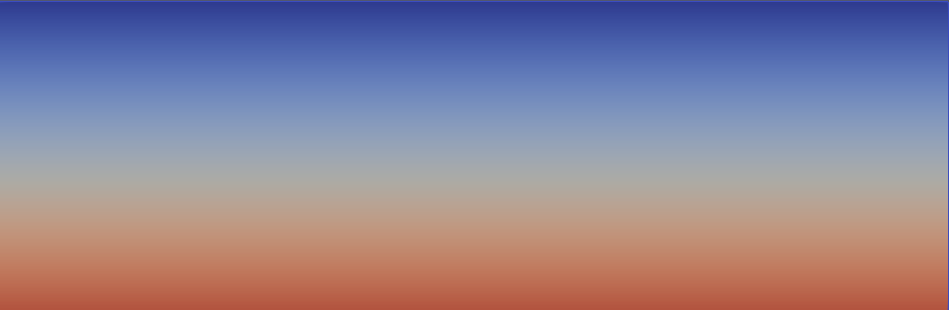
\includegraphics[scale=.3]{animation/fwi_marmousi/fwi_marmousi-00.png}}
%%             {animation/fwi_marmousi/out.avi}
%%     \end{center}
%%   \end{block}

%%   \begin{block}{Mesh evolution (model and frequency adaptative):}
%%     \begin{center}
%%             \movie[showcontrols,loop,autostart]
%%             {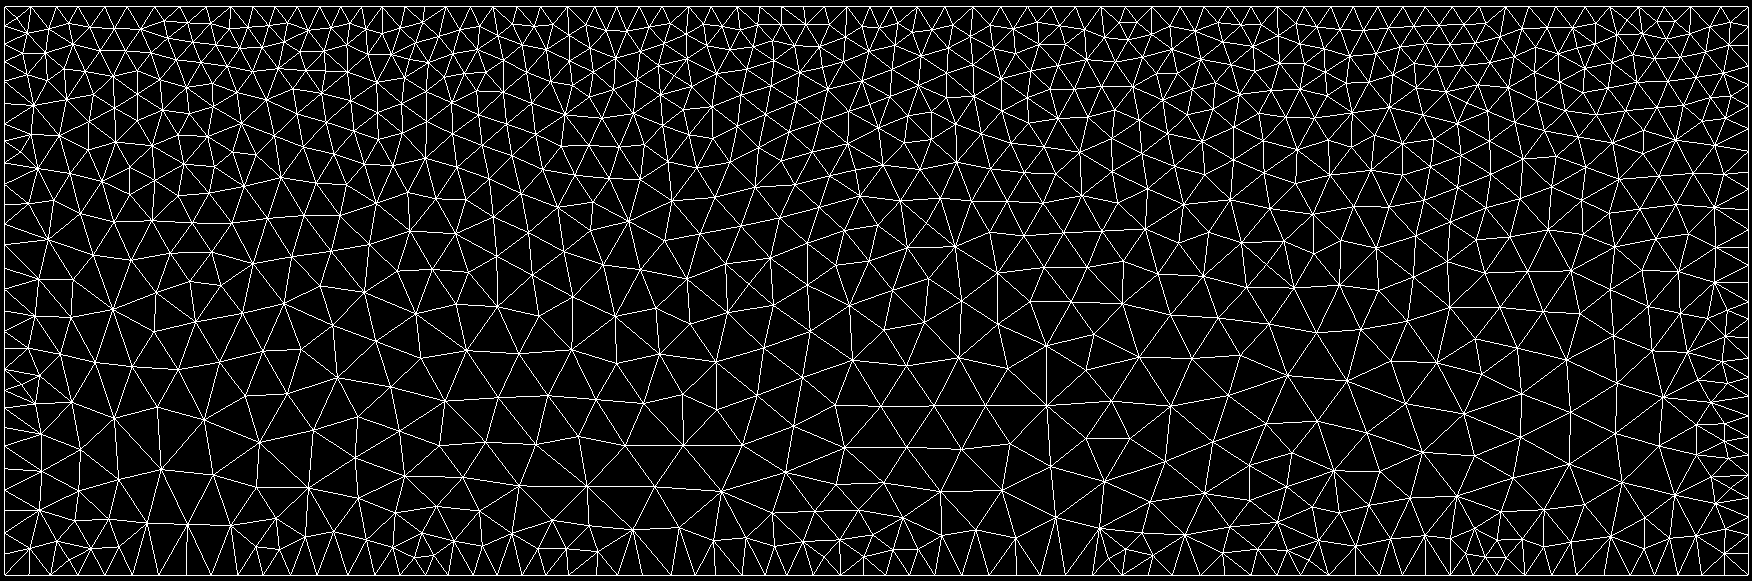
\includegraphics[scale=0.16]{animation/fwi_mesh2/fwi_mesh2-00.png}}
%%             {animation/fwi_mesh2/out.avi}
%%     \end{center}
%%   \end{block}
%% \end{frame}



%% \begin{frame}{Mesh adaptation in FWI workflow}{Introduction}
%%   Why adapting the mesh in the FWI course ?
%%   \vspace{1cm}
%%   \begin{itemize}
%%   \item<2->{Adjust the computational burden}
%%   \item<3->{ Capture appearing structures}
%%   \item<4->{Avoid small cells in high velocity structures (\textbf{relax the CFL condition})}
%%   \item<5->{Enables to choose the mesh according to the frequency range currently reconstructed}
%%   \end{itemize}
%% \end{frame}


%% \begin{frame}{Mesh adaptation in FWI workflow}{Introduction}
%%   How to include mesh adaptation into FWI workflow ?
%% \begin{figure}[!htbp]
%% \centering
%% 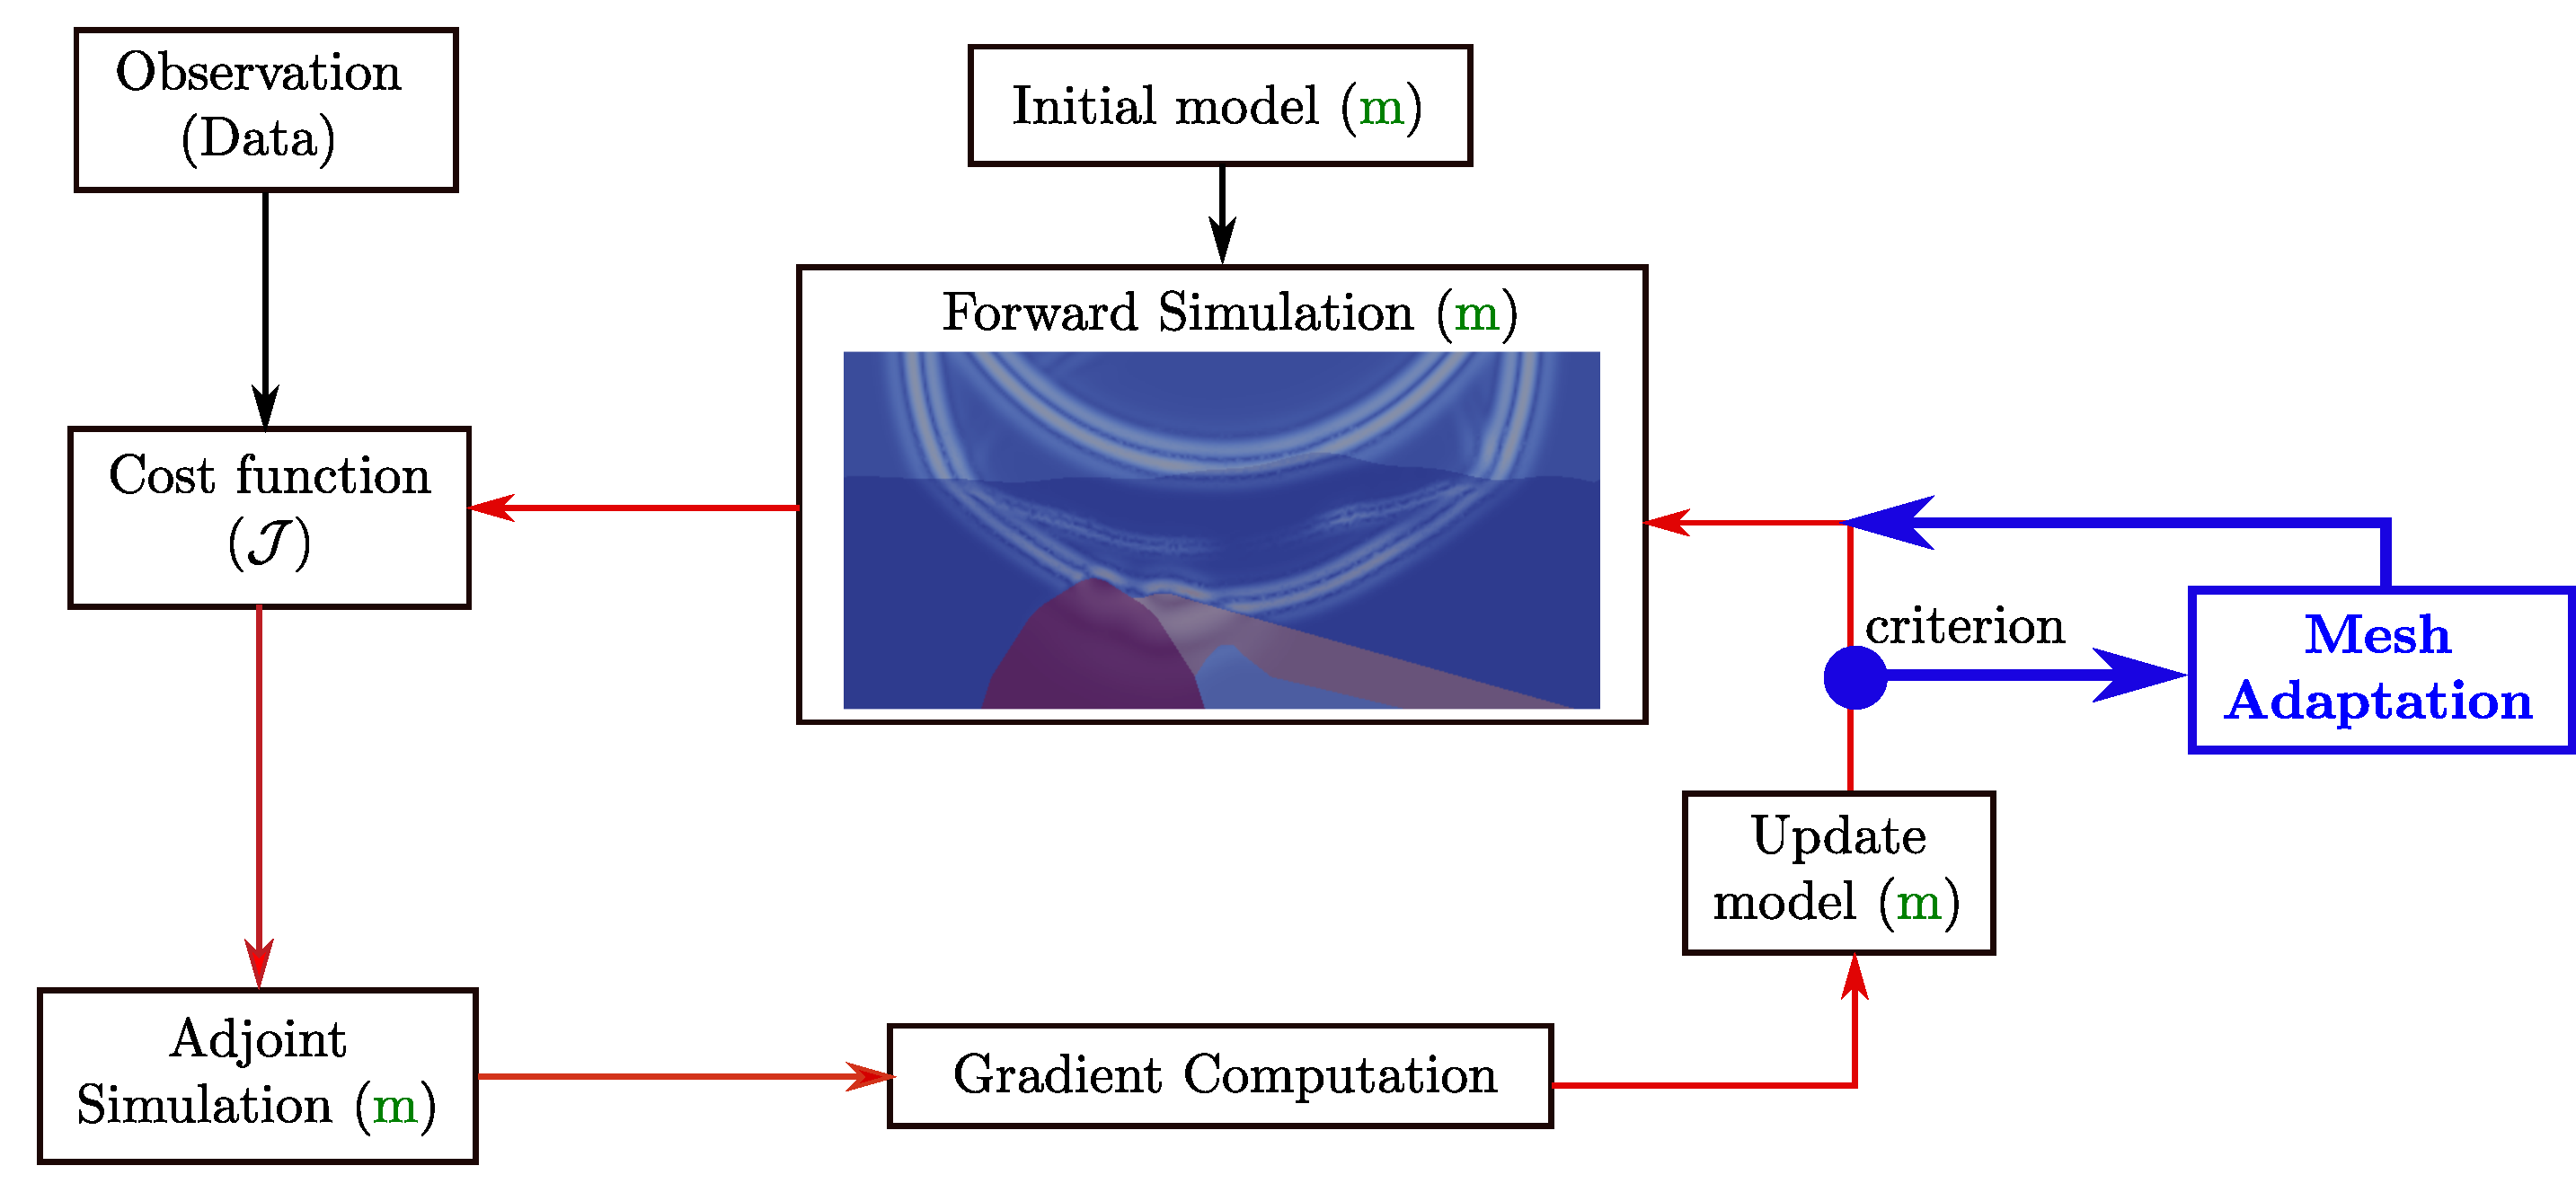
\includegraphics[scale=0.2]{image/fwi_workflow_mesh_adapt.pdf}
%% \caption{FWI workflow extended with mesh adaptation.}
%% \label{fwi_workflow_mesh_extended}
%% \end{figure}
%% \end{frame}

%% \renewcommand{\footnotesize}{\fontsize{7pt}{9pt}\selectfont}
%% \setbeamercovered{invisible}
%% \subsection{Mesh Adaptation}
%% \begin{frame}{Mesh Adaptation}{Definitions}

%%   $\boldsymbol{S^i}$ : solution at the $i^{th}$ iteration |
%%   $\boldsymbol{\Triangles^i}$ : mesh at the $i^{th}$ iteration

%%   \vspace{0.5cm}
%%    \begin{figure}
%%      \begin{tikzpicture}
%%        \node[anchor=south west,inner sep=0] at (0,0) {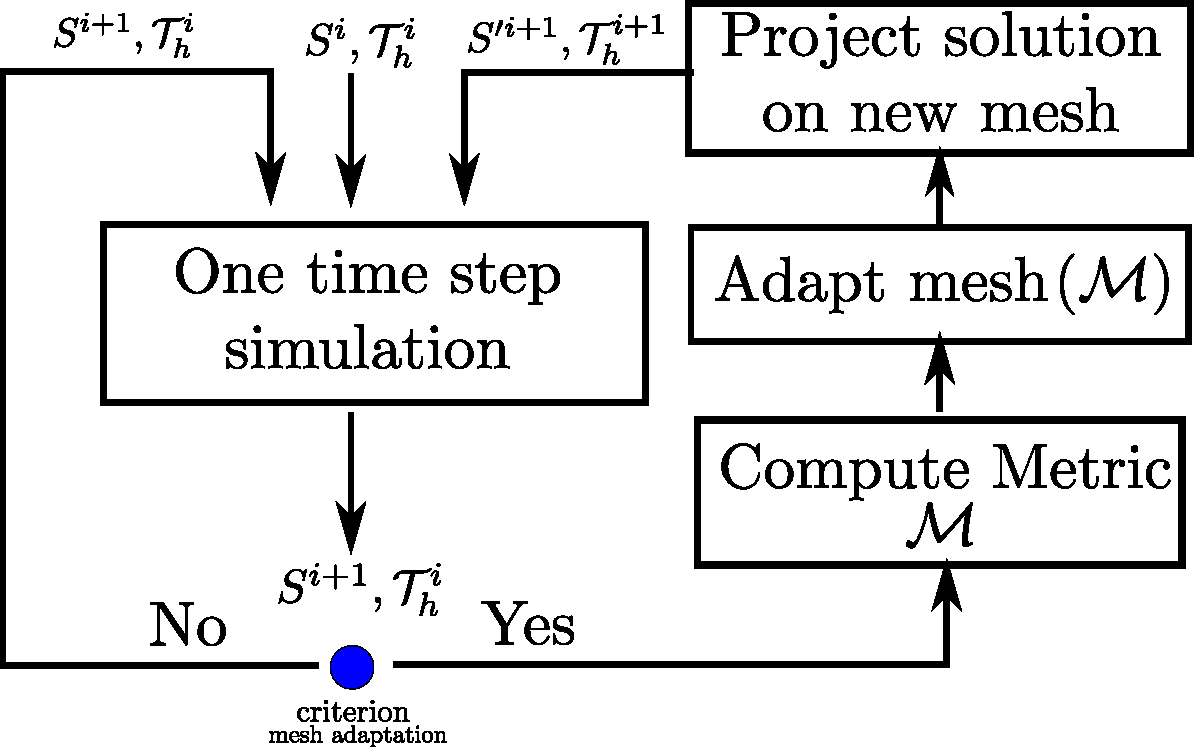
\includegraphics[width=0.8\textheight]{image/mesh_adapt_workflow.pdf}};
%%         \uncover<2->{
%%         \node at (7.6,1.52) {\textbf{\textcolor{blue}{Mshmet \footcite{Mshmet}}}};
%%         \node at (7.6,2.64) {\textbf{\textcolor{red}{MMG \footcite{MMG}}}};
%%           \draw [blue,ultra thick,rounded corners] (3.85,0.95) rectangle (6.7,1.95);
%%           \draw [red,ultra thick,rounded corners] (3.8,2.20) rectangle (6.8,3.0);}
%%         \end{tikzpicture}
%%         \caption{Classical mesh adaptation workflow.}
%%    \end{figure}
%% \end{frame}

%% \begin{frame}{Mesh Adaptation}{Metric field $\metric$}

%%   \begin{block}{Metric definition:}
%%     \small
%%     $\forall P \in \Domain, \boldsymbol{\metric(P)}$ is a \textbf{SPD matrix} of size $\dim \times \dim$.

%%       \begin{empheq}{align}
%%     \forall (P,M) \in \Domain^2, \parallel\vec{PM} \parallel^2_{\metric(P)} &= \langle \vec{PM}, \metric(P) \vec{PM} \rangle \\
%%                               %\parallel\vec{PM} \parallel_{\metric(P)}   &= \sqrt{\vec{PM}^\top \metric(P) \vec{PM}}
%%       \end{empheq}
%%       \end{block}

%%   \uncover<2->{
%%   \begin{block}{Unit ball : Set of point $M$ such that $\parallel \vec{PM} \parallel_{\metric(P)} = 1.$}
%%     \small
%%           \begin{empheq}{align}
%%    \text{In 2D :  } \metric(P) = S \Lambda S^\top\,, \Lambda =  \begin{pmatrix}
%%     \lambda_{1} &\\
%%     & \lambda_2
%%   \end{pmatrix}\,, \lambda_1 \geq \lambda_2 > 0.
%%           \end{empheq}
%%           \begin{multicols}{2}
%%             \begin{figure}[!htbp]
%% \centering
%% 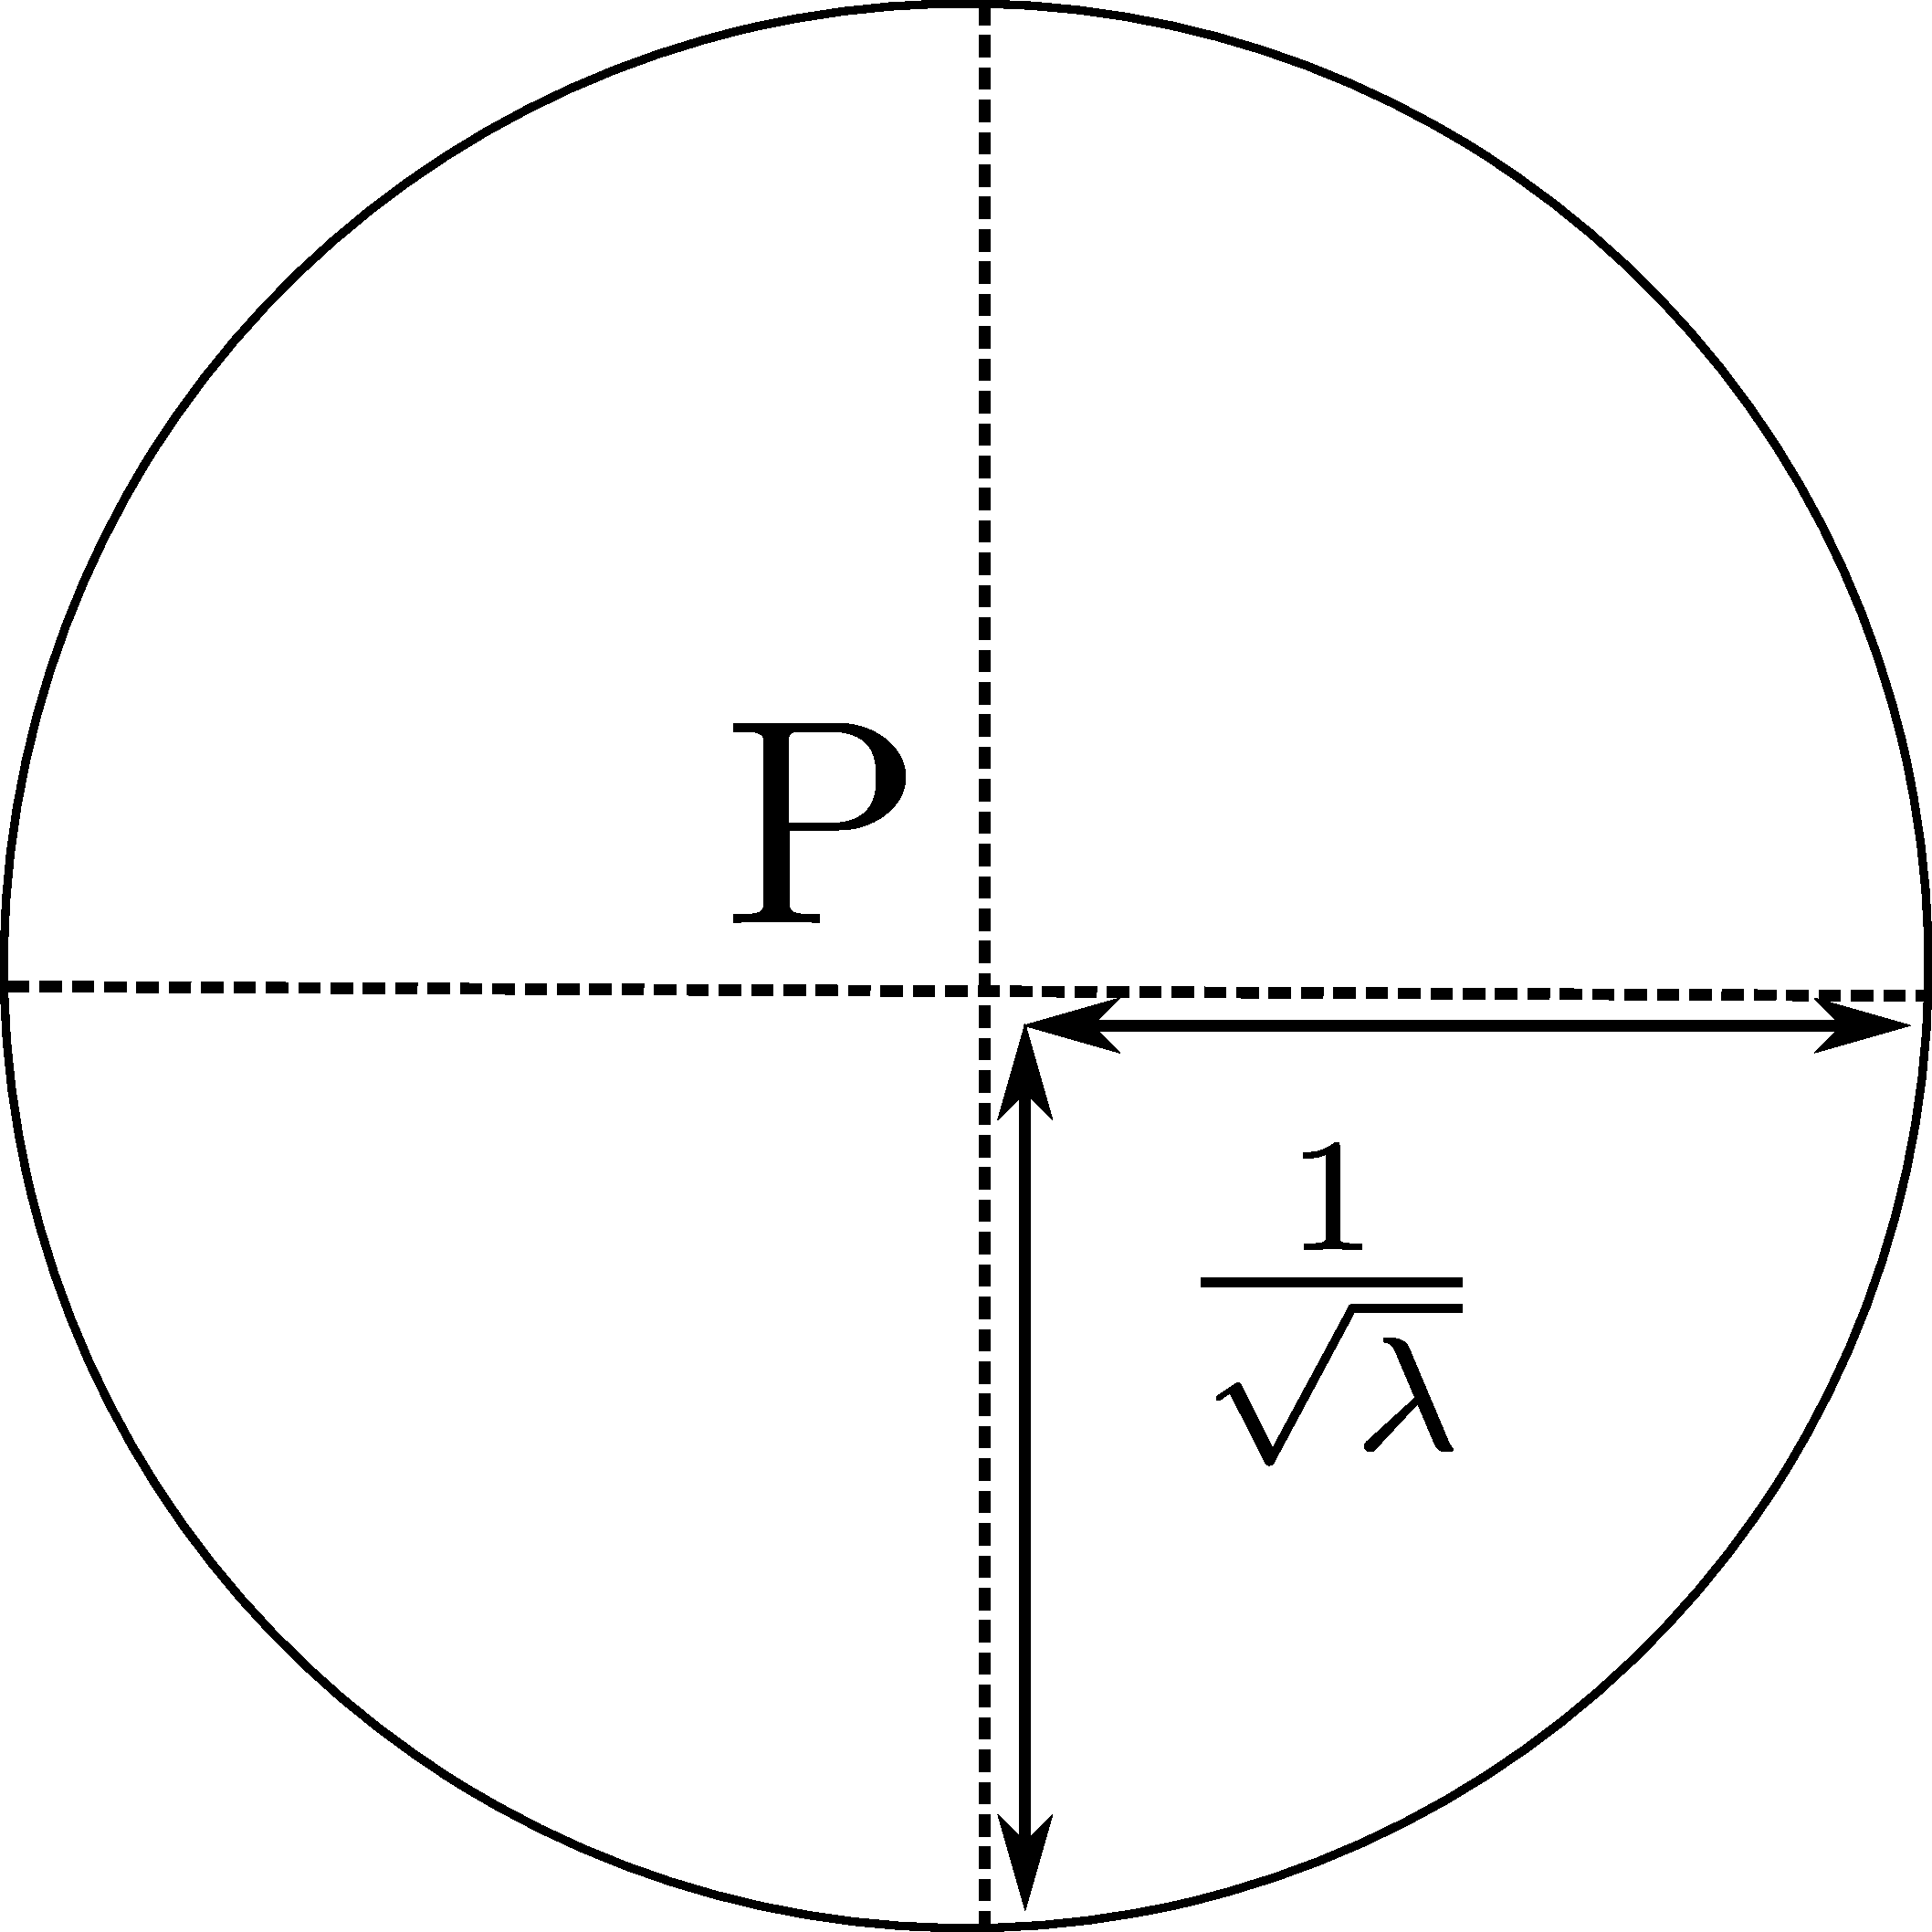
\includegraphics[scale=0.04]{image/ellipse_iso_triangle.pdf}
%% \caption{\tiny{Unit ball $(\lambda_1 = \lambda_2 = \lambda)$}}
%% \label{ellipse_iso_triangle}
%% \end{figure}
%%             \columnbreak
%%            \begin{figure}[!htbp]
%% \centering
%% 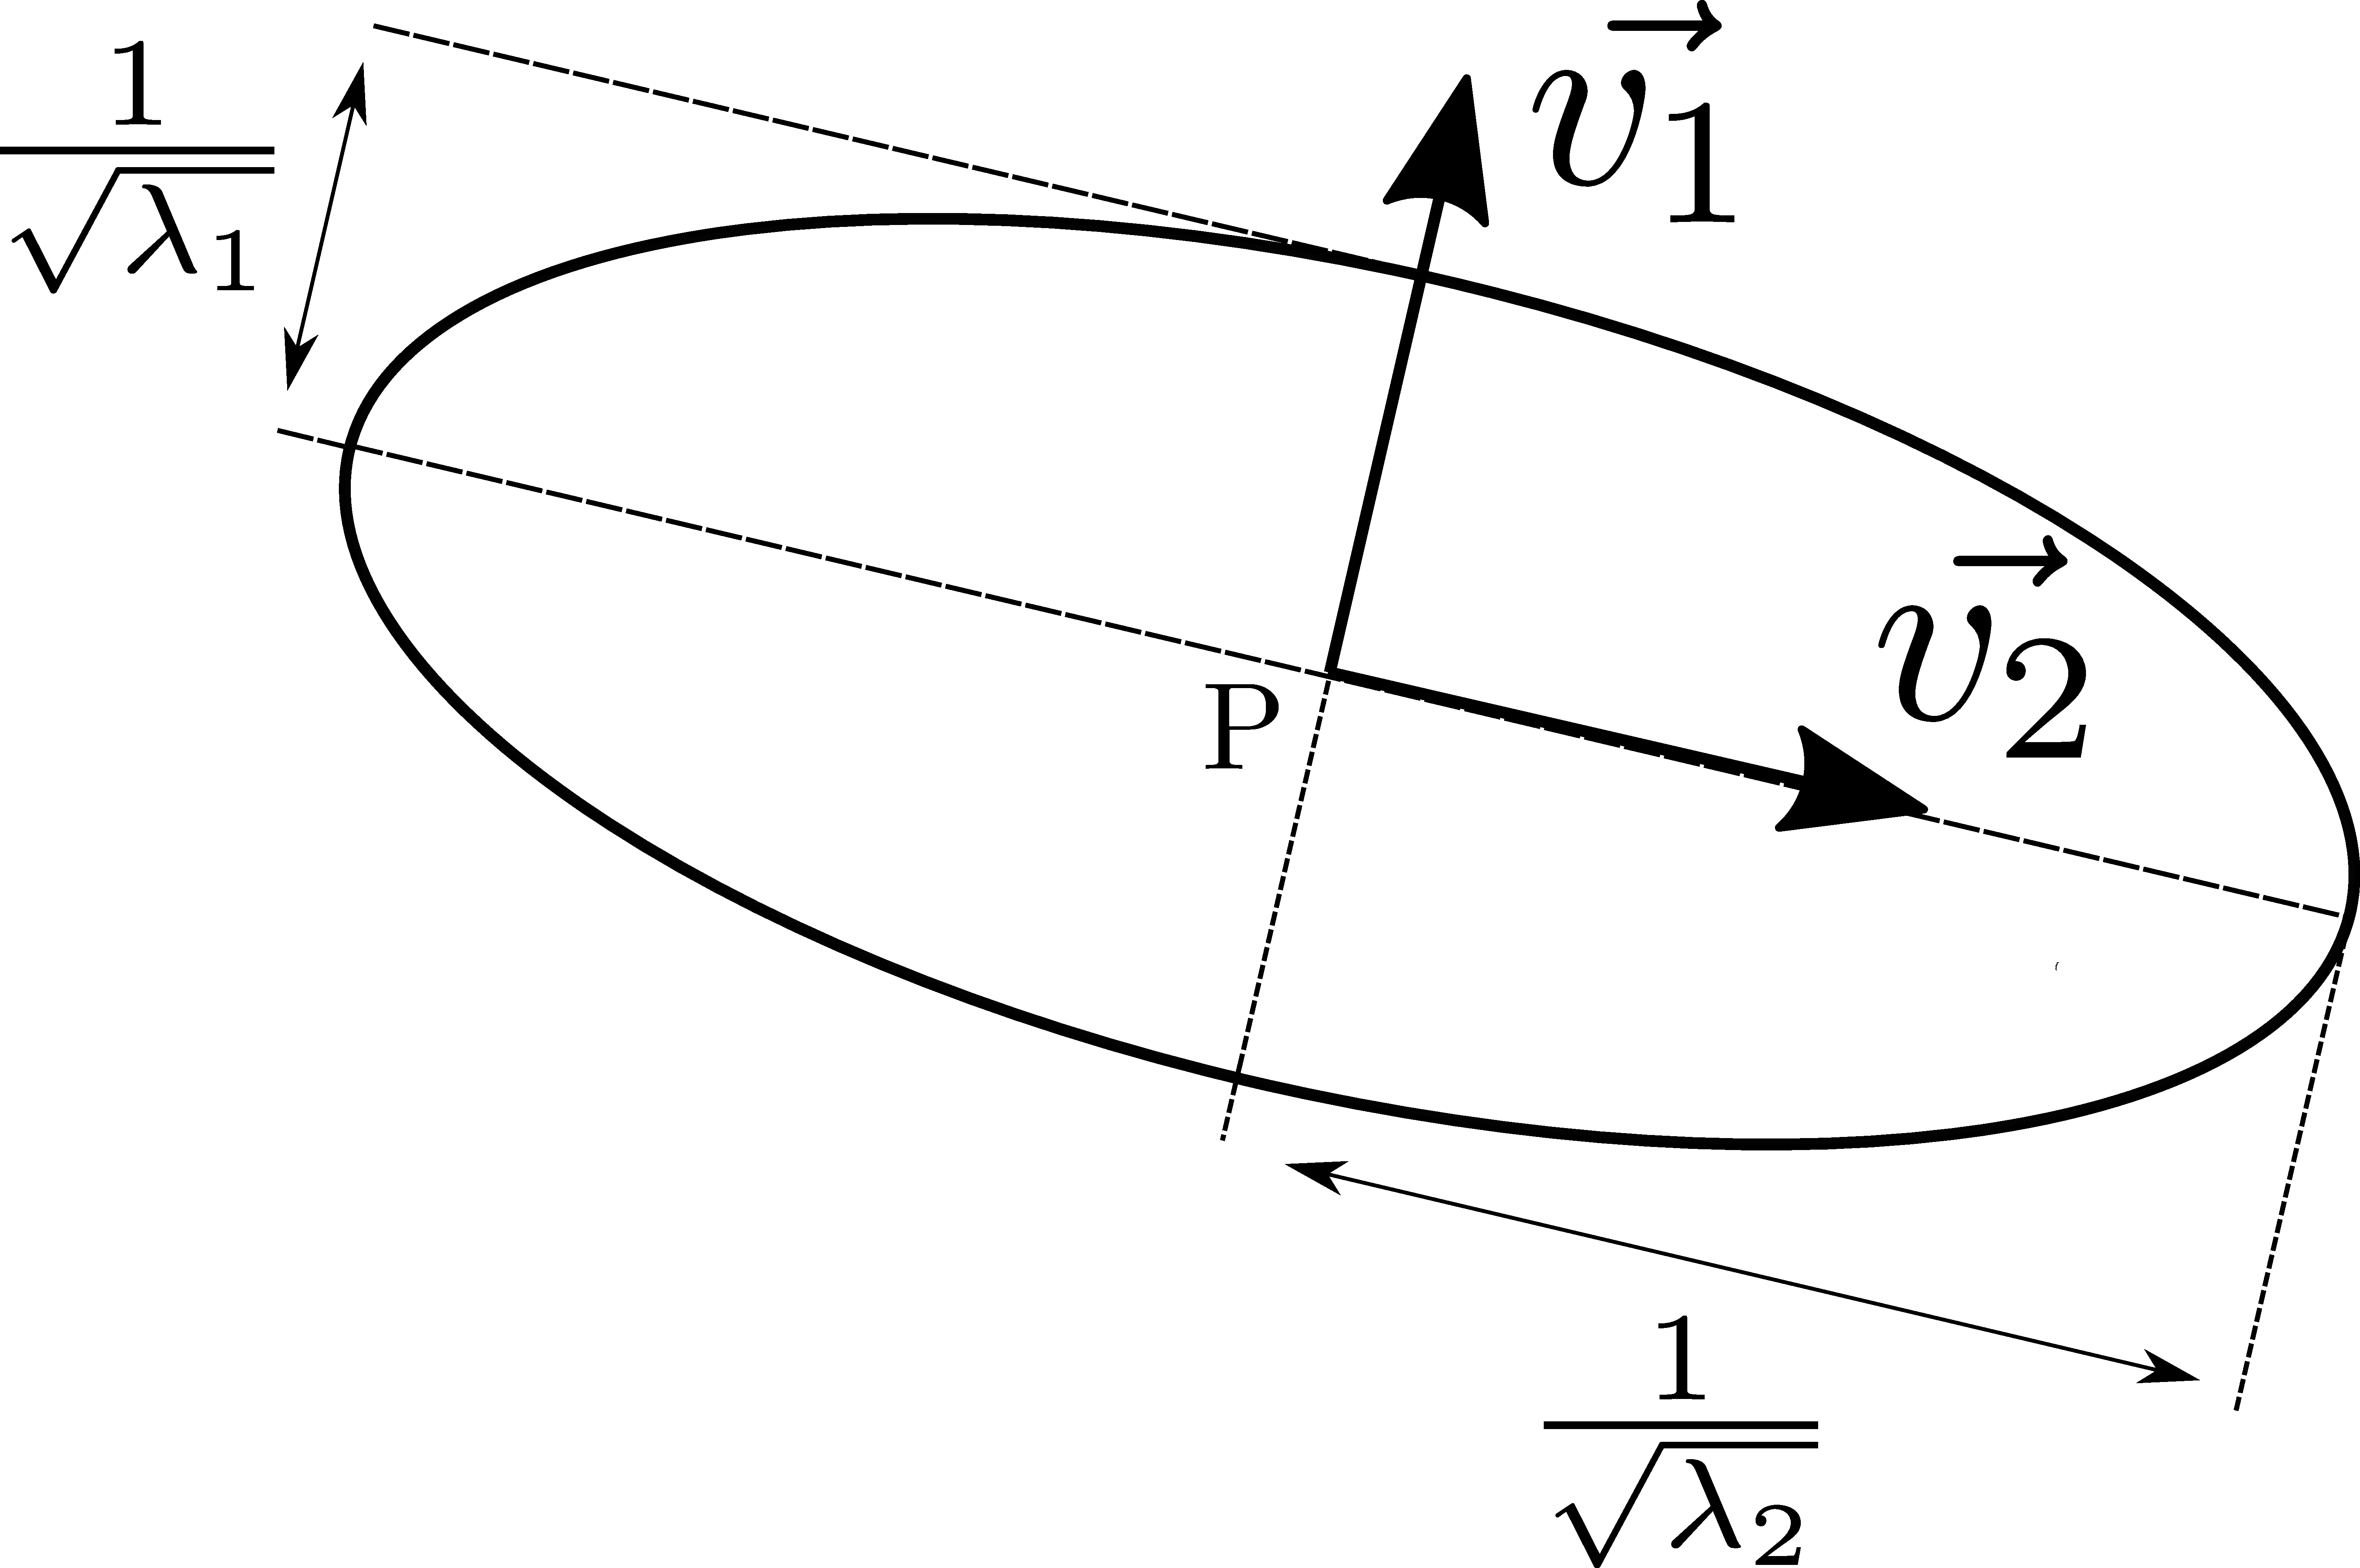
\includegraphics[scale=0.028]{image/ellipse_aniso.pdf}
%% \vspace{-0.5cm}
%% \caption{\tiny{Unit ball $(\lambda_1 >> \lambda_2)$}}
%% \label{ellipse_iso_triangle}
%%      \end{figure}
%%  \end{multicols}
%%   \end{block}
%%   }
%% \end{frame}

%% \begin{frame}{Mesh Adaptation}{Metric field $\metric$}
%%   \small
%%   [P.J. Frey and F. Alauzet]\footcite{freyAnisotropicMeshAdaptation2005}: controle the error on the element $\element$:

%%   \begin{multicols}{2}
%%   \begin{empheq}{align}
%% \exists \, \bar{\metric}(\element)\, / \, \varepsilon_\element = \underset{\overrightarrow{e}\in E_\element}{max} \langle \overrightarrow{e}, \bar{\metric}(\element) \overrightarrow{e} \rangle. \label{error_frey}
%%   \end{empheq}
%%   \columnbreak
%%   \begin{figure}
%%     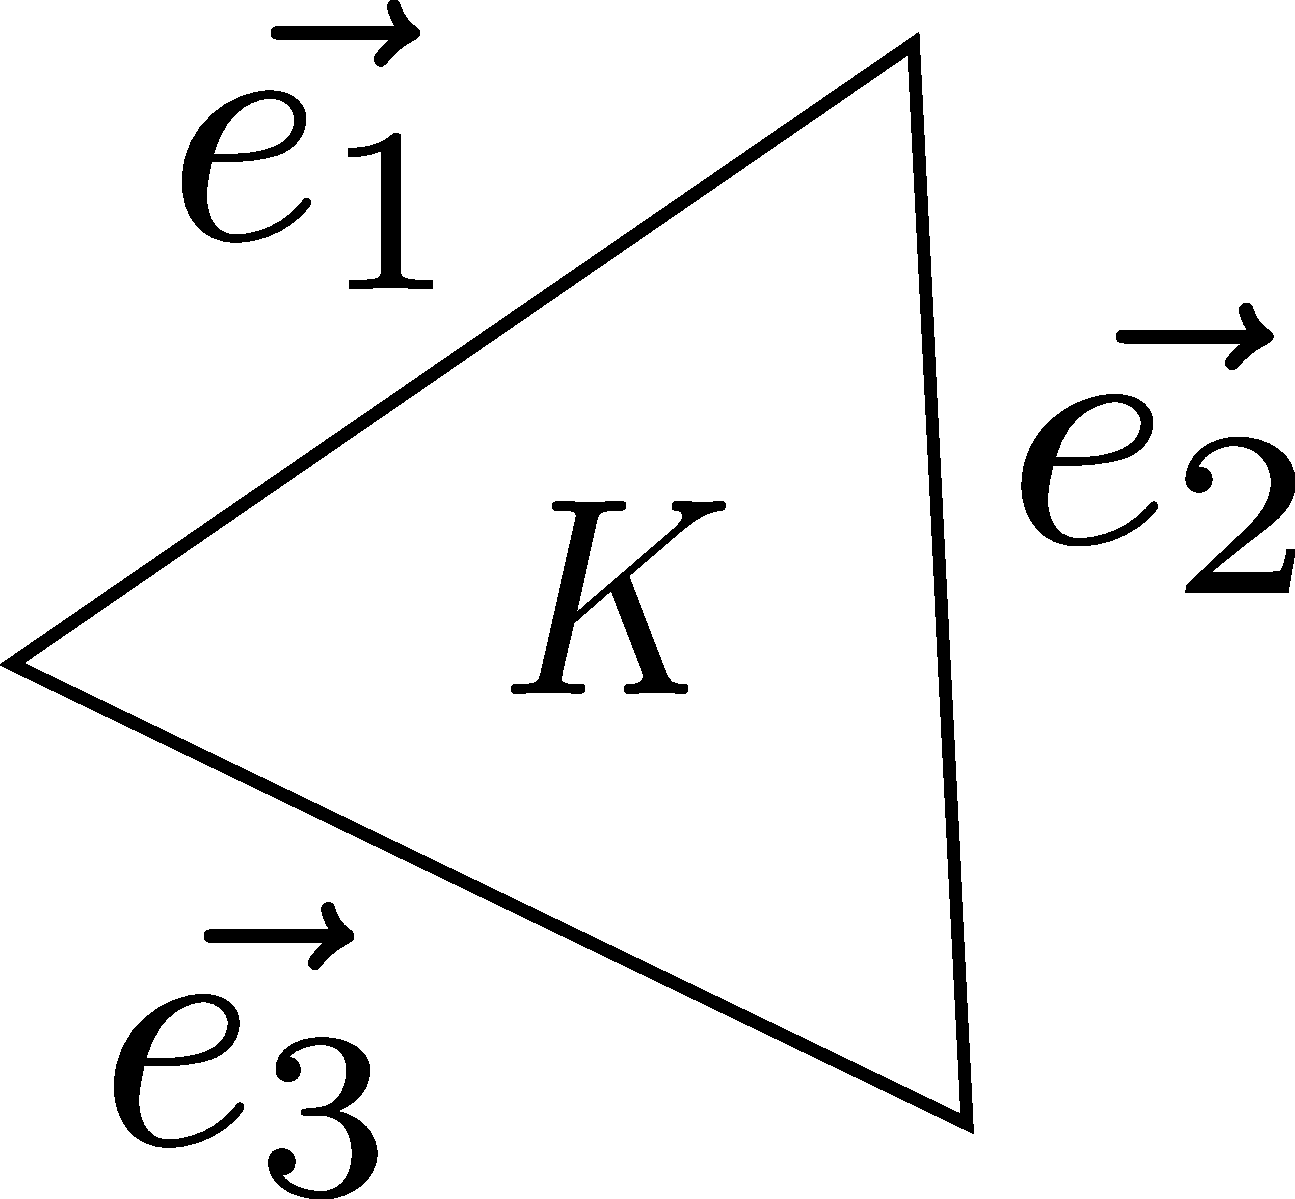
\includegraphics[scale=0.08]{image/triangle_error_frey}
%% %    \caption{Element $K$}
%%     \end{figure}
%%   \end{multicols}

%%   \uncover<2->{
%%   \vspace{-1cm}
%%   \begin{block}{Objective:}
%%     Adapt $\Triangles$ into $\Triangles$' such that:

%%     \begin{empheq}{align}
%%       \varepsilon &= \langle \overrightarrow{e}, \bar{\metric}(\element) \overrightarrow{e} \rangle \,, \qquad \forall \element \in \Triangles'\,, \qquad \forall \overrightarrow{e} \in E_\element. \\
%%             & \qquad \qquad \qquad \text{with:  } \metric = \frac{1}{\varepsilon} \bar{\metric}. \\
%%       1 &= \langle \overrightarrow{e}, \metric(\element) \overrightarrow{e} \rangle \,, \qquad \forall \element \in \Triangles'\,, \qquad \forall \overrightarrow{e} \in E_\element.
%%     \end{empheq}
%%   \end{block}
%% }

%%   \end{frame}

%% %\setbeamercovered{transparent}
%% \begin{frame}{Mesh Adaptation}{Algorithm}

%%   \begin{block}{Distance between $P$ and $M$ according to the metric field $\metric$:}
%%   \begin{empheq}{align}
%% \parallel \overrightarrow{PM} \parallel_\metric =  \int_{0}^{1} \sqrt{ \overrightarrow{PM}^\top  \metric( (1-t)P + tM) \overrightarrow{PM}  } \, dt \,.
%%   \end{empheq}
%%   \end{block}

%%   \begin{enumerate}
%%     \uncover<2->{
%% \item Scan all the edges $\overrightarrow{PM}$ and verify $\parallel \overrightarrow{PM} \parallel_\metric=1$:
%% \begin{itemize}
%% \item{Split the current edge if too long;}
%% \item{Collapse the edge if too short.}
%% \end{itemize}
%%     }
%%     \uncover<3->{
%% \item Check quality of the elements:
%% \begin{itemize}
%% \item Swap edges if "too bad elements";
%% \item{Move points.}
%% \end{itemize}
%%     }
%%     \uncover<3-4>{
%% \begin{tikzpicture}[remember picture,overlay]
%%     \node[xshift=80mm,yshift=-56mm,anchor=north west] at (current page.north west){%
%%     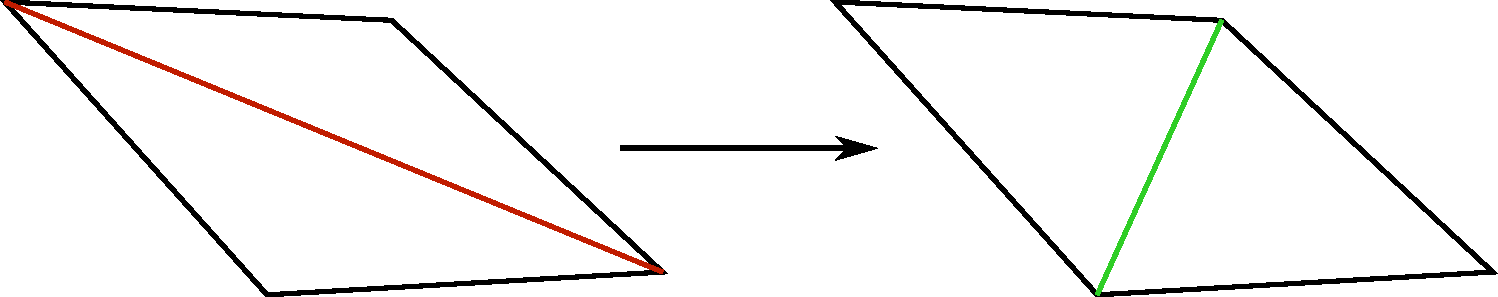
\includegraphics[width=40mm]{image/swap_edge.pdf}};
%% \end{tikzpicture}
%% }
%%     \uncover<4->{
%%       \vspace{-0.5cm}
%%     \item Go to 1. until convergence of the algorithm:
%%       \begin{empheq}{align}
%%         \frac{\sqrt{2}}{2} \le \parallel \overrightarrow{PM} \parallel_\metric \le \sqrt{2}\,.
%%       \end{empheq}
%%       }
%% \end{enumerate}

%% \end{frame}

%% \begin{frame}

%%   \begin{block}{Definition of Isotropic/ Anisotropic cells}
%% \begin{multicols}{2}
%%   \begin{figure}[H]
%% 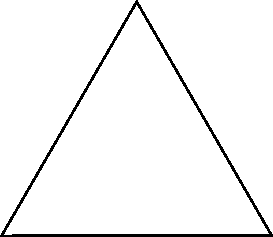
\includegraphics[scale=0.6]{image/isotropic_cell.pdf}
%% \caption{Isotropic cell  ($\lambda_1 = \lambda_2$).}
%% \end{figure}
%% \columnbreak
%% \begin{figure}
%% 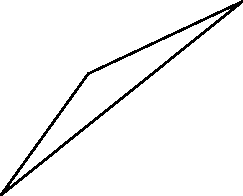
\includegraphics[scale=0.7]{image/anisotropic_cell.pdf}
%% \caption{Anisotropic cell ($\lambda_1 >> \lambda_2$).}
%% \end{figure}
%% \end{multicols}
%% \end{block}
%% \end{frame}


%% \begin{frame}{Define a metric according to the mode parameters}
%%   How to define a metric according to $\smodel^i$ instead of $S^i$ ?
%%   \vspace{0.5cm}
%%   \begin{multicols}{2}
%%     \vspace{-1cm}
%%     \begin{figure}
%%       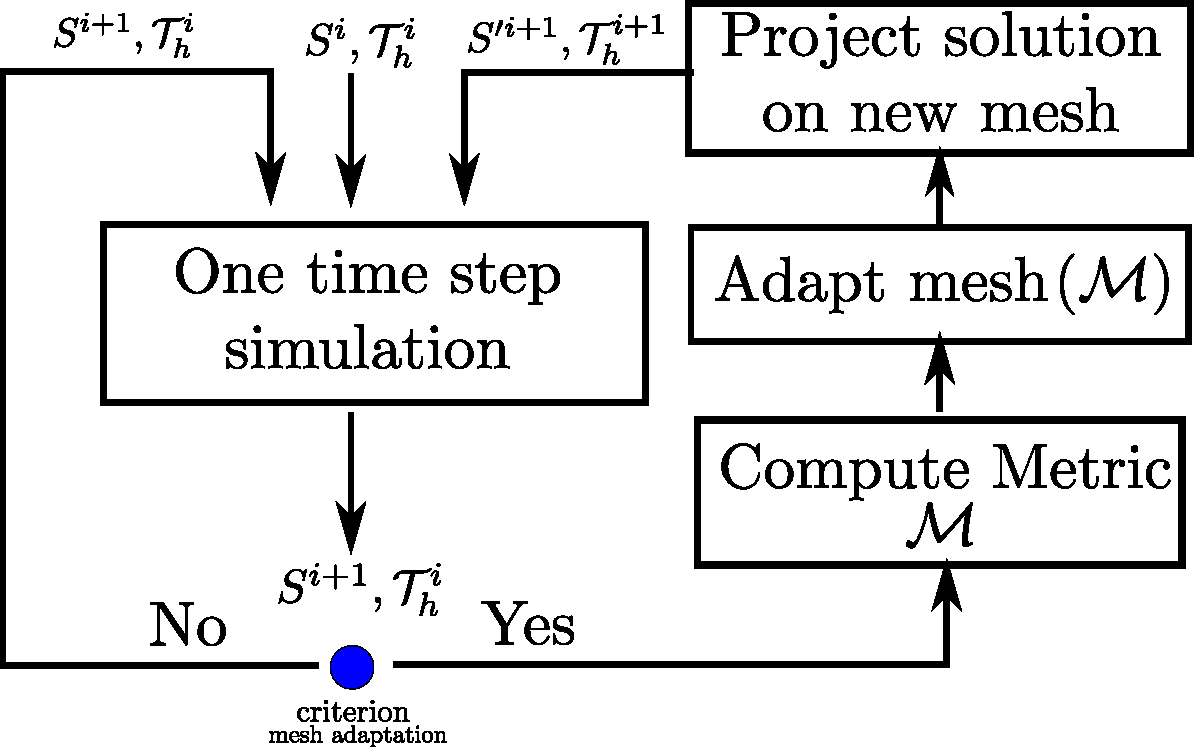
\includegraphics[scale=0.27]{image/mesh_adapt_workflow.pdf}
%%     \end{figure}
%%     \columnbreak
%%         \begin{figure}
%%       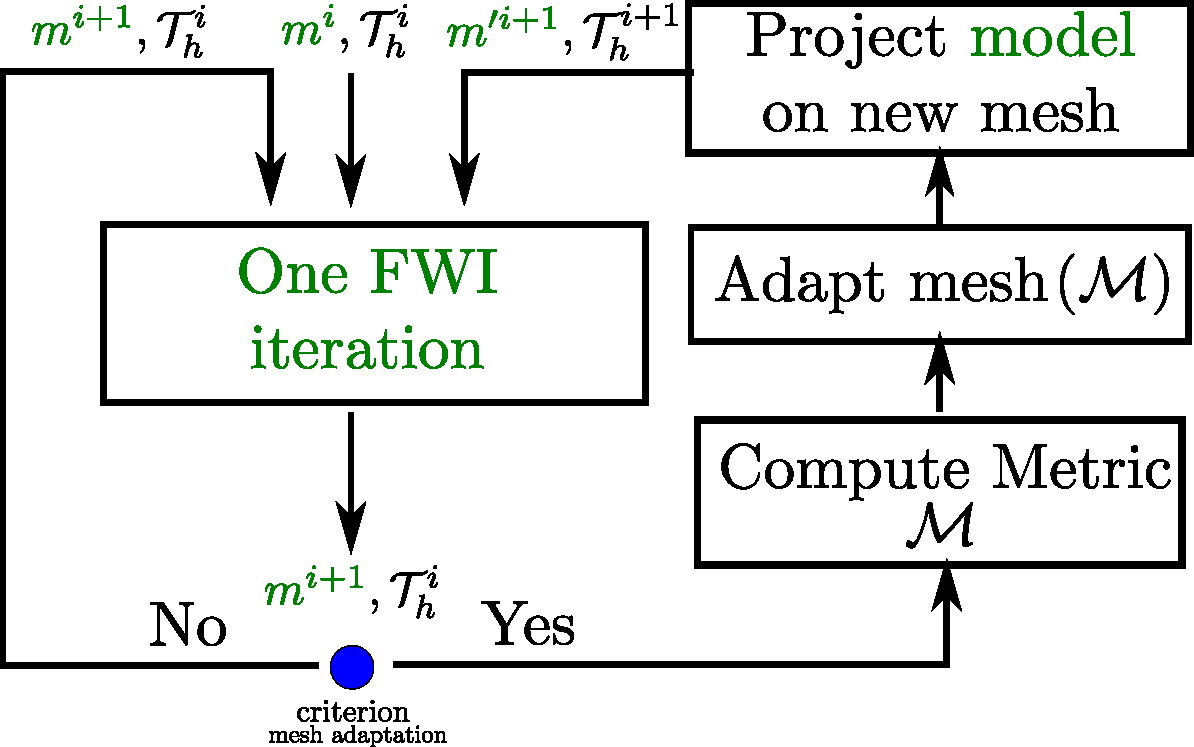
\includegraphics[scale=0.27]{image/mesh_adapt_workflow_fwi.pdf}
%%     \end{figure}
%%      \end{multicols}
%% \end{frame}


%% \begin{frame}
%% \small
%%   No predominant direction $\longrightarrow$ Isotropic metric define by a scalar field (size map ($h(P)$))

%%   In a reference square of size $\lambda \times \lambda$:
%%   \begin{empheq}{align}
%%     \nppw^2  &= \frac{\lambda^2}{a} \frac{(\PolOrder + 1)(\PolOrder + 2)}{2}, \text{  where: } \lambda = \velocity / \fmax \\
%%   \end{empheq}

%%   Isotropic cell hypothesis:
%%   \begin{empheq}{align}
%%     a = \frac{\sqrt{3}}{4} h^2
%%   \end{empheq}

%%   \begin{block}{Heuristic size map formula:}
%%   \begin{empheq}{align}
%%   \forall x \in \Domain, \, \,  h(x)=2\frac{\lambda(x)}{\nppw}\sqrt{\frac{(\PolOrder+1)(\PolOrder+2)}{2\sqrt{3}}} \,.
%%   \end{empheq}
%%   \end{block}
%% \end{frame}


%% \begin{frame}{Numerical assessement of the isotropic size map}
%%   \begin{multicols}{2}
%%     \begin{itemize}
%%     \item 2s simulation
%%     \item 1 source: First order ricker $\fpeak=10$Hz
%%     \item 462 receivers
%%     \item Constant velocity model (to avoid errors from mis-representation of the model)
%%     \item compare numerical traces with analytic traces \footcite{gar6more}
%%     \item for various $\nppw$ values
%%     \end{itemize}
%%     \columnbreak
%%   \begin{figure}[H]
%%   \centering
%%   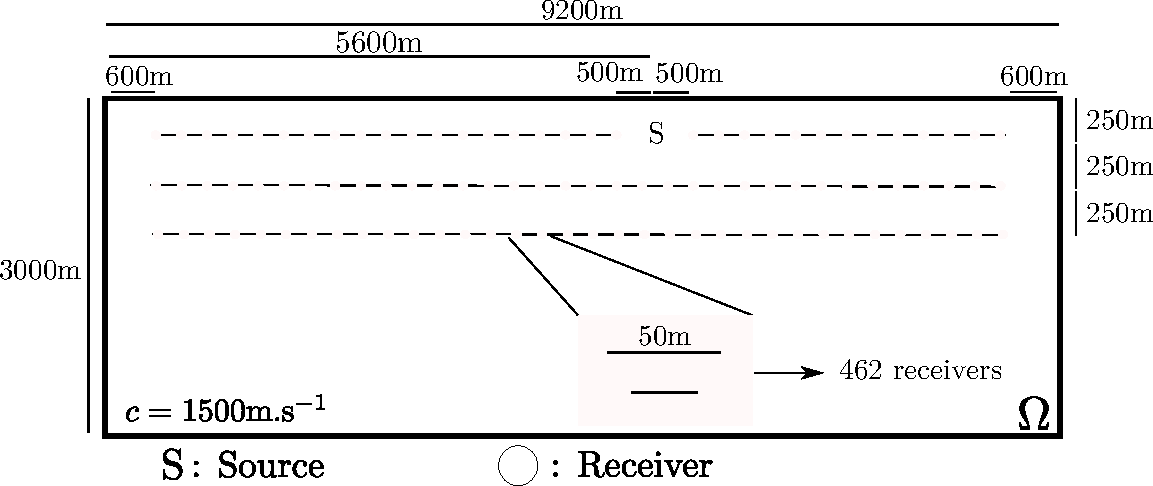
\includegraphics[scale=0.31]{image/precision_test.pdf}
%%   \caption{Experimental setup for the accuracy assessment.}
%%   \label{homogeneous_prec}
%%   \end{figure}
%%   \end{multicols}
%%   \end{frame}

%% \begin{frame}{Error as a function of $\nppw$}
%%   \begin{figure}[H]
%%  \vspace{-0.3cm}
%% \centering
%%  \setlength{\plotwidth}{10cm}
%%     \setlength{\plotheight}{6.0cm}
%%     \begin{tikzpicture}
%%       \begin{axis}[%
%%           width=\plotwidth, height=\plotheight,,
%%           at={(0,0)},scale only axis,separate axis lines,
%%           ymode=log,
%%           xlabel={$\nppw$},
%%           ylabel={error},
%%           grid=both,
%%           grid style={line width=.1pt, draw=gray!10},
%%           major grid style={line width=.2pt,draw=gray!50},
%%           %%   ymode=log,
%%           %yminorticks=true,
%%           %% xmin=0,xmax=35,
%%           %% ymin=0,ymax=1.25,
%%           legend pos=north east
%%           %ymin=0.98,ymax=1.22
%%         ]

%%         %% load current data
%%         %% -----------------
%%         \addplot[color=blue!50!black,mark options={solid}, mark=triangle*,
%%           line width=1pt,
%%           mark size=2pt]
%%         table[x=ppw,y=error]
%%         {graph/mesh_error2.txt};
%%         \addlegendentry{P2}

%%  \addplot[color=red!50!black,mark options={solid}, mark=*,
%%           line width=1pt,
%%           mark size=2pt]
%%         table[x=ppw,y=error]
%%         {graph/mesh_error3.txt};
%%         \addlegendentry{P3}

%%  \addplot[color=green!50!black,mark options={solid}, mark=square*,
%%           line width=1pt,
%%           mark size=2pt]
%%         table[x=ppw,y=error]
%%         {graph/mesh_error4.txt};
%%         \addlegendentry{P4}

%%  \addplot[color=yellow!50!black,mark options={solid}, mark=diamond*,
%%           line width=1pt,
%%           mark size=2pt]
%%         table[x=ppw,y=error]
%%         {graph/mesh_error5.txt};
%%         \addlegendentry{P5}
%%       \end{axis}
%%       \uncover<2->{
%%        \draw [red,ultra thick,rounded corners] (0.0,0.67) -- (10,0.67);}
%%       %% --------------------------------------------------------------------
%%     \end{tikzpicture}
%%     \end{figure}
%% \end{frame}


%% \begin{frame}{Error as a function of the ratio $\lambda/h$}
%%   \begin{figure}[H]
%%     \vspace{-0.3cm}
%% \centering
%%  \setlength{\plotwidth}{10cm}
%%     \setlength{\plotheight}{6.0cm}
%%         \begin{tikzpicture}
%%       \begin{axis}[%
%%           width=\plotwidth, height=\plotheight,,
%%           at={(0,0)},scale only axis,separate axis lines,
%%           ymode=log,
%%           xlabel={$\lambda/h$},
%%           grid=both,
%%           grid style={line width=.1pt, draw=gray!10},
%%           major grid style={line width=.2pt,draw=gray!50},
%%           %%   ymode=log,
%%           %yminorticks=true,
%%           %% xmin=0,xmax=35,
%%           %% ymin=0,ymax=1.25,
%%           legend pos=north east
%%           %ymin=0.98,ymax=1.22
%%         ]

%%         %% load current data
%%         %% -----------------
%%         \addplot[color=blue!50!black,mark options={solid}, mark=triangle*,
%%           line width=1pt,
%%           mark size=2pt]
%%         table[x=ratio,y=error]
%%         {graph/mesh_error2.txt};
%%         \addlegendentry{P2}

%%  \addplot[color=red!50!black,mark options={solid}, mark=*,
%%           line width=1pt,
%%           mark size=2pt]
%%         table[x=ratio,y=error]
%%         {graph/mesh_error3.txt};
%%         \addlegendentry{P3}

%%  \addplot[color=green!50!black,mark options={solid}, mark=square*,
%%           line width=1pt,
%%           mark size=2pt]
%%         table[x=ratio,y=error]
%%         {graph/mesh_error4.txt};
%%         \addlegendentry{P4}

%%  \addplot[color=yellow!50!black,mark options={solid}, mark=diamond*,
%%           line width=1pt,
%%           mark size=2pt]
%%         table[x=ratio,y=error]
%%         {graph/mesh_error5.txt};
%%         \addlegendentry{P5}
%%       \end{axis}
%%       %% --------------------------------------------------------------------
%%       \uncover<2->{
%%       \draw [red,ultra thick,rounded corners] (0.0,0.67) -- (10,0.67);}
%%     \end{tikzpicture}
%%     \end{figure}
%% \end{frame}

%% \begin{frame}{Summary of the experimental criterion}
%%   \small
%%       \hspace{-1cm}
%%   \begin{table}[!htbp]
%%     \begin{tabular}{|l|c|c|c|c|c|}
%%     \hline
%%         \textbf{Polynomial order ($\PolOrder$)} & 2 & 3 & 4 & 5 & 6 \\ \hline
%%         $\boldsymbol{\nppw}$  & 13 & 10 & 10 & 9 & 9 \\ \hline
%%         \textbf{Ratio} $\boldsymbol{\lambda/h}$ & 3.49 & 2.08 & 1.70 & 1.29 & 1.12 \\ \hline
%%         \textbf{Number of Element} & 303283 & 105788 & 69813 & 40012 & 29894 \\ \hline
%%         \textbf{Computational time (s)} & 5230 & 2764 & 1956 & 2017  & 1789\\ \hline
%%     \end{tabular}
%%     \caption{Summary table for 1$\%$ relative error for 2D DG acoustic solver on triangular grid.}
%%     \label{recap_ppw}
%%   \end{table}
%%   \uncover<2->{
%%   \begin{tikzpicture}[remember picture,overlay]
%%     \draw [red,ultra thick,rounded corners] (-1.0,2.1) rectangle (6.3,2.7);
%% %    \node[xshift=80mm,yshift=-56mm,anchor=north west] at (current page.north west){%
%% %    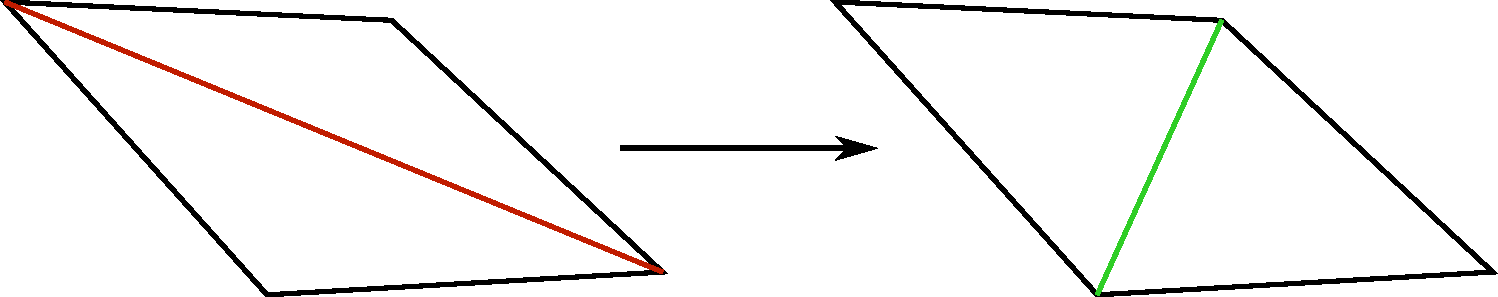
\includegraphics[width=40mm]{image/swap_edge.pdf}};
%%   \end{tikzpicture}
%%   }
%% \end{frame}

%% \begin{frame}{Validation of the isotropic size map}
%%   \begin{block}{}
%%     Polynomial order fixed ($\PolOrder$) $\longrightarrow$ define mesh ($h$-adaptivity)
%%   \end{block}

%%   $\Updownarrow$

%%     \begin{block}{}
%%     Mesh given ($h$) $\longrightarrow$ define the polynomial order ($p$-adaptivity)
%%     \end{block}

%%     \uncover<2->{
%%       \vspace{-0.4cm}
%% \setlength{\modelwidth}{6.5cm}
%% \begin{figure}[!htbp]
%%   \renewcommand{\modelfile}{image/iso22_mesh}
%%      \begin{subfigure}[!htbp]{0.5\textwidth}
%%         \vspace{0.4cm}
%%         \hspace{-0.5cm}
%%          \centering
%%          \begin{tikzpicture}
\pgfmathsetmacro{\xmin} {0.}
\pgfmathsetmacro{\xmax} {9.7}
\pgfmathsetmacro{\zmin} {0.}
\pgfmathsetmacro{\zmax} {2.7}
\pgfmathsetmacro{\zzmax} {3.0}
\pgfmathsetmacro{\xxmax} {10.0}

\begin{axis}[%
width=1.0\modelwidth,
height=0.5\modelwidth,
axis on top, separate axis lines,
xmin=\xmin, xmax=\xxmax, %xlabel={x (km)},
ymin=\zmin, ymax=\zzmax,
yticklabels={},xticklabels={},
y dir=reverse,
point meta min=1.5e3, point meta max=4.6e3,
colorbar/width=2.5mm,
axis x line=top,thick,
axis y line=left,thick,
ylabel style={rotate=-90},
ylabel={$z$},
xlabel={$x$},
ticks = none,
]
\addplot [forget plot] graphics [xmin=\xmin,xmax=\xmax,ymin=\zmin,ymax=\zmax] {{\modelfile}.png};
\end{axis}
\end{tikzpicture}%

%%          \caption{Marmousi refined mesh at the interfaces (12809 elements).}
%%          \label{marmousi_mesh_padapt}
%%      \end{subfigure}
%%      \hspace{-1cm}
%%      \renewcommand{\modelfile}{image/iso22_order}
%%      \renewcommand{\cmapmin}{2}
%%      \renewcommand{\cmapmax}{4}
%%      \begin{subfigure}[!htbp]{0.5\textwidth}
%%         \vspace{-0.3cm}
%%          \centering
%%          \begin{tikzpicture}

\pgfmathsetmacro{\xmin} {0.}
\pgfmathsetmacro{\xmax} {9.7}
\pgfmathsetmacro{\zmin} {0.}
\pgfmathsetmacro{\zmax} {2.7}
\pgfmathsetmacro{\zzmax} {3.0}
\pgfmathsetmacro{\xxmax} {10.0}


\begin{axis}[%
width=1.0\modelwidth,
height=0.5\modelwidth,
axis on top, separate axis lines,
xmin=\xmin, xmax=\xxmax, %xlabel={x (km)},
ymin=\zmin, ymax=\zzmax,
yticklabels={},xticklabels={},
y dir=reverse,
colormap/jet, colorbar,
colorbar style={title=\small{order}},
point meta min=\cmapmin, point meta max=\cmapmax,
colorbar/width=2.5mm,
axis x line=top,thick,
axis y line=left,thick,
ylabel style={rotate=-90},
ylabel={$z$},
xlabel={$x$},
ticks = none,
]
\addplot [forget plot] graphics [xmin=\xmin,xmax=\xmax,ymin=\zmin,ymax=\zmax] {{\modelfile}.png};
\end{axis}
\end{tikzpicture}%

%%          \vspace{-0.9cm}
%%          \caption{$p$-adaptivity map.}
%%          \label{marmousi_order_padapt}
%%      \end{subfigure}

%%   \begin{tikzpicture}[remember picture,overlay]
%%     \draw [red,ultra thick,rounded corners, line width=0.1cm] (-5.5,3.4) rectangle (5.5,4.3);
%% %    \node[xshift=80mm,yshift=-56mm,anchor=north west] at (current page.north west){%
%% %    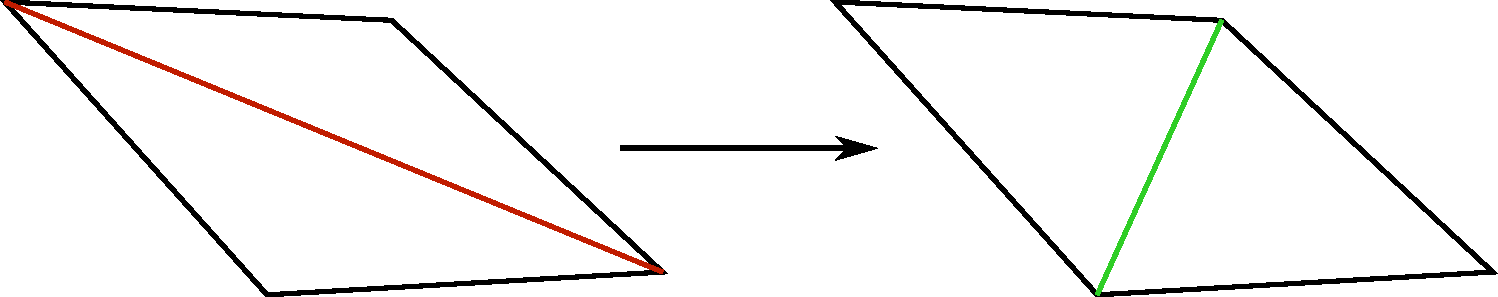
\includegraphics[width=40mm]{image/swap_edge.pdf}};
%%   \end{tikzpicture}
%% \end{figure}
%%      }
%%      \uncover<3->{
%% \vspace{-0.5cm}
%% \begin{table}[!htbp]
%%   \small
%%     \centering
%%     \begin{tabular}{|c|c|c|c|}
%%     \hline
%%          $p$-adaptivity    &  P2   & P3   &  P4   \\ \hline
%%         Number of elements & 1424  & 7981 & 3404   \\ \hline
%%         Pourcentage        & 11\%  &  63\%&  27\%  \\ \hline
%%     \end{tabular}
%%     \caption{Relative error on traces obtained for different $p$-adaptivity strategies.}
%% \end{table}
%% }
%% \end{frame}


%% \begin{frame}[noframenumbering]{Validation of the isotropic size map}
%%   \begin{block}{}
%%     Polynomial order fixed ($\PolOrder$) $\longrightarrow$ define mesh ($h$-adaptivity)
%%   \end{block}

%%   $\Updownarrow$

%%     \begin{block}{}
%%     Mesh given ($h$) $\longrightarrow$ define the polynomial order ($p$-adaptivity)
%%     \end{block}

%%       \vspace{-0.4cm}
%% \setlength{\modelwidth}{6.5cm}
%% \begin{figure}[!htbp]
%%   \renewcommand{\modelfile}{image/iso22_mesh}
%%      \begin{subfigure}[!htbp]{0.5\textwidth}
%%         \vspace{0.4cm}
%%         \hspace{-0.5cm}
%%          \centering
%%          \begin{tikzpicture}
\pgfmathsetmacro{\xmin} {0.}
\pgfmathsetmacro{\xmax} {9.7}
\pgfmathsetmacro{\zmin} {0.}
\pgfmathsetmacro{\zmax} {2.7}
\pgfmathsetmacro{\zzmax} {3.0}
\pgfmathsetmacro{\xxmax} {10.0}

\begin{axis}[%
width=1.0\modelwidth,
height=0.5\modelwidth,
axis on top, separate axis lines,
xmin=\xmin, xmax=\xxmax, %xlabel={x (km)},
ymin=\zmin, ymax=\zzmax,
yticklabels={},xticklabels={},
y dir=reverse,
point meta min=1.5e3, point meta max=4.6e3,
colorbar/width=2.5mm,
axis x line=top,thick,
axis y line=left,thick,
ylabel style={rotate=-90},
ylabel={$z$},
xlabel={$x$},
ticks = none,
]
\addplot [forget plot] graphics [xmin=\xmin,xmax=\xmax,ymin=\zmin,ymax=\zmax] {{\modelfile}.png};
\end{axis}
\end{tikzpicture}%

%%          \caption{Marmousi refined mesh at the interfaces (12809 elements).}
%%          \label{marmousi_mesh_padapt}
%%      \end{subfigure}
%%      \hspace{-1cm}
%%      \renewcommand{\modelfile}{image/iso22_order}
%%      \renewcommand{\cmapmin}{2}
%%      \renewcommand{\cmapmax}{4}
%%      \begin{subfigure}[!htbp]{0.5\textwidth}
%%         \vspace{-0.3cm}
%%          \centering
%%          \begin{tikzpicture}

\pgfmathsetmacro{\xmin} {0.}
\pgfmathsetmacro{\xmax} {9.7}
\pgfmathsetmacro{\zmin} {0.}
\pgfmathsetmacro{\zmax} {2.7}
\pgfmathsetmacro{\zzmax} {3.0}
\pgfmathsetmacro{\xxmax} {10.0}


\begin{axis}[%
width=1.0\modelwidth,
height=0.5\modelwidth,
axis on top, separate axis lines,
xmin=\xmin, xmax=\xxmax, %xlabel={x (km)},
ymin=\zmin, ymax=\zzmax,
yticklabels={},xticklabels={},
y dir=reverse,
colormap/jet, colorbar,
colorbar style={title=\small{order}},
point meta min=\cmapmin, point meta max=\cmapmax,
colorbar/width=2.5mm,
axis x line=top,thick,
axis y line=left,thick,
ylabel style={rotate=-90},
ylabel={$z$},
xlabel={$x$},
ticks = none,
]
\addplot [forget plot] graphics [xmin=\xmin,xmax=\xmax,ymin=\zmin,ymax=\zmax] {{\modelfile}.png};
\end{axis}
\end{tikzpicture}%

%%          \vspace{-0.9cm}
%%          \caption{$p$-adaptivity map.}
%%          \label{marmousi_order_padapt}
%%      \end{subfigure}

%%   \begin{tikzpicture}[remember picture,overlay]
%%     \draw [red,ultra thick,rounded corners, line width=0.1cm] (-5.5,3.4) rectangle (5.5,4.3);
%% %    \node[xshift=80mm,yshift=-56mm,anchor=north west] at (current page.north west){%
%% %    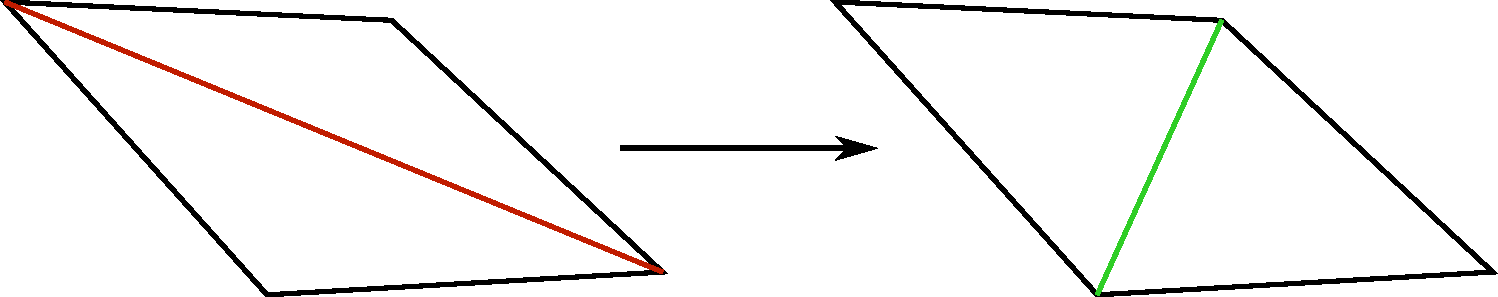
\includegraphics[width=40mm]{image/swap_edge.pdf}};
%%   \end{tikzpicture}
%% \end{figure}

%% \vspace{-1cm}
%% \begin{table}[!htbp]
%%   \small
%%     \centering
%%     \begin{tabular}{|c|c|c|c|c|c|}
%%     \hline
%%          & $p$-adaptivity & Full P2 & Full P3 & Full P4 & Full P5 \\ \hline
%%         L2 relative error & 0.38\%  & 17.40\% & 1.44\% & 0.30\% &  ref. \\ \hline
%%         CPU Time (s) & 815 & 502 & 1122 & 2244 & 3455 \\ \hline
%%     \end{tabular}
%%     \caption{Relative error on traces obtained for different $p$-adaptivity strategies.}
%%     \label{marmousi_padapt_test_error}
%% \end{table}

%% \end{frame}

%% \begin{frame}
%% \begin{figure}%[!htbp]
%% \centering
%% 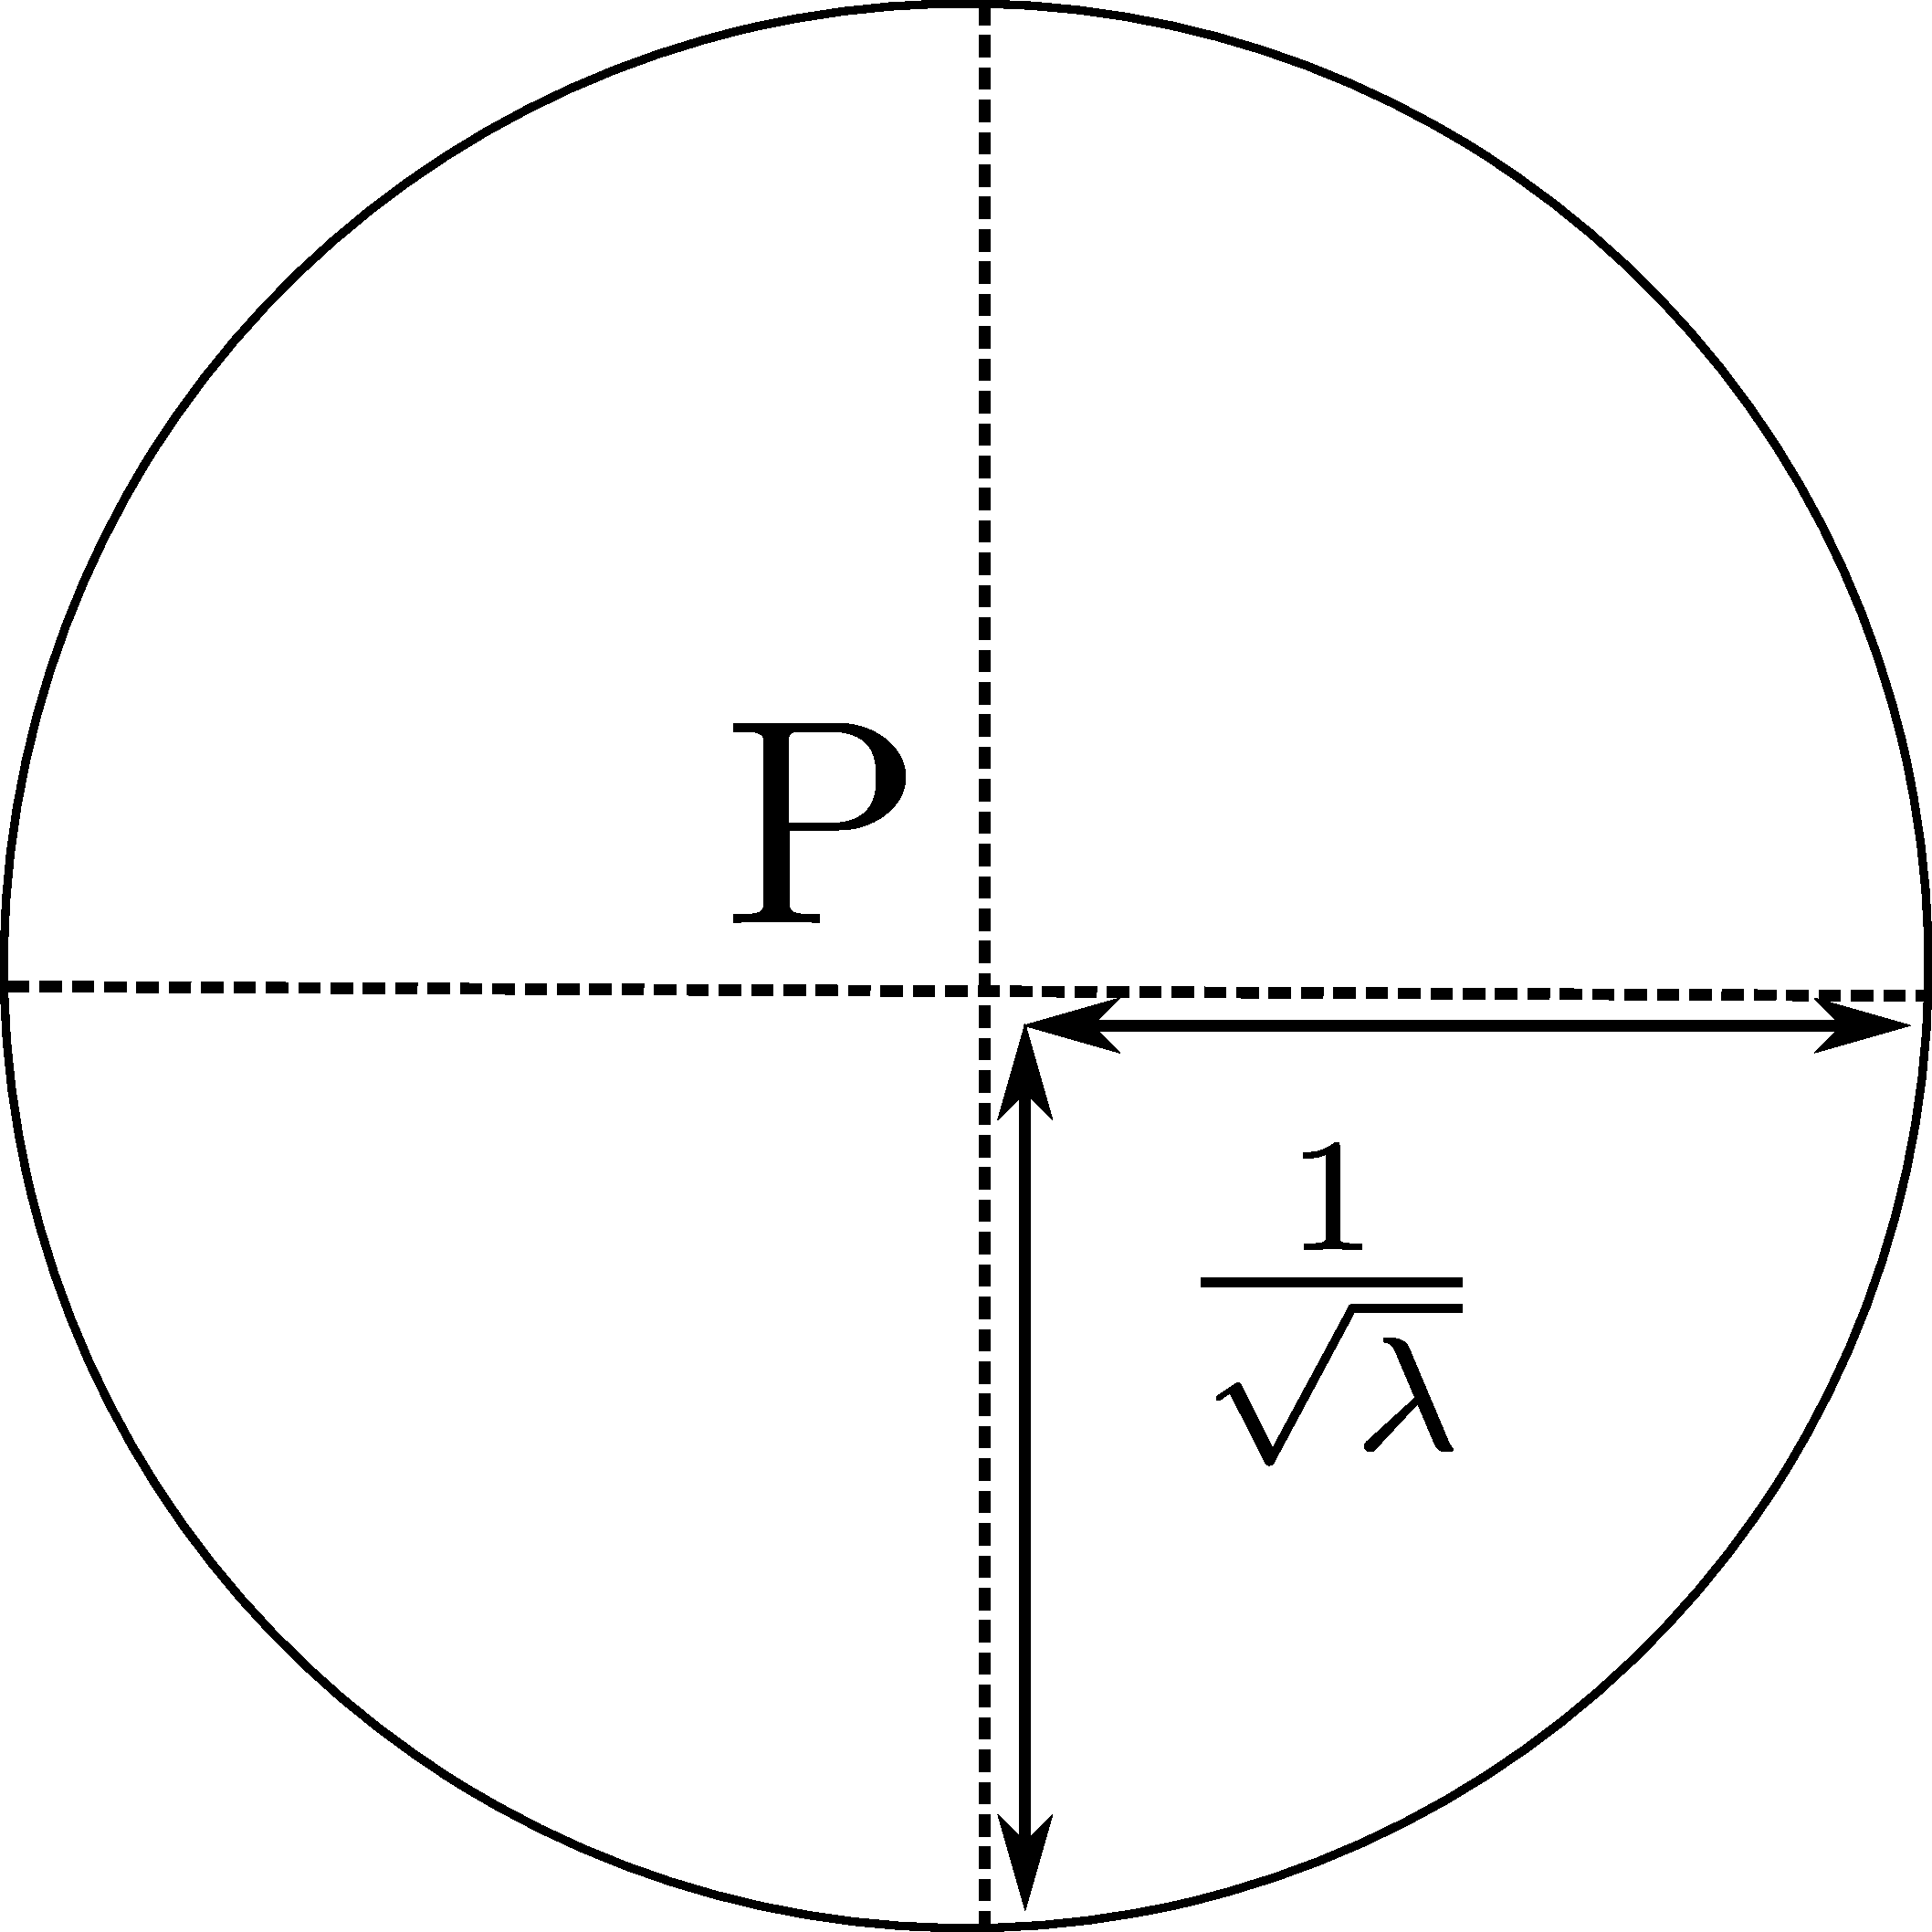
\includegraphics[scale=0.09]{image/ellipse_iso_triangle.pdf}
%% \caption{\tiny{Unit ball centered on $P$ with respect to the distance norm $\parallel.\parallel_{\metric(P)}$ in isotropic case.}}
%% \label{ellipse_iso_triangle}
%% \end{figure}
%% \end{frame}


%%           \begin{multicols}{2}
%% %%             \begin{figure}[!htbp]
%% %% \centering
%% %% 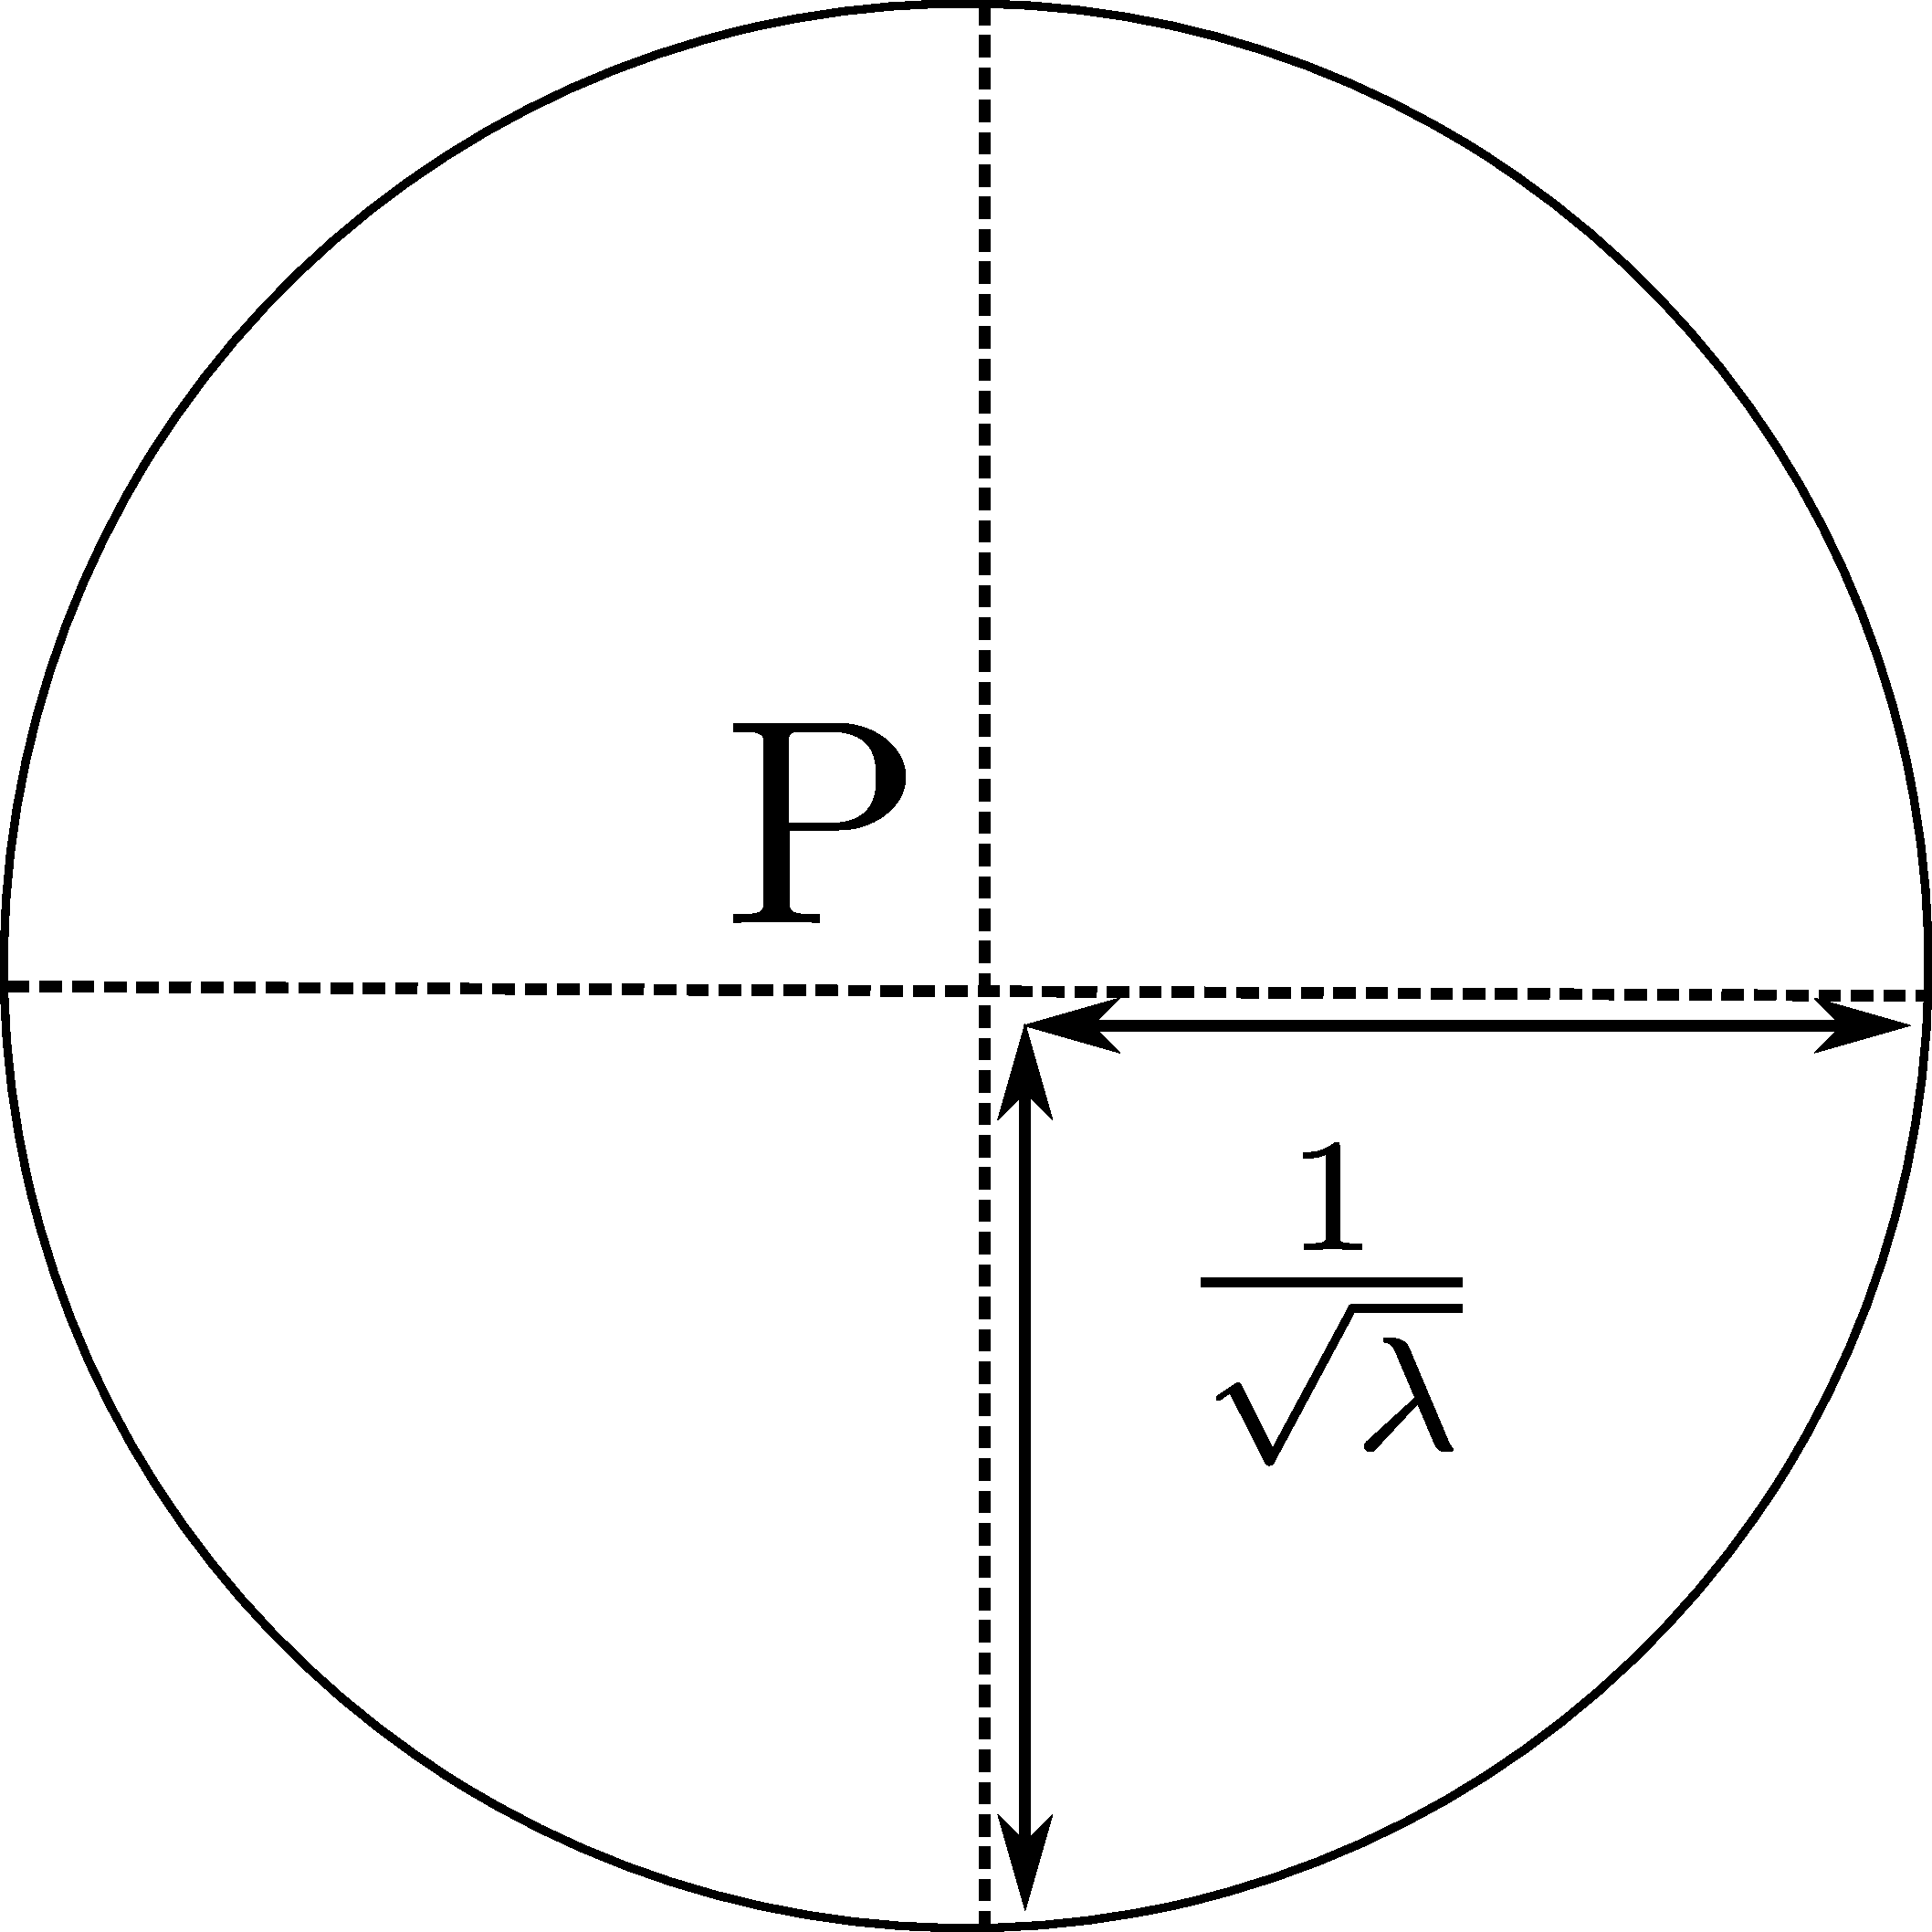
\includegraphics[scale=0.09]{image/ellipse_iso_triangle.pdf}
%% %% \caption{Unit ball centered on $P$ with respect to the distance norm $\parallel.\parallel_{\metric(P)}$ in isotropic case.}
%% %% \label{ellipse_iso_triangle}
%% %% \end{figure}
%% blabla
%%             \columnbreak
%% bloblo
%% %%            \begin{figure}[!htbp]
%% %% \centering
%% %% 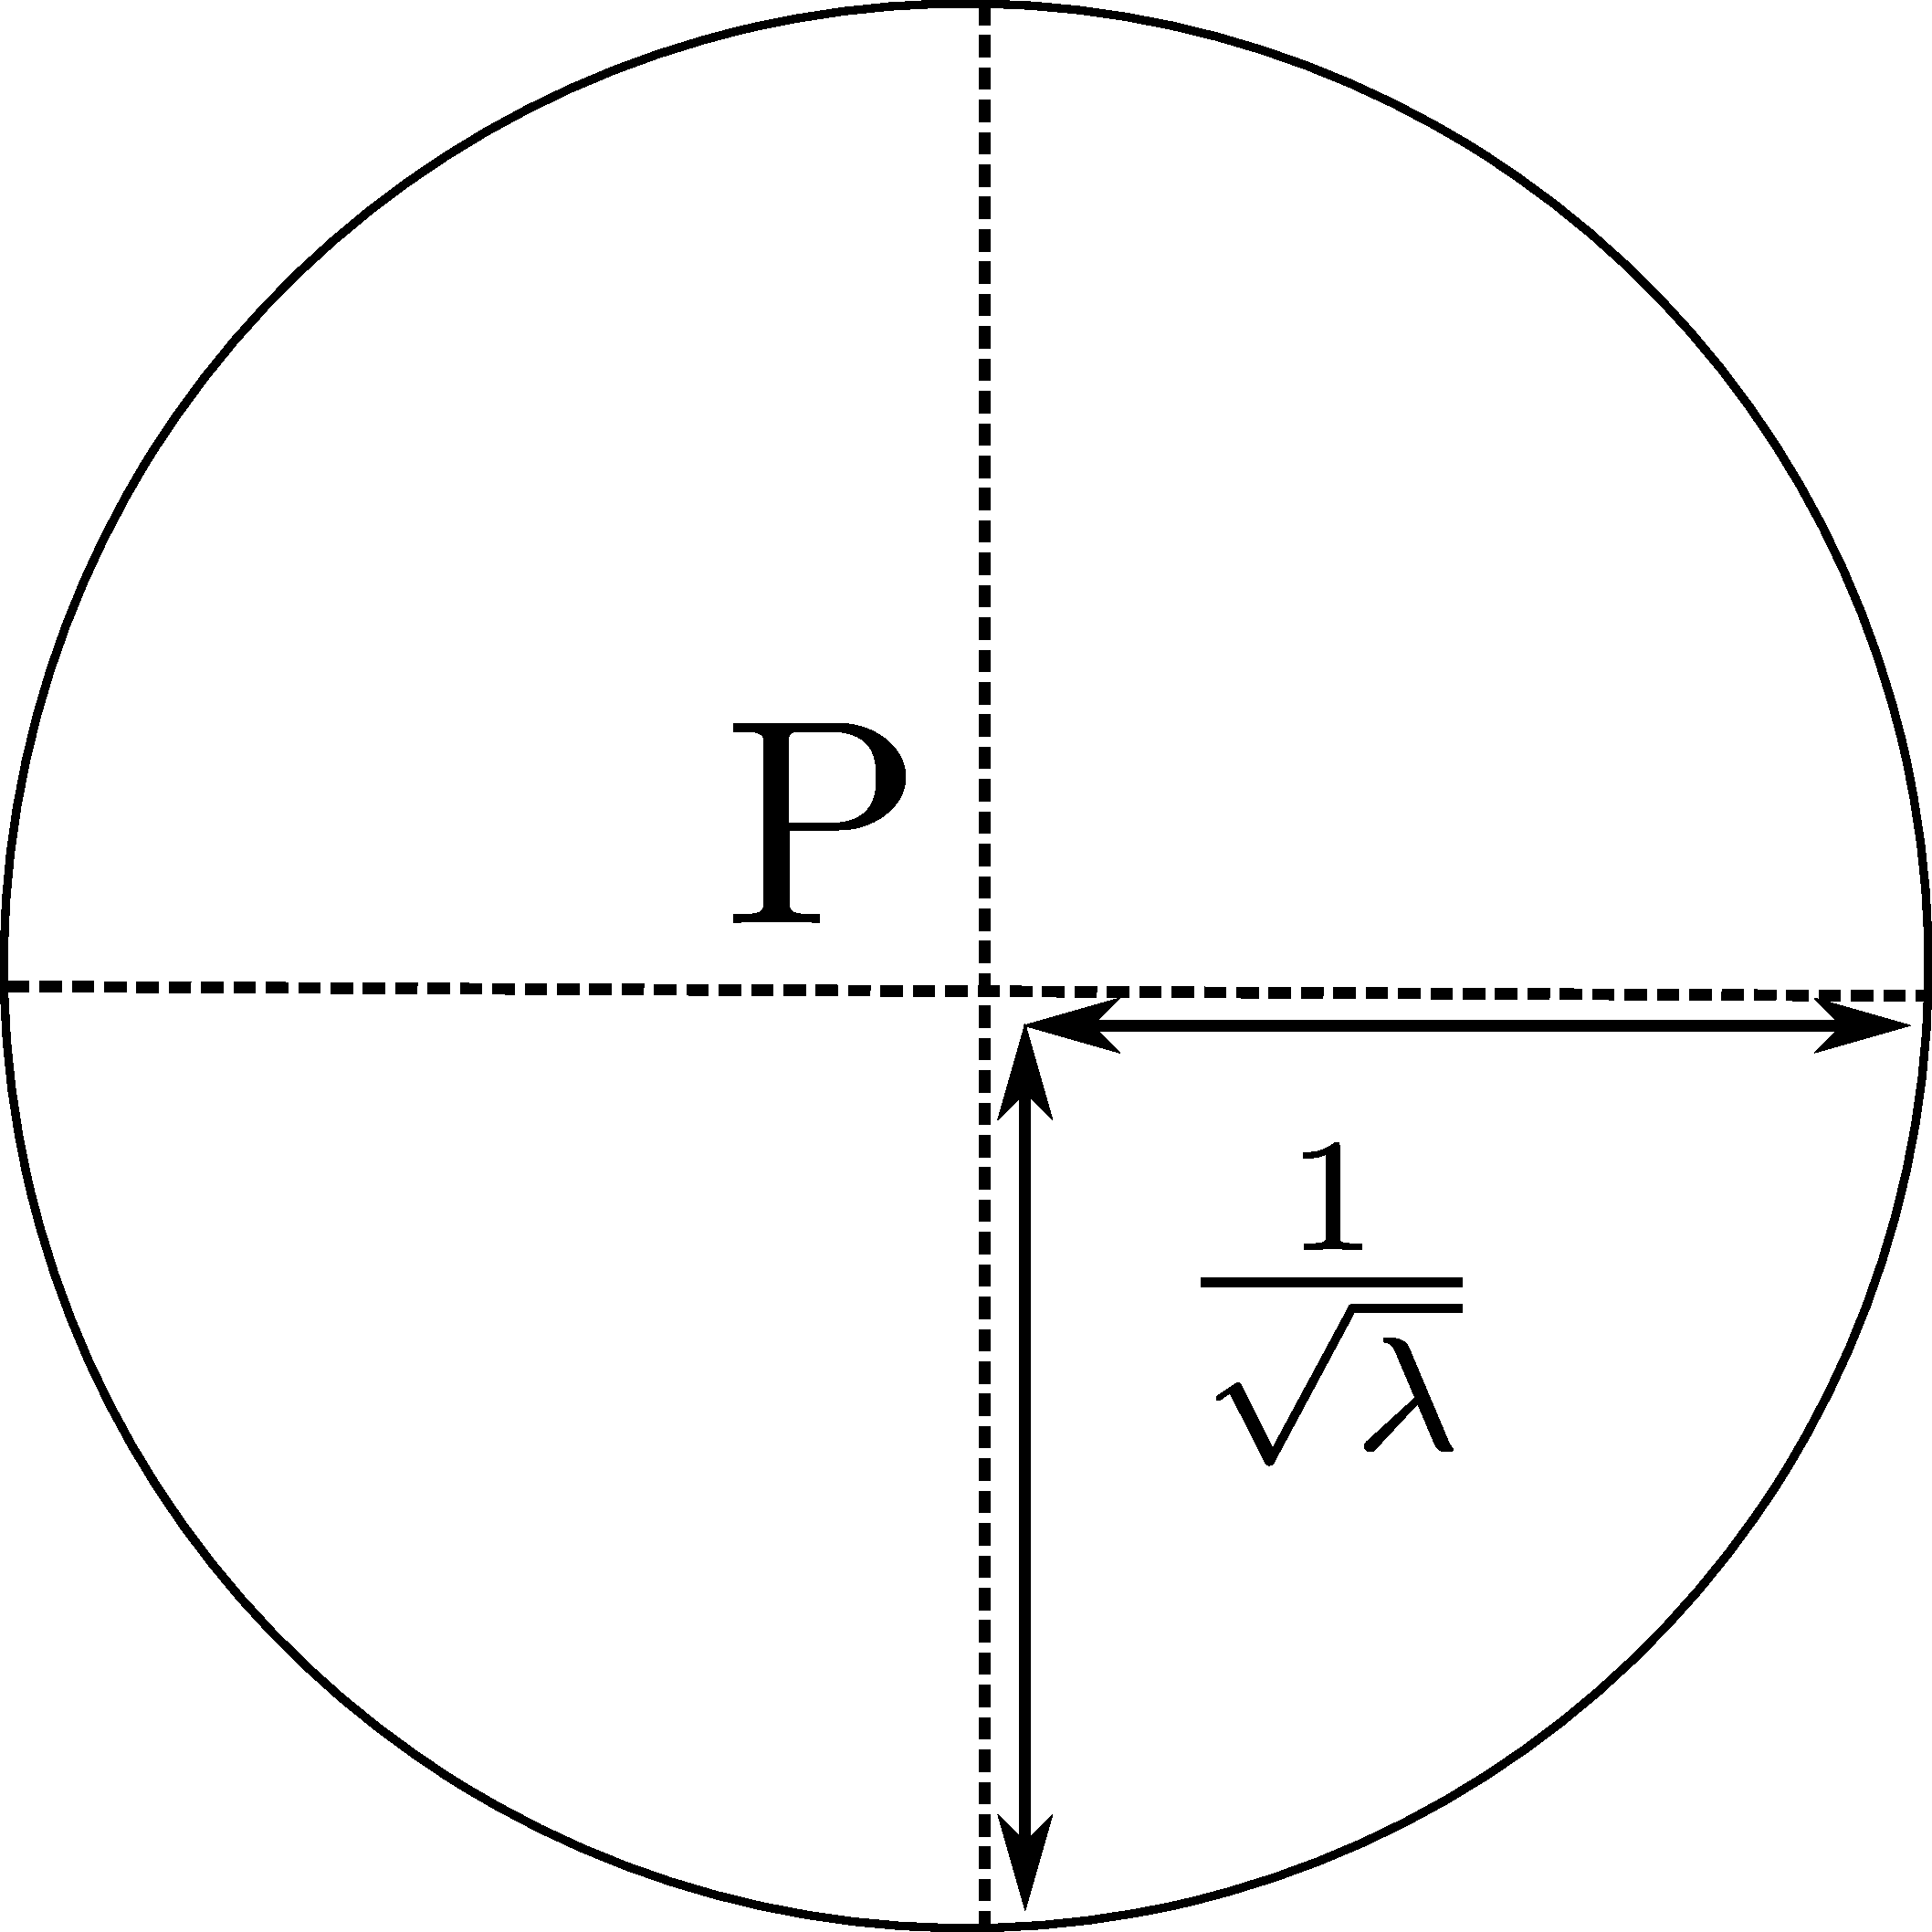
\includegraphics[scale=0.09]{image/ellipse_iso_triangle.pdf}
%% %% \caption{Unit ball centered on $P$ with respect to the distance norm $\parallel.\parallel_{\metric(P)}$ in isotropic case.}
%% %% \label{ellipse_iso_triangle}
%% %% \end{figure}
%%             \end{multicols}



%% {
  \AtBeginSection[]{}
  \section{Time Domain Full Waveform Inversion}
}

\subsection{Seismic Acquisition}

% ============================================
% ====== Frame : Seismic Acquisition  ========
% ============================================
\begin{frame}{Seismic Acquisition}


  \begin{figure}
    \def\svgwidth{1.05\linewidth}
    \input{images/intro_1.pdf_tex}
  \end{figure}

\end{frame}

\begin{frame}[noframenumbering]{Seismic Acquisition}


  \begin{figure}
    \def\svgwidth{1.05\linewidth}
    \input{images/intro_2.pdf_tex}
  \end{figure}

\end{frame}

\newcommand\hideit[1]{%
  \only<0| handout:1>{\mbox{}}%
  \invisible<0| handout:1>{#1}}







% ============================================
% ====== Frame : FWI Workflow 1       ========
% ============================================
\subsection{FWI Workflow}

\begin{frame}{FWI Workflow}
  \begin{columns}
    \column{\dimexpr\paperwidth-10pt}
    \begin{figure}
      \def\svgwidth{1.0\linewidth}
      \input{images/data.pdf_tex}
    \end{figure}
  \end{columns}
  \vspace{4.5cm}
~
\end{frame}

\begin{frame}[noframenumbering]{FWI Workflow}
  \begin{columns}
    \column{\dimexpr\paperwidth-10pt}
    \begin{figure}
      \def\svgwidth{1.0\linewidth}
      \input{images/data_2.pdf_tex}
    \end{figure}
  \end{columns}
  \vspace{1cm}
  \uncover<2->{
    Cost function to minimize :
    \begin{equation}
      \CF(\model) = \frac{1}{2}||\textcolor{blue}{d_{obs}}-\textcolor{red}{\mathcal{F}(\model)}||^2dt
    \end{equation}
 \begin{itemize}
   \item $\mathcal{F}(m)$ is the restriction on the receivers of the simulated waves in the media $\model$. (With $\model = \velocity, \density, \bulkmodulus$...)
   \item FWI iterates until $\CF(\model) \longrightarrow 0$
 \end{itemize}
  }
\end{frame}






% ============================================
% ====== Frame : FWI Workflow 2       ========
% ============================================

\begin{frame}{FWI Workflow}
\begin{figure}
  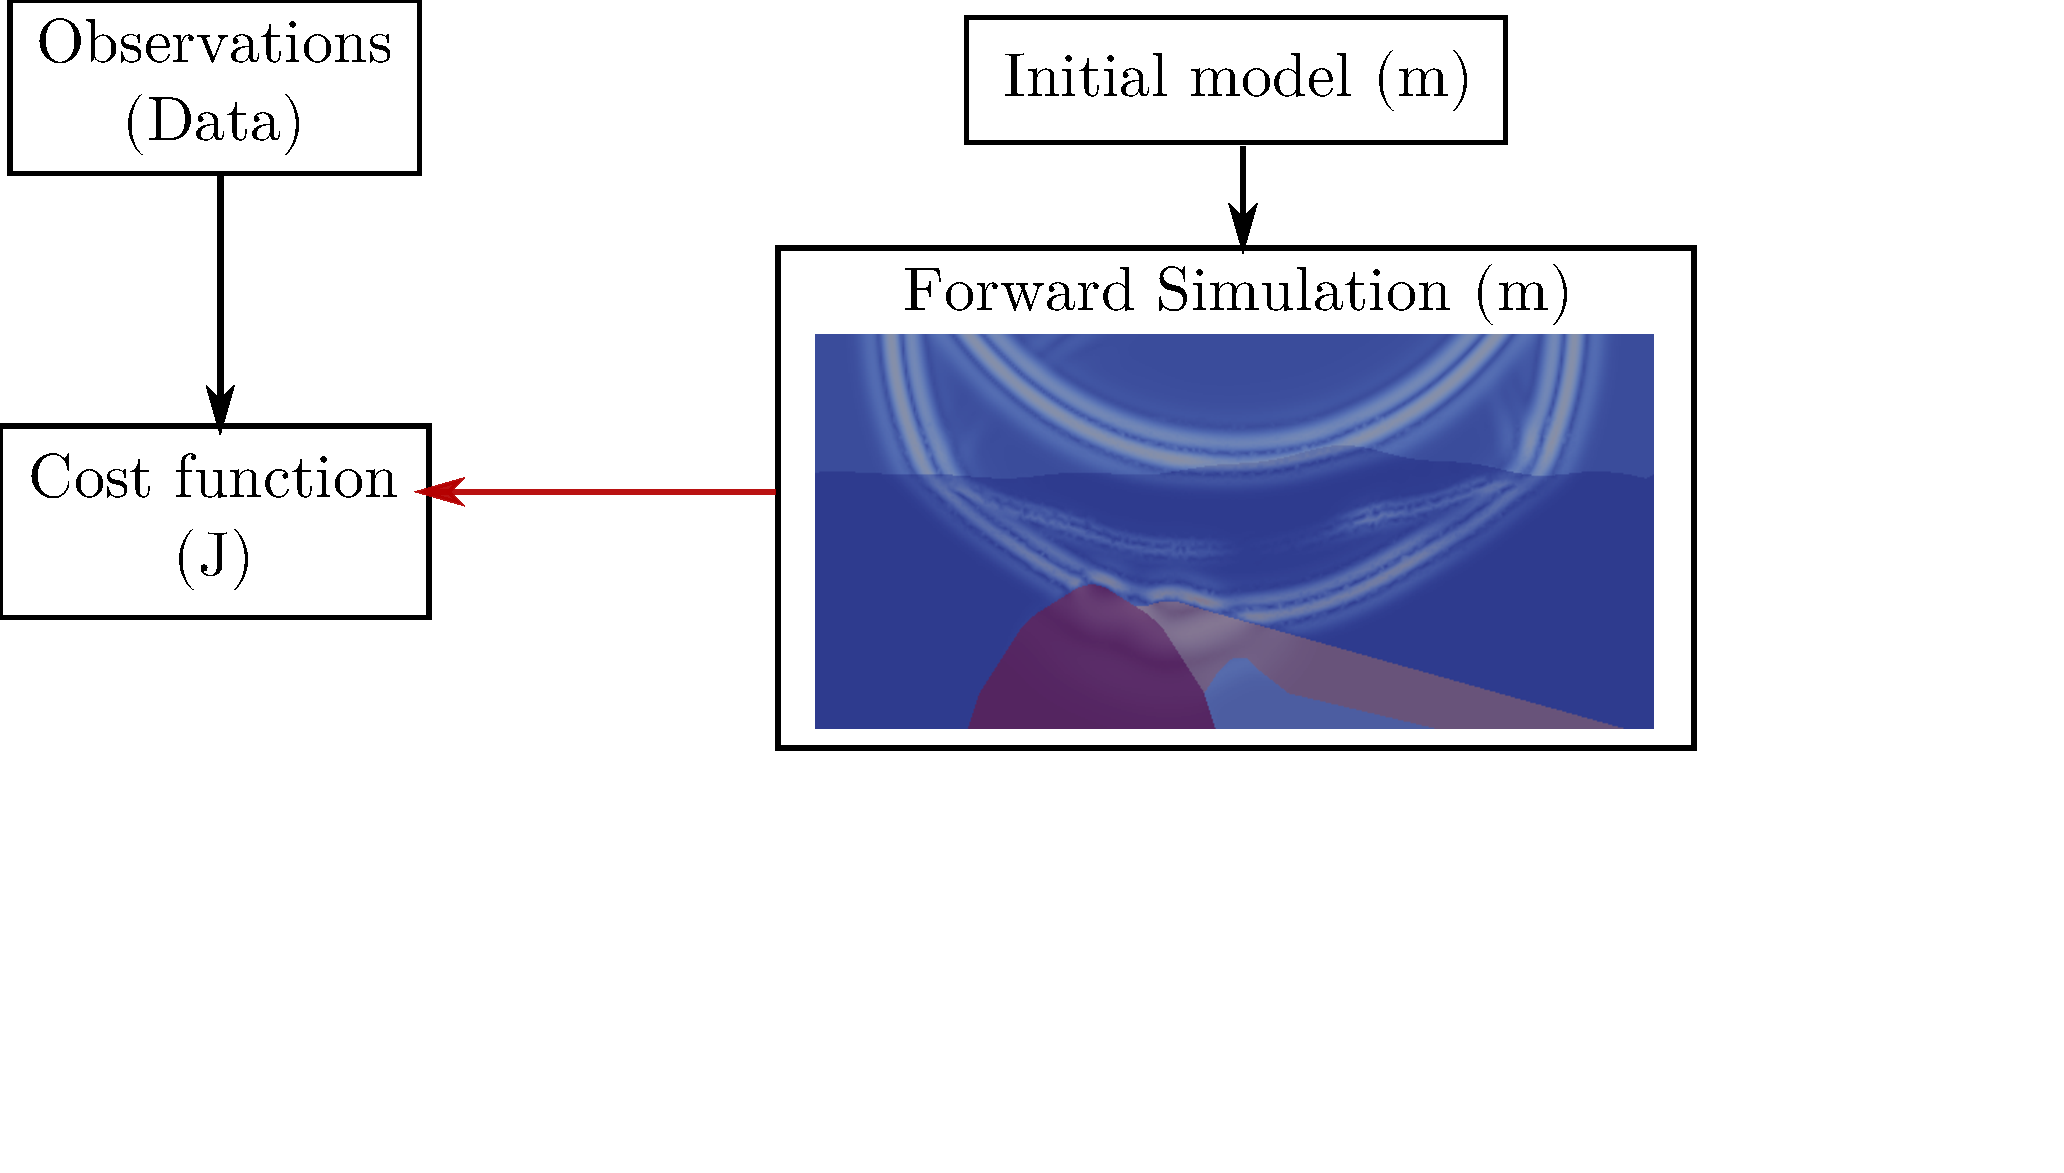
\includegraphics[scale=0.31]{fwi_test1.pdf}
\end{figure}
\end{frame}

\begin{frame}[noframenumbering]{FWI Workflow}
\begin{figure}
  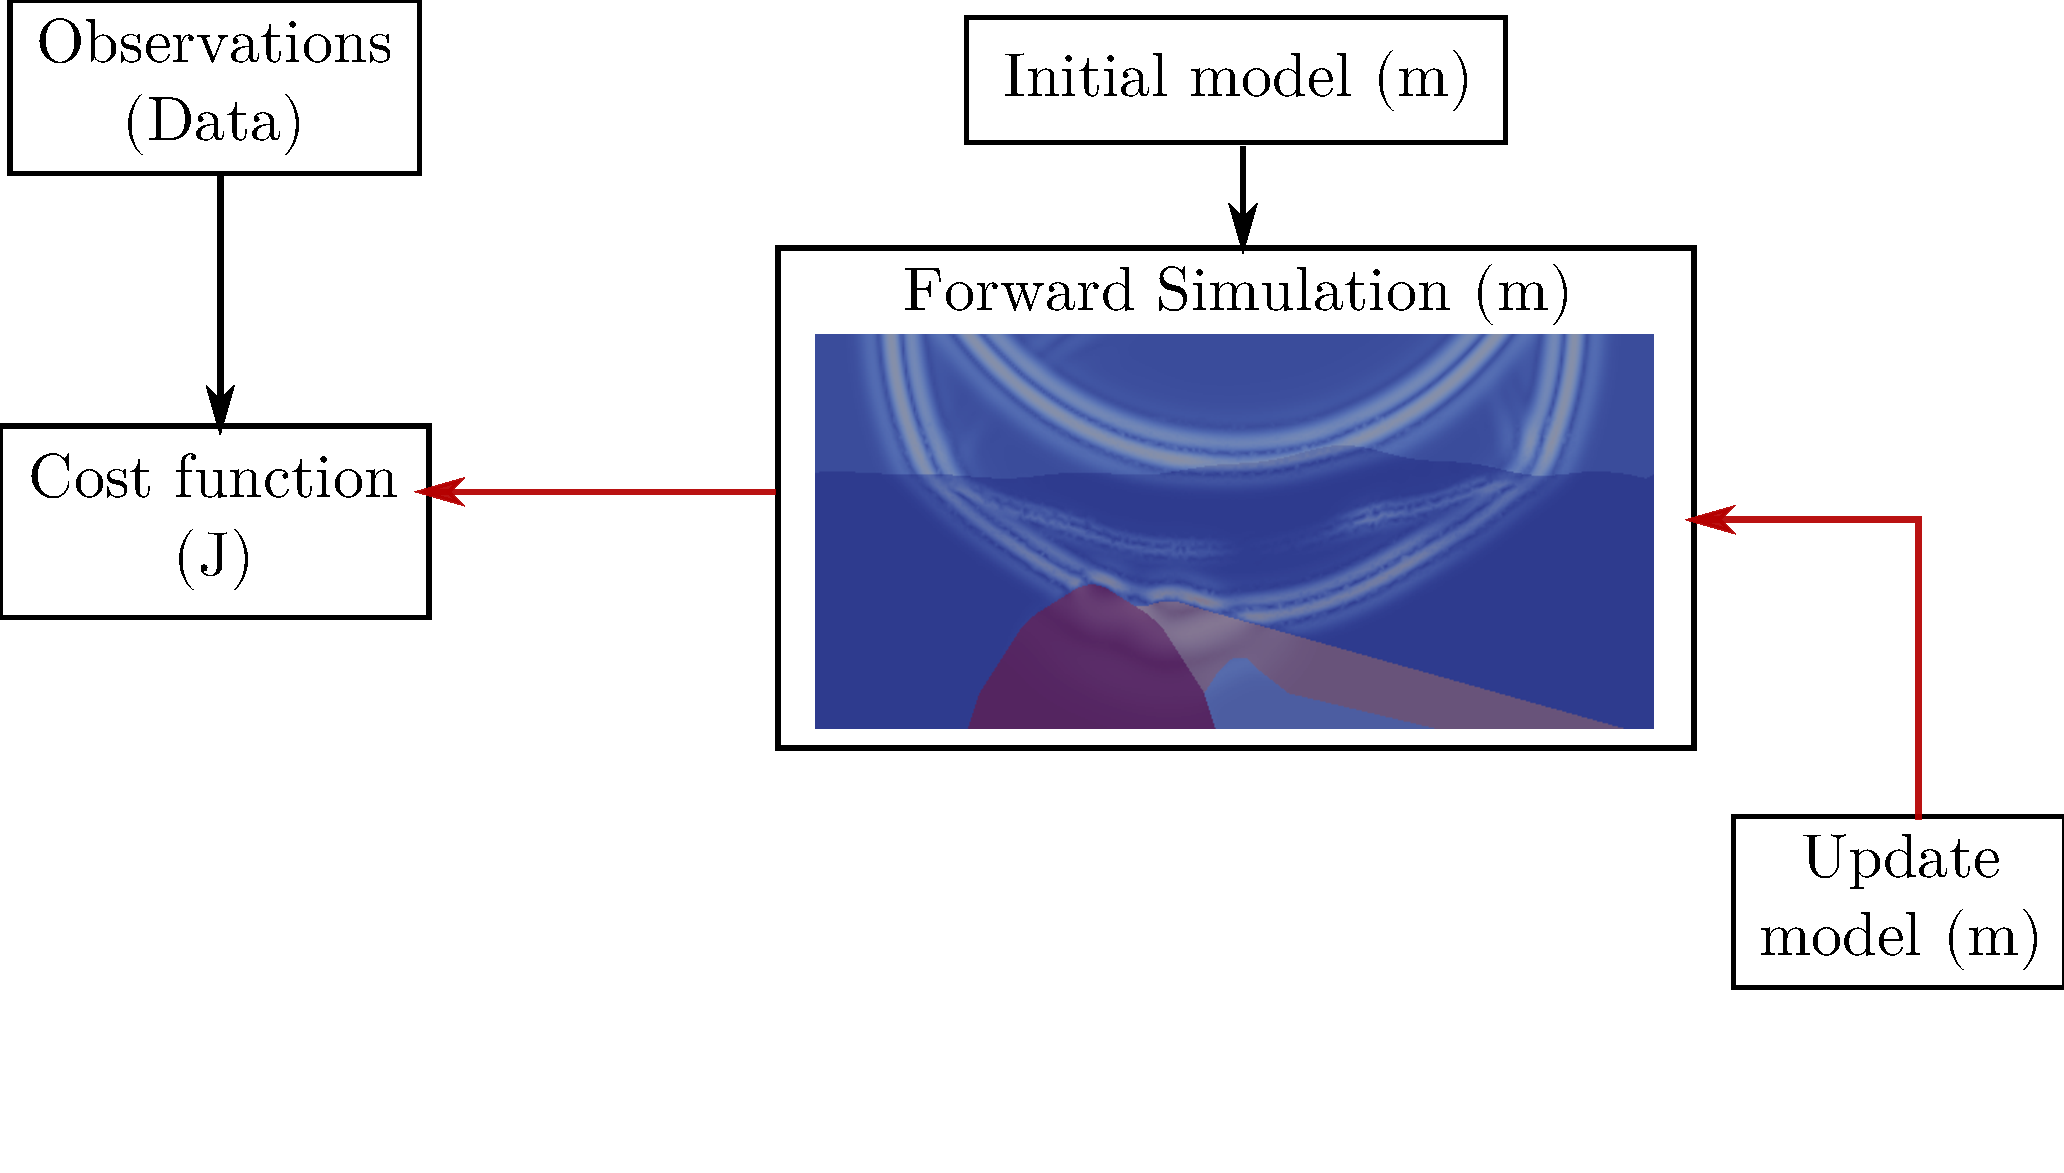
\includegraphics[scale=0.31]{fwi_test2.pdf}
\end{figure}
\end{frame}


\begin{frame}[noframenumbering]{FWI Workflow}
\begin{figure}
  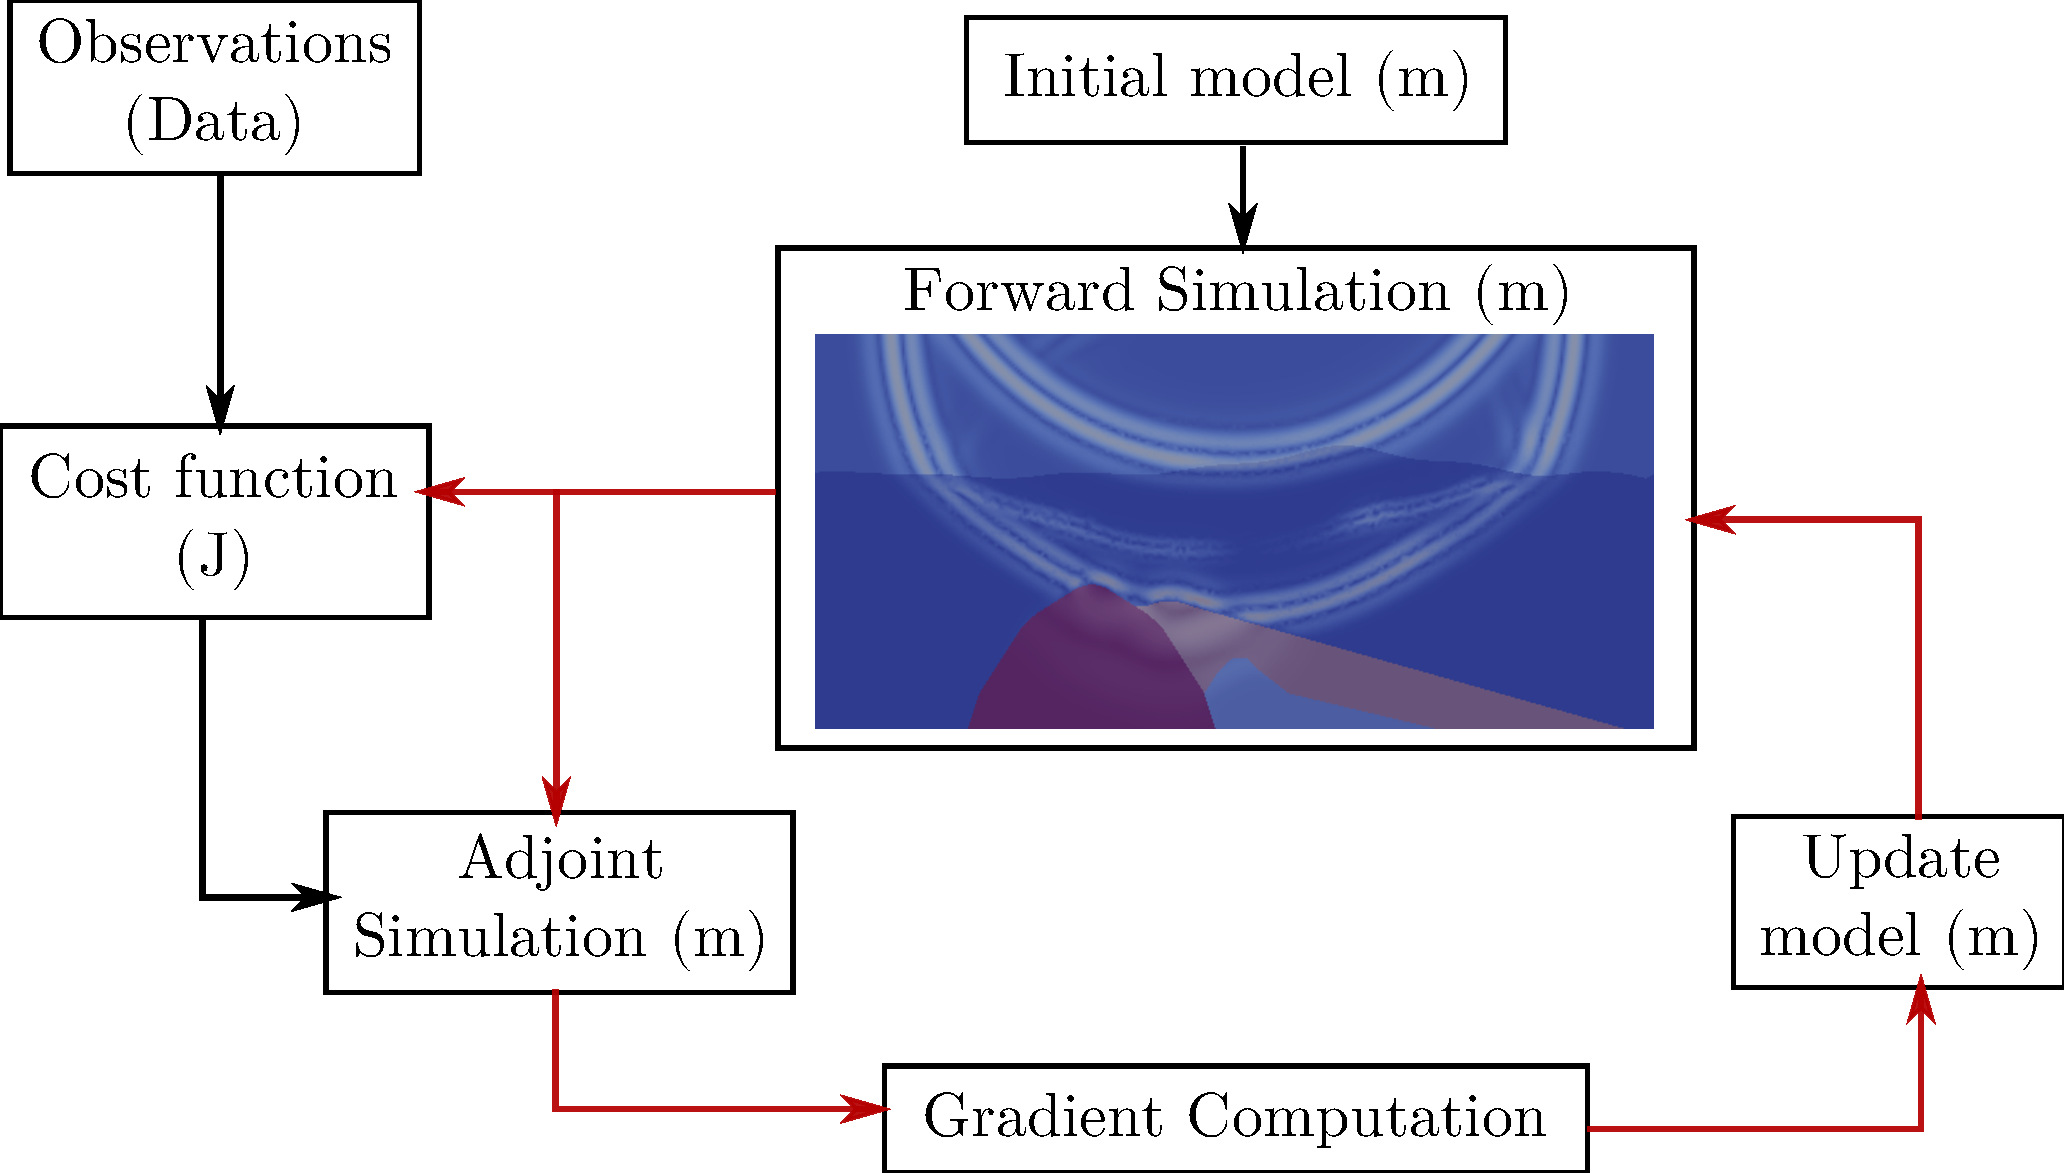
\includegraphics[scale=0.31]{fwi_test.pdf}
\end{figure}
\end{frame}

\begin{frame}[noframenumbering]{FWI Workflow}
\begin{figure}
  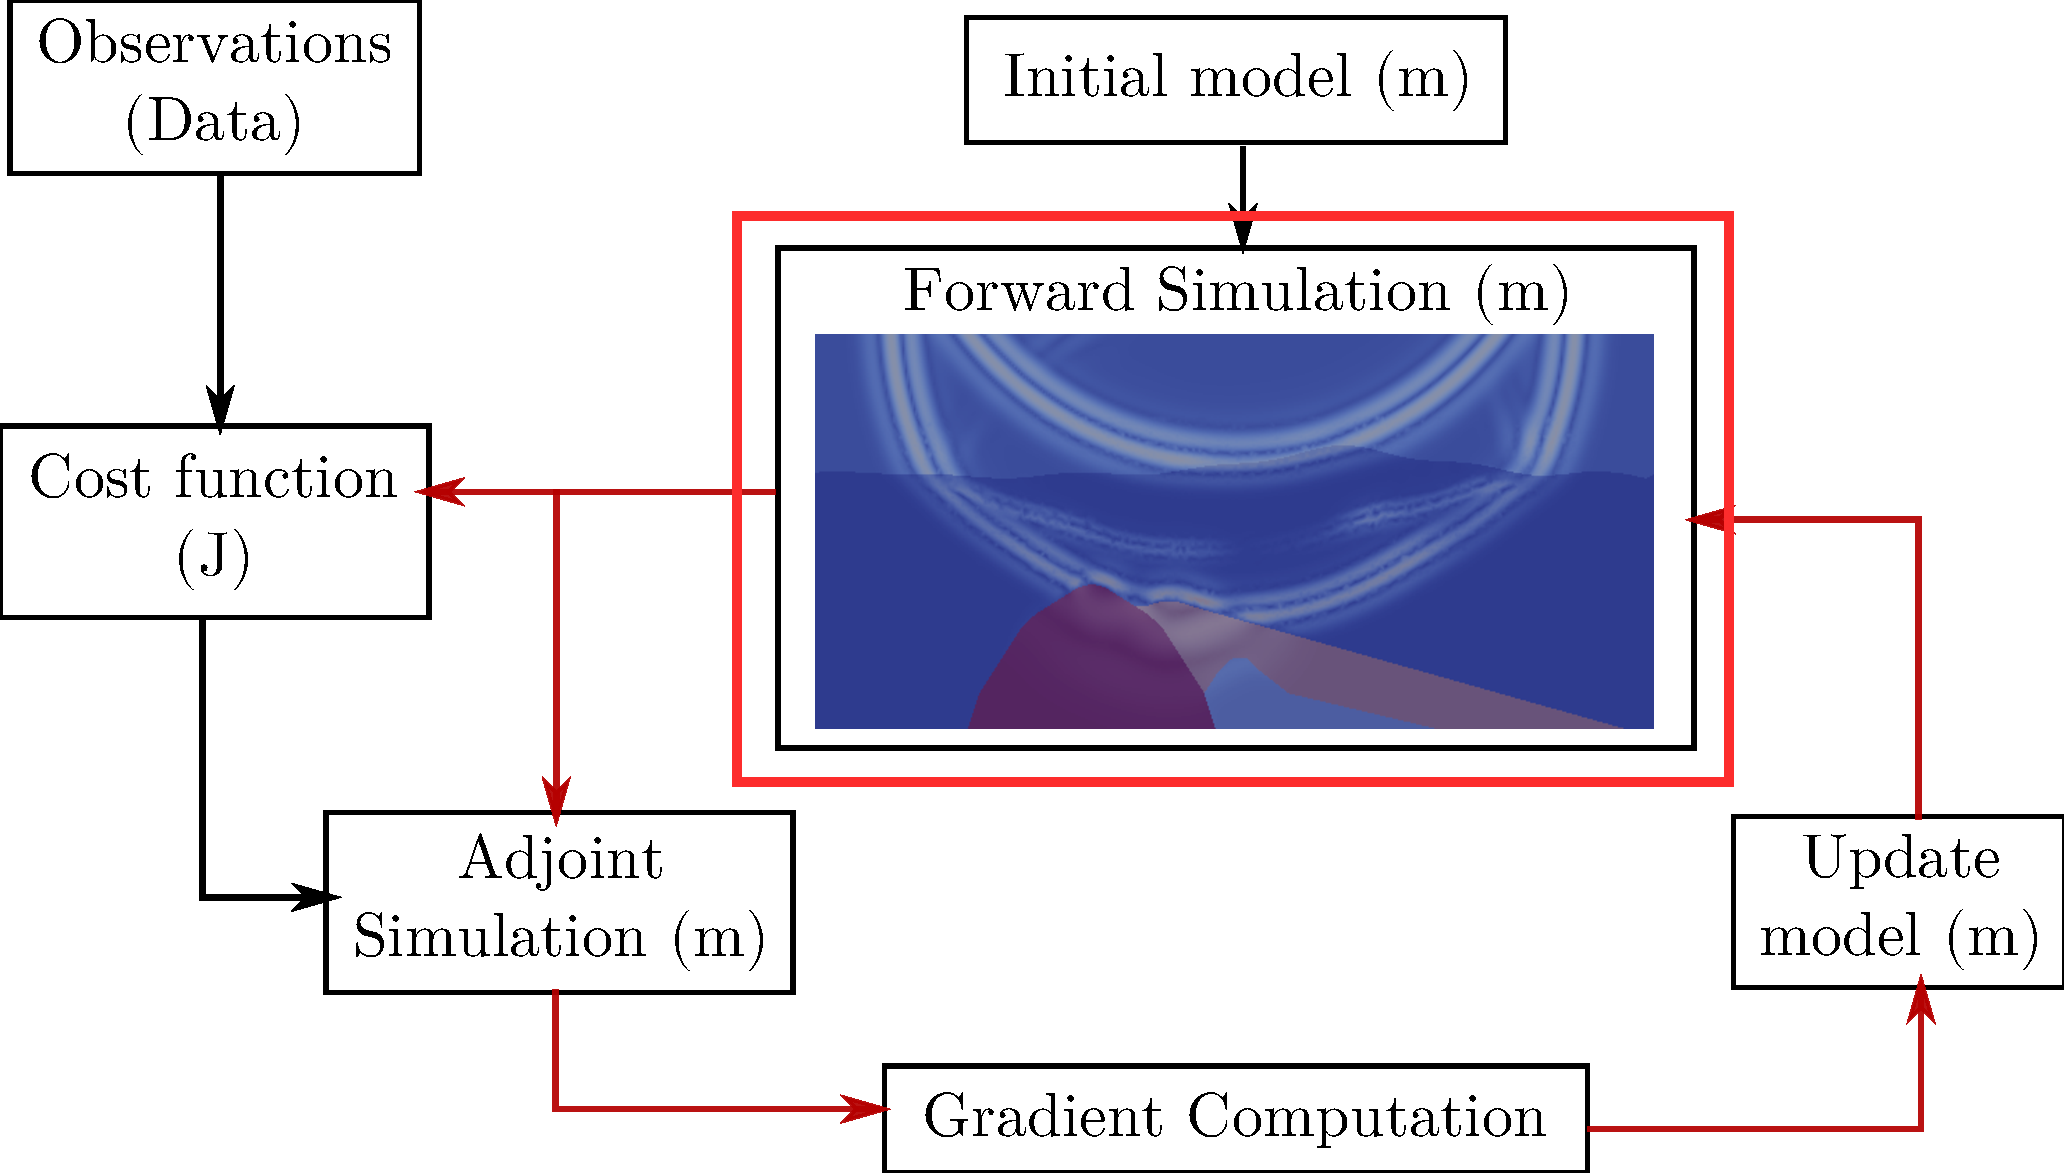
\includegraphics[scale=0.31]{fwi_test3.pdf}
\end{figure}
\end{frame}



% ============================================
% ====== Frame : Forward Continuous Model ====
% ============================================

\subsection{Forward Discretization}
\begin{frame}{Continuous Forward Model}

  First order acoustic wave equation
  \begin{multicols}{2}
  \begin{empheq}[left=\empheqlbrace]{align}
    & \frac{1}{\density \velocity^2}\frac{\partial \contP}{\partial t}+\nabla \cdot \contV=f_p \text{~~ on $\boldsymbol{\Omega}$}\\
    & \density\frac{\partial \contV}{\partial t}+\nabla\contP=0  \text{~~ on $\boldsymbol{\Omega}$}\\
    & \contP=0 \text{~~ on $\textcolor{red}{\boldsymbol{\Gamma_1}}$} \\
    & \frac{\partial \contP}{\partial t}+\velocity \nabla \contP \cdot \normal=0 \text{~~ on $\textcolor{blue}{\boldsymbol{\Gamma_2}}$}
  \end{empheq}

  \columnbreak

  \begin{center}
    \renewcommand\tikzscale{1.0}
    \begin{figure}[H]
    \begin{tikzpicture}[scale=\tikzscale]
\draw[color=blue,line width=2,double] (0,0) -- (5,0);
\draw[color=blue,line width=2,double] (0.07,-0.07) -- (0.07,3);
\draw[color=blue,line width=2,double] (4.93,-0.07) -- (4.93,3);
\draw[color=red,line width=2.1](-0.,3) -- (5,3);


\node[anchor=south, color=red]
at (2.5,3) {$\Gamma_1$};

\node[anchor=south, color=blue]
at (2.5,0) {$\Gamma_2$};

\node[color=black]
at (2.5,1.5) {$\Omega$};
\end{tikzpicture}

    \small{Domain with Absorbing Boundary Conditions}
    \end{figure}
  \end{center}

  \end{multicols}
\end{frame}





% ============================================
% ====== Frame : Forward Discrete Model ======
% ============================================

\begin{frame}{Discrete Forward Model}

  \begin{multicols}{2}

    Space Discretization : Discontinuous Galerkin Elements
    \begin{itemize}
      \item Nodal \small{(Lagrangian / Jacobian)}
      \item \normalsize{Modal} \small{(Bernstein-Bézier)}
    \end{itemize}
    \vspace{1cm}
    \uncover<3->{
    Time schemes :
    \begin{itemize}
      \item Runge Kutta 2/4
      \item Adams Bashforth 3
    \end{itemize}}

    \columnbreak

    \uncover<2->{
    Semi-discretized model :
    \begin{equation}
      \frac{\partial}{\partial t}\discreteU(t) = A \discreteU(t) + \discreteF(t)
    \end{equation}

    with :

    \begin{equation}
      \discreteU(t)=\vectll{(}{\discreteP(t)}{\discreteV(t)}{)}
    \end{equation}}

    \uncover<3->{
    \begin{figure}
      \noindent
       \begin{tikzpicture}[scale=0.8]
      \draw[color=black,line width=2.1](0.0,0.0) -- (5,0.0);
      %\draw[color=blue, line width=10] (0,-0.02) node {$\bullet$} ;
      %\draw[color=blue, line width=10] (5,-0.02) node {$\bullet$} ;
     % \draw node[color=blue,fill,circle,minimum size=0.01](1,1) {};
      \node[anchor=south east, color=black]
      at (0,0) {$0$};
      \node[anchor=south west, color=black]
      at (5,0) {$T$};
      
      \pgfmathsetmacro{\x}{0.0}
      \draw[color=black,line width=2.1](\x,0.1) -- (\x,-0.1);

      \pgfmathsetmacro{\x}{5.0}
      \draw[color=black,line width=2.1](\x,0.1) -- (\x,-0.1);

      \pgfmathsetmacro{\x}{0.5}
      \draw[color=black,line width=1.5](\x,0.1) -- (\x,-0.1);
      \draw[arrowStyle,color=blue]
      (\x-0.5,0) to[out=90,in=90,looseness=4.0]
      node[sloped,anchor=south]
      {}
      (\x,0.0);
      \draw[color=black,line width=1.5](\x,0.1) -- (\x,-0.1);


      
      \pgfmathsetmacro{\x}{1.0}
            \draw[arrowStyle,color=blue]
      (\x-0.5,0) to[out=90,in=90,looseness=4.0]
      node[sloped,anchor=south]
      {}
      (\x,0.0);
      \draw[color=black,line width=1.5](\x,0.1) -- (\x,-0.1);
      \pgfmathsetmacro{\x}{1.5}
            \draw[arrowStyle,color=blue]
      (\x-0.5,0) to[out=90,in=180,looseness=1.0]
      node[sloped,anchor=south]
      {}
      (\x,0.55);

      
      \draw[color=black,line width=1.5](\x,0.1) -- (\x,-0.1);
      \pgfmathsetmacro{\x}{2.0}
      \draw[color=black,line width=1.5](\x,0.1) -- (\x,-0.1);
      \pgfmathsetmacro{\x}{2.5}
      \draw[color=black,line width=1.5](\x,0.1) -- (\x,-0.1);
      \pgfmathsetmacro{\x}{3.0}
      \draw[color=black,line width=1.5](\x,0.1) -- (\x,-0.1);
      \pgfmathsetmacro{\x}{3.5}
      \draw[color=black,line width=1.5](\x,0.1) -- (\x,-0.1);
      \pgfmathsetmacro{\x}{4.0}
      \draw[color=black,line width=1.5](\x,0.1) -- (\x,-0.1);
      \pgfmathsetmacro{\x}{4.5}
      \draw[color=black,line width=1.5](\x,0.1) -- (\x,-0.1);
    \end{tikzpicture}

      Forward time steps
    \end{figure}}

  \end{multicols}

\end{frame}






% ============================================
% ====== Frame : Asset of DGs  ===============
% ============================================

\begin{frame}{Discrete Forward Model}{Discontinuous Galerkin Method}
  Asset of Discontinuous Galerkin Methods : \\

  \begin{itemize}
  \item Unstructured grid (enable to match the topography and media irregularities)
  \item Robust to physical discontinuities
  \item hp-adaptivity
  \item Massively parallel performance properties
  \end{itemize}

  \begin{figure}[H]
    \centering
    \subfigure[h-adaptivity]{
      \begin{tikzpicture}[scale=0.7]%[line cap=round,line join=round,>=triangle 45,x=1.0cm,y=1.0cm]
      %% \draw[->,color=black] (-1.05,0) -- (9.66,0);
      %% \foreach \x in {-1,-0.5,0.5,1,1.5,2,2.5,3,3.5,4,4.5,5,5.5,6,6.5,7,7.5,8,8.5,9,9.5}
      %% \draw[shift={(\x,0)},color=black] (0pt,2pt) -- (0pt,-2pt) node[below] {\footnotesize $\x$};
      %% \draw[->,color=black] (0,-0.43) -- (0,5.53);
      %% \foreach \y in {,0.5,1,1.5,2,2.5,3,3.5,4,4.5,5,5.5}
      %% \draw[shift={(0,\y)},color=black] (2pt,0pt) -- (-2pt,0pt) node[left] {\footnotesize $\y$};
      %% \draw[color=black] (0pt,-10pt) node[right] {\footnotesize $0$};
      %% \clip(-1.05,-0.43) rectangle (9.66,5.53);
      \fill[line width=2.4pt,fill=black,fill opacity=0.1] (1,1) -- (4,2) -- (4,1) -- cycle;
      \fill[line width=2.4pt,fill=black,fill opacity=0.1] (1,1) -- (1,4) -- (2,4) -- cycle;
      \fill[line width=2.4pt,fill=black,fill opacity=0.1] (2,4) -- (4,2) -- (1,1) -- cycle;
      \fill[line width=2.4pt,fill=black,fill opacity=0.1] (2,4) -- (4,4) -- (4,2) -- cycle;
      \draw [line width=2.4pt] (1,1)-- (4,2);
      \draw [line width=2.4pt] (4,2)-- (4,1);
      \draw [line width=2.4pt] (4,1)-- (1,1);
      \draw [line width=2.4pt] (1,1)-- (1,4);
      \draw [line width=2.4pt] (1,4)-- (2,4);
      \draw [line width=2.4pt] (2,4)-- (1,1);
      \draw [line width=2.4pt] (2,4)-- (4,2);
      \draw [line width=2.4pt] (4,2)-- (1,1);
      \draw [line width=2.4pt] (1,1)-- (2,4);
      \draw [line width=2.4pt] (2,4)-- (4,4);
      \draw [line width=2.4pt] (4,4)-- (4,2);
      \draw [line width=2.4pt] (4,2)-- (2,4);
      \draw [line width=2.4pt] (2,4)-- (3.5,3.5);
      \draw [line width=2.4pt] (3,3)-- (4,4);
      \draw [line width=2.4pt] (4,4)-- (2,4);
      \draw [line width=2.4pt] (2,4)-- (3.5,3.5);
      \draw [line width=2.4pt] (3.5,3.5)-- (4,2);
      \draw [line width=2.4pt] (4,2)-- (2,4);
      \draw [line width=2.4pt] (4,2)-- (4,4);
      \draw [line width=2.4pt] (4,4)-- (3.5,3.5);
      \draw [line width=2.4pt] (3.5,3.5)-- (4,2);
  \end{tikzpicture}

}
    \hspace{1cm}
  \subfigure[p-adaptivity with \textcolor{black}{P1}, \textcolor{blue}{P2}, \textcolor{red}{P3} elements]{
      \definecolor{ccqqqq}{rgb}{0.8,0,0}
    \definecolor{qqqqff}{rgb}{0,0,1}
    \definecolor{cccccc}{rgb}{0.8,0.8,0.8}
    \begin{tikzpicture}[scale=0.7]
      %\draw[->,color=black] (0,0.62) -- (0,4.91);
      %\foreach \y in {0.6,0.8,1,1.2,1.4,1.6,1.8,2,2.2,2.4,2.6,2.8,3,3.2,3.4,3.6,3.8,4,4.2,4.4,4.6,4.8}
      %\draw[shift={(0,\y)},color=black] (2pt,0pt) -- (-2pt,0pt) node[left] {\footnotesize $\y$};
      %\clip(-0.64,0.62) rectangle (7.09,4.91);
      \fill[line width=1.6pt,color=cccccc,fill=cccccc,fill opacity=0.15] (1,1) -- (1,4) -- (4,4) -- (4,1) -- cycle;
      \fill[fill=black,fill opacity=0.1] (1,1) -- (2.5,2.5) -- (4,1) -- cycle;
      \fill[fill=black,fill opacity=0.1] (1,1) -- (2.5,2.5) -- (1,4) -- cycle;
      \fill[fill=black,fill opacity=0.1] (1,4) -- (4,4) -- (2.5,2.5) -- cycle;
      \fill[fill=black,fill opacity=0.1] (4,1) -- (2.5,2.5) -- (4,4) -- cycle;
      \draw [line width=2.8pt] (1,1)-- (1,4);
      \draw [line width=2.8pt] (1,4)-- (4,4);
      \draw [line width=2.8pt] (4,4)-- (4,1);
      \draw [line width=2.8pt] (4,1)-- (1,1);
      \draw [line width=2.8pt] (1,1)-- (2.5,2.5);
      \draw [line width=2.8pt] (2.5,2.5)-- (4,1);
      \draw [line width=2.8pt] (4,1)-- (1,1);
      \draw [line width=2.8pt] (1,1)-- (2.5,2.5);
      \draw [line width=2.8pt] (2.5,2.5)-- (1,4);
      \draw [line width=2.8pt] (1,4)-- (1,1);
      \draw [line width=2.8pt] (1,4)-- (4,4);
      \draw [line width=2.8pt] (4,4)-- (2.5,2.5);
      \draw [line width=2.8pt] (2.5,2.5)-- (1,4);
      \draw [line width=2.8pt] (4,1)-- (2.5,2.5);
      \draw [line width=2.8pt] (2.5,2.5)-- (4,4);
      \draw [line width=2.8pt] (4,4)-- (4,1);
      \begin{scriptsize}
        \fill [color=black] (1.07,3.76) circle (2.321pt);
        \fill [color=black] (1.08,1.24) circle (2.321pt);
        \fill [color=black] (2.3,2.5) circle (2.321pt);
        \fill [color=qqqqff] (2.51,2.3) circle (2.321pt);
        \fill [color=qqqqff] (2.72,2.5) circle (2.321pt);
        \fill [color=ccqqqq] (2.5,2.71) circle (2.321pt);
        \fill [color=qqqqff] (3.77,1.09) circle (2.321pt);
        \fill [color=qqqqff] (3.91,1.22) circle (2.321pt);
        \fill [color=ccqqqq] (3.73,3.87) circle (2.321pt);
        \fill [color=qqqqff] (3.89,3.75) circle (2.321pt);
        \fill [color=qqqqff] (1.24,1.11) circle (2.321pt);
        \fill [color=qqqqff] (1.87,1.7) circle (2.321pt);
        \fill [color=qqqqff] (3.14,1.69) circle (2.321pt);
        \fill [color=qqqqff] (2.51,1.1) circle (2.321pt);
        \fill [color=qqqqff] (3.31,1.86) circle (2.321pt);
        \fill [color=qqqqff] (3.9,2.48) circle (2.321pt);
        \fill [color=qqqqff] (3.31,3.13) circle (2.321pt);
        \fill [color=ccqqqq] (1.23,3.9) circle (2.321pt);
        \fill [color=ccqqqq] (2.08,3.87) circle (2.321pt);
        \fill [color=ccqqqq] (2.97,3.86) circle (2.321pt);
        \fill [color=ccqqqq] (1.63,3.56) circle (2.321pt);
        \fill [color=ccqqqq] (2.15,3.06) circle (2.321pt);
        \fill [color=ccqqqq] (3.36,3.54) circle (2.321pt);
        \fill [color=ccqqqq] (2.83,3.05) circle (2.321pt);
        \fill [color=ccqqqq] (2.49,3.55) circle (2.321pt);
      \end{scriptsize}
  \end{tikzpicture}

  }
\end{figure}
\end{frame}
  %% intro FWI
%% \section{Adjoint Studies}
\renewcommand\tikzscale{1.3}


% ============================================
% ====== Frame : Adjoint State Method  =======
% ============================================

\begin{frame}{Adjoint State Method}

Lagrangian fonctional :
  \begin{equation}
    \Lag(\qcqU,\qcqLbd,\model) = \frac{1}{2}||\textcolor{blue}{d_{obs}}-\textcolor{red}{\mathcal{R}(\qcqU)}||^2dt + <\DP(\qcqU),\qcqLbd>
  \end{equation}

    If $\qcqU=\contU$ Solution of the Direct Problem $\Longleftrightarrow$ ($\DP(\contU) = 0$) :

  \begin{equation}
    \CF(\model) = \Lag(\contU,\qcqLbd,\model)
  \end{equation}

  \uncover<2->{
  Let us choose $\qcqLbd=\contLbd$ such as $\frac{\partial \Lag}{\partial \contU} = 0$

  \begin{equation}
    (\mathcal{R}^*\textcolor{blue}{d_{obs}}-\contU) + \DP^*(\contLbd) = 0
  \end{equation}
  }

  \uncover<3->{
  For $\DP(\contU) = 0$ :

  \begin{equation}
    \partial_{\model_i} \CF(\model) = \partial_{\model_i} \Lag(\contU,\contLbd,\model) = \partial_{\model_i} <\DP(\contU),\contLbd>
  \end{equation}
}

\end{frame}











% ============================================
% ====== Frame : Adjoint Scheme      =========
% ============================================
\begin{frame}{Adjoint Formulation}
\begin{figure}

\definecolor{color1}{RGB}{255,174,41}   %% myOrange
%\definecolor{color2}{RGB}{216,93,99}  %% myGreen
\definecolor{color3}{RGB}{100,149,237} %% myBlue
\definecolor{color2}{RGB}{223,83,74} %% myRed

\definecolor{colorOne}{RGB}{255,174,41}   %% myOrange
%\definecolor{color2}{RGB}{216,93,99}  %% myGreen
\definecolor{colorThree}{RGB}{100,149,237} %% myBlue
\definecolor{colorTwo}{RGB}{223,83,74} %% myRed


\begin{tikzpicture}[scale=\tikzscale] %% [every node/.style={scale=1}]

\node[boxOptions]
at (0,3.5){ {\textbf{\Large\fontfamily{pzc}\selectfont Continuous \\ Direct Problem}}};

\uncover<2->{
\node[boxOptions]
at (6,3.5){ {\textbf{\Large\fontfamily{pzc}\selectfont Continuous \\ Adjoint Problem}}};

\coordinate (a) at (1.4,3.5);
\coordinate (b) at (4.7,3.5);
\draw[->, >=latex, red!50!white, line width=10pt]   (a) to node[pos=0.4,above]{\small{\textbf{\textcolor{black}{Adjoint}}}} (b) ;
}

\uncover<3->{
\node[boxOptions]
at (6,0.7){\textbf{Discretization of the Continuous Adjoint Problem}};

\draw[arrowStyleinv]
(6,2.1) to[out=90,in=90]
node[sloped,anchor=south]
{}
(6,2.6);

\coordinate (b) at (6,1.2);
\coordinate (a) at (6,3.0);
\draw[->, >=latex, red!50!white, line width=10pt]   (a) to node[fill=colorThree!0,pos=0.3]{\small{\textbf{\textcolor{black}{Discretization}}}} (b) ;
}


\uncover<4->{
\node[boxOptions]
at (0,-0.5){\textbf{Discrete \\Direct Problem}};

%% \draw[arrowStyleinv]
%% (0,0.7) to[out=90,in=90]
%% node[sloped,anchor=south]
%% {\footnotesize{Discretization ~~~~~~~~~~~~~}}
%% (0,2.5);

\coordinate (b) at (0,-0.1);
\coordinate (a) at (0,3.0);
\draw[->, >=latex, blue!50!white, line width=10pt]   (a) to node[fill=colorThree!0]{\small{\textbf{\textcolor{black}{Discretization}}}} (b) ;


\node[boxOptions]
at (6,-0.5){\textbf{Adjoint of the Discrete Problem}};


%% \draw[arrowStyle]
%% (2,0) to[out=0,in=180]
%% node[sloped,anchor=south]
%% {(*)}
%% (4,0);

\coordinate (a) at (1.4,-0.5);
\coordinate (b) at (4.7,-0.5);
\draw[->, >=latex, blue!50!white, line width=10pt]   (a) to node[pos=0.4,below]{\small{\textbf{\textcolor{black}{Adjoint}}}} (b) ;
}

\uncover<5->{
\draw[color=red,line width=2] (4.5,1.4)
rectangle (7.5,-1.0);
}
\end{tikzpicture}
\end{figure}
\end{frame}








% ============================================
% ====== Frame : Adjoint then discretize 1 ===
% ============================================

\begin{frame}{AtD : Adjoint then Discretized Strategy}

  \begin{equation}
    \CF(\contP)=\frac{1}{2}||\textcolor{blue}{d_{obs}} - R\contP||^2
    \end{equation}

  \noindent
  \begin{multicols}{2}
    \noindent
      \begin{empheq}[left=\empheqlbrace]{align}
    & \frac{1}{\density \velocity^2}\frac{\partial \contP}{\partial t}+\nabla \cdot \contV=f_p \text{~~ on $\boldsymbol{\Omega}$}\\
    & \density\frac{\partial \contV}{\partial t}+\nabla\contP=0  \text{~~ on $\boldsymbol{\Omega}$}\\
    & \contP=0 \text{~~ on $\textcolor{red}{\boldsymbol{\Gamma_1}}$} \\
    & \frac{\partial \contP}{\partial t}+\velocity \nabla \contP \cdot \normal=0 \text{~~ on $\textcolor{blue}{\boldsymbol{\Gamma_2}}$}\\
    & \contP(0) = 0 \text{, ~~~} \contV(0) = 0
      \end{empheq}
      \vspace{30cm}
    \columnbreak
    \noindent
      \begin{empheq}[left=\empheqlbrace]{align}
    & \frac{1}{\density \velocity^2}\frac{\partial \Lbdun}{\partial t}+\nabla \cdot \Lbdeux=\frac{\partial \CF}{\partial \contP} \text{~~ on $\boldsymbol{\Omega}$}\\
    & \density\frac{\partial \Lbdeux}{\partial t}+\nabla\Lbdun=0  \text{~~ on $\boldsymbol{\Omega}$}\\
    & \Lbdun=0 \text{~~ on $\textcolor{red}{\boldsymbol{\Gamma_1}}$} \\
    & \frac{\partial \Lbdun}{\partial t}-\velocity \nabla \Lbdun \cdot \normal=0 \text{~~ on $\textcolor{blue}{\boldsymbol{\Gamma_2}}$}\\
    & \Lbdun(T) = 0 \text{, ~~~} \Lbdeux(T) = 0
  \end{empheq}

  \end{multicols}
  \vspace{-0.5cm}
  \begin{equation}
    t\in[0,T] \text{~~~~~~~~~~~~~~~~~~~~~~~~~~} t\in[T,0]
    \end{equation}
\end{frame}





% ============================================
% ====== Frame : Adjoint then discretize 2 ===
% ============================================

\subsection{Adjoint then Discretized}
\begin{frame}{AtD : Adjoint then Discretized Strategy}

  \begin{equation}
    \CF(\contP)=\frac{1}{2}||\textcolor{blue}{d_{obs}} - R\contP||^2
  \end{equation}

  \noindent
  \begin{multicols}{2}
    \noindent
    \begin{empheq}[left=\empheqlbrace]{align}
  & \frac{\partial \discreteU}{\partial t}^n=A\discreteU^n+ \discreteF^n \\[0.2cm]
  & \text{With : ~~}  \discreteU^n=\vectll{(}{\discreteP^n}{\discreteV^n}{)}
    \end{empheq}
    \vspace{0.3cm}
    \begin{figure}
      \noindent
       \begin{tikzpicture}[scale=0.8]
      \draw[color=black,line width=2.1](0.0,0.0) -- (5,0.0);
      %\draw[color=blue, line width=10] (0,-0.02) node {$\bullet$} ;
      %\draw[color=blue, line width=10] (5,-0.02) node {$\bullet$} ;
     % \draw node[color=blue,fill,circle,minimum size=0.01](1,1) {};
      \node[anchor=south east, color=black]
      at (0,0) {$0$};
      \node[anchor=south west, color=black]
      at (5,0) {$T$};
      
      \pgfmathsetmacro{\x}{0.0}
      \draw[color=black,line width=2.1](\x,0.1) -- (\x,-0.1);

      \pgfmathsetmacro{\x}{5.0}
      \draw[color=black,line width=2.1](\x,0.1) -- (\x,-0.1);

      \pgfmathsetmacro{\x}{0.5}
      \draw[color=black,line width=1.5](\x,0.1) -- (\x,-0.1);
      \draw[arrowStyle,color=blue]
      (\x-0.5,0) to[out=90,in=90,looseness=4.0]
      node[sloped,anchor=south]
      {}
      (\x,0.0);
      \draw[color=black,line width=1.5](\x,0.1) -- (\x,-0.1);


      
      \pgfmathsetmacro{\x}{1.0}
            \draw[arrowStyle,color=blue]
      (\x-0.5,0) to[out=90,in=90,looseness=4.0]
      node[sloped,anchor=south]
      {}
      (\x,0.0);
      \draw[color=black,line width=1.5](\x,0.1) -- (\x,-0.1);
      \pgfmathsetmacro{\x}{1.5}
            \draw[arrowStyle,color=blue]
      (\x-0.5,0) to[out=90,in=180,looseness=1.0]
      node[sloped,anchor=south]
      {}
      (\x,0.55);

      
      \draw[color=black,line width=1.5](\x,0.1) -- (\x,-0.1);
      \pgfmathsetmacro{\x}{2.0}
      \draw[color=black,line width=1.5](\x,0.1) -- (\x,-0.1);
      \pgfmathsetmacro{\x}{2.5}
      \draw[color=black,line width=1.5](\x,0.1) -- (\x,-0.1);
      \pgfmathsetmacro{\x}{3.0}
      \draw[color=black,line width=1.5](\x,0.1) -- (\x,-0.1);
      \pgfmathsetmacro{\x}{3.5}
      \draw[color=black,line width=1.5](\x,0.1) -- (\x,-0.1);
      \pgfmathsetmacro{\x}{4.0}
      \draw[color=black,line width=1.5](\x,0.1) -- (\x,-0.1);
      \pgfmathsetmacro{\x}{4.5}
      \draw[color=black,line width=1.5](\x,0.1) -- (\x,-0.1);
    \end{tikzpicture}

Time-steps going Forward
    \end{figure}
    \columnbreak
    \noindent
    \begin{empheq}[left=\empheqlbrace]{align}
   \boldsymbol{~~~}   & \frac{\partial \discreteLbd}{\partial t}^n=A\discreteLbd^n+R^*(R\discreteU^n-\textcolor{blue}{d_{obs}})\\
  & \text{With : ~~}  \discreteLbd^n=\vectll{(}{\discreteLbdun^n}{\discreteLbdeux^n}{)}
    \end{empheq}
    \vspace{-0.0cm}
    \noindent
    \begin{figure}
      \noindent
       \begin{tikzpicture}[scale=0.8]
      \draw[color=black,line width=2.1](0.0,0.0) -- (5,0.0);
      %\draw[color=blue, line width=10] (0,-0.02) node {$\bullet$} ;
      %\draw[color=blue, line width=10] (5,-0.02) node {$\bullet$} ;
     % \draw node[color=blue,fill,circle,minimum size=0.01](1,1) {};
      \node[anchor=south east, color=black]
      at (0,0) {$0$};
      \node[anchor=south west, color=black]
      at (5,0) {$T$};
      
      \pgfmathsetmacro{\x}{0.0}
      \draw[color=black,line width=2.1](\x,0.1) -- (\x,-0.1);

      \pgfmathsetmacro{\x}{5.0}
      \draw[color=black,line width=2.1](\x,0.1) -- (\x,-0.1);

      \pgfmathsetmacro{\x}{0.5}
      \draw[color=black,line width=1.5](\x,0.1) -- (\x,-0.1);
      \draw[color=black,line width=1.5](\x,0.1) -- (\x,-0.1);


      
      \pgfmathsetmacro{\x}{1.0}
      \draw[color=black,line width=1.5](\x,0.1) -- (\x,-0.1);
      \pgfmathsetmacro{\x}{1.5}
      \draw[color=black,line width=1.5](\x,0.1) -- (\x,-0.1);
      \pgfmathsetmacro{\x}{2.0}
      \draw[color=black,line width=1.5](\x,0.1) -- (\x,-0.1);
      \pgfmathsetmacro{\x}{2.5}
      \draw[color=black,line width=1.5](\x,0.1) -- (\x,-0.1);
      \pgfmathsetmacro{\x}{3.0}
      \draw[color=black,line width=1.5](\x,0.1) -- (\x,-0.1);
      \pgfmathsetmacro{\x}{3.5}


      \draw[arrowStyle,color=blue]
      (\x+0.5,0) to[out=90,in=0,looseness=1.0]
      node[sloped,anchor=south]
      {}
      (\x,0.55);
      

      
      \draw[color=black,line width=1.5](\x,0.1) -- (\x,-0.1);
      \pgfmathsetmacro{\x}{4.0}


      \draw[arrowStyle,color=blue]
      (\x+0.5,0) to[out=90,in=90,looseness=4.0]
      node[sloped,anchor=south]
      {}
      (\x,0.0);
      
      
      \draw[color=black,line width=1.5](\x,0.1) -- (\x,-0.1);
      \pgfmathsetmacro{\x}{4.5}

      \draw[arrowStyle,color=blue]
      (\x+0.5,0) to[out=90,in=90,looseness=4.0]
      node[sloped,anchor=south]
      {}
      (\x,0.0);
      
      \draw[color=black,line width=1.5](\x,0.1) -- (\x,-0.1);
    \end{tikzpicture}

      Time-steps going Backward
    \end{figure}
  \end{multicols}
\end{frame}







\subsection{Discretize then Adjoint}

% ============================================
% ====== Frame : Discretize then Adjoint 1 ===
% ============================================
\begin{frame}{DtA : Discretize then Adjoint Strategy}{Example With RK4}

  All time scheme can be summed-up such as :
  \begin{equation}
    \textcolor{\myblue}{\boldsymbol{L}}\discreteU=\textcolor{\myblue}{\boldsymbol{E}}\discreteF
  \end{equation}

  \small
      RK4 time-scheme leads to :
    \begin{equation}
      \discreteU^{n+1}=B\discreteU^n+\textcolor{\myblue}{\boldsymbol{C_0}}\discreteF^n+\textcolor{\myblue}{\boldsymbol{C_{\frac{1}{2}}}}\discreteF^{n+\frac{1}{2}}+\textcolor{\myblue}{\boldsymbol{C_1}}\discreteF^{n+1}
    \end{equation}

\begin{equation}
  \textcolor{\myblue}{\boldsymbol{L}}\discreteU=\textcolor{\myblue}{\boldsymbol{E}}\discreteF=\discreteG
\end{equation}
\begin{equation}
  \begin{pmatrix}
    I & & & & \\
    -B&I & & & \\
    & -B&I  & & \\
    & & \ddots & \ddots   & \\
    & &  & -B &I \\
    %% \vdots & \ddots & \vdots \\
    %% 0      & \cdots & 1
  \end{pmatrix}
    \begin{pmatrix}
    \discreteU^0 \\
    \discreteU^1 \\
    \discreteU^2 \\
    \vdots \\
    \discreteU^n \\
  \end{pmatrix}=
  \begin{pmatrix}
    \discreteG^0 \\
    \discreteG^1 \\
    \discreteG^2 \\
    \vdots \\
    \discreteG^n \\
  \end{pmatrix}
  \end{equation}
\end{frame}



% ============================================
% ====== Frame : Discretize then Adjoint 2 ===
% ============================================
\begin{frame}{DtA : Discretize then Adjoint Strategy}

    All time scheme can be summed-up such as :
    \begin{equation}
      \textcolor{\myblue}{\boldsymbol{L}}\discreteU=\textcolor{\myblue}{\boldsymbol{E}}\discreteF \uncover<2->{=\discreteG}
    \end{equation}
    We are looking for a Discrete Adjoint state satisfying :
    \begin{equation}
      \textcolor{\myblue}{\boldsymbol{L^*}}\discreteLbd=-R^*(\textcolor{blue}{d_{obs}}-R\discreteU) \uncover<2->{=\discreteD}
    \end{equation}
    With the adjoint operator $\textcolor{\myblue}{\boldsymbol{L^*}}$ satisfying :
      \begin{equation}
    <\textcolor{\myblue}{\boldsymbol{L}}\discreteU,\discreteLbd>=<\discreteU,\textcolor{\myblue}{\boldsymbol{L^*}}\discreteLbd>
      \end{equation}
      \uncover<2->{
        \begin{equation}
        <\discreteG,\discreteLbd>=<\discreteU,\discreteD> \text{~~~(Adjoint Test)}
      \end{equation}


      \begin{center}
        Adjoint test succeeds $\Longleftrightarrow$  operator $\textcolor{\myblue}{\boldsymbol{L^*}}$  well established
      \end{center}
      }
\end{frame}




% ================================================
% ====== Frame : return on RK4 case ==============
% ================================================

\begin{frame}{DtA : Discretize then Adjoint Strategy}{Example with RK4}
\small
      RK4 time-scheme leads to :
    \begin{equation}
      \discreteU^{n+1}=B\discreteU^n+C_0\discreteF^n+C_{\frac{1}{2}}\discreteF^{n+\frac{1}{2}}+C_1\discreteF^{n+1}
    \end{equation}

\begin{equation}
  L\discreteU=E\discreteF=\discreteG
\end{equation}
\begin{equation}
  \begin{pmatrix}
    I & & & & \\
    -B&I & & & \\
    & -B&I  & & \\
    & & \ddots & \ddots   & \\
    & &  & -B &I \\
    %% \vdots & \ddots & \vdots \\
    %% 0      & \cdots & 1
  \end{pmatrix}
  \begin{pmatrix}
    \discreteU^0 \\
    \discreteU^1 \\
    \discreteU^2 \\
    \vdots \\
    \discreteU^n \\
  \end{pmatrix}=
  \begin{pmatrix}
    \discreteG^0 \\
    \discreteG^1 \\
    \discreteG^2 \\
    \vdots \\
    \discreteG^n \\
  \end{pmatrix}
\end{equation}

So :

\begin{equation}
  L^*=\begin{pmatrix}
  I &-B^* & & & \\
  &I &-B^* & & \\
  & &\ddots  &\ddots & \\
  & &  & I   &-B^* \\
  & &  &  &I \\
  %% \vdots & \ddots & \vdots \\
  %% 0      & \cdots & 1
  \end{pmatrix}
\end{equation}
\end{frame}





% ================================================
% ====== Frame : Adjoint Strategies Comparison ===
% ================================================

\begin{frame}{Adjoint Strategies Comparison}
  \begin{columns}
    \begin{column}[t]{0.5\textwidth}
      \textbf{\textcolor{red}{Adjoint Then Discretize}}
      \vspace{0.5cm}
%      \dotfill % to show column margins
      \begin{itemize}
      \item[\textcolor{\mygreen}{\textbf{+}}] Physical approach
      \item[\textcolor{\mygreen}{\textbf{+}}] Same discrete operators for Forward and Backward
      \item[\textbf{- -}] Inaccurate gradient \cite{Sirkes}
      \end{itemize}
      %      \dotfill
      \vspace{0.5cm}
    \end{column}\vrule \hfill
    \begin{column}[t]{0.5\textwidth}
      \textbf{\textcolor{blue}{Discretize then Adjoint}}
      \vspace{0.5cm}
%            \dotfill
      \begin{itemize}
      \item[\textcolor{\mygreen}{\textbf{+}}] Numerical approach
      \item[\textcolor{\mygreen}{\textbf{+}}] Has an Adjoint Test
      \item[\textbf{-}] Tremendous work to develop the adjoint operators
      \item[\textcolor{black}{\textbf{?}}] Non-consistency of the adjoint state \cite{Set1997Feb}
      \end{itemize}
    \end{column}
  \end{columns}

  \vfill
  \tiny
  \begin{thebibliography}{2}
    \bibitem{Sirkes} Sirkes, Ziv and Tziperman, Eli
      \newblock Finite Difference of Adjoint or Adjoint of Finite Difference ?
      \newblock 1997
  \bibitem{Set1997Feb} Sei Alain and Symes William
    \newblock A Note on Consistency and Adjointness for Numerical Schemes
    \newblock 1997
  \end{thebibliography}

\end{frame}
  %% AtD and DtA
%% %\tablesofcontent

\section{Some Results}
\subsection{1D Preliminary tests}
\begin{frame}{1D Preliminary tests}
    \begin{figure}
       \begin{tikzpicture}[scale=1.5]
      \draw[color=black,line width=2.1](0.0,0.0) -- (6.5,0);
      %\draw[color=blue, line width=10] (0,-0.02) node {$\bullet$} ;
      %\draw[color=blue, line width=10] (5,-0.02) node {$\bullet$} ;
     % \draw node[color=blue,fill,circle,minimum size=0.01](1,1) {};
      \node[anchor=south east, color=black]
      at (0,0) {};
      \node[anchor=south west, color=black]
      at (4.0,0.2) {\Large $\velocity$ ?};

      \pgfmathsetmacro{\x}{0.0}
      \draw[color=black,line width=2.1](\x,0.1) -- (\x,-0.1);

      \pgfmathsetmacro{\x}{6.5}
      \draw[color=black,line width=2.1](\x,0.1) -- (\x,-0.1);

      \pgfmathsetmacro{\x}{0.5}
      \draw[color=black,line width=1.5](\x,0.1) -- (\x,-0.1);
      \draw[color=black,line width=1.5](\x,0.1) -- (\x,-0.1);



      \pgfmathsetmacro{\x}{1.0}
      \draw[color=black,line width=1.5](\x,0.1) -- (\x,-0.1);
      \pgfmathsetmacro{\x}{1.5}

      \draw[color=black,line width=1.5](\x,0.1) -- (\x,-0.1);
      \pgfmathsetmacro{\x}{2.0}
      \draw[color=black,line width=1.5](\x,0.1) -- (\x,-0.1);
      \pgfmathsetmacro{\x}{2.5}
      \draw[color=black,line width=1.5](\x,0.1) -- (\x,-0.1);
      \pgfmathsetmacro{\x}{3.0}
      \draw[color=black,line width=1.5](\x,0.1) -- (\x,-0.1);
      \pgfmathsetmacro{\x}{3.5}
      \draw[color=black,line width=1.5](\x,0.1) -- (\x,-0.1);
      \pgfmathsetmacro{\x}{4.0}
      \draw[color=black,line width=1.5](\x,0.1) -- (\x,-0.1);
      \pgfmathsetmacro{\x}{4.5}
      \draw[color=black,line width=1.5](\x,0.1) -- (\x,-0.1);
            \pgfmathsetmacro{\x}{5.0}
      \draw[color=black,line width=1.5](\x,0.1) -- (\x,-0.1);

            \pgfmathsetmacro{\x}{5.5}
      \draw[color=black,line width=1.5](\x,0.1) -- (\x,-0.1);


            \pgfmathsetmacro{\x}{6.0}
      \draw[color=black,line width=1.5](\x,0.1) -- (\x,-0.1);

      \pgfmathsetmacro{\x}{1.5}
      \pgfmathsetmacro{\dx}{0.2}
      \pgfmathsetmacro{\y}{-0.2}
      \pgfmathsetmacro{\dy}{-0.4}
      \node (A) at (\x,\y) {}; % B = 5
      \node (B) at (\x+\dx,\y+\dy) {}; % AC = 3
      \node (C) at (\x-\dx,\y+\dy) {}; % BC = 4
      \node (receiver) at (\x,\y+\dy-0.1) {Receiver}; % BC = 4
     % \draw (A) -- (B) -- (C) -- (A);
      \begin{scope}[on background layer]
        \fill [blue] (A.center) -- (B.center) -- (C.center) -- cycle;
      \end{scope}

            \pgfmathsetmacro{\x}{0.0}
      \pgfmathsetmacro{\dx}{0.2}
      \pgfmathsetmacro{\y}{-0.2}
      \pgfmathsetmacro{\dy}{-0.4}
      \node (A) at (\x,\y) {}; % B = 5
      \node (B) at (\x+\dx,\y+\dy) {}; % AC = 3
      \node (C) at (\x-\dx,\y+\dy) {}; % BC = 4
      \node (source) at (\x,\y+\dy-0.1) {Source}; % BC = 4
      %\draw [red] (A) -- (B) -- (C) -- (A);
      \begin{scope}[on background layer]
        \fill [red] (A.center) -- (B.center) -- (C.center) -- cycle;
      \end{scope}
\end{tikzpicture}

    \end{figure}

    \begin{multicols}{2}

      \begin{center}
        Initial $\velocity$ Model
      \end{center}
      \vspace{-0.1cm}

      \setlength{\plotwidth} {4.0cm}
      \setlength{\plotheight}{3cm}
      \begin{figure}
        \centering
          \begin{tikzpicture}
      \begin{axis}[%
          width=\plotwidth, height=\plotheight,,
          at={(0,0)},scale only axis,separate axis lines,xminorticks=true,
          xlabel={Depth},
          %ylabel={$\velocity$},
          %%   ymode=log,
          yminorticks=true,
          %xmin=0.,xmax=100.,
          ymin=0.98,ymax=1.22
        ]

        %% load current data
        %% -----------------
        \addplot[color=blue!50!black,mark options={solid},
          forget plot,line width=1pt,
          mark size=2pt]
        table[x=monx,y=mony]
        {images/VP0.dat};
        %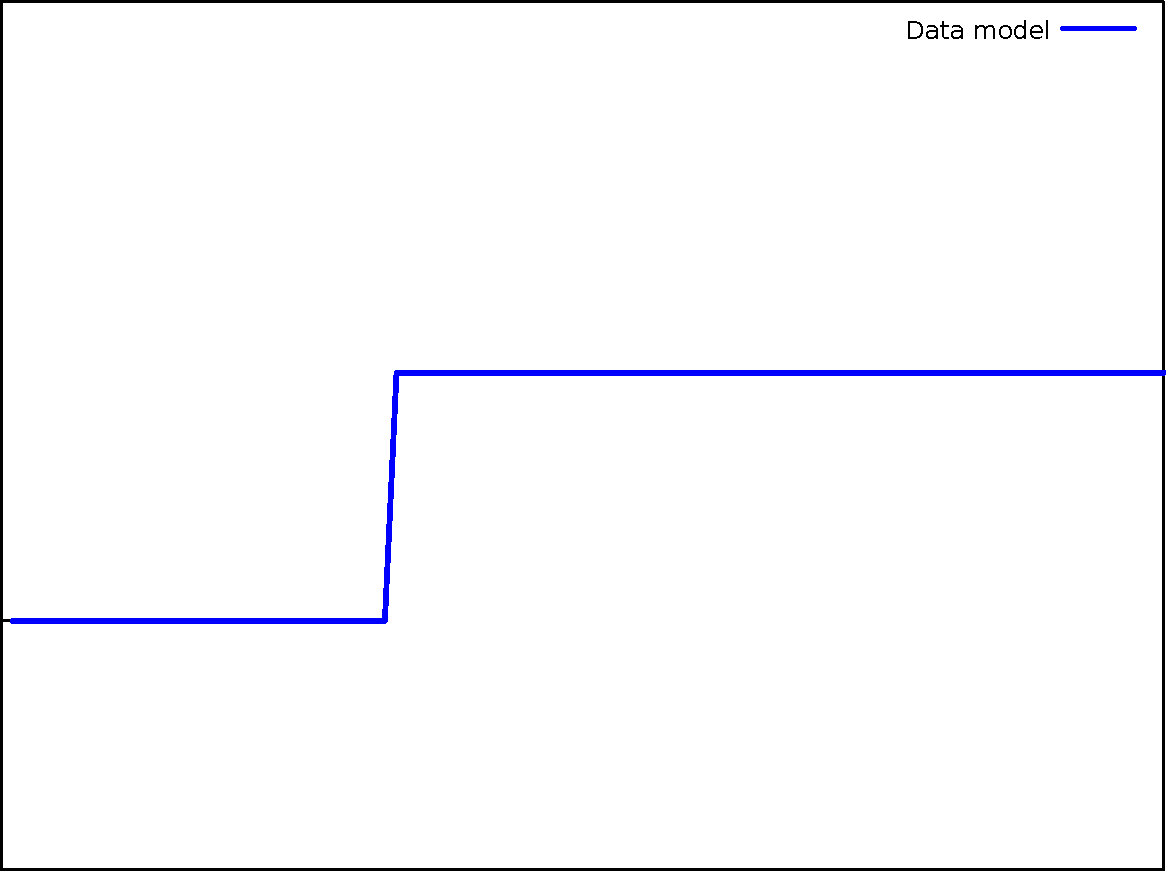
\includegraphics{images/data_bis.pdf}
      \end{axis}
      %% --------------------------------------------------------------------
          \end{tikzpicture}
          \end{figure}

      \columnbreak

      \begin{center}
        Target $\velocity$ Model
      \end{center}
      \vspace{-1.5cm}

      \begin{figure}
        \centering
          \begin{tikzpicture}
      \begin{axis}[%
          width=\plotwidth, height=\plotheight,,
          at={(0,0)},scale only axis,separate axis lines,xminorticks=true,
          xlabel={Depth},
          %ylabel={$\velocity$},
          %%   ymode=log,
          yminorticks=true,
          %%   xmin=0.,xmax=100.
        ]

        %% load current data
        %% -----------------
        \addplot[color=blue!50!black,mark options={solid},
          forget plot,line width=1pt,
          mark size=2pt]
        table[x=monx,y=mony]
        {images/VP100.dat};
      \end{axis}
      %% --------------------------------------------------------------------
          \end{tikzpicture}
          \end{figure}

      \end{multicols}

\end{frame}


%%%%%%%%%%%%%%%%%%%%%%%%%%%%%%%%%%%%%%%%%%%%% 1 %%%%%%%%%%%%%%%%%%%%%%%%%%%%%%%%%%%%%%%%%%%%%%%%
\begin{frame}{1D Preliminary tests :}
  \begin{multicols}{2}
    \normalsize
1D FWI :
\begin{itemize}
\item Lagrange / B-Bézier Operators
\item RK4 / AB3 time-schemes
\end{itemize}
\vspace{0.5cm}
\uncover<2->{
Adjoint test passed with :
\begin{itemize}
\item With a canonical space inner-product ($<u,v>_X=\sum_i u_iv_i$)
\item With a M-space inner product ($<u,v>_X^M=<Mu,v>_X$)
\end{itemize}}
\columnbreak
Gradient expression :
  \begin{equation}
     \nabla_{{\velocity}}\CF=-\int_0^{T} \int_{\Omega} \frac{2}{\density \velocity^3} \frac{\partial \contP}{\partial t}\Lbdun d\Omega dt
  \end{equation}
  \vspace{0.2cm}
  \\
  \tiny
  \uncover<2->{
\code{./run}\\
\code{----- Adjoint test -------}\\
\code{ inner product U/D   553123.57586755091    }\\
\code{ inner product G/Q   553123.57586756046    }\\
}
  %% ------------------------------------\\
  \uncover<3->{
\code{./run}\\
\code{----- Adjoint test -------}\\
\code{ inner product U/D  -75077.332007383695  }\\
\code{ inner product G/Q  -75077.332007386358  }\\
%------------------------------------\\
\code{./run}\\
\code{----- Adjoint test -------}\\
\code{ inner product U/D   125669.89223600870  }\\
\code{ inner product G/Q   125669.89223600952  }\\
}
%------------------------------------\\
\end{multicols}
\end{frame}
%%%%%%%%%%%%%%%%%%%%%%%%%%%%%%%%%%%%%%%%%%%%% 1 %%%%%%%%%%%%%%%%%%%%%%%%%%%%%%%%%%%%%%%%%%%%%%%%


%%%%%%%%%%%%%%%%%%%%%%%%%%%%%%%%%%%%%%%%%%%%% 2 %%%%%%%%%%%%%%%%%%%%%%%%%%%%%%%%%%%%%%%%%%%%%%%%
\begin{frame}{1D Velocity Model Reconstructions}
  \setlength{\plotwidth} {10.3cm}
  \setlength{\plotheight}{6cm}
  \begin{figure}
    \centering
    \begin{tikzpicture}

      \begin{axis}[width=\plotwidth,
                   height=\plotheight,
                   xlabel={Depth},
                   ylabel={$\velocity$},
                   legend pos=south east]
        \addplot[color=red!90!black,mark options={solid},
          line width=1pt,
          mark size=2pt]
        table[x=monx,y=mony]
        {images/VP_ATD.dat};
        \addlegendentry{Adjoint Then Discretize\footnote{With Bernstein-Bézier elements}}
        \addplot[color=blue!90!black,mark options={solid},
          line width=1pt,
          mark size=2pt]
        table[x=monx,y=mony]
        {images/VP_DTA.dat};
        \addlegendentry{Discretize Then Adjoint\footnote{With canonical scalar product}}
      \end{axis}
    \end{tikzpicture}
  \end{figure}
  \begin{center}
    $\velocity$ Model at the 100th FWI iteration
  \end{center}


\end{frame}


%%%%%%%%%%%%%%%%%%%%%%%%%%%%%%%%%%%%%%%%%%%%% 2 %%%%%%%%%%%%%%%%%%%%%%%%%%%%%%%%%%%%%%%%%%%%%%%%
\begin{frame}{1D Velocity Model Reconstructions}

  \begin{minipage}[top]{0.5\linewidth}
    With RK4 :
  \end{minipage}
  \begin{minipage}[top]{0.4\linewidth}
    ~~~~~~~~~~~~~~~ With AB3 :
  \end{minipage}
  \begin{minipage}[top]{0.5\linewidth}
    \setlength{\plotwidth} {6.0cm}
    \setlength{\plotheight}{5cm}
      \begin{figure}
        \begin{tikzpicture}
          \begin{axis}[width=\plotwidth,
              height=\plotheight,
              ymode = log,
              ylabel near ticks, yticklabel pos=right,
              xlabel={FWI Iterations},
              legend pos=north east]
            \addplot[color=red!90!black,mark options={solid},
              line width=1pt,
              mark size=2pt]
            table[x=monx,y=mony]
            {images/run_atd_rk4_bb.txt};
            \addlegendentry{AtD}
            \addplot[color=blue!90!black,mark options={solid},
              line width=1pt,
              mark size=2pt]
            table[x=monx,y=mony]
            {images/run_dta_rk4_bb.txt};
            \addlegendentry{DtA}
          \end{axis}
        \end{tikzpicture}
      \end{figure}
    \end{minipage}\hfill
    \begin{minipage}[top]{0.5\linewidth}
      \begin{figure}
        \begin{tikzpicture}
          \setlength{\plotwidth} {6.0cm}
          \setlength{\plotheight}{5cm}
          \begin{axis}[width=\plotwidth,
              height=\plotheight,
              xlabel={FWI Iterations},
              ymode = log,
              ylabel={log(Cost Function)},
%              ylabel style={rotate=-90},
              legend pos=north east]
            \addplot[color=red!90!black,mark options={solid},
              line width=1pt,
              mark size=2pt]
            table[x=monx,y=mony]
            {images/run_atd_ab3_bb.txt};
            \addlegendentry{AtD}
            \addplot[color=blue!90!black,mark options={solid},
              line width=1pt,
              mark size=2pt]
            table[x=monx,y=mony]
            {images/run_dta_ab3_bb.txt};
            \addlegendentry{DtA}
          \end{axis}
        \end{tikzpicture}
      \end{figure}
    \end{minipage}

    \uncover<2->{
    \begin{itemize}
      \item For RK4 scheme : Similar convergency
      \item For AB3 scheme : \textcolor{red}{AtD} is slighly better than \textcolor{blue}{DtA}
      \item The slope strongly depends on the optimizer -> Impossibilty to conclude
    \end{itemize}
    }

\end{frame}

%%%%%%%%%%%%%%%%%%%%%%%%%%%%%%%%%%%%%%%%%%%%%%%%%%%%%%%%%%%%%%%%%%%%%%%%
\subsection{2D Time Domain FWI Results}
\begin{frame}{2D Time Domain Reconstruction}

2D FWI :
\begin{itemize}
\item Developped in Total environnement (DIP\footnote{\url{http://dip.inria.fr/}})
\item Nodal Space Operators (Lagrangian/Jacobian)
\item Modal Space Operators (Bernstein-Bézier)
\item Runge Kutta 2/4 and Adams Bashforth time-schemes
\end{itemize}
\vspace{0.5cm}
Discretize Then Adjoint strategy not implemented :
\begin{itemize}
\item Tremendous task in a complex industrial code
\end{itemize}
%% \columnbreak
%% \uncover<2->{
%% Gradient expression :
%%   \begin{equation}
%%      \nabla_{{\velocity}}J=-\int_0^{T} \int_{\Omega} \frac{2}{\density \velocity^3} \frac{\partial \contP}{\partial t}\Lbdun d\Omega dt.
%%   \end{equation}
\end{frame}


\begin{frame}[noframenumbering]{2D Time Domain Reconstruction}

2D FWI :
\begin{itemize}
\item Developped in Total environnement (DIP\footnote{\url{http://dip.inria.fr/}})
\item Nodal Operators (Lagrangian/Jacobian)
\item Modal Operators (Bernstein-Bézier)
\item Runge Kutta 2/4 and Adams Bashforth time-schemes
\end{itemize}
\vspace{0.5cm}
 Gradient expression :
  \begin{equation}
     \nabla_{\boldsymbol{\textcolor{\mygreen}{\frac{1}{\kappa}}}}\CF=\int_0^{T} \int_{\Omega} \frac{\partial \contP}{\partial t}\Lbdun d\Omega dt \text{~~~~ with : } \boldsymbol{\textcolor{\mygreen}{\kappa}}=\density \velocity^2
  \end{equation}
   $\velocity$, $\density$ and  $\boldsymbol{\textcolor{\mygreen}{\kappa}}$  Constant per elements
\end{frame}

\newlength{\modelwidth}
\setlength{\modelwidth}{10.8cm}
\newcommand{\modeltitle}{Initial $\velocity$ Model}

\begin{frame}{2D Time Domain FWI Reconstructions}{Time-schemes comparison}
  \vspace{-0.5cm}
  \renewcommand{\modelfile}{fig/marmousi_noise_ini}
  \begin{figure}
       \begin{tikzpicture}
\pgfmathsetmacro{\xmin} {0.}
\pgfmathsetmacro{\xmax} {12.}
\pgfmathsetmacro{\zmin} {0.}
\pgfmathsetmacro{\zmax} {2.5}

\begin{axis}[%
title={\small{\modeltitle}},
width=1.0\modelwidth,
height=0.4\modelwidth,
axis on top, separate axis lines,
xmin=\xmin, xmax=\xmax, %xlabel={x (km)},
ymin=\zmin, ymax=\zmax, ylabel={depth (km)},
yticklabels={},xticklabels={},
y dir=reverse,
colormap/paraview, colorbar,
point meta min=1.5e-3, point meta max=5.5e-3,
colorbar/width=2.5mm,
]
\addplot [forget plot] graphics [xmin=\xmin,xmax=\xmax,ymin=\zmin,ymax=\zmax] {{\modelfile}.png};
\end{axis}
\end{tikzpicture}%
 \hfill
  \end{figure}
  \vspace{-1cm}
  \renewcommand{\modeltitle}{Target $\velocity$ Model}
  \renewcommand{\modelfile}{fig/marmousi_target}
  \begin{figure}
       \begin{tikzpicture}
\pgfmathsetmacro{\xmin} {0.}
\pgfmathsetmacro{\xmax} {12.}
\pgfmathsetmacro{\zmin} {0.}
\pgfmathsetmacro{\zmax} {2.5}

\begin{axis}[%
title={\small{\modeltitle}},
width=1.0\modelwidth,
height=0.4\modelwidth,
axis on top, separate axis lines,
xmin=\xmin, xmax=\xmax, %xlabel={x (km)},
ymin=\zmin, ymax=\zmax, ylabel={depth (km)},
yticklabels={},xticklabels={},
y dir=reverse,
colormap/paraview, colorbar,
point meta min=1.5e-3, point meta max=5.5e-3,
colorbar/width=2.5mm,
]
\addplot [forget plot] graphics [xmin=\xmin,xmax=\xmax,ymin=\zmin,ymax=\zmax] {{\modelfile}.png};
\end{axis}
\end{tikzpicture}%
 \hfill
   \end{figure}
\end{frame}

\begin{frame}[noframenumbering]{2D Time Domain FWI Reconstructions}{Time-schemes comparison}
  \vspace{-0.5cm}
  \renewcommand{\modelfile}{fig/marmousi_noise_rk2}
  \renewcommand{\modeltitle}{\textbf{\textcolor{red}{RK2}} Reconstructed $\velocity$ Model (30 iterations)}
  \begin{figure}
    \begin{tikzpicture}
\pgfmathsetmacro{\xmin} {0.}
\pgfmathsetmacro{\xmax} {12.}
\pgfmathsetmacro{\zmin} {0.}
\pgfmathsetmacro{\zmax} {2.5}

\begin{axis}[%
title={\small{\modeltitle}},
width=1.0\modelwidth,
height=0.4\modelwidth,
axis on top, separate axis lines,
xmin=\xmin, xmax=\xmax, %xlabel={x (km)},
ymin=\zmin, ymax=\zmax, ylabel={depth (km)},
yticklabels={},xticklabels={},
y dir=reverse,
colormap/paraview, colorbar,
point meta min=1.5e-3, point meta max=5.5e-3,
colorbar/width=2.5mm,
]
\addplot [forget plot] graphics [xmin=\xmin,xmax=\xmax,ymin=\zmin,ymax=\zmax] {{\modelfile}.png};
\end{axis}
\end{tikzpicture}%
 \hfill
  \end{figure}
  \vspace{-1cm}
  \renewcommand{\modeltitle}{Target $\velocity$ Model}
  \renewcommand{\modelfile}{fig/marmousi_target}
  \begin{figure}
    \begin{tikzpicture}
\pgfmathsetmacro{\xmin} {0.}
\pgfmathsetmacro{\xmax} {12.}
\pgfmathsetmacro{\zmin} {0.}
\pgfmathsetmacro{\zmax} {2.5}

\begin{axis}[%
title={\small{\modeltitle}},
width=1.0\modelwidth,
height=0.4\modelwidth,
axis on top, separate axis lines,
xmin=\xmin, xmax=\xmax, %xlabel={x (km)},
ymin=\zmin, ymax=\zmax, ylabel={depth (km)},
yticklabels={},xticklabels={},
y dir=reverse,
colormap/paraview, colorbar,
point meta min=1.5e-3, point meta max=5.5e-3,
colorbar/width=2.5mm,
]
\addplot [forget plot] graphics [xmin=\xmin,xmax=\xmax,ymin=\zmin,ymax=\zmax] {{\modelfile}.png};
\end{axis}
\end{tikzpicture}%
 \hfill
  \end{figure}
\end{frame}

\begin{frame}[noframenumbering]{2D Time Domain FWI Reconstructions}{Time-schemes comparison}
  \vspace{-0.5cm}
  \renewcommand{\modelfile}{fig/marmousi_noise_rk4_2}
  \renewcommand{\modeltitle}{\textbf{\textcolor{red}{RK4}} Reconstructed $\velocity$ Model (30 iterations)}
  \begin{figure}
    \begin{tikzpicture}
\pgfmathsetmacro{\xmin} {0.}
\pgfmathsetmacro{\xmax} {12.}
\pgfmathsetmacro{\zmin} {0.}
\pgfmathsetmacro{\zmax} {2.5}

\begin{axis}[%
title={\small{\modeltitle}},
width=1.0\modelwidth,
height=0.4\modelwidth,
axis on top, separate axis lines,
xmin=\xmin, xmax=\xmax, %xlabel={x (km)},
ymin=\zmin, ymax=\zmax, ylabel={depth (km)},
yticklabels={},xticklabels={},
y dir=reverse,
colormap/paraview, colorbar,
point meta min=1.5e-3, point meta max=5.5e-3,
colorbar/width=2.5mm,
]
\addplot [forget plot] graphics [xmin=\xmin,xmax=\xmax,ymin=\zmin,ymax=\zmax] {{\modelfile}.png};
\end{axis}
\end{tikzpicture}%
 \hfill
  \end{figure}
  \vspace{-1cm}
  \renewcommand{\modeltitle}{Target $\velocity$ Model}
  \renewcommand{\modelfile}{fig/marmousi_target}
  \begin{figure}
    \begin{tikzpicture}
\pgfmathsetmacro{\xmin} {0.}
\pgfmathsetmacro{\xmax} {12.}
\pgfmathsetmacro{\zmin} {0.}
\pgfmathsetmacro{\zmax} {2.5}

\begin{axis}[%
title={\small{\modeltitle}},
width=1.0\modelwidth,
height=0.4\modelwidth,
axis on top, separate axis lines,
xmin=\xmin, xmax=\xmax, %xlabel={x (km)},
ymin=\zmin, ymax=\zmax, ylabel={depth (km)},
yticklabels={},xticklabels={},
y dir=reverse,
colormap/paraview, colorbar,
point meta min=1.5e-3, point meta max=5.5e-3,
colorbar/width=2.5mm,
]
\addplot [forget plot] graphics [xmin=\xmin,xmax=\xmax,ymin=\zmin,ymax=\zmax] {{\modelfile}.png};
\end{axis}
\end{tikzpicture}%
 \hfill
  \end{figure}
\end{frame}


\begin{frame}[noframenumbering]{2D Time Domain FWI Reconstructions}{Time-schemes comparison}
  \vspace{-0.5cm}
  \renewcommand{\modelfile}{fig/marmousi_noise_ab3}
  \renewcommand{\modeltitle}{\textbf{\textcolor{red}{AB3}} Reconstructed $\velocity$ Model (30 iterations)}
  \begin{figure}
       \begin{tikzpicture}
\pgfmathsetmacro{\xmin} {0.}
\pgfmathsetmacro{\xmax} {12.}
\pgfmathsetmacro{\zmin} {0.}
\pgfmathsetmacro{\zmax} {2.5}

\begin{axis}[%
title={\small{\modeltitle}},
width=1.0\modelwidth,
height=0.4\modelwidth,
axis on top, separate axis lines,
xmin=\xmin, xmax=\xmax, %xlabel={x (km)},
ymin=\zmin, ymax=\zmax, ylabel={depth (km)},
yticklabels={},xticklabels={},
y dir=reverse,
colormap/paraview, colorbar,
point meta min=1.5e-3, point meta max=5.5e-3,
colorbar/width=2.5mm,
]
\addplot [forget plot] graphics [xmin=\xmin,xmax=\xmax,ymin=\zmin,ymax=\zmax] {{\modelfile}.png};
\end{axis}
\end{tikzpicture}%
 \hfill
  \end{figure}
  \vspace{-1cm}
  \renewcommand{\modeltitle}{Target $\velocity$ Model}
  \renewcommand{\modelfile}{fig/marmousi_target}
  \begin{figure}
       \begin{tikzpicture}
\pgfmathsetmacro{\xmin} {0.}
\pgfmathsetmacro{\xmax} {12.}
\pgfmathsetmacro{\zmin} {0.}
\pgfmathsetmacro{\zmax} {2.5}

\begin{axis}[%
title={\small{\modeltitle}},
width=1.0\modelwidth,
height=0.4\modelwidth,
axis on top, separate axis lines,
xmin=\xmin, xmax=\xmax, %xlabel={x (km)},
ymin=\zmin, ymax=\zmax, ylabel={depth (km)},
yticklabels={},xticklabels={},
y dir=reverse,
colormap/paraview, colorbar,
point meta min=1.5e-3, point meta max=5.5e-3,
colorbar/width=2.5mm,
]
\addplot [forget plot] graphics [xmin=\xmin,xmax=\xmax,ymin=\zmin,ymax=\zmax] {{\modelfile}.png};
\end{axis}
\end{tikzpicture}%
 \hfill
   \end{figure}
\end{frame}

\begin{frame}{2D Time Domain FWI Reconstructions}{Nodal/Modal Comparison}

  \begin{multicols}{2}
    \begin{itemize}
    \item 47k P1 elements
    \item Time Scheme : AB3
    \item Constant $\density$ model ($\density=1$)
    \item 19 sources / 181 Receivers
    \item 30 iterations
    \item 120 cores
    \item Nodal computation time : 5h10
    \item Modal computation time : 7h10$^{[1]}$
    \end{itemize}
    \columnbreak

    \setlength{\plotwidth} {6.0cm}
    \setlength{\plotheight}{5cm}
    Cost function evolution :
   \begin{figure}
        \begin{tikzpicture}
          \begin{axis}[width=\plotwidth,
              height=\plotheight,
%              ymode = log,
              xlabel={FWI Iterations},
              legend pos=north east]
            \addplot[color=red!90!black,mark options={solid},
              line width=1pt,
              mark size=2pt]
            table[x=monx,y=mony]
            {fig/run_ab3_lag.txt};
            \addlegendentry{Nodal}
            \addplot[mark=*,color=blue!90!black,mark options={scale=0.7},
              line width=0pt,
              mark size=2pt]
            table[x=monx,y=mony]
            {fig/run_ab3_lag.txt};
            \addlegendentry{Modal}
          \end{axis}
        \end{tikzpicture}
      \end{figure}
  \end{multicols}

  %% pour mettre en bas et en petit
  \vfill
  \tiny
  %%%%%%%%%%%%%%%%%%%%%%%%%%%%%%%%%%
  \begin{thebibliography}{1}
  \bibitem{chan2017gpu} Chan J. and Warburton T.
    \newblock GPU-Accelerated Bernstein Bézier Discontinuous Galerkin Methods for Wave Problems
    \newblock SIAM Journal on Scientific Computing 2017
  \end{thebibliography}

\end{frame}

\subsection{2D Multiscale Reconstruction}
\begin{frame}{2D Multiscale Reconstructions}{Reconstruction with an initial smooth model}
  \vspace{-0.5cm}
  \renewcommand{\modelfile}{fig/marmousi_filter_0}
  \renewcommand{\modeltitle}{Initial $\velocity$ Model}
  \begin{figure}
       \begin{tikzpicture}
\pgfmathsetmacro{\xmin} {0.}
\pgfmathsetmacro{\xmax} {12.}
\pgfmathsetmacro{\zmin} {0.}
\pgfmathsetmacro{\zmax} {2.5}

\begin{axis}[%
title={\small{\modeltitle}},
width=1.0\modelwidth,
height=0.4\modelwidth,
axis on top, separate axis lines,
xmin=\xmin, xmax=\xmax, %xlabel={x (km)},
ymin=\zmin, ymax=\zmax, ylabel={depth (km)},
yticklabels={},xticklabels={},
y dir=reverse,
colormap/paraview, colorbar,
point meta min=1.5e-3, point meta max=5.5e-3,
colorbar/width=2.5mm,
]
\addplot [forget plot] graphics [xmin=\xmin,xmax=\xmax,ymin=\zmin,ymax=\zmax] {{\modelfile}.png};
\end{axis}
\end{tikzpicture}%
 \hfill
  \end{figure}
  \vspace{-1cm}
  \renewcommand{\modeltitle}{Target $\velocity$ Model}
  \renewcommand{\modelfile}{fig/marmousi_target}
  \begin{figure}
       \begin{tikzpicture}
\pgfmathsetmacro{\xmin} {0.}
\pgfmathsetmacro{\xmax} {12.}
\pgfmathsetmacro{\zmin} {0.}
\pgfmathsetmacro{\zmax} {2.5}

\begin{axis}[%
title={\small{\modeltitle}},
width=1.0\modelwidth,
height=0.4\modelwidth,
axis on top, separate axis lines,
xmin=\xmin, xmax=\xmax, %xlabel={x (km)},
ymin=\zmin, ymax=\zmax, ylabel={depth (km)},
yticklabels={},xticklabels={},
y dir=reverse,
colormap/paraview, colorbar,
point meta min=1.5e-3, point meta max=5.5e-3,
colorbar/width=2.5mm,
]
\addplot [forget plot] graphics [xmin=\xmin,xmax=\xmax,ymin=\zmin,ymax=\zmax] {{\modelfile}.png};
\end{axis}
\end{tikzpicture}%
 \hfill
   \end{figure}
\end{frame}

\begin{frame}[noframenumbering]{2D Multiscale Reconstructions}{Reconstruction with an initial smooth model}
  \vspace{-0.5cm}
  \renewcommand{\modelfile}{fig/marmousi_nofilter}
  \renewcommand{\modeltitle}{Reconstructed model $\velocity$ Model (30 iterations AB3)}
  \begin{figure}
       \begin{tikzpicture}
\pgfmathsetmacro{\xmin} {0.}
\pgfmathsetmacro{\xmax} {12.}
\pgfmathsetmacro{\zmin} {0.}
\pgfmathsetmacro{\zmax} {2.5}

\begin{axis}[%
title={\small{\modeltitle}},
width=1.0\modelwidth,
height=0.4\modelwidth,
axis on top, separate axis lines,
xmin=\xmin, xmax=\xmax, %xlabel={x (km)},
ymin=\zmin, ymax=\zmax, ylabel={depth (km)},
yticklabels={},xticklabels={},
y dir=reverse,
colormap/paraview, colorbar,
point meta min=1.5e-3, point meta max=5.5e-3,
colorbar/width=2.5mm,
]
\addplot [forget plot] graphics [xmin=\xmin,xmax=\xmax,ymin=\zmin,ymax=\zmax] {{\modelfile}.png};
\end{axis}
\end{tikzpicture}%
 \hfill
  \end{figure}
  \vspace{-1cm}
  \renewcommand{\modeltitle}{Target $\velocity$ Model}
  \renewcommand{\modelfile}{fig/marmousi_target}
  \begin{figure}
       \begin{tikzpicture}
\pgfmathsetmacro{\xmin} {0.}
\pgfmathsetmacro{\xmax} {12.}
\pgfmathsetmacro{\zmin} {0.}
\pgfmathsetmacro{\zmax} {2.5}

\begin{axis}[%
title={\small{\modeltitle}},
width=1.0\modelwidth,
height=0.4\modelwidth,
axis on top, separate axis lines,
xmin=\xmin, xmax=\xmax, %xlabel={x (km)},
ymin=\zmin, ymax=\zmax, ylabel={depth (km)},
yticklabels={},xticklabels={},
y dir=reverse,
colormap/paraview, colorbar,
point meta min=1.5e-3, point meta max=5.5e-3,
colorbar/width=2.5mm,
]
\addplot [forget plot] graphics [xmin=\xmin,xmax=\xmax,ymin=\zmin,ymax=\zmax] {{\modelfile}.png};
\end{axis}
\end{tikzpicture}%
 \hfill
   \end{figure}
\end{frame}



\begin{frame}{2D Multiscale Reconstructions}{Multiscale Principle}


  \setlength{\plotwidth} {6.0cm}
  \setlength{\plotheight}{3cm}
  \begin{figure}
    \begin{tikzpicture}
      \begin{axis}[width=\plotwidth,
          height=\plotheight,
          %              ymode = log,
          xlabel={FWI Iterations},
          ymin=-5,ymax=29
        ]
        \addplot[color=red!90!black,mark options={solid},
          line width=1pt,
          mark size=2pt]
        table[x=monx,y=mony]
        {fig/file1.txt};
      \end{axis}
    \end{tikzpicture}
  \end{figure}

  \begin{figure}
    \begin{tikzpicture}
      \begin{axis}[width=\plotwidth,
          height=\plotheight,
          %              ymode = log,
          xlabel={FWI Iterations},
        ]
        \addplot[color=red!90!black,mark options={solid},
          line width=1pt,
          mark size=2pt]
        table[x=monx,y=mony]
        {fig/file2.txt};
      \end{axis}
    \end{tikzpicture}
  \end{figure}


  \begin{figure}
    \begin{tikzpicture}
      \begin{axis}[width=\plotwidth,
          height=\plotheight,
          %              ymode = log,
          xlabel={FWI Iterations},
        ]
        \addplot[color=red!90!black,mark options={solid},
          line width=1pt,
          mark size=2pt]
        table[x=monx,y=mony]
        {fig/file3.txt};
      \end{axis}
    \end{tikzpicture}
  \end{figure}

\end{frame}


\begin{frame}{2D Multiscale Reconstructions}{Reconstruction with an initial smooth model}
  \vspace{-0.5cm}
  \renewcommand{\modelfile}{fig/marmousi_filter_0}
  \renewcommand{\modeltitle}{Initial $\velocity$ Model}
  \begin{figure}
       \begin{tikzpicture}
\pgfmathsetmacro{\xmin} {0.}
\pgfmathsetmacro{\xmax} {12.}
\pgfmathsetmacro{\zmin} {0.}
\pgfmathsetmacro{\zmax} {2.5}

\begin{axis}[%
title={\small{\modeltitle}},
width=1.0\modelwidth,
height=0.4\modelwidth,
axis on top, separate axis lines,
xmin=\xmin, xmax=\xmax, %xlabel={x (km)},
ymin=\zmin, ymax=\zmax, ylabel={depth (km)},
yticklabels={},xticklabels={},
y dir=reverse,
colormap/paraview, colorbar,
point meta min=1.5e-3, point meta max=5.5e-3,
colorbar/width=2.5mm,
]
\addplot [forget plot] graphics [xmin=\xmin,xmax=\xmax,ymin=\zmin,ymax=\zmax] {{\modelfile}.png};
\end{axis}
\end{tikzpicture}%
 \hfill
  \end{figure}
  \vspace{-1cm}
  \renewcommand{\modeltitle}{Target $\velocity$ Model}
  \renewcommand{\modelfile}{fig/marmousi_target}
  \begin{figure}
       \begin{tikzpicture}
\pgfmathsetmacro{\xmin} {0.}
\pgfmathsetmacro{\xmax} {12.}
\pgfmathsetmacro{\zmin} {0.}
\pgfmathsetmacro{\zmax} {2.5}

\begin{axis}[%
title={\small{\modeltitle}},
width=1.0\modelwidth,
height=0.4\modelwidth,
axis on top, separate axis lines,
xmin=\xmin, xmax=\xmax, %xlabel={x (km)},
ymin=\zmin, ymax=\zmax, ylabel={depth (km)},
yticklabels={},xticklabels={},
y dir=reverse,
colormap/paraview, colorbar,
point meta min=1.5e-3, point meta max=5.5e-3,
colorbar/width=2.5mm,
]
\addplot [forget plot] graphics [xmin=\xmin,xmax=\xmax,ymin=\zmin,ymax=\zmax] {{\modelfile}.png};
\end{axis}
\end{tikzpicture}%
 \hfill
   \end{figure}
\end{frame}

\begin{frame}[noframenumbering]{2D Multiscale Reconstructions}{Reconstruction with an initial smooth model}
  \vspace{-0.5cm}
  \renewcommand{\modelfile}{fig/marmousi_filter_1}
  \renewcommand{\modeltitle}{Reconstructed $\velocity$ Model with \textcolor{red}{1.0-2.5Hz} filter}
  \begin{figure}
       \begin{tikzpicture}
\pgfmathsetmacro{\xmin} {0.}
\pgfmathsetmacro{\xmax} {12.}
\pgfmathsetmacro{\zmin} {0.}
\pgfmathsetmacro{\zmax} {2.5}

\begin{axis}[%
title={\small{\modeltitle}},
width=1.0\modelwidth,
height=0.4\modelwidth,
axis on top, separate axis lines,
xmin=\xmin, xmax=\xmax, %xlabel={x (km)},
ymin=\zmin, ymax=\zmax, ylabel={depth (km)},
yticklabels={},xticklabels={},
y dir=reverse,
colormap/paraview, colorbar,
point meta min=1.5e-3, point meta max=5.5e-3,
colorbar/width=2.5mm,
]
\addplot [forget plot] graphics [xmin=\xmin,xmax=\xmax,ymin=\zmin,ymax=\zmax] {{\modelfile}.png};
\end{axis}
\end{tikzpicture}%
 \hfill
  \end{figure}
  \vspace{-1cm}
  \renewcommand{\modeltitle}{Target $\velocity$ Model}
  \renewcommand{\modelfile}{fig/marmousi_target}
  \begin{figure}
       \begin{tikzpicture}
\pgfmathsetmacro{\xmin} {0.}
\pgfmathsetmacro{\xmax} {12.}
\pgfmathsetmacro{\zmin} {0.}
\pgfmathsetmacro{\zmax} {2.5}

\begin{axis}[%
title={\small{\modeltitle}},
width=1.0\modelwidth,
height=0.4\modelwidth,
axis on top, separate axis lines,
xmin=\xmin, xmax=\xmax, %xlabel={x (km)},
ymin=\zmin, ymax=\zmax, ylabel={depth (km)},
yticklabels={},xticklabels={},
y dir=reverse,
colormap/paraview, colorbar,
point meta min=1.5e-3, point meta max=5.5e-3,
colorbar/width=2.5mm,
]
\addplot [forget plot] graphics [xmin=\xmin,xmax=\xmax,ymin=\zmin,ymax=\zmax] {{\modelfile}.png};
\end{axis}
\end{tikzpicture}%
 \hfill
   \end{figure}
\end{frame}

\begin{frame}[noframenumbering]{2D Multiscale Reconstructions}{Reconstruction with an initial smooth model}
  \vspace{-0.5cm}
  \renewcommand{\modelfile}{fig/marmousi_filter_2}
  \renewcommand{\modeltitle}{Reconstructed $\velocity$ Model with \textcolor{red}{1.0-7.5Hz} filter}
  \begin{figure}
       \begin{tikzpicture}
\pgfmathsetmacro{\xmin} {0.}
\pgfmathsetmacro{\xmax} {12.}
\pgfmathsetmacro{\zmin} {0.}
\pgfmathsetmacro{\zmax} {2.5}

\begin{axis}[%
title={\small{\modeltitle}},
width=1.0\modelwidth,
height=0.4\modelwidth,
axis on top, separate axis lines,
xmin=\xmin, xmax=\xmax, %xlabel={x (km)},
ymin=\zmin, ymax=\zmax, ylabel={depth (km)},
yticklabels={},xticklabels={},
y dir=reverse,
colormap/paraview, colorbar,
point meta min=1.5e-3, point meta max=5.5e-3,
colorbar/width=2.5mm,
]
\addplot [forget plot] graphics [xmin=\xmin,xmax=\xmax,ymin=\zmin,ymax=\zmax] {{\modelfile}.png};
\end{axis}
\end{tikzpicture}%
 \hfill
  \end{figure}
  \vspace{-1cm}
  \renewcommand{\modeltitle}{Target $\velocity$ Model}
  \renewcommand{\modelfile}{fig/marmousi_target}
  \begin{figure}
       \begin{tikzpicture}
\pgfmathsetmacro{\xmin} {0.}
\pgfmathsetmacro{\xmax} {12.}
\pgfmathsetmacro{\zmin} {0.}
\pgfmathsetmacro{\zmax} {2.5}

\begin{axis}[%
title={\small{\modeltitle}},
width=1.0\modelwidth,
height=0.4\modelwidth,
axis on top, separate axis lines,
xmin=\xmin, xmax=\xmax, %xlabel={x (km)},
ymin=\zmin, ymax=\zmax, ylabel={depth (km)},
yticklabels={},xticklabels={},
y dir=reverse,
colormap/paraview, colorbar,
point meta min=1.5e-3, point meta max=5.5e-3,
colorbar/width=2.5mm,
]
\addplot [forget plot] graphics [xmin=\xmin,xmax=\xmax,ymin=\zmin,ymax=\zmax] {{\modelfile}.png};
\end{axis}
\end{tikzpicture}%
 \hfill
   \end{figure}
\end{frame}

\begin{frame}[noframenumbering]{2D Multiscale Reconstructions}{Reconstruction with an initial smooth model}
  \vspace{-0.5cm}
  \renewcommand{\modelfile}{fig/marmousi_filter_3}
  \renewcommand{\modeltitle}{Reconstructed $\velocity$ Model with \textcolor{red}{1.0-10Hz} filter}
  \begin{figure}
       \begin{tikzpicture}
\pgfmathsetmacro{\xmin} {0.}
\pgfmathsetmacro{\xmax} {12.}
\pgfmathsetmacro{\zmin} {0.}
\pgfmathsetmacro{\zmax} {2.5}

\begin{axis}[%
title={\small{\modeltitle}},
width=1.0\modelwidth,
height=0.4\modelwidth,
axis on top, separate axis lines,
xmin=\xmin, xmax=\xmax, %xlabel={x (km)},
ymin=\zmin, ymax=\zmax, ylabel={depth (km)},
yticklabels={},xticklabels={},
y dir=reverse,
colormap/paraview, colorbar,
point meta min=1.5e-3, point meta max=5.5e-3,
colorbar/width=2.5mm,
]
\addplot [forget plot] graphics [xmin=\xmin,xmax=\xmax,ymin=\zmin,ymax=\zmax] {{\modelfile}.png};
\end{axis}
\end{tikzpicture}%
 \hfill
  \end{figure}
  \vspace{-1cm}
  \renewcommand{\modeltitle}{Target $\velocity$ Model}
  \renewcommand{\modelfile}{fig/marmousi_target}
  \begin{figure}
       \begin{tikzpicture}
\pgfmathsetmacro{\xmin} {0.}
\pgfmathsetmacro{\xmax} {12.}
\pgfmathsetmacro{\zmin} {0.}
\pgfmathsetmacro{\zmax} {2.5}

\begin{axis}[%
title={\small{\modeltitle}},
width=1.0\modelwidth,
height=0.4\modelwidth,
axis on top, separate axis lines,
xmin=\xmin, xmax=\xmax, %xlabel={x (km)},
ymin=\zmin, ymax=\zmax, ylabel={depth (km)},
yticklabels={},xticklabels={},
y dir=reverse,
colormap/paraview, colorbar,
point meta min=1.5e-3, point meta max=5.5e-3,
colorbar/width=2.5mm,
]
\addplot [forget plot] graphics [xmin=\xmin,xmax=\xmax,ymin=\zmin,ymax=\zmax] {{\modelfile}.png};
\end{axis}
\end{tikzpicture}%
 \hfill
   \end{figure}
\end{frame}

\begin{frame}[noframenumbering]{2D Multiscale Reconstructions}{Reconstruction with an initial smooth model}
  \vspace{-0.5cm}
  \renewcommand{\modelfile}{fig/marmousi_filter_5}
  \renewcommand{\modeltitle}{Reconstructed $\velocity$ Model with \textcolor{red}{1.0-15Hz} filter}
  \begin{figure}
       \begin{tikzpicture}
\pgfmathsetmacro{\xmin} {0.}
\pgfmathsetmacro{\xmax} {12.}
\pgfmathsetmacro{\zmin} {0.}
\pgfmathsetmacro{\zmax} {2.5}

\begin{axis}[%
title={\small{\modeltitle}},
width=1.0\modelwidth,
height=0.4\modelwidth,
axis on top, separate axis lines,
xmin=\xmin, xmax=\xmax, %xlabel={x (km)},
ymin=\zmin, ymax=\zmax, ylabel={depth (km)},
yticklabels={},xticklabels={},
y dir=reverse,
colormap/paraview, colorbar,
point meta min=1.5e-3, point meta max=5.5e-3,
colorbar/width=2.5mm,
]
\addplot [forget plot] graphics [xmin=\xmin,xmax=\xmax,ymin=\zmin,ymax=\zmax] {{\modelfile}.png};
\end{axis}
\end{tikzpicture}%
 \hfill
  \end{figure}
  \vspace{-1cm}
  \renewcommand{\modeltitle}{Target $\velocity$ Model}
  \renewcommand{\modelfile}{fig/marmousi_target}
  \begin{figure}
       \begin{tikzpicture}
\pgfmathsetmacro{\xmin} {0.}
\pgfmathsetmacro{\xmax} {12.}
\pgfmathsetmacro{\zmin} {0.}
\pgfmathsetmacro{\zmax} {2.5}

\begin{axis}[%
title={\small{\modeltitle}},
width=1.0\modelwidth,
height=0.4\modelwidth,
axis on top, separate axis lines,
xmin=\xmin, xmax=\xmax, %xlabel={x (km)},
ymin=\zmin, ymax=\zmax, ylabel={depth (km)},
yticklabels={},xticklabels={},
y dir=reverse,
colormap/paraview, colorbar,
point meta min=1.5e-3, point meta max=5.5e-3,
colorbar/width=2.5mm,
]
\addplot [forget plot] graphics [xmin=\xmin,xmax=\xmax,ymin=\zmin,ymax=\zmax] {{\modelfile}.png};
\end{axis}
\end{tikzpicture}%
 \hfill
   \end{figure}
\end{frame}


\begin{frame}{2D Multiscale Reconstructions}

  \begin{multicols}{2}
    \begin{itemize}
    \item 47k P1 elements
    \item Time Scheme : AB3
    \item Constant $\density$ model ($\density=1$)
    \item 19 sources / 181 Receivers
    \item 120 cores
    \item Computation time : 17h
    \item Frequencies : \textcolor{red}{1-2.5Hz} \\ ~ \\ ~
    \end{itemize}
    \columnbreak

    \setlength{\plotwidth} {6.0cm}
    \setlength{\plotheight}{5cm}
    Cost function evolution :
    \begin{figure}
      \begin{tikzpicture}
        \begin{axis}[width=\plotwidth,
            height=\plotheight,
%            ymode = log,
            xlabel={FWI Iterations},
            xmin=-5.0, xmax=105.0,
            legend pos=south east]
          \addplot[color=red!90!black,mark options={solid},
            line width=1pt,
            mark size=2pt]
          table[x=monx,y=mony]
          {fig/run_marmousi_smooth.txt};
          \addlegendentry{$\CF(m)$}
        \end{axis}
      \end{tikzpicture}
    \end{figure}
  \end{multicols}
\end{frame}

\begin{frame}[noframenumbering]{2D Multiscale Reconstructions}

  \begin{multicols}{2}
    \begin{itemize}
    \item 47k P1 elements
    \item Time Scheme : AB3
    \item Constant $\density$ model ($\density=1$)
    \item 19 sources / 181 Receivers
    \item 120 cores
    \item Computation time : 17h
    \item Frequencies : 1-2.5Hz / \textcolor{red}{1-5Hz} \\ ~
    \end{itemize}
    \columnbreak

    \setlength{\plotwidth} {6.0cm}
    \setlength{\plotheight}{5cm}
    Cost function evolution :
    \begin{figure}
      \begin{tikzpicture}
        \begin{axis}[width=\plotwidth,
            height=\plotheight,
%            ymode = log,
            xlabel={FWI Iterations},
            xmin=-5.0, xmax=105.0,
            legend pos=south east]
          \addplot[color=red!90!black,mark options={solid},
            line width=1pt,
            mark size=2pt]
          table[x=monx,y=mony]
          {fig/run_marmousi_smooth_2.txt};
          \addlegendentry{$\CF(m)$}
        \end{axis}
      \end{tikzpicture}
    \end{figure}
  \end{multicols}
\end{frame}

\begin{frame}[noframenumbering]{2D Multiscale Reconstructions}

  \begin{multicols}{2}
    \begin{itemize}
    \item 47k P1 elements
    \item Time Scheme : AB3
    \item Constant $\density$ model ($\density=1$)
    \item 19 sources / 181 Receivers
    \item 120 cores
    \item Computation time : 17h
    \item Frequencies : 1-2.5Hz / 1-5Hz / \textcolor{red}{1-7.5Hz} \\ ~
    \end{itemize}
    \columnbreak

    \setlength{\plotwidth} {6.0cm}
    \setlength{\plotheight}{5cm}
    Cost function evolution :
    \begin{figure}
      \begin{tikzpicture}
        \begin{axis}[width=\plotwidth,
            height=\plotheight,
%            ymode = log,
            xlabel={FWI Iterations},
            xmin=-5.0, xmax=105.0,
            legend pos=south east]
          \addplot[color=red!90!black,mark options={solid},
            line width=1pt,
            mark size=2pt]
          table[x=monx,y=mony]
          {fig/run_marmousi_smooth_3.txt};
          \addlegendentry{$\CF(m)$}
        \end{axis}
      \end{tikzpicture}
    \end{figure}
  \end{multicols}
\end{frame}


\begin{frame}[noframenumbering]{2D Multiscale Reconstructions}

  \begin{multicols}{2}
    \begin{itemize}
    \item 47k P1 elements
    \item Time Scheme : AB3
    \item Constant $\density$ model ($\density=1$)
    \item 19 sources / 181 Receivers
    \item 120 cores
    \item Computation time : 17h
    \item Frequencies : 1-2.5Hz / 1-5Hz / 1-7.5Hz / \textcolor{red}{1-10Hz} \\ ~
    \end{itemize}
    \columnbreak

    \setlength{\plotwidth} {6.0cm}
    \setlength{\plotheight}{5cm}
    Cost function evolution :
    \begin{figure}
      \begin{tikzpicture}
        \begin{axis}[width=\plotwidth,
            height=\plotheight,
%            ymode = log,
            xlabel={FWI Iterations},
            xmin=-5.0, xmax=105.0,
            legend pos=south east]
          \addplot[color=red!90!black,mark options={solid},
            line width=1pt,
            mark size=2pt]
          table[x=monx,y=mony]
          {fig/run_marmousi_smooth_4.txt};
          \addlegendentry{$\CF(m)$}
        \end{axis}
      \end{tikzpicture}
    \end{figure}
  \end{multicols}
\end{frame}

\begin{frame}[noframenumbering]{2D Multiscale Reconstructions}

  \begin{multicols}{2}
    \begin{itemize}
    \item 47k P1 elements
    \item Time Scheme : AB3
    \item Constant $\density$ model ($\density=1$)
    \item 19 sources / 181 Receivers
    \item 120 cores
    \item Computation time : 17h
    \item Frequencies : 1-2.5Hz / 1-5Hz / 1-7.5Hz / 1-10Hz / \textcolor{red}{1-15Hz}
    \end{itemize}
    \columnbreak

    \setlength{\plotwidth} {6.0cm}
    \setlength{\plotheight}{5cm}
    Cost function evolution :
    \begin{figure}
      \begin{tikzpicture}
        \begin{axis}[width=\plotwidth,
            height=\plotheight,
%            ymode = log,
            xlabel={FWI Iterations},
            xmin=-5.0, xmax=105.0,
            legend pos=south east]
          \addplot[color=red!90!black,mark options={solid},
            line width=1pt,
            mark size=2pt]
          table[x=monx,y=mony]
          {fig/run_marmousi_smooth_5.txt};
          \addlegendentry{$\CF(m)$}
        \end{axis}
      \end{tikzpicture}
    \end{figure}
  \end{multicols}
\end{frame}

\begin{frame}{Conclusion}
conclusion
\end{frame}
  %% Some results
%% \section{Adjoint Studies}
\renewcommand\tikzscale{1.3}


% ============================================
% ====== Frame : Adjoint State Method  =======
% ============================================

\begin{frame}{Adjoint State Method}

Lagrangian fonctional :
  \begin{equation}
    \Lag(\qcqU,\qcqLbd,\model) = \frac{1}{2}||\textcolor{blue}{d_{obs}}-\textcolor{red}{\mathcal{R}(\qcqU)}||^2dt + <\DP(\qcqU),\qcqLbd>
  \end{equation}

    If $\qcqU=\contU$ Solution of the Direct Problem $\Longleftrightarrow$ ($\DP(\contU) = 0$) :

  \begin{equation}
    \CF(\model) = \Lag(\contU,\qcqLbd,\model)
  \end{equation}

  \uncover<2->{
  Let us choose $\qcqLbd=\contLbd$ such as $\frac{\partial \Lag}{\partial \contU} = 0$

  \begin{equation}
    (\mathcal{R}^*\textcolor{blue}{d_{obs}}-\contU) + \DP^*(\contLbd) = 0
  \end{equation}
  }

  \uncover<3->{
  For $\DP(\contU) = 0$ :

  \begin{equation}
    \partial_{\model_i} \CF(\model) = \partial_{\model_i} \Lag(\contU,\contLbd,\model) = \partial_{\model_i} <\DP(\contU),\contLbd>
  \end{equation}
}

\end{frame}











% ============================================
% ====== Frame : Adjoint Scheme      =========
% ============================================
\begin{frame}{Adjoint Formulation}
\begin{figure}

\definecolor{color1}{RGB}{255,174,41}   %% myOrange
%\definecolor{color2}{RGB}{216,93,99}  %% myGreen
\definecolor{color3}{RGB}{100,149,237} %% myBlue
\definecolor{color2}{RGB}{223,83,74} %% myRed

\definecolor{colorOne}{RGB}{255,174,41}   %% myOrange
%\definecolor{color2}{RGB}{216,93,99}  %% myGreen
\definecolor{colorThree}{RGB}{100,149,237} %% myBlue
\definecolor{colorTwo}{RGB}{223,83,74} %% myRed


\begin{tikzpicture}[scale=\tikzscale] %% [every node/.style={scale=1}]

\node[boxOptions]
at (0,3.5){ {\textbf{\Large\fontfamily{pzc}\selectfont Continuous \\ Direct Problem}}};

\uncover<2->{
\node[boxOptions]
at (6,3.5){ {\textbf{\Large\fontfamily{pzc}\selectfont Continuous \\ Adjoint Problem}}};

\coordinate (a) at (1.4,3.5);
\coordinate (b) at (4.7,3.5);
\draw[->, >=latex, red!50!white, line width=10pt]   (a) to node[pos=0.4,above]{\small{\textbf{\textcolor{black}{Adjoint}}}} (b) ;
}

\uncover<3->{
\node[boxOptions]
at (6,0.7){\textbf{Discretization of the Continuous Adjoint Problem}};

\draw[arrowStyleinv]
(6,2.1) to[out=90,in=90]
node[sloped,anchor=south]
{}
(6,2.6);

\coordinate (b) at (6,1.2);
\coordinate (a) at (6,3.0);
\draw[->, >=latex, red!50!white, line width=10pt]   (a) to node[fill=colorThree!0,pos=0.3]{\small{\textbf{\textcolor{black}{Discretization}}}} (b) ;
}


\uncover<4->{
\node[boxOptions]
at (0,-0.5){\textbf{Discrete \\Direct Problem}};

%% \draw[arrowStyleinv]
%% (0,0.7) to[out=90,in=90]
%% node[sloped,anchor=south]
%% {\footnotesize{Discretization ~~~~~~~~~~~~~}}
%% (0,2.5);

\coordinate (b) at (0,-0.1);
\coordinate (a) at (0,3.0);
\draw[->, >=latex, blue!50!white, line width=10pt]   (a) to node[fill=colorThree!0]{\small{\textbf{\textcolor{black}{Discretization}}}} (b) ;


\node[boxOptions]
at (6,-0.5){\textbf{Adjoint of the Discrete Problem}};


%% \draw[arrowStyle]
%% (2,0) to[out=0,in=180]
%% node[sloped,anchor=south]
%% {(*)}
%% (4,0);

\coordinate (a) at (1.4,-0.5);
\coordinate (b) at (4.7,-0.5);
\draw[->, >=latex, blue!50!white, line width=10pt]   (a) to node[pos=0.4,below]{\small{\textbf{\textcolor{black}{Adjoint}}}} (b) ;
}

\uncover<5->{
\draw[color=red,line width=2] (4.5,1.4)
rectangle (7.5,-1.0);
}
\end{tikzpicture}
\end{figure}
\end{frame}








% ============================================
% ====== Frame : Adjoint then discretize 1 ===
% ============================================

\begin{frame}{AtD : Adjoint then Discretized Strategy}

  \begin{equation}
    \CF(\contP)=\frac{1}{2}||\textcolor{blue}{d_{obs}} - R\contP||^2
    \end{equation}

  \noindent
  \begin{multicols}{2}
    \noindent
      \begin{empheq}[left=\empheqlbrace]{align}
    & \frac{1}{\density \velocity^2}\frac{\partial \contP}{\partial t}+\nabla \cdot \contV=f_p \text{~~ on $\boldsymbol{\Omega}$}\\
    & \density\frac{\partial \contV}{\partial t}+\nabla\contP=0  \text{~~ on $\boldsymbol{\Omega}$}\\
    & \contP=0 \text{~~ on $\textcolor{red}{\boldsymbol{\Gamma_1}}$} \\
    & \frac{\partial \contP}{\partial t}+\velocity \nabla \contP \cdot \normal=0 \text{~~ on $\textcolor{blue}{\boldsymbol{\Gamma_2}}$}\\
    & \contP(0) = 0 \text{, ~~~} \contV(0) = 0
      \end{empheq}
      \vspace{30cm}
    \columnbreak
    \noindent
      \begin{empheq}[left=\empheqlbrace]{align}
    & \frac{1}{\density \velocity^2}\frac{\partial \Lbdun}{\partial t}+\nabla \cdot \Lbdeux=\frac{\partial \CF}{\partial \contP} \text{~~ on $\boldsymbol{\Omega}$}\\
    & \density\frac{\partial \Lbdeux}{\partial t}+\nabla\Lbdun=0  \text{~~ on $\boldsymbol{\Omega}$}\\
    & \Lbdun=0 \text{~~ on $\textcolor{red}{\boldsymbol{\Gamma_1}}$} \\
    & \frac{\partial \Lbdun}{\partial t}-\velocity \nabla \Lbdun \cdot \normal=0 \text{~~ on $\textcolor{blue}{\boldsymbol{\Gamma_2}}$}\\
    & \Lbdun(T) = 0 \text{, ~~~} \Lbdeux(T) = 0
  \end{empheq}

  \end{multicols}
  \vspace{-0.5cm}
  \begin{equation}
    t\in[0,T] \text{~~~~~~~~~~~~~~~~~~~~~~~~~~} t\in[T,0]
    \end{equation}
\end{frame}





% ============================================
% ====== Frame : Adjoint then discretize 2 ===
% ============================================

\subsection{Adjoint then Discretized}
\begin{frame}{AtD : Adjoint then Discretized Strategy}

  \begin{equation}
    \CF(\contP)=\frac{1}{2}||\textcolor{blue}{d_{obs}} - R\contP||^2
  \end{equation}

  \noindent
  \begin{multicols}{2}
    \noindent
    \begin{empheq}[left=\empheqlbrace]{align}
  & \frac{\partial \discreteU}{\partial t}^n=A\discreteU^n+ \discreteF^n \\[0.2cm]
  & \text{With : ~~}  \discreteU^n=\vectll{(}{\discreteP^n}{\discreteV^n}{)}
    \end{empheq}
    \vspace{0.3cm}
    \begin{figure}
      \noindent
       \begin{tikzpicture}[scale=0.8]
      \draw[color=black,line width=2.1](0.0,0.0) -- (5,0.0);
      %\draw[color=blue, line width=10] (0,-0.02) node {$\bullet$} ;
      %\draw[color=blue, line width=10] (5,-0.02) node {$\bullet$} ;
     % \draw node[color=blue,fill,circle,minimum size=0.01](1,1) {};
      \node[anchor=south east, color=black]
      at (0,0) {$0$};
      \node[anchor=south west, color=black]
      at (5,0) {$T$};
      
      \pgfmathsetmacro{\x}{0.0}
      \draw[color=black,line width=2.1](\x,0.1) -- (\x,-0.1);

      \pgfmathsetmacro{\x}{5.0}
      \draw[color=black,line width=2.1](\x,0.1) -- (\x,-0.1);

      \pgfmathsetmacro{\x}{0.5}
      \draw[color=black,line width=1.5](\x,0.1) -- (\x,-0.1);
      \draw[arrowStyle,color=blue]
      (\x-0.5,0) to[out=90,in=90,looseness=4.0]
      node[sloped,anchor=south]
      {}
      (\x,0.0);
      \draw[color=black,line width=1.5](\x,0.1) -- (\x,-0.1);


      
      \pgfmathsetmacro{\x}{1.0}
            \draw[arrowStyle,color=blue]
      (\x-0.5,0) to[out=90,in=90,looseness=4.0]
      node[sloped,anchor=south]
      {}
      (\x,0.0);
      \draw[color=black,line width=1.5](\x,0.1) -- (\x,-0.1);
      \pgfmathsetmacro{\x}{1.5}
            \draw[arrowStyle,color=blue]
      (\x-0.5,0) to[out=90,in=180,looseness=1.0]
      node[sloped,anchor=south]
      {}
      (\x,0.55);

      
      \draw[color=black,line width=1.5](\x,0.1) -- (\x,-0.1);
      \pgfmathsetmacro{\x}{2.0}
      \draw[color=black,line width=1.5](\x,0.1) -- (\x,-0.1);
      \pgfmathsetmacro{\x}{2.5}
      \draw[color=black,line width=1.5](\x,0.1) -- (\x,-0.1);
      \pgfmathsetmacro{\x}{3.0}
      \draw[color=black,line width=1.5](\x,0.1) -- (\x,-0.1);
      \pgfmathsetmacro{\x}{3.5}
      \draw[color=black,line width=1.5](\x,0.1) -- (\x,-0.1);
      \pgfmathsetmacro{\x}{4.0}
      \draw[color=black,line width=1.5](\x,0.1) -- (\x,-0.1);
      \pgfmathsetmacro{\x}{4.5}
      \draw[color=black,line width=1.5](\x,0.1) -- (\x,-0.1);
    \end{tikzpicture}

Time-steps going Forward
    \end{figure}
    \columnbreak
    \noindent
    \begin{empheq}[left=\empheqlbrace]{align}
   \boldsymbol{~~~}   & \frac{\partial \discreteLbd}{\partial t}^n=A\discreteLbd^n+R^*(R\discreteU^n-\textcolor{blue}{d_{obs}})\\
  & \text{With : ~~}  \discreteLbd^n=\vectll{(}{\discreteLbdun^n}{\discreteLbdeux^n}{)}
    \end{empheq}
    \vspace{-0.0cm}
    \noindent
    \begin{figure}
      \noindent
       \begin{tikzpicture}[scale=0.8]
      \draw[color=black,line width=2.1](0.0,0.0) -- (5,0.0);
      %\draw[color=blue, line width=10] (0,-0.02) node {$\bullet$} ;
      %\draw[color=blue, line width=10] (5,-0.02) node {$\bullet$} ;
     % \draw node[color=blue,fill,circle,minimum size=0.01](1,1) {};
      \node[anchor=south east, color=black]
      at (0,0) {$0$};
      \node[anchor=south west, color=black]
      at (5,0) {$T$};
      
      \pgfmathsetmacro{\x}{0.0}
      \draw[color=black,line width=2.1](\x,0.1) -- (\x,-0.1);

      \pgfmathsetmacro{\x}{5.0}
      \draw[color=black,line width=2.1](\x,0.1) -- (\x,-0.1);

      \pgfmathsetmacro{\x}{0.5}
      \draw[color=black,line width=1.5](\x,0.1) -- (\x,-0.1);
      \draw[color=black,line width=1.5](\x,0.1) -- (\x,-0.1);


      
      \pgfmathsetmacro{\x}{1.0}
      \draw[color=black,line width=1.5](\x,0.1) -- (\x,-0.1);
      \pgfmathsetmacro{\x}{1.5}
      \draw[color=black,line width=1.5](\x,0.1) -- (\x,-0.1);
      \pgfmathsetmacro{\x}{2.0}
      \draw[color=black,line width=1.5](\x,0.1) -- (\x,-0.1);
      \pgfmathsetmacro{\x}{2.5}
      \draw[color=black,line width=1.5](\x,0.1) -- (\x,-0.1);
      \pgfmathsetmacro{\x}{3.0}
      \draw[color=black,line width=1.5](\x,0.1) -- (\x,-0.1);
      \pgfmathsetmacro{\x}{3.5}


      \draw[arrowStyle,color=blue]
      (\x+0.5,0) to[out=90,in=0,looseness=1.0]
      node[sloped,anchor=south]
      {}
      (\x,0.55);
      

      
      \draw[color=black,line width=1.5](\x,0.1) -- (\x,-0.1);
      \pgfmathsetmacro{\x}{4.0}


      \draw[arrowStyle,color=blue]
      (\x+0.5,0) to[out=90,in=90,looseness=4.0]
      node[sloped,anchor=south]
      {}
      (\x,0.0);
      
      
      \draw[color=black,line width=1.5](\x,0.1) -- (\x,-0.1);
      \pgfmathsetmacro{\x}{4.5}

      \draw[arrowStyle,color=blue]
      (\x+0.5,0) to[out=90,in=90,looseness=4.0]
      node[sloped,anchor=south]
      {}
      (\x,0.0);
      
      \draw[color=black,line width=1.5](\x,0.1) -- (\x,-0.1);
    \end{tikzpicture}

      Time-steps going Backward
    \end{figure}
  \end{multicols}
\end{frame}







\subsection{Discretize then Adjoint}

% ============================================
% ====== Frame : Discretize then Adjoint 1 ===
% ============================================
\begin{frame}{DtA : Discretize then Adjoint Strategy}{Example With RK4}

  All time scheme can be summed-up such as :
  \begin{equation}
    \textcolor{\myblue}{\boldsymbol{L}}\discreteU=\textcolor{\myblue}{\boldsymbol{E}}\discreteF
  \end{equation}

  \small
      RK4 time-scheme leads to :
    \begin{equation}
      \discreteU^{n+1}=B\discreteU^n+\textcolor{\myblue}{\boldsymbol{C_0}}\discreteF^n+\textcolor{\myblue}{\boldsymbol{C_{\frac{1}{2}}}}\discreteF^{n+\frac{1}{2}}+\textcolor{\myblue}{\boldsymbol{C_1}}\discreteF^{n+1}
    \end{equation}

\begin{equation}
  \textcolor{\myblue}{\boldsymbol{L}}\discreteU=\textcolor{\myblue}{\boldsymbol{E}}\discreteF=\discreteG
\end{equation}
\begin{equation}
  \begin{pmatrix}
    I & & & & \\
    -B&I & & & \\
    & -B&I  & & \\
    & & \ddots & \ddots   & \\
    & &  & -B &I \\
    %% \vdots & \ddots & \vdots \\
    %% 0      & \cdots & 1
  \end{pmatrix}
    \begin{pmatrix}
    \discreteU^0 \\
    \discreteU^1 \\
    \discreteU^2 \\
    \vdots \\
    \discreteU^n \\
  \end{pmatrix}=
  \begin{pmatrix}
    \discreteG^0 \\
    \discreteG^1 \\
    \discreteG^2 \\
    \vdots \\
    \discreteG^n \\
  \end{pmatrix}
  \end{equation}
\end{frame}



% ============================================
% ====== Frame : Discretize then Adjoint 2 ===
% ============================================
\begin{frame}{DtA : Discretize then Adjoint Strategy}

    All time scheme can be summed-up such as :
    \begin{equation}
      \textcolor{\myblue}{\boldsymbol{L}}\discreteU=\textcolor{\myblue}{\boldsymbol{E}}\discreteF \uncover<2->{=\discreteG}
    \end{equation}
    We are looking for a Discrete Adjoint state satisfying :
    \begin{equation}
      \textcolor{\myblue}{\boldsymbol{L^*}}\discreteLbd=-R^*(\textcolor{blue}{d_{obs}}-R\discreteU) \uncover<2->{=\discreteD}
    \end{equation}
    With the adjoint operator $\textcolor{\myblue}{\boldsymbol{L^*}}$ satisfying :
      \begin{equation}
    <\textcolor{\myblue}{\boldsymbol{L}}\discreteU,\discreteLbd>=<\discreteU,\textcolor{\myblue}{\boldsymbol{L^*}}\discreteLbd>
      \end{equation}
      \uncover<2->{
        \begin{equation}
        <\discreteG,\discreteLbd>=<\discreteU,\discreteD> \text{~~~(Adjoint Test)}
      \end{equation}


      \begin{center}
        Adjoint test succeeds $\Longleftrightarrow$  operator $\textcolor{\myblue}{\boldsymbol{L^*}}$  well established
      \end{center}
      }
\end{frame}




% ================================================
% ====== Frame : return on RK4 case ==============
% ================================================

\begin{frame}{DtA : Discretize then Adjoint Strategy}{Example with RK4}
\small
      RK4 time-scheme leads to :
    \begin{equation}
      \discreteU^{n+1}=B\discreteU^n+C_0\discreteF^n+C_{\frac{1}{2}}\discreteF^{n+\frac{1}{2}}+C_1\discreteF^{n+1}
    \end{equation}

\begin{equation}
  L\discreteU=E\discreteF=\discreteG
\end{equation}
\begin{equation}
  \begin{pmatrix}
    I & & & & \\
    -B&I & & & \\
    & -B&I  & & \\
    & & \ddots & \ddots   & \\
    & &  & -B &I \\
    %% \vdots & \ddots & \vdots \\
    %% 0      & \cdots & 1
  \end{pmatrix}
  \begin{pmatrix}
    \discreteU^0 \\
    \discreteU^1 \\
    \discreteU^2 \\
    \vdots \\
    \discreteU^n \\
  \end{pmatrix}=
  \begin{pmatrix}
    \discreteG^0 \\
    \discreteG^1 \\
    \discreteG^2 \\
    \vdots \\
    \discreteG^n \\
  \end{pmatrix}
\end{equation}

So :

\begin{equation}
  L^*=\begin{pmatrix}
  I &-B^* & & & \\
  &I &-B^* & & \\
  & &\ddots  &\ddots & \\
  & &  & I   &-B^* \\
  & &  &  &I \\
  %% \vdots & \ddots & \vdots \\
  %% 0      & \cdots & 1
  \end{pmatrix}
\end{equation}
\end{frame}





% ================================================
% ====== Frame : Adjoint Strategies Comparison ===
% ================================================

\begin{frame}{Adjoint Strategies Comparison}
  \begin{columns}
    \begin{column}[t]{0.5\textwidth}
      \textbf{\textcolor{red}{Adjoint Then Discretize}}
      \vspace{0.5cm}
%      \dotfill % to show column margins
      \begin{itemize}
      \item[\textcolor{\mygreen}{\textbf{+}}] Physical approach
      \item[\textcolor{\mygreen}{\textbf{+}}] Same discrete operators for Forward and Backward
      \item[\textbf{- -}] Inaccurate gradient \cite{Sirkes}
      \end{itemize}
      %      \dotfill
      \vspace{0.5cm}
    \end{column}\vrule \hfill
    \begin{column}[t]{0.5\textwidth}
      \textbf{\textcolor{blue}{Discretize then Adjoint}}
      \vspace{0.5cm}
%            \dotfill
      \begin{itemize}
      \item[\textcolor{\mygreen}{\textbf{+}}] Numerical approach
      \item[\textcolor{\mygreen}{\textbf{+}}] Has an Adjoint Test
      \item[\textbf{-}] Tremendous work to develop the adjoint operators
      \item[\textcolor{black}{\textbf{?}}] Non-consistency of the adjoint state \cite{Set1997Feb}
      \end{itemize}
    \end{column}
  \end{columns}

  \vfill
  \tiny
  \begin{thebibliography}{2}
    \bibitem{Sirkes} Sirkes, Ziv and Tziperman, Eli
      \newblock Finite Difference of Adjoint or Adjoint of Finite Difference ?
      \newblock 1997
  \bibitem{Set1997Feb} Sei Alain and Symes William
    \newblock A Note on Consistency and Adjointness for Numerical Schemes
    \newblock 1997
  \end{thebibliography}

\end{frame}
  %% AtD and DtA
\printbibliography
%\bibliographystyle{abbrvnat}
%\bibliography{zotero.bib}
\end{document}
